% \documentclass[13pt]{book}
% \documentclass[13pt]{extbook}
\documentclass{book}
\usepackage[fontsize=13pt]{fontsize}

\usepackage{graphicx}  % Required for inserting images
\usepackage[
    natbib=true,
    style=numeric-comp,
    sorting=none,
    url=false
    ]{biblatex}  % Imports biblatex package
\addbibresource{bibliography.bib} % Import the bibliography file
\let\cite=\supercite

\usepackage{csvsimple}
\usepackage{booktabs}

\usepackage{hvfloat}

\usepackage{float}     % put images here
% \usepackage{ragged2e}  % justify text
\usepackage{url}
\usepackage{amsmath,amssymb}  % math stuff
\usepackage[margin=0.75in]{geometry}  % margin
\raggedbottom

\usepackage{listings}
\usepackage{mycolors}

\usepackage[hidelinks]{hyperref}

\title{Development computational}
\author{Maarten van der Sande}
\date{May 2023}

\usepackage[Conny]{fncychap}
\makeatletter
\newcommand{\chapterauthor}[1]{%
  {\parindent0pt\vspace*{-25pt}%
  \linespread{1.1}\large\scshape#1%
  \par\nobreak\vspace*{35pt}}
  \@afterheading%
}
\makeatother
\newcommand{\beginsupplement}{
    \setcounter{table}{0}
    \renewcommand{\thetable}{S\thechapter.\arabic{table}}%
    \setcounter{figure}{0}
    \renewcommand{\thefigure}{S\thechapter.\arabic{figure}}%
}
\newcommand{\closesupplement}{
    \renewcommand{\thetable}{\thechapter.\arabic{table}}
    \renewcommand{\thefigure}{\thechapter.\arabic{figure}}
}
 
\lstdefinelanguage{Python}{
    backgroundcolor=\color{python_backcolor},   
    comment=[l]{\#},
    commentstyle=\color{python_comment},
    keywords=[1]{class, import},
    keywordstyle=[1]\color{python_keywords1},
    keywords=[2]{print},
    keywordstyle=[2]\color{python_keywords2},
    string=[b]{'},
    stringstyle=\color{python_string}\ttfamily,
    basicstyle=\footnotesize,
    breakatwhitespace=false,         
    breaklines=true,                 
    captionpos=b,                    
    keepspaces=true,                 
    numbers=none,                    
    numbersep=5pt,                  
    showspaces=false,                
    showstringspaces=false,
    showtabs=false,                  
    tabsize=2
}

\usepackage{mdframed}

\lstdefinelanguage{bash}{
    basicstyle=\color{bash_backcolor},
    backgroundcolor=\color{bash_backcolor},   
    commentstyle=\color{codegreen},
    keywords=[1]{user@comp},
    keywordstyle=[1]\color{bash_keywords1},
    keywords=[2]{~},
    keywordstyle=[2]\color{bash_keywords2},
    numberstyle=\tiny\color{codegray},
    stringstyle=\color{red}\ttfamily,
    basicstyle=\footnotesize,
    breakatwhitespace=false,         
    breaklines=true,                 
    captionpos=b,                    
    keepspaces=true,                 
    numbers=none,                    
    numbersep=5pt,                  
    showspaces=false,                
    showstringspaces=false,
    showtabs=false,                  
    tabsize=2
}

\newcommand{\fakesection}[1]{%
  \par\refstepcounter{section}% Increase section counter
  \sectionmark{#1}% Add section mark (header)
  \addcontentsline{toc}{section}{\protect\numberline{\thesection}#1}% Add section to ToC
  % Add more content here, if needed.
}

\newcommand*\cleartoleftpage{%
  \clearpage
  \ifodd\value{page}\hbox{}\newpage\fi
}

\usepackage[distance={10mm}]{thumbs}
\pagenumbering{arabic}
\newcommand{\thumbforchapter}{\addthumb{Chapter \thechapter}{\Large{\thechapter}}{white}{gray}}

\begin{document}
\maketitle

\newpage

% \vspace*{\fill}
% \begin{center}

% {\huge this will be the title}

% \textbf{{\large Dissertation}}

% to obtain the degree of doctor from Radboud University Nijmegen on the authority of the Rector Magnificus XXXXXXXX, according to the decision of the Doctoreate board to be defended in public on

% MONDAY 2024

% at 12:00

% by

% \textbf{Maarten van der Sande}

% born on August 13\textsuperscript{th}, 1993

% in Renkum, the Netherlands

% \end{center}
% \vspace*{\fill}

% table of content
\setcounter{tocdepth}{0}
\tableofcontents

\chapter{General introduction}\thumbforchapter
\newpage

\section{The central dogma of molecular biology}

All cells within our body share the same DNA, yet they display remarkable diversity and specialization. How, then, can a single set of genetic instructions (DNA) give rise to such diverse cell types? Consider the complexity of the human body, composed of an estimated 37 trillion cells (Bianconi et al., 2013). Each of these cells contains approximately 2 meters of DNA, collectively forming an astounding 74,000,000,000 kilometers of genetic material, equivalent to nearly 250 round trips to the sun! This genetic information is distributed across 23 distinct structures known as chromosomes and contains roughly 20,000 genes. What is the role of evolution in this process, and consequently, what are the differences in instructions between species? To better understand these fascinating phenomena, it is crucial to understand the central dogma of molecular biology (fig. \ref{fig:central_dogma}).

\begin{figure}[H]
    \center
    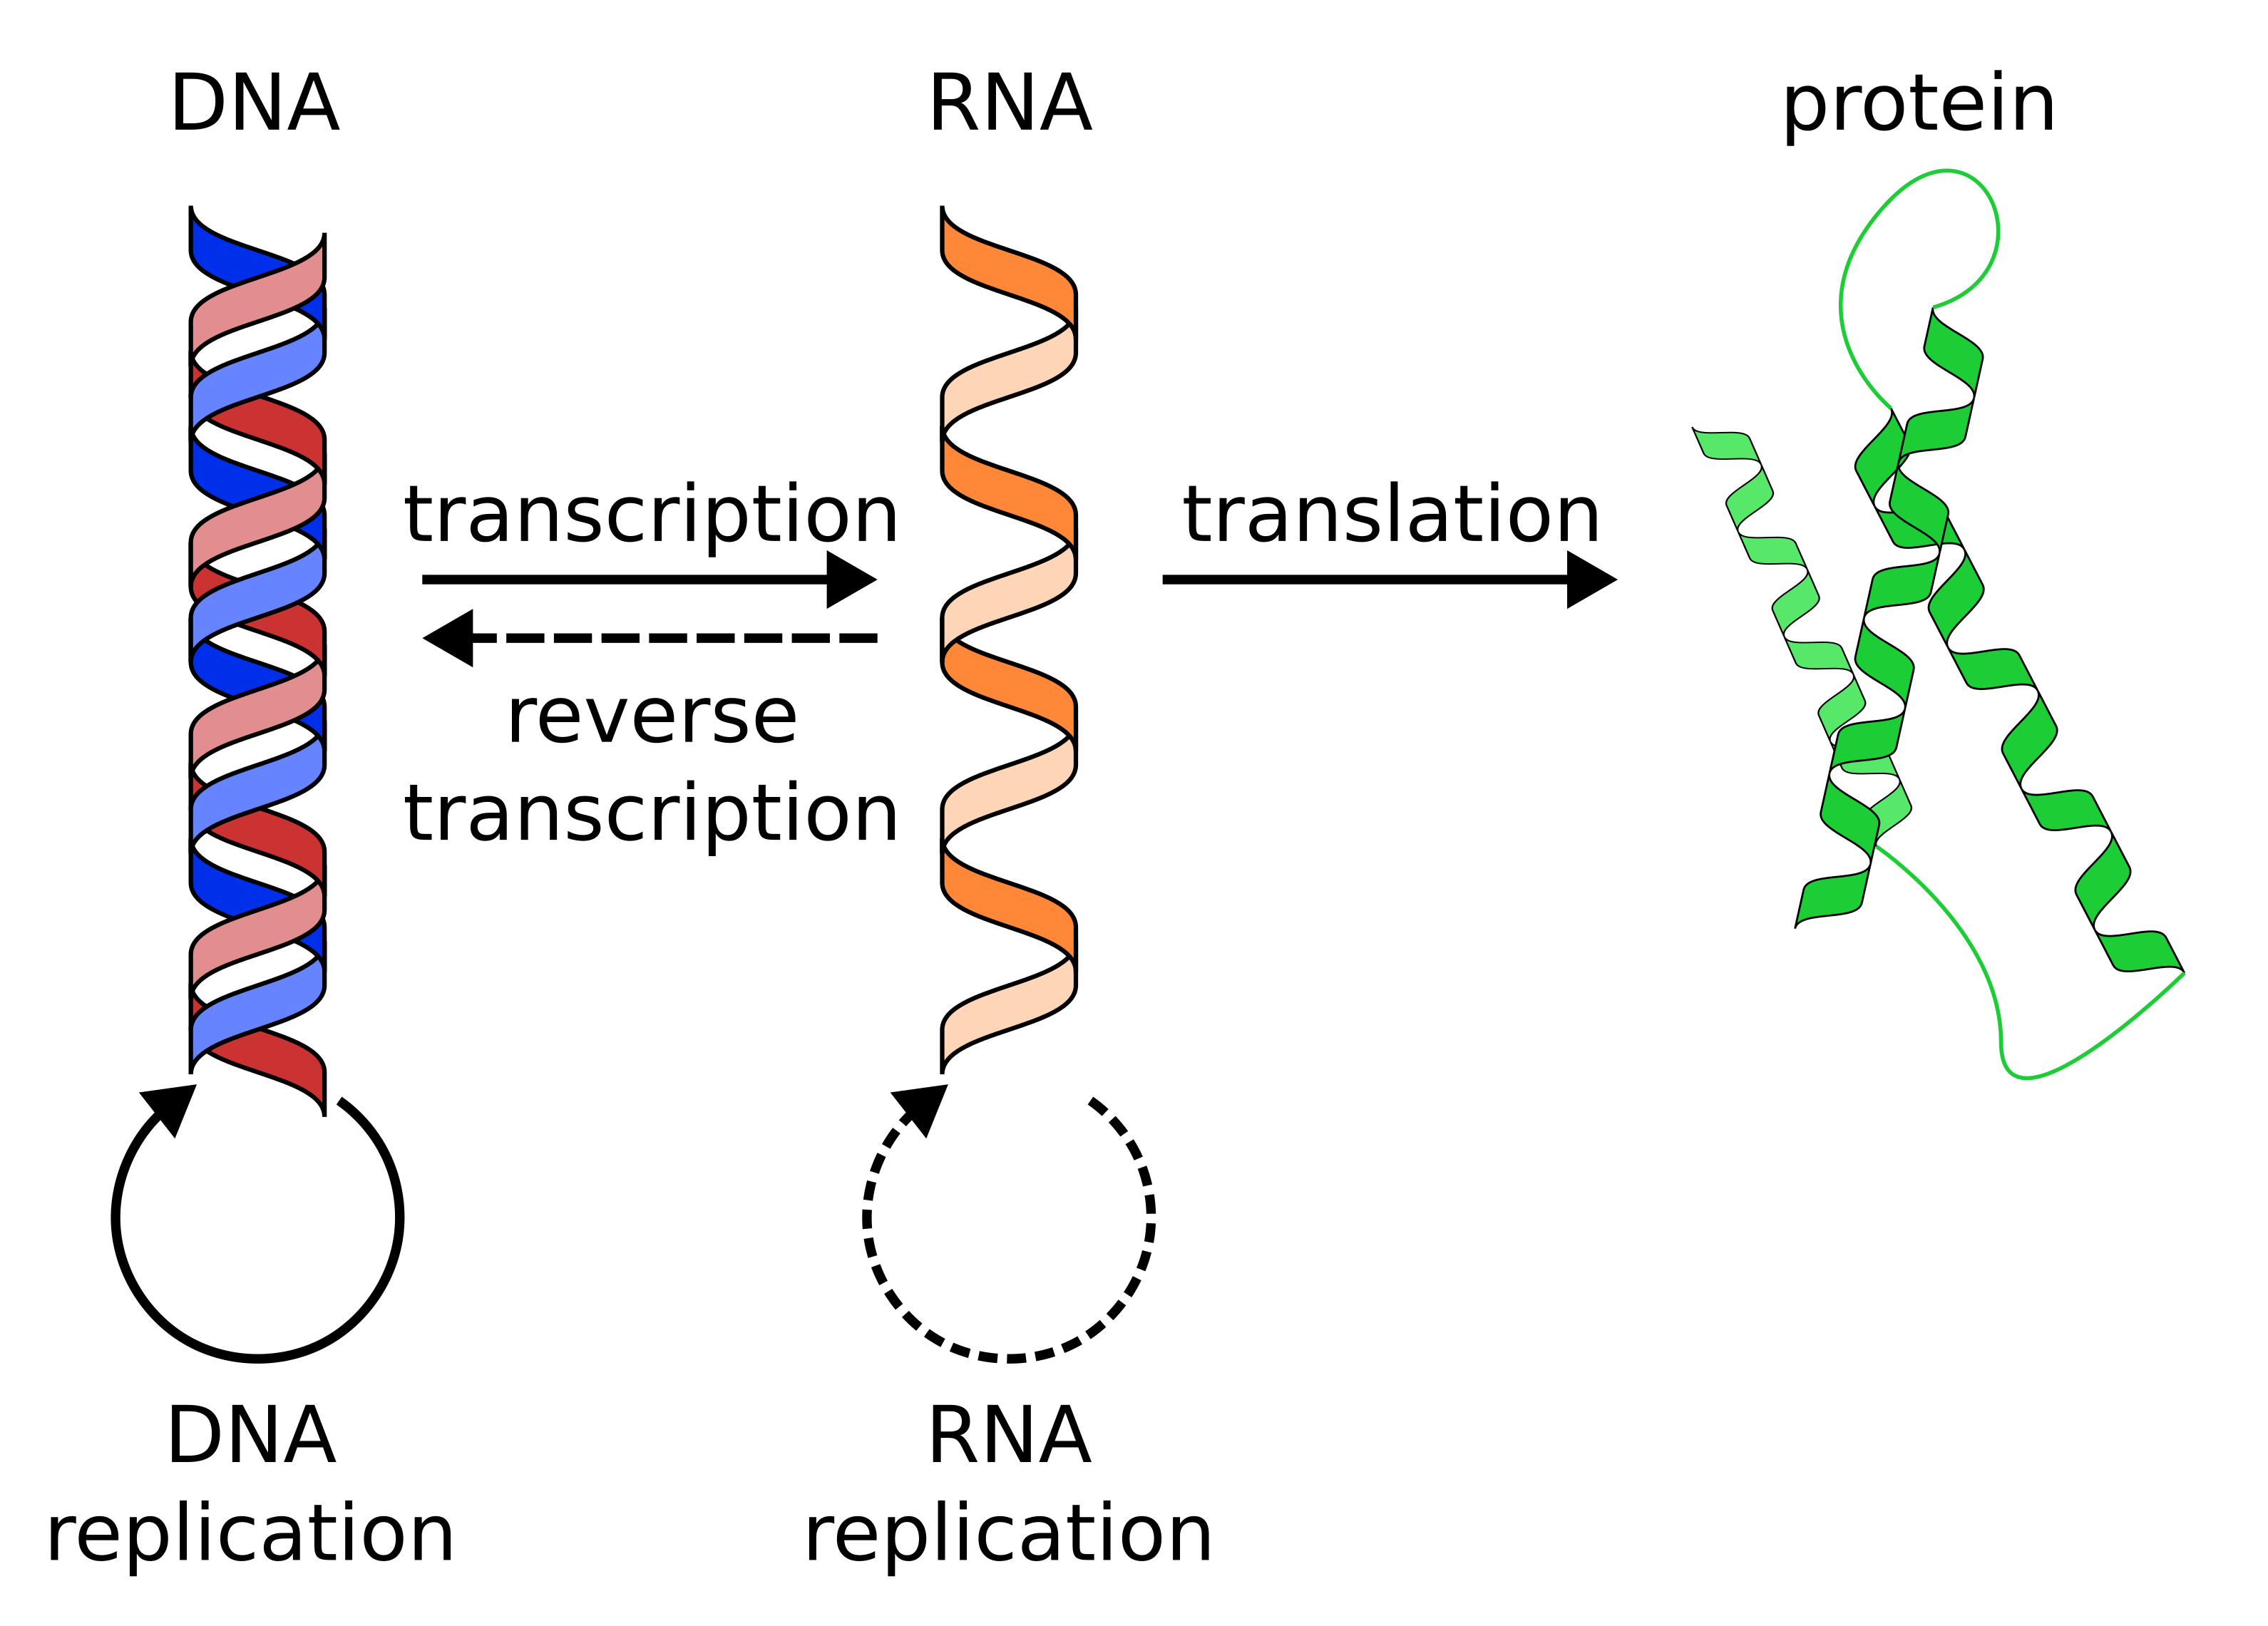
\includegraphics[width=0.7\linewidth]{ch.introduction/imgs/central_dogma.png}
    \caption{\textbf{The central dogma of molecular biology.} DNA transcribes to RNA, and RNA translates to protein. Solid arrows indicate the general flow of information in the system, and dotted arrows are special cases.}
    \label{fig:central_dogma}
\end{figure}

The central dogma of molecular biology describes the flow of genetic information within a biological system. Whereas in a computer information is stored in bits, which can be either zero (0) or one (1), genetic information is stored in nucleotides, which can be either adenine (A), cytosine (C), guanine (G), or thymine (T). DNA is composed of two large strands of these four nucleotides that together form a double helix. Both strands contain the same information, but where there is a nucleotide A on one strand, there is always a corresponding nucleotide T on its complementary strand, and similarly for C and G. RNA, on the other hand, is a similar molecule but is typically single-stranded. It is transcribed from DNA and shares a similar nucleotide composition but replaces thymine (T) with uracil (U). RNA serves as the bridge between DNA and proteins. Through the process of translation, the information encoded in RNA is decoded and used to assemble chains of amino acids, known as proteins. Proteins carry out various tasks in our bodies, such as enabling chemical reactions, transporting other molecules, providing structure, and acting as regulators of DNA transcription and RNA translation.

Far from all the human DNA is transcribed to RNA, and not even all RNA translates to protein. As a general rule of thumb, we distinguish DNA sequences that get transcribed into RNA as genes. The human genome contains approximately 20,000 protein-coding genes, and these genes cover only 1.5\% of the genome\cite{Piovesan2019}. Early molecular biologists mainly focused on protein-coding genes, thus the remaining 98.5\% of the DNA got known as ``junk DNA'', a controversial term in the field\cite{Graur2013}. Recent research has revealed that around 10\% of human DNA is functional\cite{Graur2013}, although some estimates suggest that 
as much as 80\% of DNA plays a role in at least one biochemical process\cite{encode2012}.

\section{Gene expression regulation}

Even though all cells of an organism contain identical DNA, they use completely different sets of genes. This is possible due to the tight regulation of gene expression, for which cells have a wide array of tools at their disposal. This thesis mainly focuses on transcription factors in gene regulation and chromatin context.

\subsection{Transcription Factors}

A typical gene consists of its coding regions (exons), noncoding regions (introns), and the start site (promoter). The promoter functions as a location where general transcription factors (GTFs) bind, which in turn recruit RNA polymerase II (RNAPII). RNAPII is the protein complex responsible for transcription and is responsible for reading out the DNA of a gene and converting it to RNA. Even though the presence of general transcription factors and a promoter is generally enough for transcription to occur\cite{Haberle2018}, its regulation occurs through the interplay of transcription factors and enhancers (figure \ref{fig:TF}). Enhancers are small regions on the DNA, typically a few hundred base pairs in length. TFs bind in these enhancers, based on specific DNA sequences (motifs). Different TFs have different functions, and some help with the recruitment of RNAPII and GTFs, whilst others help with making the promoter or other DNA sequences more accessible. Transcription factors thus act like switches, determining whether transcription should be turned up or down in response to various signals and conditions.

\begin{figure}[h]
    \center
    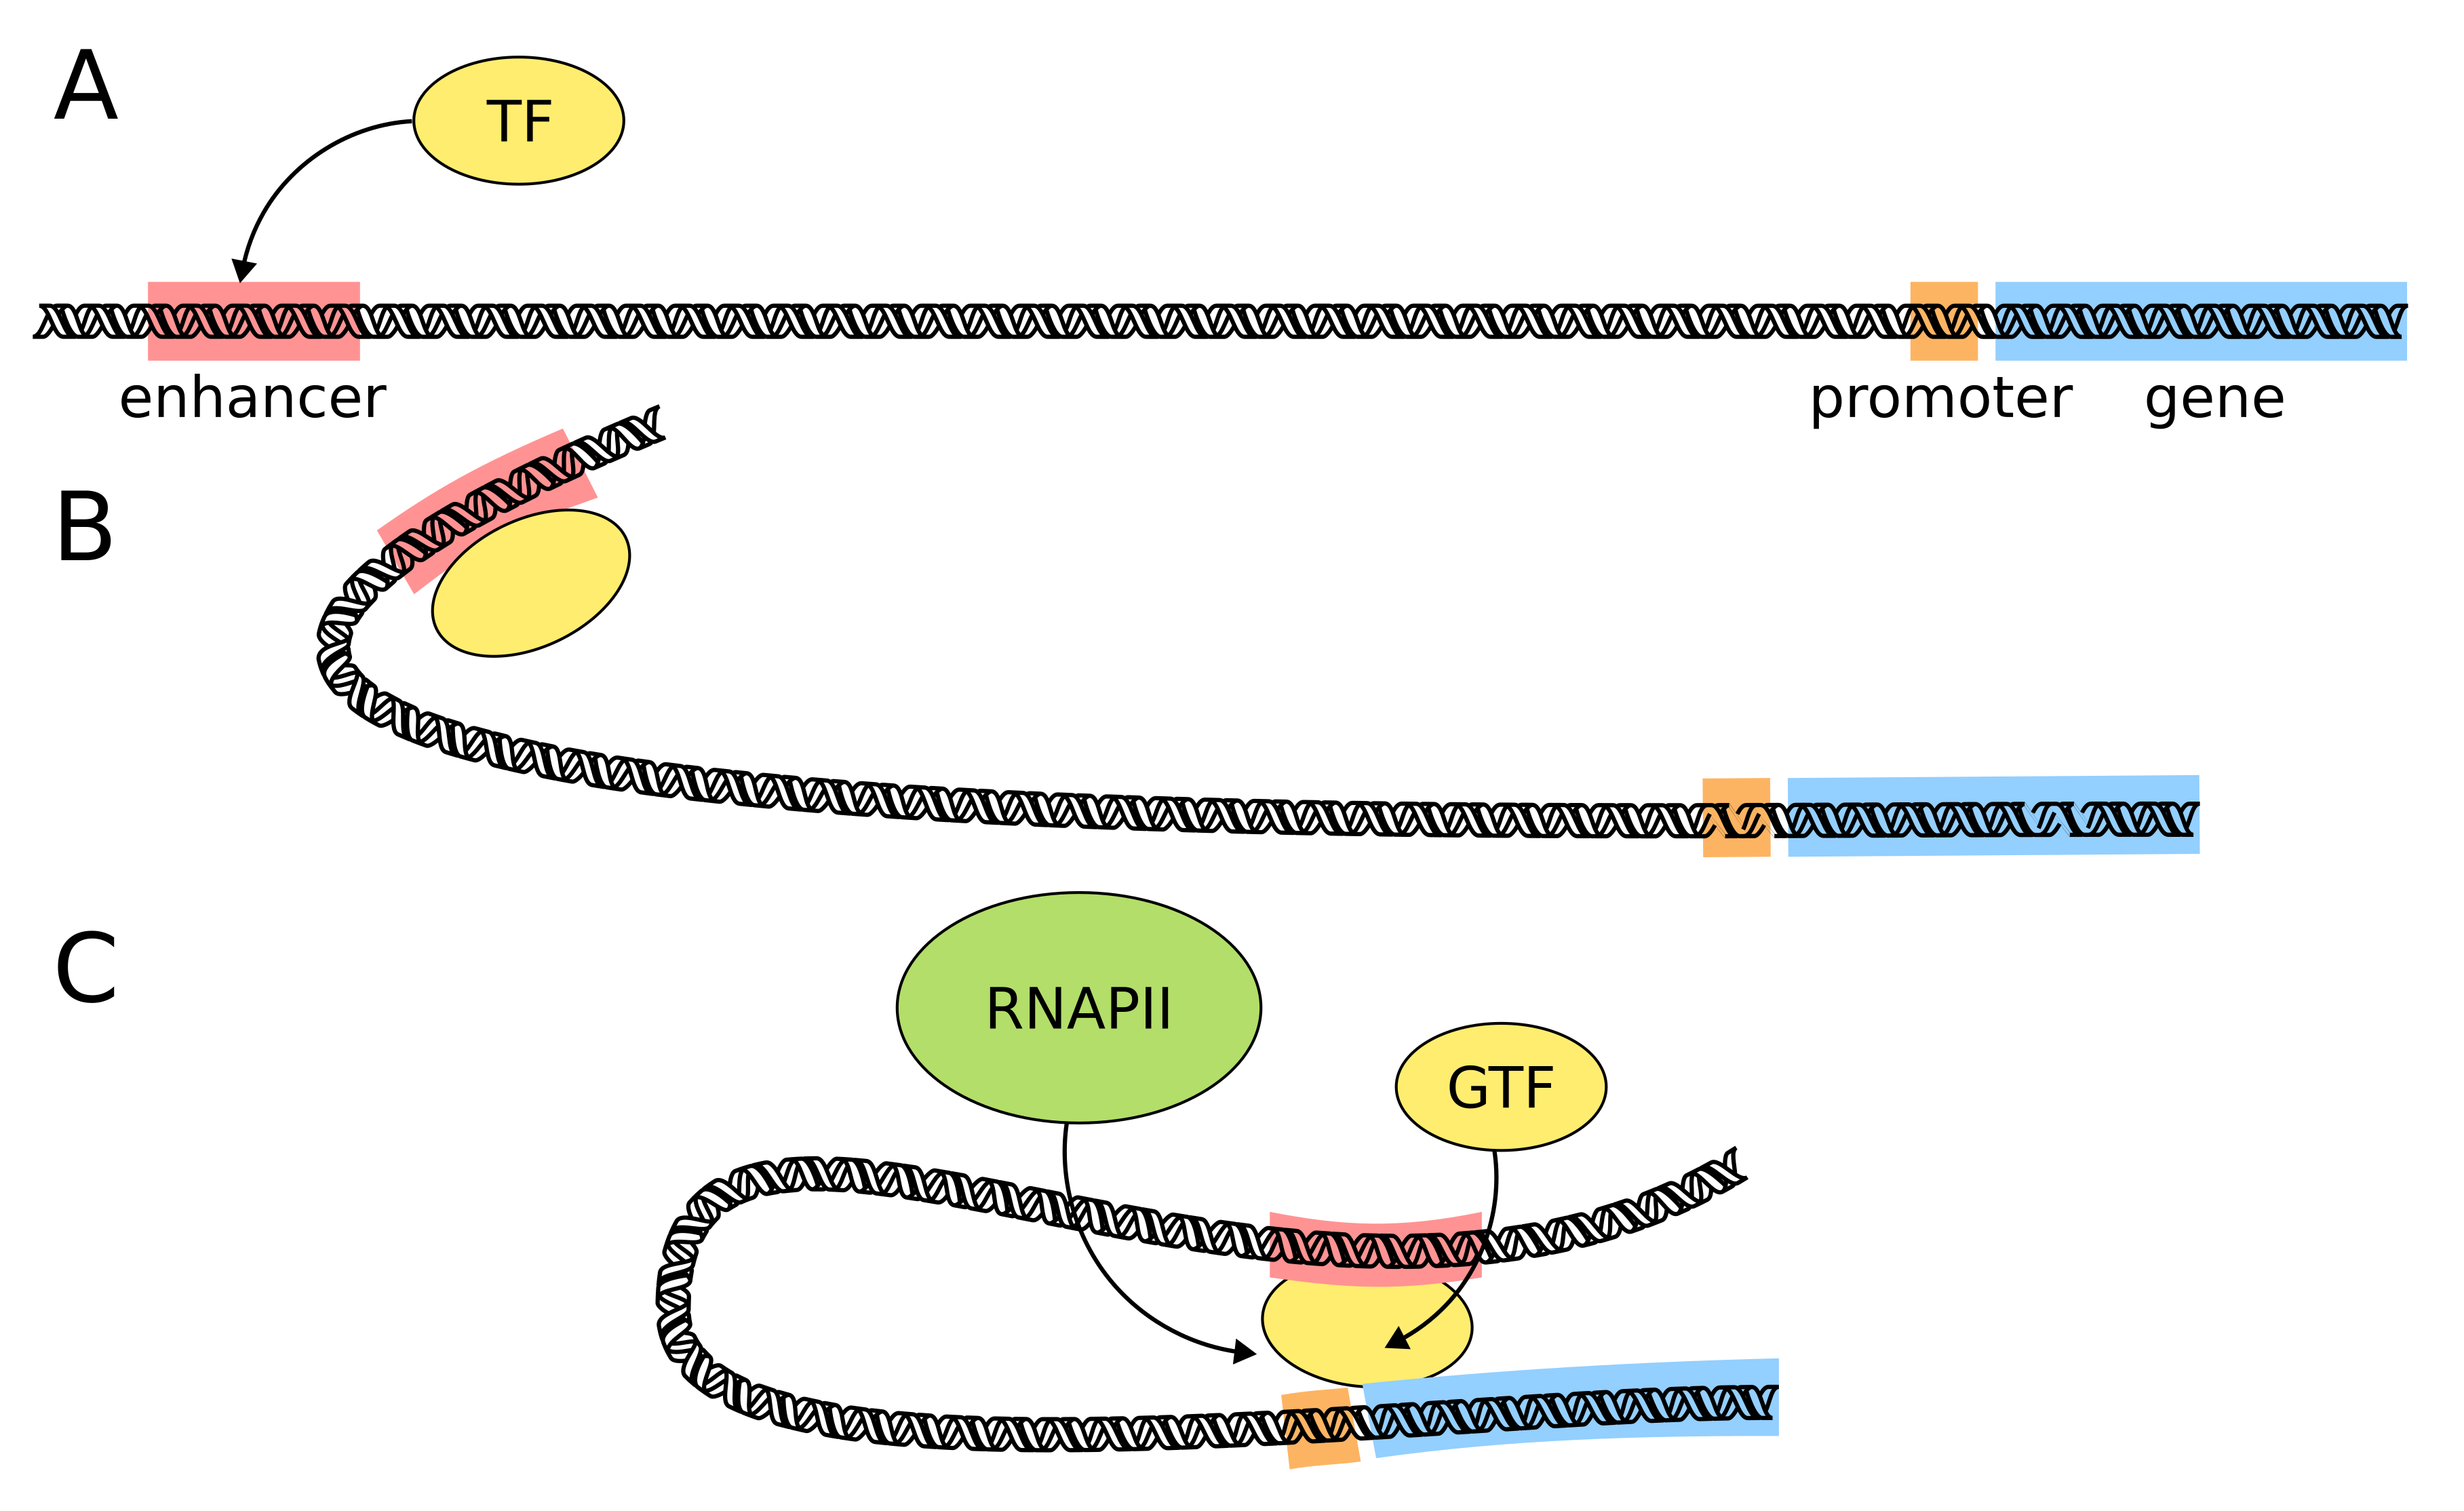
\includegraphics[width=0.8\linewidth]{ch.introduction/imgs/transcription_factor.png}
    \caption{\textbf{Gene regulation by transcription factors.} \textbf{(A)} A gene (blue area) with a promoter upstream (orange) and a "distal" enhancer (red). A transcription factor (TF) binds to the enhancer. \textbf{(B)} The TF causes the DNA to "loop", bringing the enhancer and TF closer to the promoter. \textbf{(C)} Because of the DNA loop, the distal enhancer and promoter are in close proximity, and the TF can increase transcription by recruiting general transcription factors (GTFs) or RNA polymerase II (RNAPII). Usually, multiple enhancers and multiple transcription factors per enhancer are involved, and their combined action regulates gene expression.}
    \label{fig:TF}
\end{figure}

Gene expression is regulated through the combined action of many (cis-)regulatory elements, such as the promoter and enhancers, but also silencers and insulators\cite{Spitz2012}. Silencers have a similar but opposite function to enhancers, they downregulate transcription. Insulators regulate the distances between enhancers/silencers and the promoter. Insulators function by recruiting proteins that create a physical 
barrier, effectively blocking interactions between regulatory elements located on opposite sides of the insulator. An insulator in between an enhancer and promoter can, for instance, block the TFs bound on the enhancer from recruiting GTFs to the promoter.

There are usually multiple transcription factors binding at a single enhancer, and the function of an enhancer should be considered at the combinatorial level. The positioning of motifs in an enhancer is known as the motif grammar, and includes, for instance, the presence (or absence) of certain motifs, the order of these motifs, their orientation, and spacing. Studying motif grammar is a hard problem, as there are many permutations of motifs possible in a single enhancer. Moreover, motif grammar changes based on the cell type, and it is costly to experimentally validate predictions.

\subsection{Chromatin context}

To be able to fit two meters of DNA into each cell, DNA needs to be carefully folded. Chromatin is the term for the structure of DNA, which consists of DNA and proteins. The main proteins in chromatin are histones. Histones are protein complexes around which DNA tightly wraps, forming a structure called a nucleosome. Nucleosomes are the basic units of chromatin (fig. \ref{fig:histones}). Next to the structural role of chromatin,  it also plays an important part in gene expression regulation, and can both promote and inhibit gene expression.

\begin{figure}
    \center
    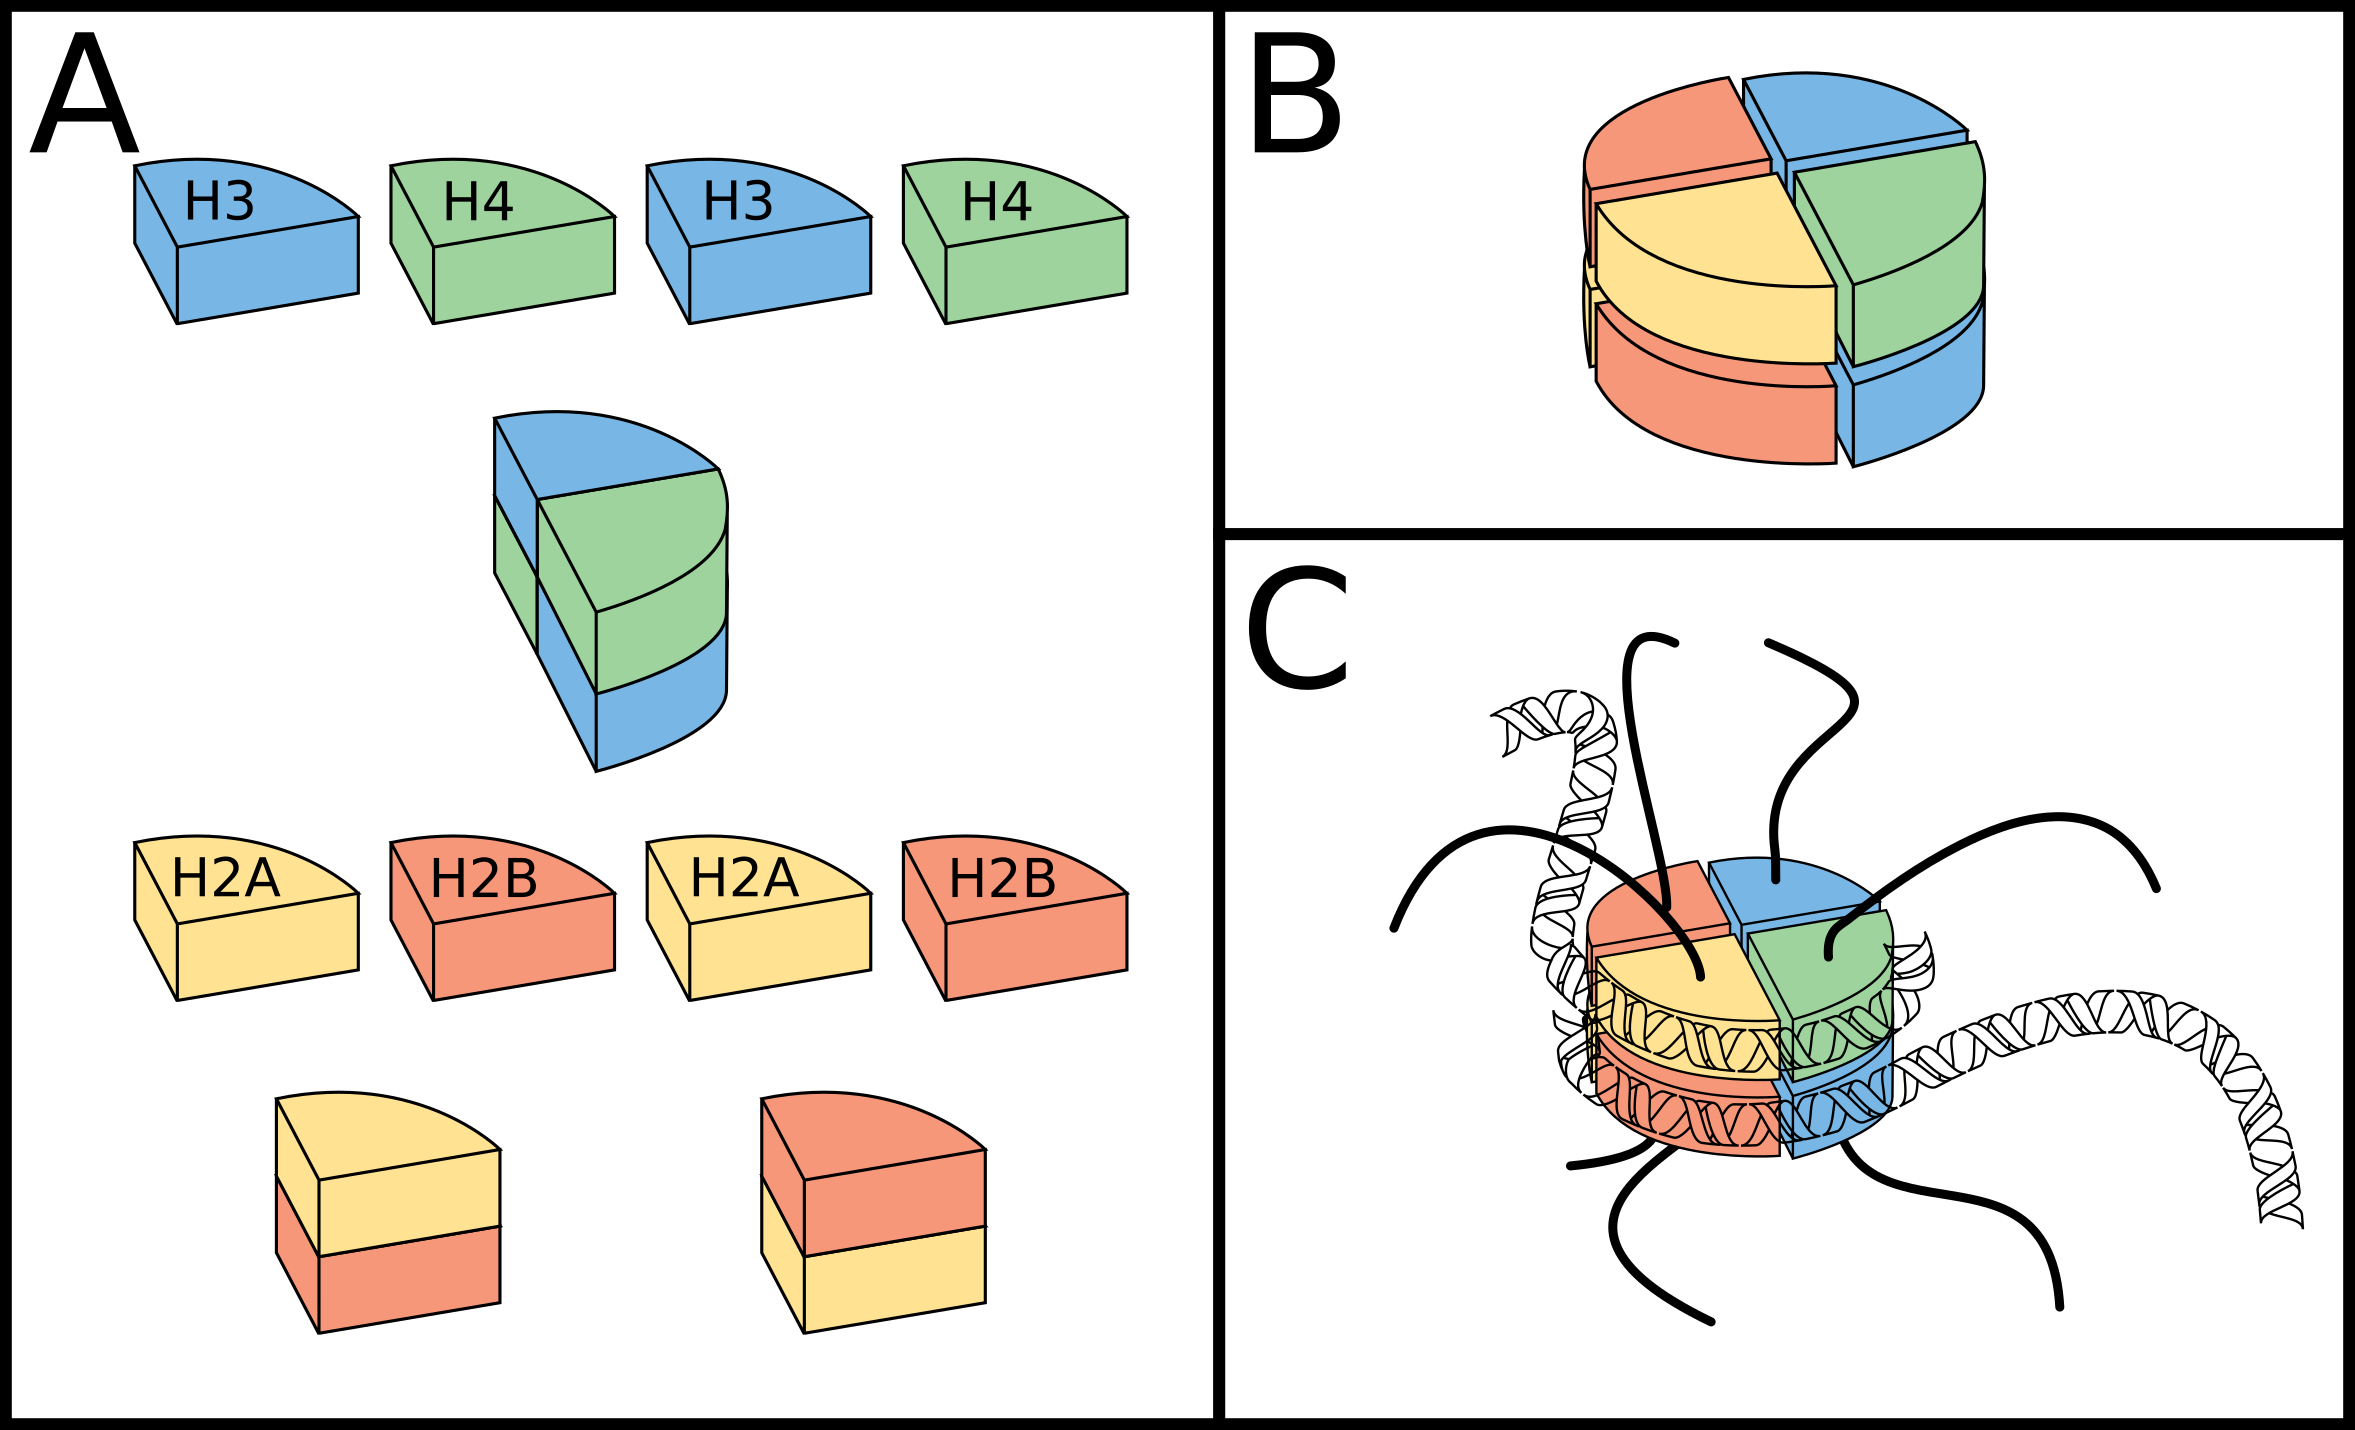
\includegraphics[width=0.8\linewidth]{ch.introduction/imgs/histones.png}
    \caption{\textbf{The nucleosome consists of a histone complex with DNA wrapped around it.} \textbf{(A)} The eight subunits of a histone complex. \textbf{(B)} An assembled histone complex. \textbf{(C)} A histone with DNA wrapped around it. DNA wraps twice around a histone in 146 base pairs. Chemically modifiable tails stick out of the histones, which are important markers and regulators of chromatin state.}
    \label{fig:histones}
\end{figure}

Histones have long protruding tails, that serve as a binding scaffold for protein complexes. These complexes in turn remodel the chromatin, for instance, to condense it, which blocks access of TFs to the DNA. The tails are chemically modifiable, such as by acetylation-, methylation-, and phosphorylation. The way to describe the modifications is by adding the histone number, amino acid, and type of modification. A well-studied modification is H3K27ac, which is the acetylation (ac) of the 27th amino acid, which is Lysine (K), of histone 3 (H3). H3K27ac tends to be associated with an open chromatin structure, allowing easier access to the DNA, and thus promoting the expression of nearby genes\cite{Creyghton2010}. Another example is the H3K9me3 modification, which is the tri-methylation (me3) of the 9th amino acid, Lysine (K), of histone 3 (H3). H3K9me3 is associated with a high nucleosome density and is generally a mark for repressed DNA\cite{Barski2007}.

Nucleosomes are not evenly spread out along the DNA. There are stretches with barely any nucleosomes, called nucleosome-free regions or open chromatin, or regions with a high density of nucleosomes, called closed chromatin or heterochromatin. The general idea is that closed chromatin is so tightly folded that it is difficult for proteins such as TFs to read and bind to the DNA. The other extreme is open chromatin, where (almost) no nucleosomes are present. Here there is nothing to block proteins from accessing the DNA, and open chromatin is generally associated with active DNA\cite{Klemm2019}. In between open and closed chromatin is permissive chromatin, where nucleosomes are present, but the DNA is not folded so tightly that it has become inaccessible. 

Another way chromatin context regulates gene expression is by the specific positioning of nucleosomes. A sequence of 146 base pairs wraps twice around a histone complex. By wrapping around a histone, two motifs at +/- 73 bp distance can suddenly become adjacent. It is thus not surprising that nucleosome positioning is far from random, and plays an important role in gene expression regulation\cite{Jiang2009}.

Finally, another important aspect of gene regulation is DNA methylation, where methyl groups are added to certain regions of DNA. DNA methylation can cause genes to be "silenced" or turned off, as it prevents the cellular machinery from binding to the DNA and initiating gene transcription.

\begin{figure}
    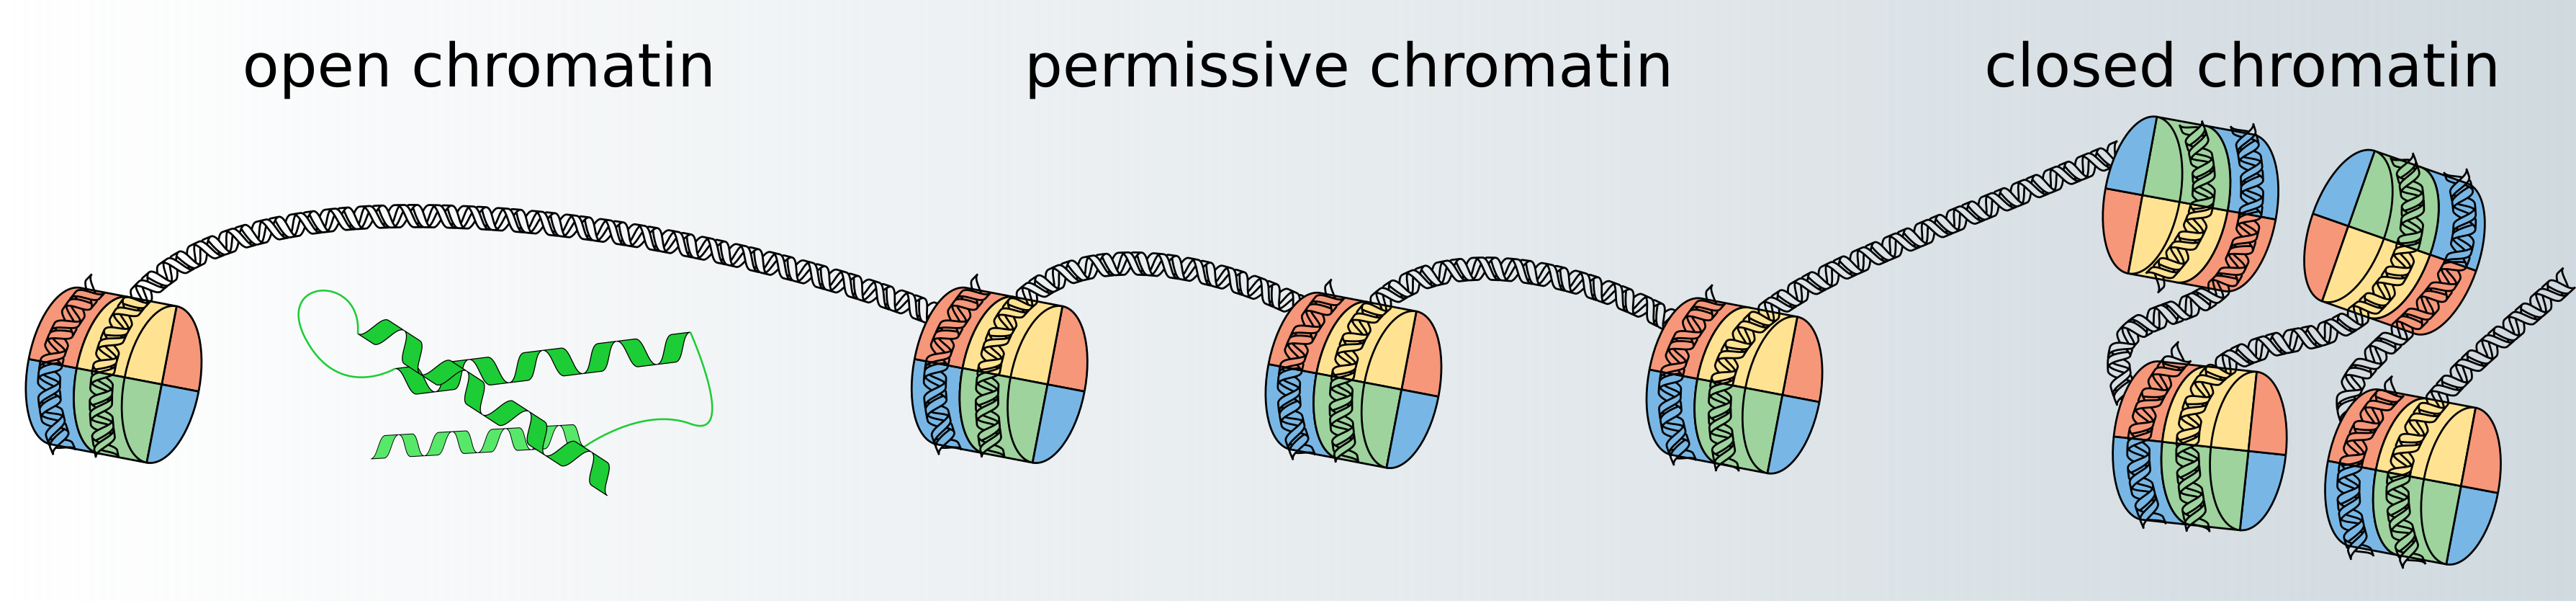
\includegraphics[width=\linewidth]{ch.introduction/imgs/accessibility_horizontal.png}
    \caption{\textbf{Schematic representation of how chromatin context regulates DNA accessibility}. When no histones are bound (open chromatin) transcription factors can easily scan the DNA for motifs and bind. Closed chromatin on the other hand is so tightly bound by histones that the DNA has become inaccessible for transcription factors. In between lies permissive chromatin, which, depending on the histone modifications is accessible for transcription factors.}
    \label{fig:accessibility}
\end{figure}

\subsection{Other gene regulatory modes}

There are many other ways gene expression is regulated, such as by regulating RNA degradation, post-translational modifications, and signal transduction. After transcription, RNA exists in the cell and gets translated into protein by ribosomes. Mammalian RNA has a lifetime of several minutes to days\cite{Yu2001}. But to be able to react to environmental changes, a cell is able to mark RNAs for degradation, for instance by poly-A tail removal. 

In addition, the activity and localization of proteins can be regulated by post-translational modifications. These modifications play an important role in fine-tuning the functionality of proteins and their interactions with other molecules. Many different post-translational modifications exist, such as phosphorylation, acetylation, sumoylation, and methylation. These modifications usually influence the protein's stability, shape, activity, and localization. Phosphorylation, for instance, can serve as a switch to activate or deactivate specific protein functions, ubiquitination marks proteins for degradation, and sumoylation is involved in proteins' stability and localization\cite{Mazur2012}.

Finally, chemical and physical signals also play an important role in regulating gene expression. Our bodies react to light by keeping a day-night schedule, produce melanin after exposure to UV light, and grow our muscles after training. A particularly interesting example of how such signals regulate gene expression is the electrical signal that flatworms use during regeneration. A flatworm is a highly regenerative animal, you can cut off its head and tail, and the worm will regrow back its head and tail. It turns out that flatworms make use of an electrical gradient along their body that helps cells decide where in the body axis they are. When one cuts off the head and tail of a flatworm, whilst simultaneously interfering with this electrical gradient, you get flatworms that grow back two heads or tails\cite{Levin2014}.

\subsection{Gene regulatory networks}

Mapping how protein products of genes (e.g. transcription factors) influence the protein level of other genes is crucial for understanding how cellular processes are regulated. A common abstraction to understand gene-gene interactions is a gene regulatory network.

The first concept of gene regulatory networks was proposed by Roy Britten and Eric Davidson in 1969\cite{Britten_1969}. They observed that a cell (i) responds to an external signal; (ii) then produces its own signal as a response; (iii) transmits its own signal to receptors that do not perceive the external signal; (iv) then responds to its own signal, and finally (v) produces a protein as a response. Without modern knowledge of gene regulation, they then predicted what the minimum requirements are for such a system. One of the things they correctly predicted was the existence of transcription factors and promoter sequences. It took Eric Davidson more than 30 years to experimentally validate his original predictions\cite{Davidson_2002}.

Gene regulatory networks come in many forms and shapes but are often modeled and visualized with direct gene-gene interactions (fig. \ref{fig:network}A). This means for instance that the protein product of gene $\alpha$ directly regulates the protein product of gene $\beta$, ignoring all steps, such as transcription and DNA binding, in between. Even though this is a gross oversimplification of gene-gene interactions, these simple models can already exhibit complex behavior. One of the older and more well-known examples of complex behavior from a simple model is a Turing pattern, first described by the famous computer scientist Alan Turing\cite{Turing1952}. One specific Turing model, the Gierer-Meinhardt model, consists of two genes, gene $\alpha$, and gene $\beta$, where gene $\alpha$ upregulates itself and gene $\beta$, but gene $\beta$ inhibits gene $\alpha$ (fig. \ref{fig:network}B). When modeling this simple two-gene network in a spatial setting it produces complex patterns (fig. \ref{fig:network}C), of which similar patterns have been observed in nature, such as the skin pattern of a pufferfish (fig. \ref{fig:network}D).

\begin{figure}[H]
    \center
    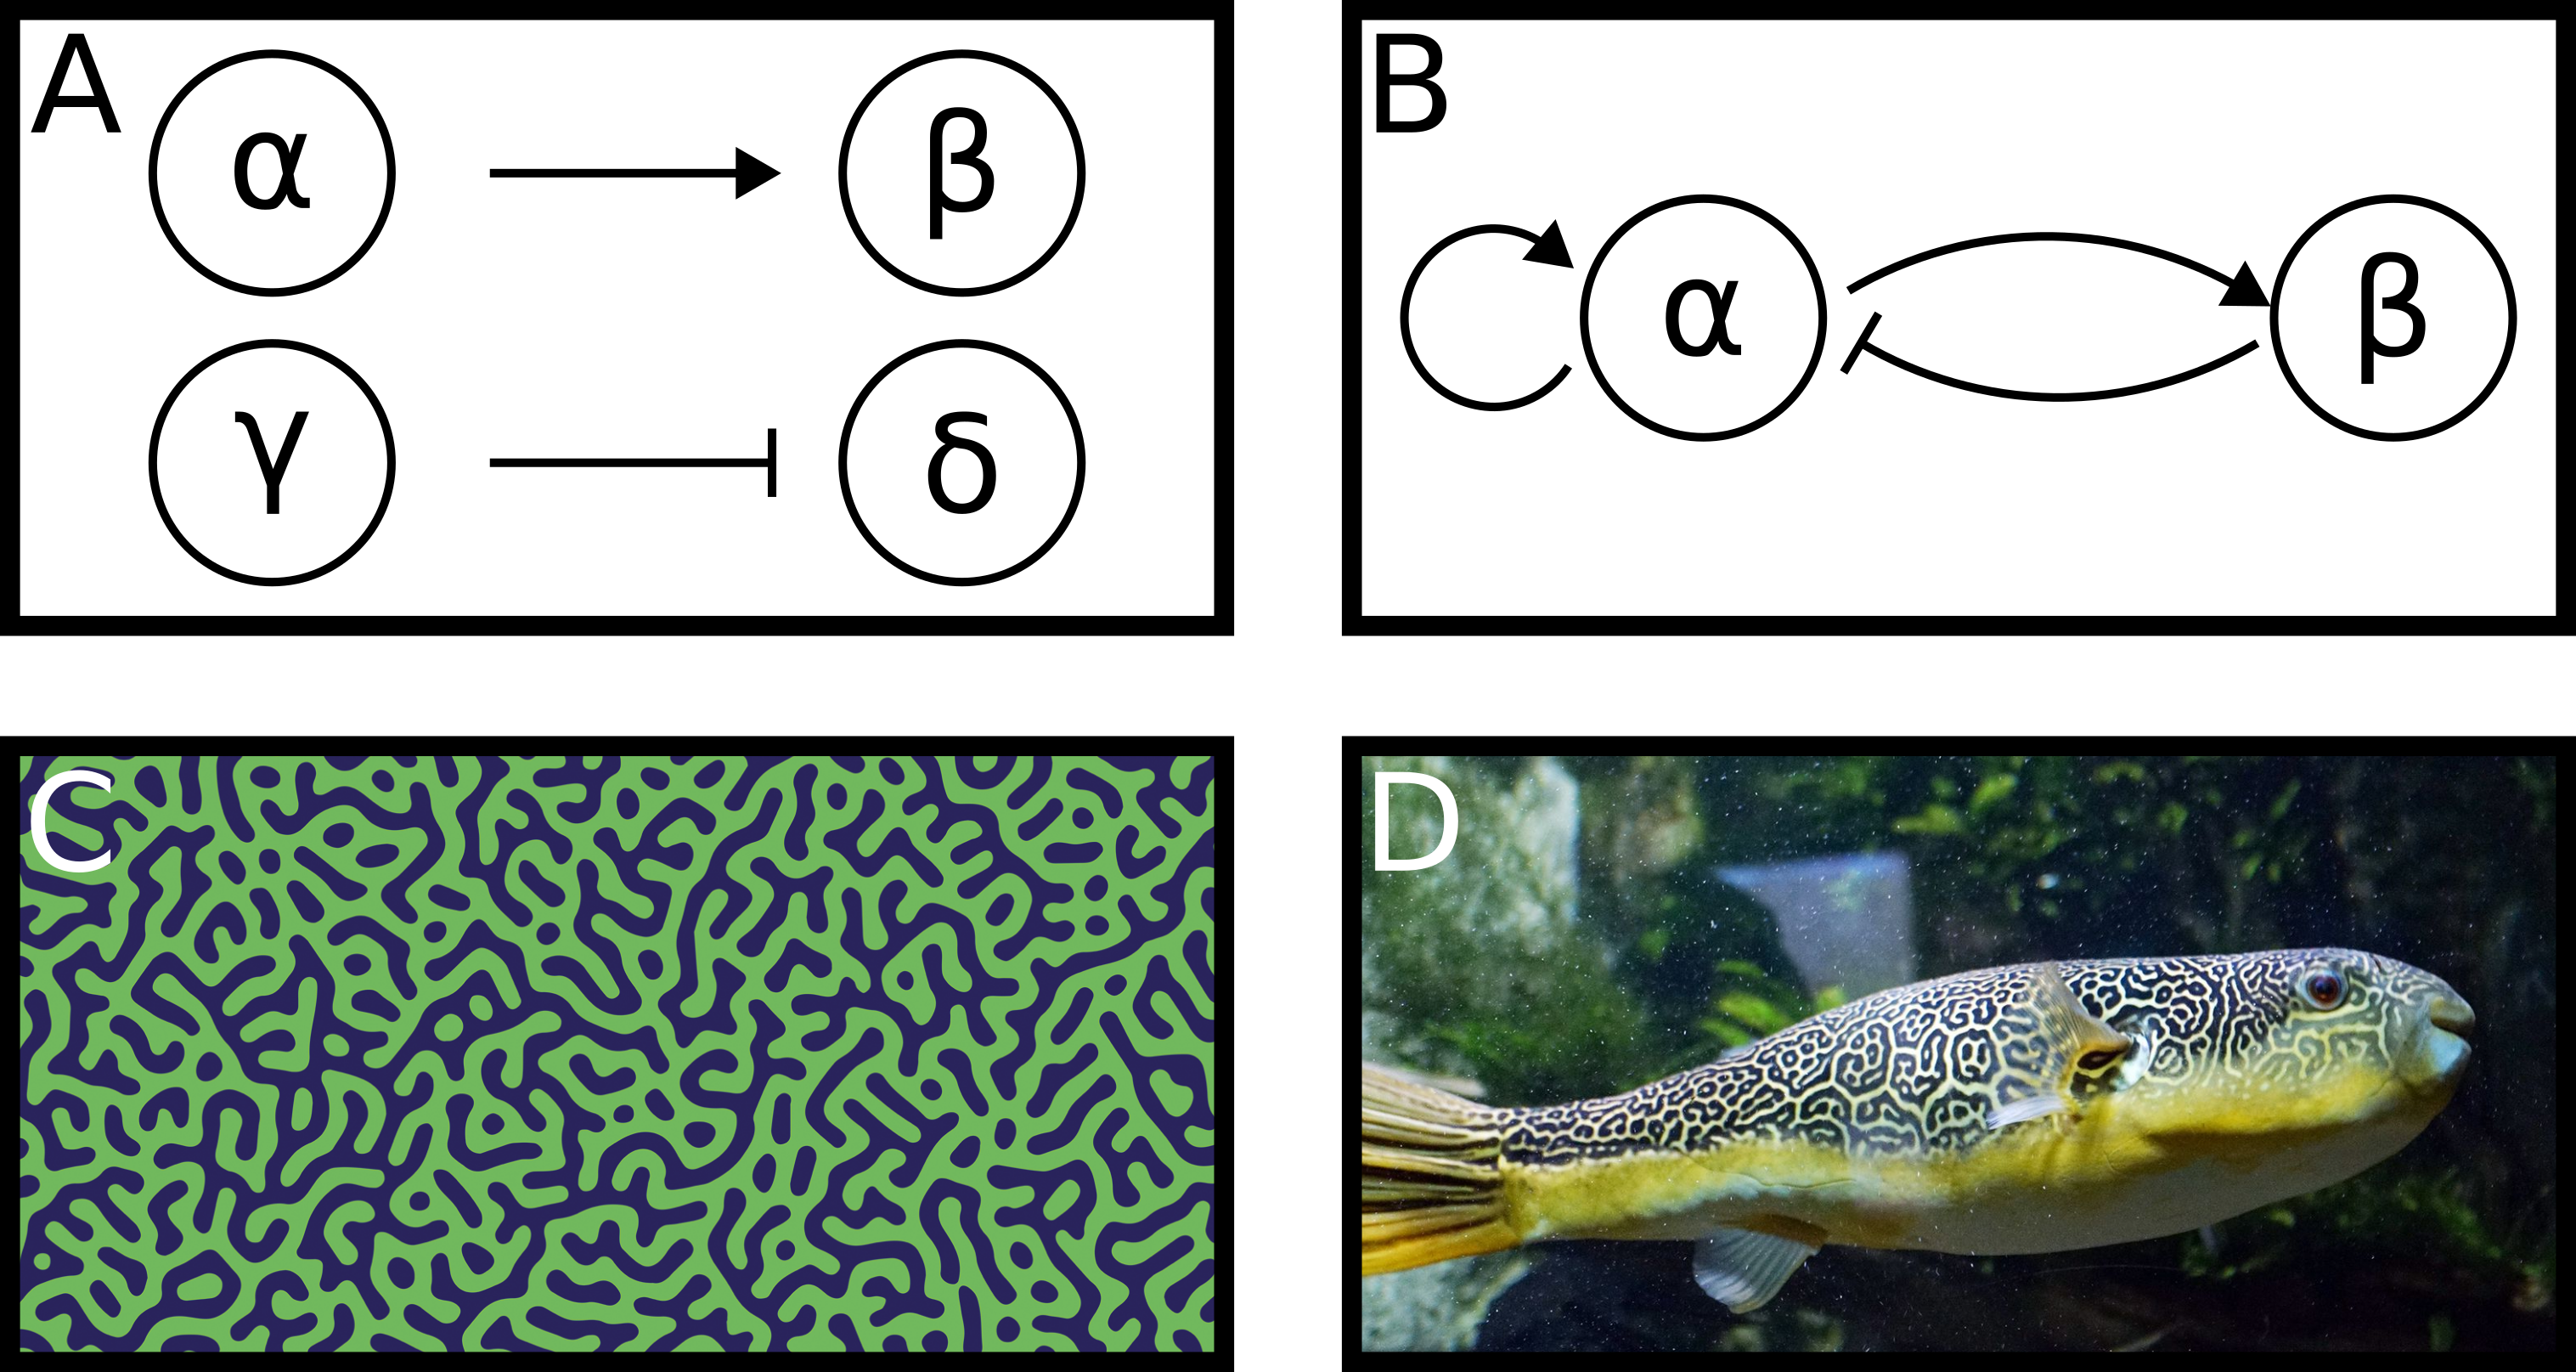
\includegraphics[width=0.8\linewidth]{ch.introduction/imgs/network.png}
    \caption{\textbf{Basic gene regulatory networks.} (\textbf{A}) the standard schematic way of representing gene-gene interactions. Gene $\alpha$ upregulates gene $\beta$, and gene $\gamma$ downregulates gene $\delta$. (\textbf{B}) Gierer-Meinhardt gene regulatory network, where gene $\alpha$ upregulates itself and gene $\beta$, and gene $\beta$ downregulates gene $\alpha$. (\textbf{C}) Simulation of the Gierer-Meinhardt gene regulatory network in a spatial context. (\textbf{D}) A Mbuna pufferfish with Turing pattern. Turing pattern from: https://www.nature.com/articles/s43588-022-00306-0 and pufferfish photo taken by Tiia Monto: https://en.wikipedia.org/wiki/Mbu\_pufferfish\#/media/File:Tetraodon\_mbu\_2.jpg}
    \label{fig:network}
\end{figure}

Mapping the relations between genes is a hard problem and unfeasible to do by hand. Not only can potentially any gene have an (in)direct effect on any other gene, but the potential interactions also depend on the cell type. The 20.000 human protein-coding genes have 20.000$^2$=400.000.000 potential direct interactions, and if we consider indirect interactions, cell type-specific interactions, and combinatorial interactions the number of potential gene networks explodes. To infer gene interactions at scale and make sense of the resulting networks we \textit{have} to make use of computational tools. The most common approach so far has been to measure RNA expression in a combination of settings and correlate the RNA expression of genes over these settings \cite{Zhang_2005,Margolin_2006}. Correlations above a certain threshold would indicate an (in)direct gene regulation. Adding more information to these networks, such as the chromatin state around genes\cite{Xu_2020,Kamal_2021}, improves the resulting networks. However, practically all gene regulatory network inference approaches compare cell states (e.g. liver vs. skin), so the inferred gene networks are specific for these comparisons. In chapter 2 we discuss the latest developments in gene regulatory network inference.

\section{Genomics analysis}

In order to study the regulation of gene expression one needs to experimentally measure the molecular changes between conditions. Genomic experiments can usually be broken down into two main stages: wet lab work,  and computational analysis. The wet lab phase involves hands-on experimentation with physical materials like chemicals and biological samples, DNA isolation, and DNA sequencing. In contrast, the computational analysis is concerned with the interpretation and analysis of the data generated by the wet lab.  In this thesis, three different types of sequencing assays have been used and analyzed (ATAC-seq, ChIP-seq, and RNA-seq), and here I will briefly explain their wet lab and computational aspects. 

\subsection{Wet lab}

The Assay for Transposase-Accessible Chromatin using sequencing (ATAC-seq) is a technique employed to assess genome-wide chromatin accessibility\cite{Buenrostro_2015}. Chromatin accessibility is closely linked to DNA activity; accessible DNA regions tend to be associated with active gene expression, while less accessible regions often correspond to inactive DNA. ATAC-seq operates by introducing a protein known as Tn5 transposase into a biological sample. This transposase enzyme semi-randomly cleaves the genomic DNA. However, in cases where DNA is inaccessible, for instance, due to obstructive histone modifications, the Tn5 transposase is unable to reach and cleave the DNA. Consequently, smaller DNA fragments  represent accessible regions, as they could be cleaved. Subsequently, the smaller DNA fragments, typically less than 500 base pairs in length, are isolated and prepared for sequencing.

Chromatin ImmunoPrecipitation sequencing (ChIP-seq) is a technique used to pinpoint the locations of specific proteins in close proximity to DNA\cite{Robertson_2007}. These proteins are often transcription factors or histone modifications. The method typically starts with the fixation of chromatin with formaldehyde, effectively preserving its structure. Subsequently, the DNA is fragmented into small segments, typically around 200 base pairs in length. Next, the proteins of interest are bound by specific antibodies. These antibody-protein-DNA complexes are then isolated, for instance by using magnetic antibodies. In the final stage, the DNA, proteins, and antibodies are separated, leaving behind the DNA fragments of interest. These fragments are then prepared for sequencing.

RNA sequencing (RNA-seq) is a technique to assess the presence and abundance of gene transcripts within a biological sample\cite{Nagalakshmi2008}. The quantity of RNA transcripts serves as a proxy for both gene expression levels and the potential amount of corresponding protein products. The RNA-seq process begins by isolating all the RNA molecules from the sample. Subsequently, these RNA molecules are converted into complementary DNA (cDNA) through a process known as reverse transcription (Fig. \ref{fig:central_dogma}). The resulting cDNA then represents the abundance of gene transcripts within the sample. This cDNA then is ready for sequencing.

\subsubsection{Sequencing}

Sequencing is used to determine the precise order of nucleotides within a DNA sequence. In this introduction, our primary focus is on the sequencing by synthesis method \cite{Canard1994}, although several other techniques, such as chain-termination sequencing\cite{Canard1994}, Nanopore Sequencing\cite{Jain2016}, and Single-Molecule Real-Time Sequencing\cite{Levene2003}, are also available. Sequencing by synthesis takes place on a specialized surface referred to as a flow cell. The process begins with the addition of adapters to both ends of each DNA strand. Subsequently, the DNA is evenly distributed across the flow cell, with the adapters serving as anchors that firmly attach the DNA to the flow cell. Through polymerase chain reaction (PCR) amplification, the DNA strands, along with the adapters, are duplicated, resulting in the duplicated sequences anchored in proximity to their original. Repeating the process of PCR amplification leads to the formation of clusters of identical DNA sequences concentrated at various spots on the flow cell. Next, the flow cell undergoes a heating step, causing the DNA strands to become single-stranded. In a sequential manner, fluorescently labeled nucleotides are introduced into the flow cell. These nucleotides are each associated with a distinct color that is emitted upon their incorporation into the DNA strand. Throughout this process, a camera captures the emitted colors from each spot. The sequence of DNA is deduced by observing the order of colors emitted from each spot on the flow cell.

\subsection{Dry lab}

The outcome of sequencing is a data file, structured with as many lines as there were spots on the flow cell, with each line representing a DNA sequence (in FASTQ format). First, it is necessary to computationally remove the sequencing adapters from these sequences to prepare them for further analysis. The subsequent step involves aligning these sequences to a reference genome, a computationally intensive task given that FASTQ files typically contain several millions of reads, while genomes can be billions of nucleotides long. Following this alignment, a file is generated that maps each read to its corresponding position within the genome. In the context of RNA-seq experiments, the subsequent stages usually involve associating these genomic alignments with their genes. This process is relatively straightforward since the positions of genes are typically known. Researchers can simply count the number of reads aligned within each gene for each sample. However, in the case of ATAC-seq and ChIP-seq experiments, the regions of interest are usually not known in advance. Therefore, the initial task is to identify these regions. This is typically done through peak-calling algorithms\cite{Zhang2008,Stovner2019,Tarbell2019}. These algorithms search for regions (peaks) where the number of mapped reads exceeds a statistically defined threshold. The results from multiple samples in ATAC-seq, ChIP-seq, and RNA-seq experiments are generally aggregated into a table format, where each row corresponds to a gene or peak, and each column represents a different sample. The numerical values within each cell indicate the number of reads mapped to a particular gene/peak for a specific sample.

After obtaining a table with values for each sample, the subsequent steps depend on the research objectives. If one is interested in the difference between two relatively similar conditions, such as healthy vs. sick livers, a typical approach is to perform a differential expression analysis on the table\cite{deseq2}.  One can, for instance, apply a gene set enrichment analysis on the differentially expressed genes, a method to identify classes of genes that are over-represented in either condition. Other approaches include looking for specific mutations that only occur in one of the two groups. A more advanced approach would be to try to infer the liver gene regulatory network based on these samples. This network can then help by identifying dysfunctional genes and possible treatments. In RNA-seq experiments, the inference of gene regulatory networks is often achieved by examining correlations in gene expression over multiple samples. Gene-gene correlations that surpass a predefined threshold are considered indicative of causality. In ATAC-seq or ChIP-seq experiments, regulatory network inference frequently involves a transcription factor motif analysis on the identified peaks. Ideally, both RNA-seq and ATAC/ChIP-seq data are combined to construct more accurate gene networks.


\begin{figure}
    \center
    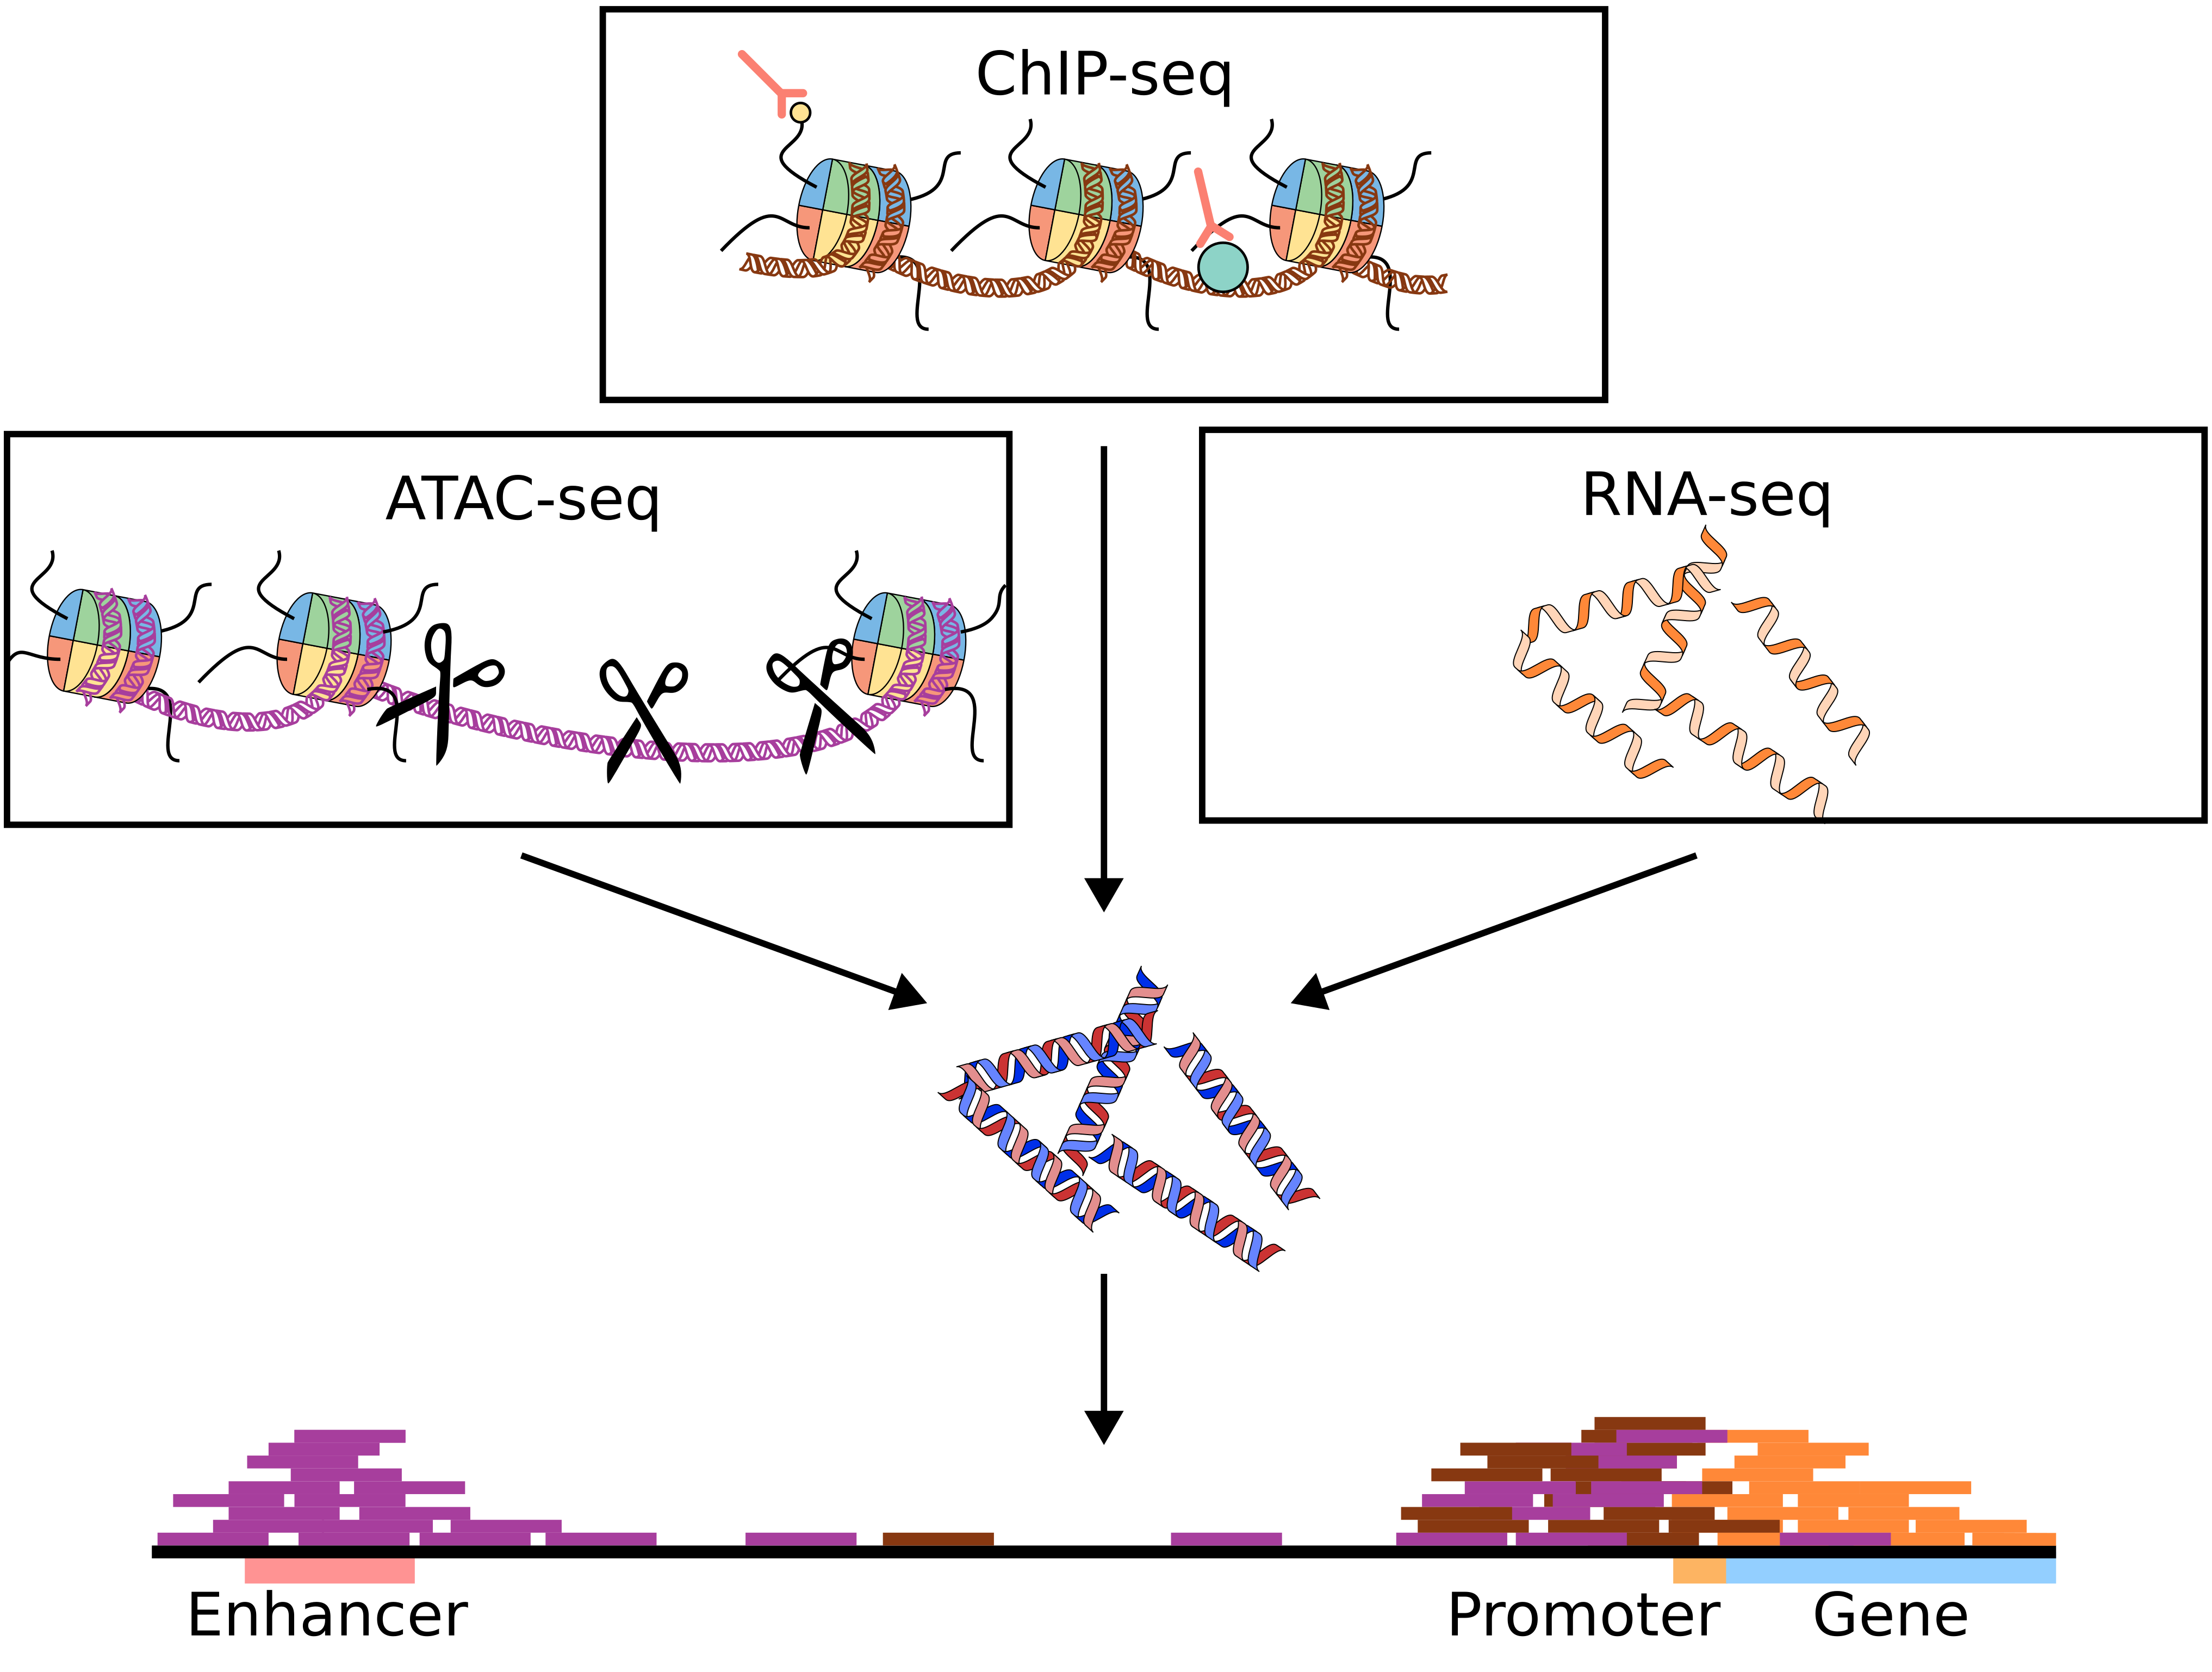
\includegraphics[width=0.8\linewidth]{ch.introduction/imgs/analysis.png}
    \caption{\textbf{Schematic overview of ATAC-seq, ChIP-seq, and RNA-seq and their computational analysis.} ATAC-seq is a technique that semi-randomly cleaves accessible DNA. Short DNA sequences thus represent accessible DNA. ChIP-seq is a way to isolate DNA sequences with specific proteins (usually TFs or histone modifications) in proximity. By filtering out the DNA after sonication with the bound antibodies (orange) you are left with DNA that was in close proximity to the protein of interest. RNA-seq is a technique for the estimation of the number of transcripts per gene. By reverse transcription the RNA gets converted into cDNA. The DNA these techniques produce can then be sequenced. After sequencing the DNA is computationally mapped to the genome by the dry lab, after which the real analysis starts. }
    \label{fig:analysis}
\end{figure}

In Chapter 3 and Chapter 4, I introduce dry lab tools seq2science and qnorm respectively. Seq2science is a preprocessing pipeline, that requires FASTQ files as input and runs standard analyses based on the files. Qnorm is a quantile normalization package, a common normalization technique to apply on count tables. Seq2science and qnorm streamline a significant portion of the dry lab workflow, resulting in standardized analyses and freeing up time for computational analysts for data exploration.

\subsection{Single-cell}

A significant drawback of traditional sequencing is that it aggregates the signal of all the cells present in a sample. If we were to take a biopsy of a liver, it would consist of a combination of liver cells (hepatocytes), blood cells, fat cells, etc., and sequencing this combination would result in a compound signal over cell types. This is why this type of sequencing has become known as bulk sequencing. Relatively recently, new techniques have been developed to separate all cells in a sample, give them cell specific sequencing adapters and thus perform RNA- or ATAC-seq on each cell separately\cite{Buenrostro2015_sc,Tang2009}. This type of data gives unprecedented detail in analyses and has been welcomed as a major improvement over bulk sequencing.

A major downside of single-cell sequencing, however, is that the data analysis is significantly harder. Whereas originally one would compare for instance a healthy liver vs. a sick liver, now there are thousands of liver cells separated over multiple cell types to compare. Moreover, the hardware that was used for the original bulk analyses is suddenly not powerful enough to deal with the enormous increase in data. Furthermore, statistical methods developed for bulk analyses are sometimes not appropriate anymore, as for instance, a cell has two copies of each chromosome, so genomic assumptions of continuous distributions of reads are broken. Similarly, single-cell RNA-seq count tables are sparse, which means they are filled with zeroes. This can be caused by biological reasons, simply the gene is not expressed, or by technical reasons, where not enough transcripts are sequenced in a cell \cite{Jiang2022}. Moreover, single-cell sequencing has the problem that it is extremely sensitive to batch effects, with major differences between who did the sequencing and when.

Regardless of these downsides, single-cell sequencing is a promising technique that has been quickly adopted in the field of genomics. It has given the field a new appreciation for the complexity of biology. In chapter 7 we TODO SCEPIA

\section{Evolutionary development (evo-devo)}

A single fertilized egg cell multiplies and develops into a complex collection of trillions of cells by the time we reach adulthood. How does each cell know where it is positioned in the body and what to develop into? The field of evolutionary development (evo-devo) studies development from an evolutionary point of view. In the 1980s scientists discovered a set of genes in fruit flies, which when mutated, were responsible for strange bodily transformations. A mutation in these genes caused flies to grow legs instead of antennae from their mouths\cite{Schneuwly1987} or flies to develop a second pair of wings\cite{Weatherbee1998}. This work was revolutionary at the time as it showed that (precursor) antennae cells contain all the information necessary to build legs. The group of genes responsible for these mutations are transcription factors known as HOX genes.

The embryonic development of a fruit fly starts as a worm-like larva consisting of multiple repeated segments. The gene expression of HOX genes determines the identity of each and guides its growth. For example, the \textit{lab} HOX gene is expressed at the frontal part of the larva, indicating surrounding cells this area will develop into the mouth of the fly\cite{Hughes2002}. Similarly, the \textit{Antp} HOX gene indicates leg formation and is expressed in the mid-section of the larva. Interestingly, HOX genes are found in nearly all animals, where they play an important role in the spatial organization of the organism. What makes Hox genes particularly fascinating is that their order on the chromosome is the same as the spatial ordering along embryos. This concept is called spatial colinearity, something we have no clear understanding of\cite{Gaunt2015}.

\begin{figure}
    \center
    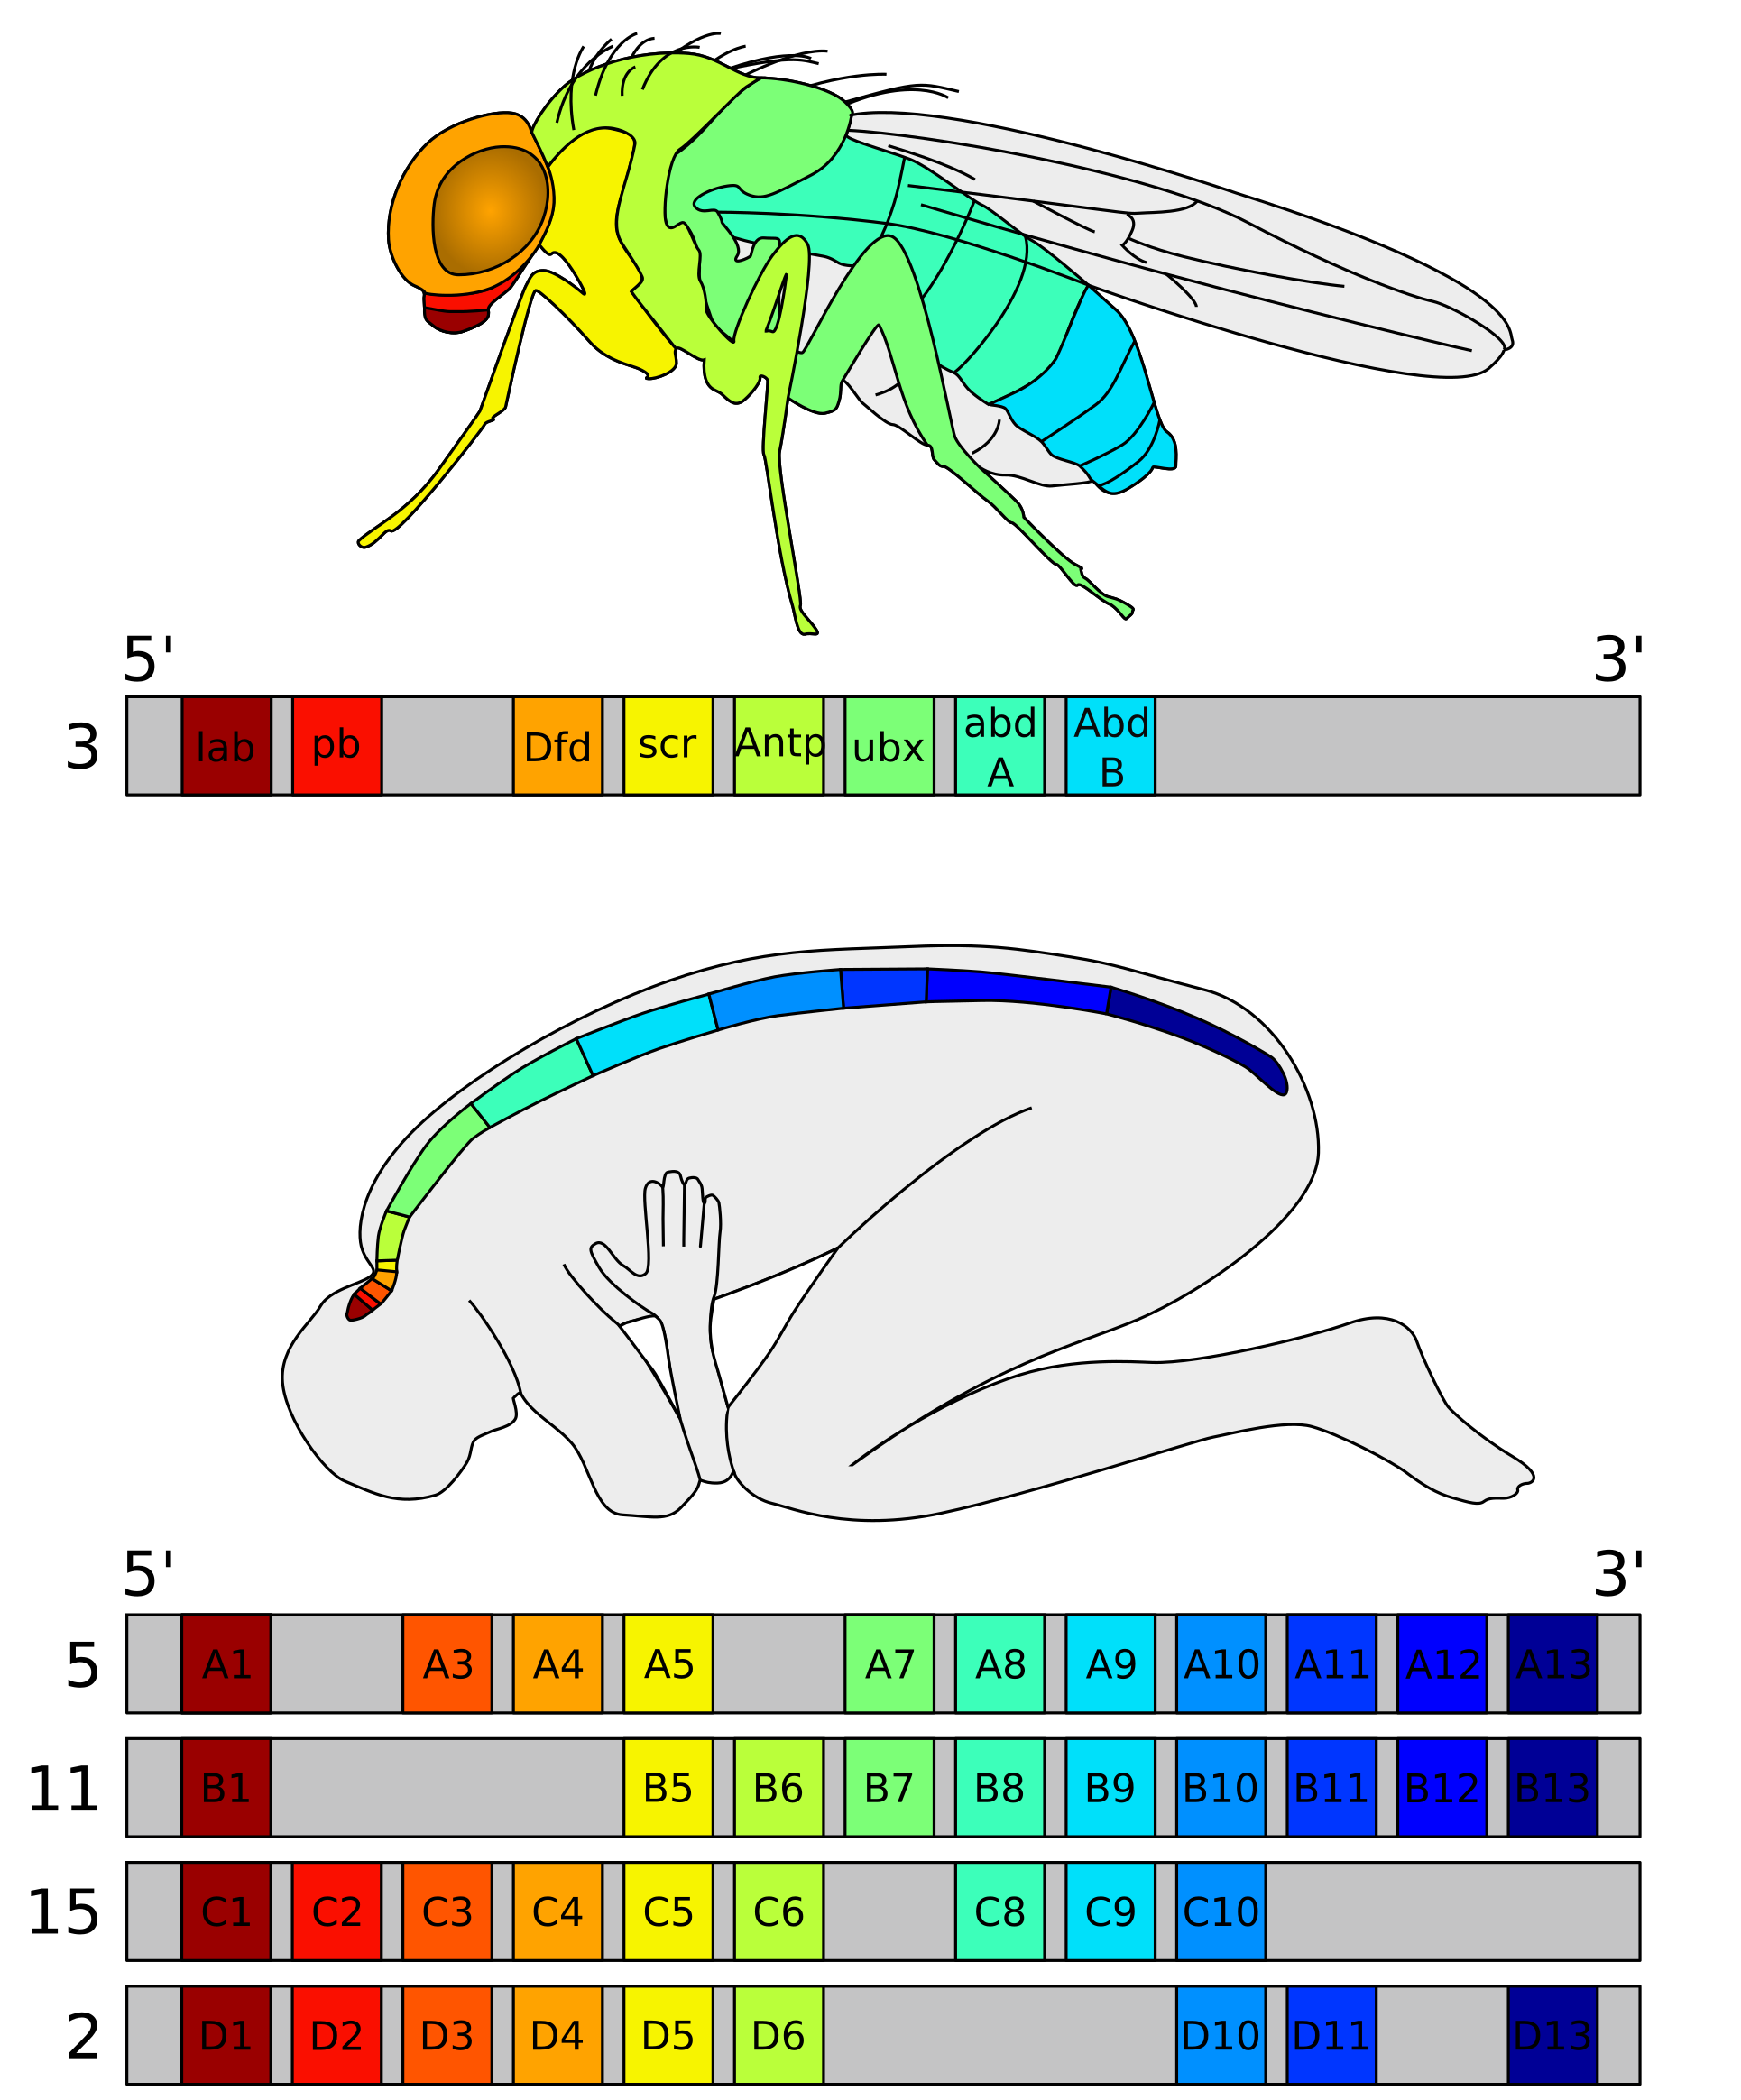
\includegraphics[width=\linewidth]{ch.introduction/imgs/hox.png}
    \caption{The genomic ordering of HOX genes in fruit fly and human, and their colinearity in expression. All the HOX genes for the fruit fly lay on chromosome 3. The human genome has had two genome duplications since the last common ancestor with fruit flies, so the HOX genes are spread over four chromosomes (5, 11, 15, and 2). Even though some HOX genes got lost on some chromosomes, their ordering has remained the same.}
    \label{fig:hox}
\end{figure}

Another remarkable family of transcription factors is the family of PAX transcription factors. While the HOX transcription factors are generally responsible for the anterior-posterior (head-to-tail) axis, the PAX transcription factors are involved in the development of structures like the eyes, ears, nervous system, and other organs. The most-studied of the family is the PAX6 transcription factor, which is involved in eye development and is highly conserved for bilateria (e.g. fruit flies, frogs, and humans). Injecting PAX6 into a developing frog embryo results in an extra eye on the spot of the injection\cite{Chow1999}.

The observation that single mutations can cause such large changes in body plans, in combination with the fact that the responsible genes are deeply conserved among species, shifted the way we think about evolution. Speciation does not have to happen through a combination of many small incremental mutations, but a few mutations, for instance, in the HOX or PAX genes, can cause major changes. This is now the basis of the scientific field of evo-devo.

\subsection{The hourglass model and the phylotypic stage}

Where the molecular observations of the HOX and PAX genes are a relatively recent addition to the field of evo-devo, the oldest observations in the field are based on the morphology (shape) of embryos. Ernst Haeckel has done the most famous and influential observations in the field of evo-devo in the 1800s\cite{haeckel1866}. Through a series of observations and drawings of the embryonic development of different vertebrates, Haeckel noticed a stage early in development where all vertebrates appear morphologically similar. This stage is now known as the phylotypic stage (see figure \ref{fig:haeckel_wide}). The Origin of Species, \textit{the} book by Charles Darwin in which he proposes the evolution theory, was only published a decade before these observations, and the idea of a scala naturæ (the ordering of species into higher and lower species) was still prevalent at that time. Haeckel thought his observations could unify the scala naturæ and the evolution theory, and came with a refinement of the recapitulation theory. Haeckel proposed that embryos of higher species consecutively develop from embryos of lower species into embryos of higher species. For example, a human embryo, which would be the highest and most developed species, would first develop into a fish embryo, then a reptile embryo, and finally into a mammalian embryo. This would explain why, for instance, gills and tails develop in human embryos, to then later disappear. The recapitulation theory unifies the scala naturæ with evolution, as the higher species are more evolved than the lower ones. Haeckel was a strong proponent of eugenics and proposed an ordering in human races, where the Germanic race, coincidentally the race Haeckel belongs to, was listed all the way at the top\cite{Levit2020}. The recapitulation theory was already controversial at the time it was proposed and is refuted by the contemporary scientific community. Nevertheless, the notion of a morphologically conserved stage early in development is prevalent to this day.

\hvFloat[doublePage,capWidth=n,
capPos=bottom,bindCorr=0.0cm]{figure}
{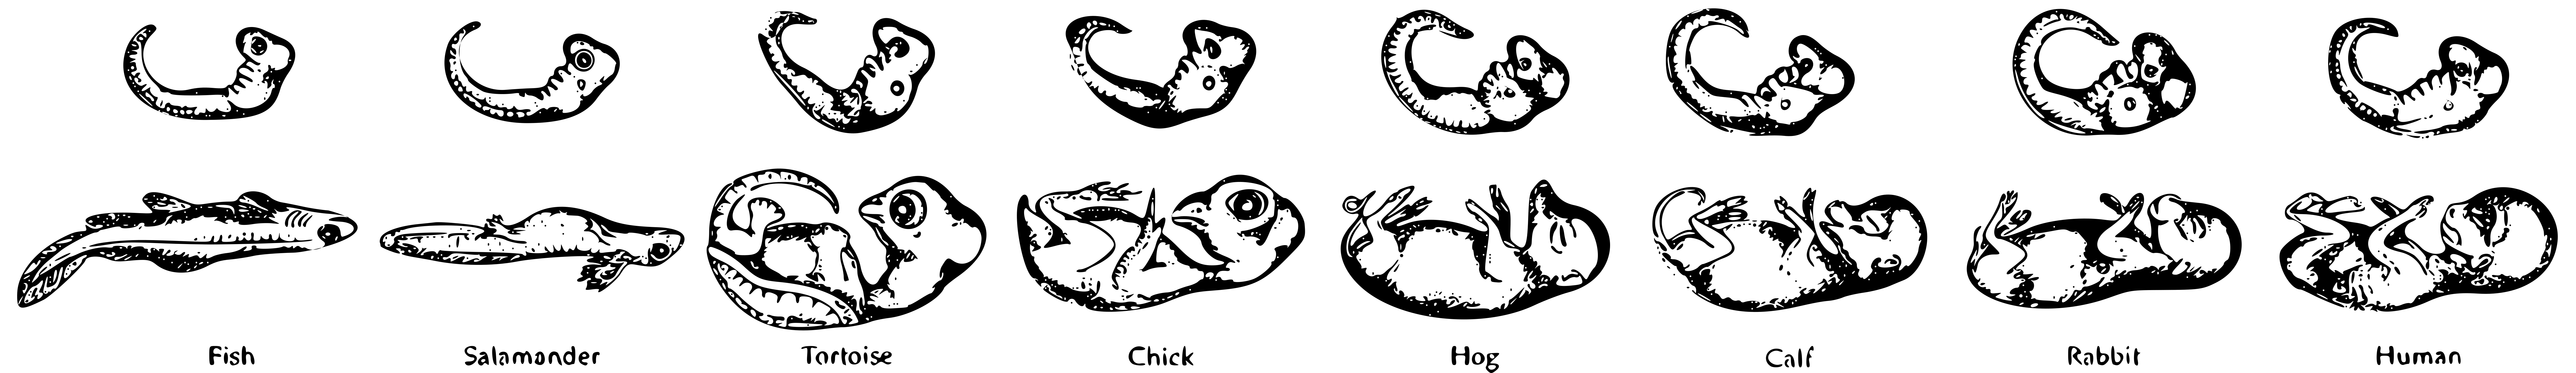
\includegraphics[width=2.2\textwidth]
{ch.introduction/imgs/haeckel_wide.png}}
[accessibility schematic overview]
{Adaptation of George Romanes's 1892 copy of Ernst Haeckel's embryo drawings. The upper row shows early embryos in the phylotypic stage, while the bottom row shows a later stage. Note how all the embryos appear similar in the phylotypic stage. Haeckel has been accused of fraud, amplifying the similarities at the phylotypic stage, with both supporters\cite{Richards2008} and opponents of his drawings\cite{Pennisi1997}}{fig:haeckel_wide}

In the same time period, Karl Ernst von Baer proposed an alternative theory of embryonic development. Von Baer was strongly opposed to Haeckel's recapitulation theory. He noted, for instance, that a yolk sac is present during bird embryonic development, but not for frog embryonic development. This is inconsistent with the recapitulation theory as frogs were considered a higher species than birds. Von Baer's opposing theory consisted of four main rules, or laws\cite{baer1828}. His first law, for instance, states that \textit{the more general characters of a large group appear earlier in the embryo than the more special characters}. This means that as an embryo develops, it first develops its oldest phylum-specific features, to then respectively develop its class, order, family, and species-specific features. Simply put, embryos of related species become increasingly diverse as development proceeds. Von Baer did not believe in the idea of a single common ancestor for all life on earth, as he believed the differences between some species, e.g. humans and sponges, to be too large to be bridged by evolution.

Even though the theories of Von Baer and Haeckel are dismissed by contemporary biologists, their observations of a morphologically conserved stage in development remain intriguing and have led to the formulation of the hourglass model of development. The hourglass model is based on the model proposed by Paul Medawar in 1954\cite{Medawar1954}. Medawar argues that somewhere mid-embryogenesis is the most morphologically conserved stage for vertebrates. This stage corresponds to Haeckel's phylotypic stage, but, different from Haeckel's recapitulation theory, different species are thought to be more diverse both before and after the mid-embryogenesis state. The phylotypic stage coincides with the formation of the basic body plan, so it is a popular hypothesis that HOX genes are responsible for this conserved stage. Recently, molecular evidence has been generated that gene expression between different species is most similar at the phylotypic stage \cite{Levin2016,marletaz2018,Mayshar2023,Liu2021,DomazetLoso2010,Irie2011,Kalinka2010,Piasecka2013,Uesaka2019}. This has led to the idea that the phylotypic stage is not just morphologically conserved, but also conserved on the level of gene expression and regulation. In chapter \textbf{TODO 1 and 2} I discuss the current statistical methods that estimate this molecular conservation, and by careful re-analysis, I demonstrate that the used methodology is biased. This in turn means that the conclusions the original authors draw about the phylotypic stage and the molecular hourglass model are unfounded. 

\section{Thesis overview}

This thesis focuses on the computational analysis of (evolutionary-) developmental processes. The current chapter (\textbf{chapter 1}) served as a general introduction to the scientific fields of computational genomics, gene regulation, and evolutionary development.  

In \textbf{chapter 2} I review the current computational approaches to model and understand gene regulatory networks in development. Current computational gene regulatory network inference methods perform poorly, and thus new approaches are needed. I highlight three recent developments for gene regulatory network inference which I expect to improve the power of these methods; multi-omics networks, single-cell data, and artificial neural networks. Multi-omics data partially solves the curse of dimensionality by constraining the problem and providing more data. Bulk sequencing measures the compound signal of multiple cell types. Single-cell sequencing, on the other hand, separates the signal per cell type, so cell-type-specific networks can be made and the data contains a purer signal. Artificial neural networks can model more complex gene-gene interactions than the current approaches. By combining these three approaches I expect future gene regulatory network inference methods to predict better networks.

In \textbf{chapter 3} I discuss the implementation of seq2science, a next-generation pre-processing workflow. Seq2science supports some of the most common assays, such as RNA-seq, ChIP-seq, and ATAC-seq, integrates with public databases, and reports an extensive quality control report. Seq2science has been tested on a wide array of different species and genome assemblies, and I show examples of common analyses that seq2science supports out of the box. Seq2science has an extensive user base\cite{Bright_2021,Xu_2020,Wester2021,SantosBarriopedro2021,Heuts2023,Tholen2023,Harlaar2022,LunaVelez2023,Neikes2023,Vierboom2021,Smits2020,Smits2022,Heuts2022,Rother2023,Ho2023,Sweep2023}, is downloaded over 50K times through Bioconda, and has more than 130 ``stars'' on GitHub.

In \textbf{chapter 4} I discuss the implementation of qnorm, a Python quantile normalization package. Quantile normalization is the process of fitting multiple distributions onto their average distribution. Python did not have a quantile normalization package yet, and the implementations on public fora about how to do quantile normalization did not resolve ties properly. Qnorm is fast-ish and scales to infinitely large tables as it can swap memory to disk.

In \textbf{chapter 5} I discuss the molecular basis of the phylotypic stage and its related models. I explain how the current definition and analyses of the phylotypic stage are ambiguous, as they do not distinguish within-species effects from between-species effects. For this reason, I propose that any study of the phylotypic stage includes at least a within-species comparison, a within-phylum comparison, and a between-phyla comparison. By applying these comparisons I find important flaws in the interpretation of previous results. I highlight three examples where the within-species pattern is enough to explain the between-species pattern. Moreover, I find that a supposed between-phyla effect, the mid-developmental transition, is a statistical artifact. Finally, I question the general validity of the current approaches to studying the phylotypic stage, as they are gross oversimplifications of the biological complexity during development.

\textbf{Chapter 6} is a short criticism of a quantitative study of morphological features in relation to the phylotypic stage. The original study finds support for an inverse hourglass model for mammalian embryonic development. However, with simulated data with no particular temporal conservation, I find nearly identical results. The methodology of the original study is biased towards the inverse hourglass, and as such I see no support for their claim of an inverse hourglass model of conservation.

In \textbf{chapter 7} (scepia)

Finally, in \textbf{chapter 8} I summarize and discuss the results described in this thesis, and give future perspectives on the field.

\chapter{Computational Approaches to Understand Transcription Regulation in Development}\thumbforchapter
\chaptermark{Computational Approaches to Understand Transcription Regulation in Development}
\chapterauthor{Maarten van der Sande*, Siebren Fr{\"o}lich*, Simon J. van Heeringen}
\newpage
\section{Abstract}

Gene regulatory networks (GRNs) serve as useful abstractions to understand transcriptional dynamics in developmental systems. Computational prediction of GRNs has been successfully applied to genome-wide gene expression measurements with the advent of microarrays and RNA-sequencing. However, these inferred networks are inaccurate and mostly based on correlative rather than causative interactions. In this review, we highlight three approaches that significantly impact GRN inference: (1) moving from one genome-wide functional modality, gene expression, to multi-omics, (2) single cell sequencing, to measure cell type-specific signals and predict context-specific GRNs, and (3) neural networks as flexible models. Together, these experimental and computational developments have the potential to significantly impact the quality of inferred GRNs. Ultimately, accurately modeling the regulatory interactions between transcription factors and their target genes will be essential to understand the role of transcription factors in driving developmental gene expression programs and to derive testable hypotheses for validation.

\section{Introduction}

Multicellular organisms develop from a single fertilized egg, guided by the genetic information encoded in the genome. Cell lineages diverge and form tissues and organs, based on the interplay between signaling pathways, biomechanical forces \cite{Mammoto_2012} and the regulation of gene expression programs \cite{Cameron_1987}. While development is controlled on many levels, transcription regulation is crucial \cite{Cooper2000}. To better understand these regulatory principles in development and evolution, it is essential to construct informative models of gene regulation.

Transcription is regulated by transcription factors (TFs) within the chromatin context \cite{Li_2004}. TFs bind the DNA either directly, mostly in a sequence-specific manner \cite{McMahon_1984}, or indirectly via other TFs \cite{Gord_n_2009}. They can recruit various other proteins, such as co-activators, RNA polymerase, chromatin remodelers and histone modifying enzymes, to remodel or stabilize the chromatin or to activate or repress transcription \cite{Chen_2021,Vaquerizas_2009}. In metazoans, TFs form up to 8\% of the known proteome \cite{Lambert_2018,Seb_Pedr_s_2018}, with DNA binding domains and affinities being highly conserved between metazoans \cite{Nitta_2015,Schmidt_2010,Villar_2014}. They bind specific DNA motifs that are clustered in relatively short cis-regulatory elements (CREs) that can be categorized as promoters, enhancers and insulators \cite{Levine_2005}. The exact function of an element depends on the combination of bound transcription factors, which is influenced by motif specificity, distance between motifs and motif directionality \cite{Avsec_2021,Brown_2007,Farley_2016,Wong_2020,Zeitlinger_2020}. Core regulatory modules and pathways involved in germ layer and axis formation are deeply conserved in metazoans \cite{Martindale_2005}.

A useful abstraction to study transcription regulation is a network of transcription factors and their target genes. This concept of a gene regulatory network (GRN) was introduced in 1969 by Roy Britten and Eric Davidson and later experimentally demonstrated in sea urchin embryos \cite{Britten_1969,Davidson_2002}. GRNs serve to predict the effect of transcription factor expression on gene transcription and to derive testable hypotheses for validation. More generally, they function to model cell type specification and differentiation in development as well as regulatory perturbations in disease. GRNs have been constructed, mostly based on experimental loss-of-function and gain-of-function studies, for a variety of developmental models. Examples include germ layer formation in echinoderms \cite{Cary_2020,Peter_2011,Saudemont_2010} and frogs \cite{Charney_2017,Koide_2005,Rankin_2011,Sinner_2006}, neural crest formation \cite{Lukoseviciute_2018,Williams_2019}, the Drosophila gap gene network \cite{Jaeger_2010} and hematopoietic development \cite{Kueh_2011,Pimanda_2010,Singh_2014}. However, experimental elucidation of a limited number of interactions is hard to scale. Regulatory interactions are highly context-specific \cite{Farley_2016,Ryan_2019} and most remain unknown \cite{Vaquerizas_2009,2012}.

Computational inference of genome-wide GRNs was made possible with the advent of expression microarrays. Expression levels between transcription factors and their target genes tend to correlate \cite{Ideker_2001} and genes with similar mRNA expression patterns are more likely to be regulated by a common transcription factor \cite{Allocco_2004,Eisen_1998}. This led to the conception of gene co-expression networks, where functional connections between genes are inferred by expression pattern similarity. WGCNA \cite{Zhang_2005} and ARACNe \cite{Margolin_2006} were among the first gene co-expression-based tools and remain popular. Presently, a multitude of GRN inference methods exists. Reviews on the technical details can be found here \cite{Levine_2005,Chasman_2017,Delgado_2019,Mercatelli_2020}. Recent advances in experimental and computational techniques means that GRN inference has progressed beyond simple co-expression. In this review, we will highlight three approaches that have the potential to significantly impact GRN modeling: (1) moving from one modality, gene expression, to multi-omics, (2) single cell sequencing for cell type-specific signal and (3) neural networks as flexible gene regulatory models (Fig. \ref{fig:compapproach}).

\begin{figure}
	\centering
	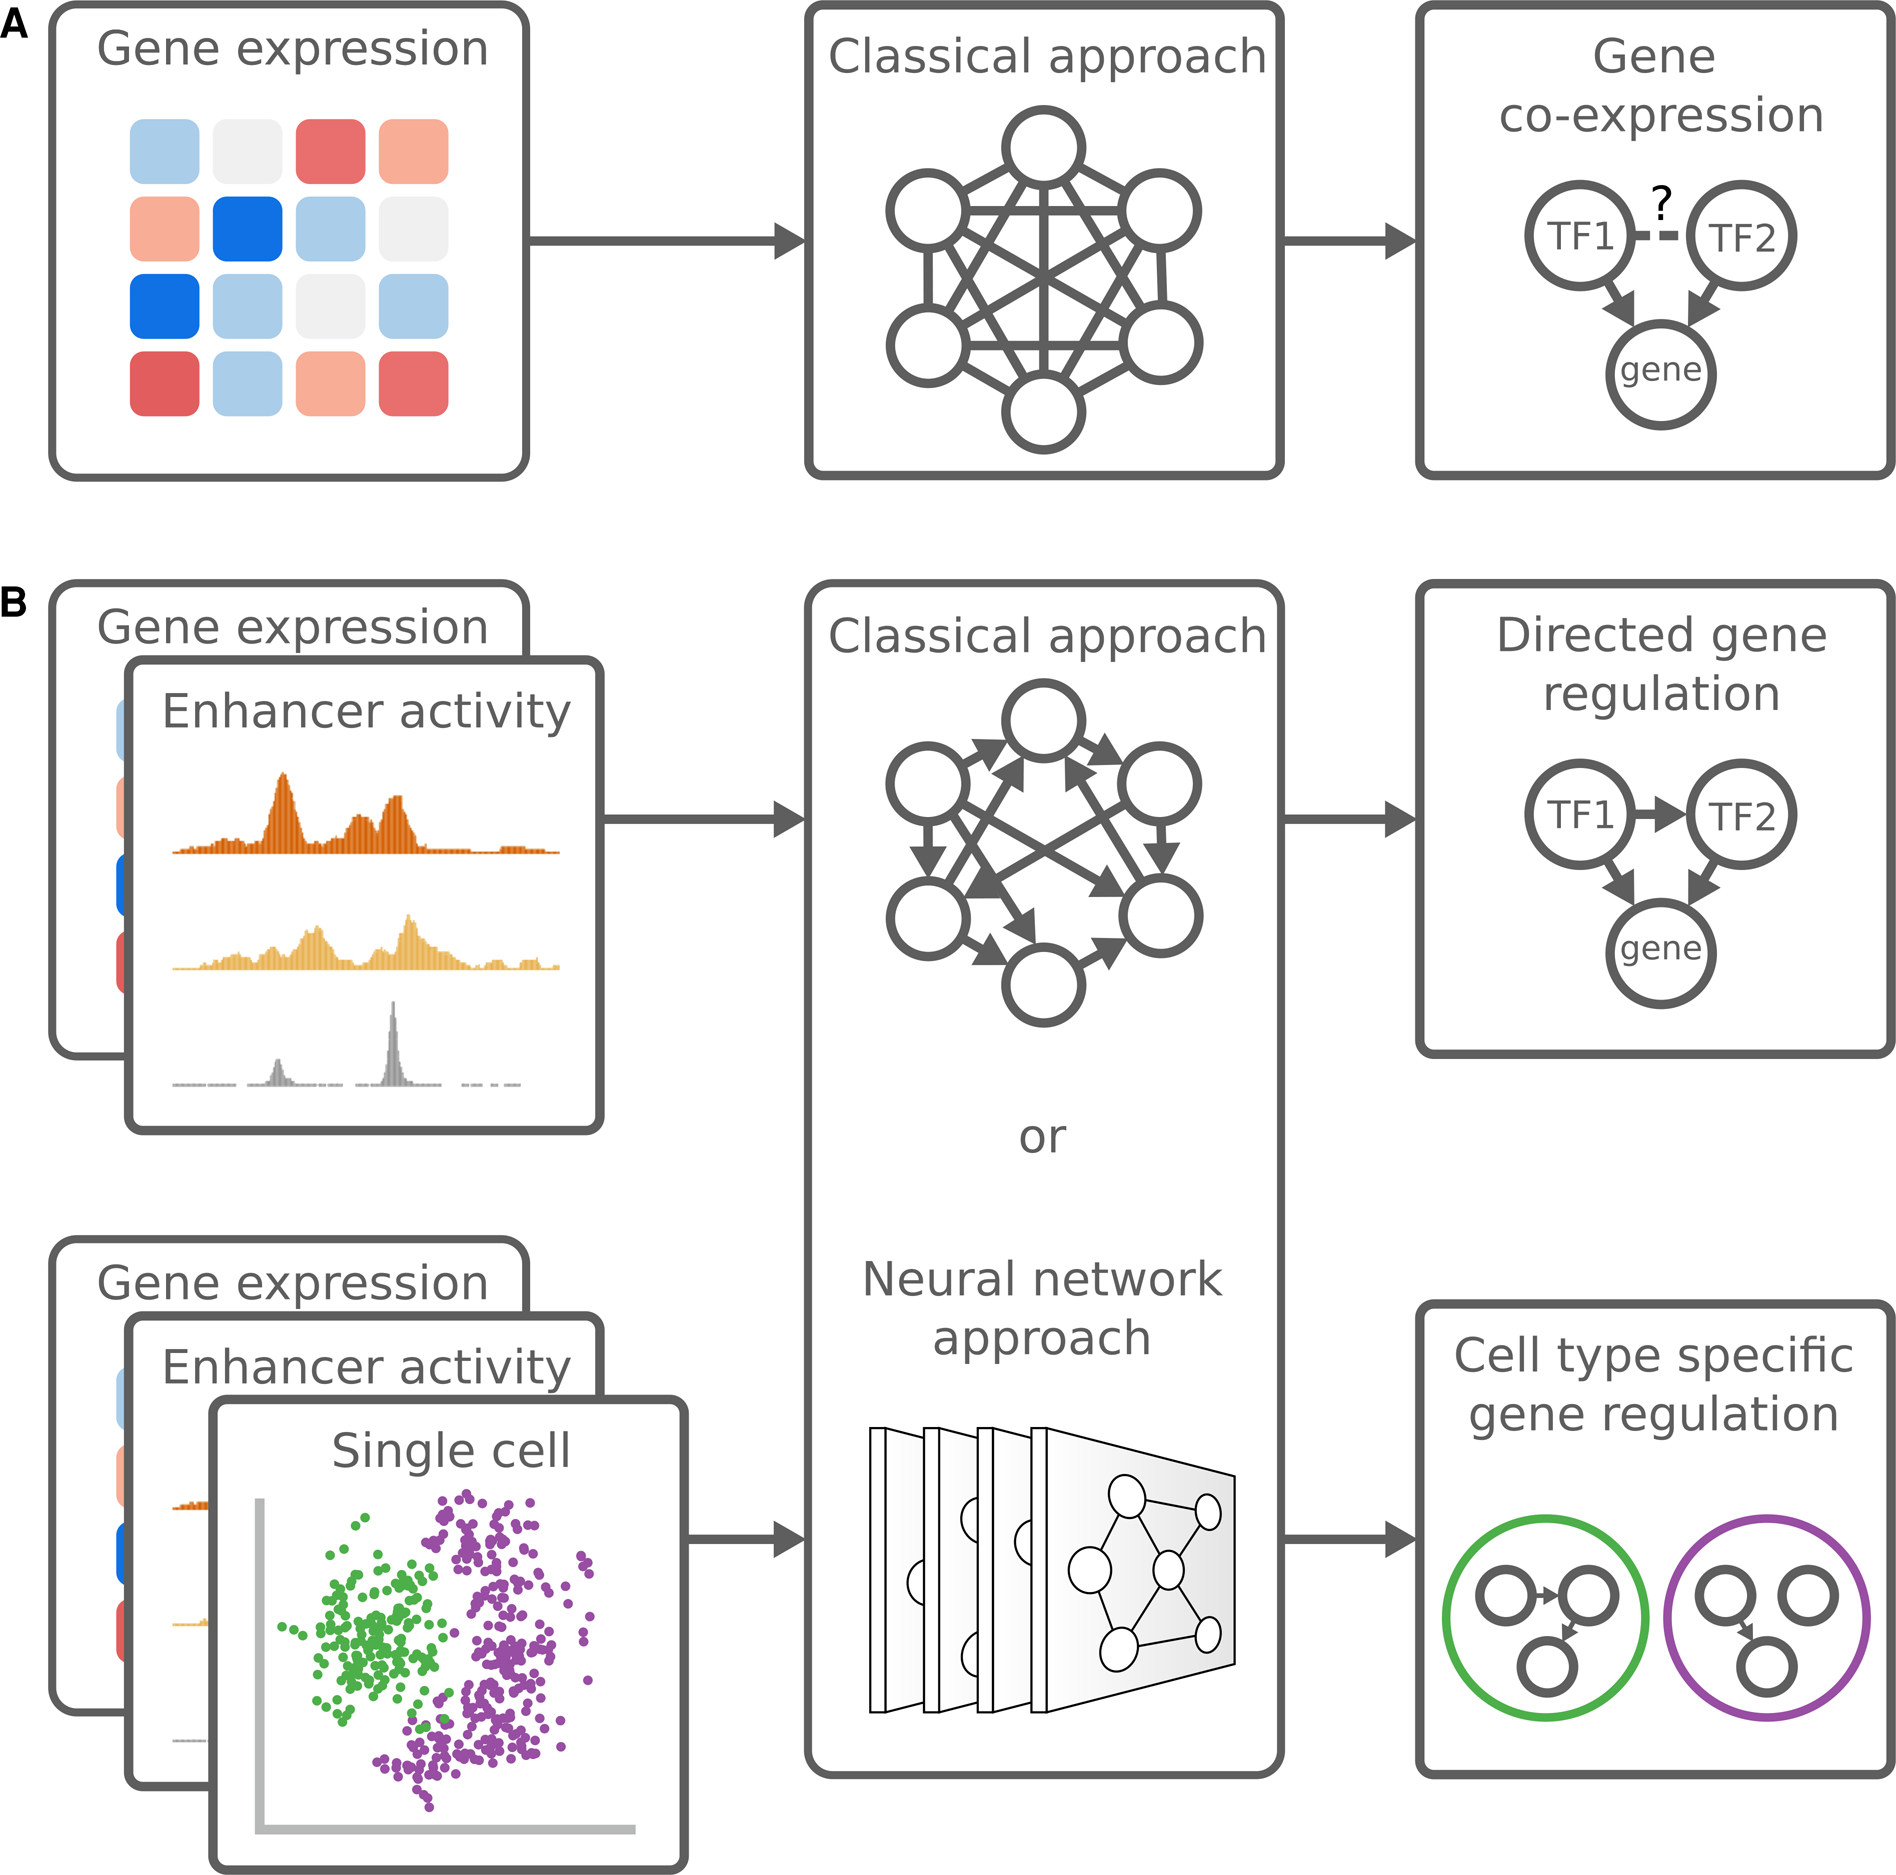
\includegraphics[width=0.9\textwidth]{ch.compapproach/images/compapproach.png}
	\caption{\label{fig:compapproach}\textbf{Schematic overview of different gene regulatory network inference approaches.} \textbf{(A)} Classical approaches, \textit{e.g.} correlation, regression or mutual information, can be applied on gene expression data to generate undirected co-expression networks. With prior knowledge about TFs the directionality between TF and target gene can be inferred, however, the directionality between two TFs cannot be established. \textbf{(B)} More recent approaches combine multiple types of genome-wide functional data (multi-omics), with either a classical approach or neural networks to identify directed gene regulatory networks. Single cell sequencing allows for the identification of cell type specific regulatory networks.}
\end{figure}

\section{Multi-omics to capture gene regulation}

Gene regulation by TFs is mediated through CREs including promoters and enhancers. By incorporating TF binding at enhancers, regulatory networks can be constrained by direct, causal relationships. Ideally, binding of TFs would be determined experimentally with chromatin immunoprecipitation followed by sequencing (ChIP-seq) \cite{Robertson_2007} or related techniques \cite{He_2015,Rhee_2011,Kaya_Okur_2019}. While large compendia of TF binding profiles in different cell types have been collected for humans \cite{2012}, this effort remains unfeasible for less well-studied organisms, including most developmental model systems. With sufficient training data, TF binding can be computationally imputed \cite{Keilwagen_2019,Li_2018,Quang_2019,Chen_2021,Mariani_2020,Li_2021,Bruse_2018,Schreiber_2020,Cheng2022,Behjati_Ardakani_2019,https://doi.org/10.48550/arxiv.2112.07571,Yi_2022,Pap_2021,Karimzadeh_2022,Koo_2020,https://doi.org/10.7303/syn6131484}, however, this does not necessarily generalize across species \cite{Cochran_2022}. As a result, most current approaches use relatively simple models that combine experimentally measured CRE activity with TF binding motifs to computationally predict TF binding.

Putative CREs and their activity can be mapped genome-wide using chromatin accessibility assays, such as DNase I hypersensitive sites sequencing (DNAse-seq) \cite{Boyle_2008} and Assay for Transposase-Accessible Chromatin using sequencing (ATAC-seq) \cite{Buenrostro_2013}. The number of reads in an element can then be used as a measure for CRE activity in the experimental system \cite{Buenrostro_2015}. ATAC-seq especially has been widely applied in developmental model systems, as it is experimentally relatively straightforward \cite{Williams_2019,Seb_Pedr_s_2018,marletaz2018,Uesaka2019,P_lfy_2020,Shashikant_2018,Madgwick_2019,Esmaeili_2020,Bright_2021,Yang_2020}. The chromatin environment can supply additional information on CRE location, function and activity. For instance, the transcriptional co-activator p300 is a histone acetyltransferase and can acytelate lysine 27 of histone H3 (H3K27ac). ChIP-seq using antibodies specific to p300 or H3K27ac can therefore identify active enhancers and promoters \cite{Visel_2009,Creyghton2010}. Other histone modifications that can be linked to CRE activity include H3K4me1 (enhancers) and H3K4me3 (promoters) \cite{Heintzman_2007}.

CRE activity is determined by (in)direct binding of several TFs \cite{Simeone_1988,Mitchell_1989}. Therefore, characterizing TF binding at enhancers can identify their relative importance to the function of an enhancer. One approach to infer TF binding from genome-wide DNA accessibility is digital genomic footprinting \cite{Hesselberth_2009}, which has been used to directly infer GRNs \cite{Neph_2012,Neph_2012}. However, sequence bias of the enzymes needs to be taken into account and TFs with more dynamic binding kinetics, such as some nuclear receptors, are not detected by footprint analysis \cite{He_2013,Sung_2016,Sung_2014}. Regardless, footprint analysis using cleavage bias correction can still be informative, especially in differential conditions \cite{Li_2019,Bentsen_2020}. A more routinely applied approach is to combine TF binding probabilities derived from TF motif scores with DNA accessibility. In some approaches, these are used as priors or constraints on network topology, where the network is inferred from gene expression measurements \cite{Miraldi_2019,Siahpirani_2016,Sonawane_2021}. In alternative approaches, TF motif scores and accessibility are combined with RNA expression using regression models or co-variation of accessibility and expression \cite{Madsen_2017,Kamal_2021,Schmidt_2018,Xu_2020,Ghaffari_2021,Vijayabaskar_2019}.

Enhancers regulate transcription via context-dependent enhancer-promoter interactions \cite{Levine_2010}, usually within a transcriptionally active domain \cite{Nora_2012}. Combined with TF binding data, these interactions allow for the inference of directed GRNs. Enhancer-promoter interactions can be identified experimentally with Chromatin Conformation Capture techniques \cite{Dekker_2002,Lieberman_Aiden_2009,Mifsud_2015}, although this is still uncommon in non-model systems. Inferring interaction between enhancers to target genes is an active field of research. The most commonly used heuristic is to link enhancers to the nearest gene. However, this heuristic is often still incorrect \cite{Sanyal_2012,Li_2012}. Accuracy can be improved by combining enhancer to gene distance with TF-target gene co-expression \cite{Marbach_2016}. Finally, Activity-by-Contact based models significantly outperform the nearest gene heuristic by using enhancer to gene distance and enhancer activity \cite{Fulco_2019}.

By combining gene expression data with at least one source of enhancer data (\textit{e.g.} accessibility or interaction data), directed regulatory networks may be inferred with significantly higher accuracy compared with traditional co-expression approaches \cite{Xu_2020,Mercatelli_2020,Glass_2013}. Not only does the combined approach filter out spurious interactions and add causality, but it also reduces the biases introduced by singular approaches. Therefore, we believe that the use of multiple omics will become dominant in all modalities of GRN inference approaches.

\section{Single cell sequencing for cell type specific regulation}

Developmental transcription regulation has mainly been studied by either in situ hybridization \cite{Jensen_2014}, which maps the spatial distribution of gene expression of a small set of genes, or bulk gene expression studies \cite{Wang_2009}. The latter measures the whole transcriptome as a compound signal of all the different cells present in the sample. Single cell sequencing is a fast developing technique to measure the gene expression of individual cells separately, with newer techniques even capable of tagging cells to their spatial coordinates \cite{Longo_2021,Borm_2022}. These techniques increase the number of measurements from a handful to several (tens to hundreds of) thousands. This substantial increase in data allows for interesting new ways of GRN inference, but poses new challenges as well.

The output of a single cell experiment generally consists of count tables containing several thousands of cells with low coverage, \textit{e.g.} only a few thousand of measured transcripts per cell. The low coverage makes the detection of relations between lowly expressed genes difficult. Although it is possible to artificially increase the sequencing depth by simulation (imputation), this does not seem to improve GRN inference \cite{Ly_2022,McCalla_2021}. Furthermore, it is important to note that cells are repeated measures \cite{Zimmerman_2021}, meaning that the cells come from the same environmental and genetic background, which breaks most statistical assumptions. Computationally clustering related cells, called pseudobulk or meta-cells \cite{Baran_2019}, and using their combined signal solves the issues of low coverage and repeated measures, and still yields cell-type specific signals.

Since fundamentally there are small differences between bulk and pseudobulk data, it is not uncommon to apply bulk GRN inference approaches, such as gene co-expression, ARACNE \cite{Margolin_2006} and GENIE3 \cite{Huynh_Thu_2010}, to pseudobulk data without much adjustment. The large number of cells, however, allows for specialized single cell GRN approaches. These include mutual information in combination with partial information decomposition \cite{Chan_2017}, gene coexpression \cite{Aibar_2017}, self-organizing maps \cite{Jansen_2019}, or a combination of single cell RNA-seq and single cell ATAC-seq coexpression and/or bayesian ridge regression \cite{Gonz_lez_Blas_2022,Jiang_2021,Kamimoto_2020}. Other approaches first order cells by their inferred temporal ordering and then infer the gene-gene relations on this pseudotime, with the assumption that these orderings, also called trajectories, represent cell lineages \cite{Packer_2019}. Pseudotime can be estimated by simply following the first principal component, or finding the minimal spanning tree between clusters \cite{Wolf_2019}, where more advanced methods smoothen the tree \cite{Qiu_2017,Street_2018}. A downside of these techniques is that they can not infer the directionality of the relationships. To computationally obtain this directionality, the ratio between spliced and unspliced transcripts per gene can be used as a proxy for whether or not a gene is actively transcribed. By applying this logic across all genes and all cells, one can infer a vector field of velocities of cells which then can be used to get a temporal cell ordering with a start and end \cite{Bergen_2020,La_Manno_2018}. These orderings then allow for inferring ordinary differential equations \cite{Aubin_Frankowski_2020,Matsumoto_2017}, Granger causality \cite{Deshpande_2022,Papili_Gao_2017,Qiu_2020}, boolean networks \cite{Woodhouse_2018} or autoregressive models \cite{Sanchez_Castillo_2017}. Most of these methods assume Gaussian noise for gene expression, even though transcription occurs in bursts \cite{Chubb_2006,Larsson_2019}, a phenomenon that can only be captured on a single cell level. These dynamics can be modeled as a Markov process including transcriptional bursting and degradation \cite{Ventre_2022}. Theoretically these mechanistic models could be great tools for hypothesis generation, but more work is needed to prove their practical usefulness. Even though the aforementioned GRN inference methods were developed for single cell data specifically, many fail to show consistent improvement over methods that were developed for bulk data, and are seemingly barely any better than purely random models \cite{McCalla_2021,Chen_2018,Pratapa_2020}. Moreover, the added complexity and number of cells leads to computational scaling issues, with some methods taking several days to weeks to finish \cite{McCalla_2021}.

Single cell sequencing has the advantage that it disentangles the composite signal present in all biological tissues. The increased number of measurements allows for more complex GRN definitions and inference. Finally, it allows for the inference of fine grained temporal orderings necessary for GRN inference. Even though single cell GRN inference methods have not yet brought the improvements over bulk methods we hoped for, we still expect single cell GRN inference to become the new standard of the field.

\section{Neural networks as flexible gene regulatory models}

Computational inference of a GRN depends on a lot of implicit assumptions. For example, a common assumption is that the relationship between genes is additive, which means that the effect on a gene equals the sum of the effects of two regulators separately, but in reality, gene-gene relationships are more complex and for example can include multiplicative effects \cite{Kim_2021}. A type of model that requires little explicit specification about the possible relationships in the data, but automatically learns these relationships, is an Artificial Neural Network (ANN). ANNs have been successfully applied in a variety of settings, with famously complex problems such as protein folding \cite{Jumper_2021}, image recognition \cite{Krizhevsky2017}, and the board game Go \cite{Silver_2016}. The successes of ANNs in these unrelated fields show great promise for application in the field of gene regulatory inference.

Just like GRNs, ANNs consist of nodes and edges. Each edge multiplies the signal from the previous node to the next, and by applying a function to the sum of all the incoming edges the value in the next node is calculated. By adding multiple layers of nodes in between the in- and output nodes (this is where the term deep neural network comes from), a network is formed that is capable of learning more and more complex interactions. Learning happens by giving the model examples of input data and expected output, and based on this information the model iteratively updates (learns) its edge weights. After training, hypotheses can easily be tested by systematically querying the model for the predicted effect of certain changes. See \cite{Eraslan_2019} for an excellent review on the topic applied to genomics.

ANNs in genomics were first applied to predict the output of a genomic assay, for instance, histone modifications in a certain cell type, by using only the DNA sequence as input. Early models showed that convolutional neural networks are capable of predicting functional effects of noncoding variants from short (10–1000 bp) genomic sequences alone \cite{Alipanahi_2015,Zhou_2015}. These types of models can be used to discover composite motifs and periodic binding \cite{Avsec_2021}. Additionally, these models are capable of learning complex and distal biological relations, as increasing the input sequence to 131 kb still improves accuracy \cite{Kelley_2018}.

Whereas ANNs in genomics have mainly been popularized on sequence data, adoption for GRN inference has been relatively slow. Different approaches consist of self-organizing maps \cite{Jansen_2019}, variational autoencoders \cite{Shu_2021}, extreme learning machines \cite{Rubiolo_2017}, or graph convolutional neural networks \cite{https://doi.org/10.48550/arxiv.1806.06975,Wang_2020}. Even though these networks differ in architectural designs, they all report higher levels of accuracy over non-ANN approaches. However, without independent benchmark studies, it is hard to verify these results.

The main strength of ANNs is that they can approximate any continuous relationship in the data \cite{Cybenko_1989,Hornik_1989}, with the downside that large amounts of training data are required. This makes the combination of single cell sequencing and ANNs promising, as current single cell GRN inference approaches have scaling issues \cite{McCalla_2021} and ANNs train relatively fast with the use of GPUs (graphics cards). Fundamentally, understanding how ANNs work is, however, much harder than understanding the classical models typically used for GRN inference. This causes ANNs to be met with skepticism and the persistent misconception that ANNs only function as a black box for predictions and its logic can not be interpreted \cite{Zhang_2021}. We expect ANNs to become commonplace in the field of GRN inference due to their successes in other fields, ease of implementation with high-level programming libraries \cite{chollet2015keras,https://doi.org/10.48550/arxiv.1912.01703}, and availability of sufficient training data due to single cell sequencing.

\section{Discussion}

Traditional GRNs, mostly based on gene co-expression, have so far served as a useful abstraction to understand regulatory dynamics in developmental systems. However, the way GRNs are currently derived suffers from two fundamental problems. First, the classic GRN that describes TF to target gene relations remains a simplified model and, by design, cannot properly reflect the full complexity of gene regulation. In addition, they are mostly based on mRNA expression as a measure of protein expression, even though this relation is not always linear \cite{de_Sousa_Abreu_2009}. In addition, any other types of regulation between transcript and protein product, such as mRNA degradation and post-translational modification, are usually ignored. Second, experiments generally have more features (\textit{i.e.} genes measured) than samples which is also known as ‘the curse of dimensionality'. In this underdetermined system, many different models can potentially fit to the data, and it is both practically and theoretically impossible to identify the correct model with certainty \cite{Krishnan_2007}. It then should not come as a surprise that benchmarks consistently demonstrate that the quality of the inferred GRNs is low \cite{Chen_2018,Pratapa_2020,Cokelaer_2016,dream,Guo_2017,Marbach_2012,STOLOVITZKY_2007}. Based on these observations it is clear that our current approach to infer GRN is not sustainable and design changes are needed. Ultimately, we expect the field to move towards GRNs inferred from neural networks trained on single cell multi-omics data.

Having said that, it is not enough to just naively apply single cell multi-omics ANNs. By adding more modalities, and making GRNs more complex, networks become even more underdetermined. This is why most multi-omics approaches use the new modalities to prune the possible TF-target gene relations, which actually reduces the degrees of freedom \cite{Xu_2020,Aibar_2017,Jiang_2021,Kamimoto_2020}. Moreover, one can use time-series data to further prune TF-target gene interactions \cite{Zoppoli_2010}, although time-series multi-omics GRN inference tools are still relatively uncommon \cite{Ernst_2007,Schulz_2012,Ding_2018,Conard_2021}. In addition, computational methods such as regularization \cite{Buhlmann} and dropout \cite{srivastava14a} constrain the problem in such a way that you end up with the simplest fit out of likely possible fits. In addition, recent developments have made it possible to measure multiple modalities in the same cell, such as combined ATAC-seq and RNA-seq \cite{Ma_2020,Cao_2018,Chen_2019}, which offers new, exciting opportunities for combining single cell sequencing with multi-omics data. ANNs, finally, have been made relatively easy to implement, can learn any type of interaction, and make no assumptions about the data (such as normality), which makes them extremely powerful GRN tools. However, it is not yet clear what the optimal architecture is for these networks, and interpreting the learned network from the ANN remains difficult.

GRN inference has become a data science, and it is time that we start treating it as such. Integrating multiple omics, several thousands of cells, and training complex machine learning models requires specialized knowledge. Common mistakes, such as treating cells from the same sample as independent \cite{Zimmerman_2021}, double dipping \cite{https://doi.org/10.48550/arxiv.2012.02936}, and data leakage \cite{Schreiber_2020}, can be avoided by proper data science training, but are unfortunately still common. Comparing the quality of GRN inference methods requires standardized benchmarks with multiple datasets, preferably a mix of experimental data and simulated data \cite{Dibaeinia_2020,Li_2022,Ventre_2022}. Simulated data has the advantage that the ground truth is known which makes benchmarking straightforward, but has the clear disadvantage that the quality of simulated data depends on its assumptions and may actually not be representative of real biological data. The DREAM challenges \cite{Cokelaer_2016,dream} and BEELINE platform \cite{Pratapa_2020} are great examples, with predefined datasets and quality metrics. Only by measuring network accuracy in equal settings will it be possible to properly compare methods. It is however important to note that the goal of GRN inference is to gain mechanistic insights, as opposed to getting an optimal benchmark score, which makes fair comparison between approaches hard.

Altogether, we expect the field of transcription regulation in development to move towards increasingly multimodal GRN inference techniques to identify causal relations between genes. Single cell sequencing adds a cell type-specific precision which bulk sequencing can not provide. Finally, we expect a more widespread adoption of artificial neural networks as the field matures in technology and formal training, as these methods are inherently more powerful than previously used techniques.

\section{Perspectives}

\begin{itemize}
    \item Gene regulatory networks have served as powerful models to understand gene regulatory programs in development and disease. Amongst others, these networks have been applied to model developmental patterning, to identify relevant transcription factors for cell fate transitions and to characterize deregulated transcriptional programs in disease.
    \item We believe three relatively recent developments will impact the computational inference of GRNs. The combination of multiple data modalities, such as RNA expression and DNA accessibility, help to constrain GRN topology and to predict directed networks. Single cell sequencing will become the de facto standard, as it allows for cell type-specific models and is able to provide the high number of measurements that are needed. Finally, artificial neural networks have the capability to create flexible and powerful models of gene regulation, which will benefit efficient and accurate GRN inference.
    \item The developments outlined above have the potential to significantly improve GRN inference. To fully exploit these approaches we have to implement common data science practices, and develop community-driven benchmarks to consistently measure the performance of different techniques.
\end{itemize}

% \section{Competing Interests}

% The authors declare that there are no competing interests associated with the manuscript.

% \section{Funding}

% Netherlands Organization for Scientific Research [NWO grant 016.Vidi.189.081 to S.J.v.H.].

% \section{Author Contributions}

% \textbf{Maarten van der Sande}: writing — original draft and writing — review and editing. \textbf{Siebren Fr{\"o}lich}: writing — original draft and writing — review and editing. \textbf{Simon J. van Heeringen}: writing — review and editing, funding acquisition, and supervision.

% \chapter{Seq2science: an End-to-End Workflow for Functional Genomics Analysis}\thumbforchapter
% \chaptermark{Seq2science}
\chapterauthor{Maarten van der Sande*, Siebren Fr{\"o}lich*, Tilman Sch{\"a}fers, Jos Smits, Rebecca R. Snabel, Sybren Rinzema, Simon J. van Heeringen}
\newpage

\section{Abstract}

Sequencing databases contain enormous amounts of functional genomics data, making them an extensive resource for genome-scale analysis. Reanalyzing publicly available data, and integrating it with new, project-specific data sets, can be invaluable. With current technologies, genomic experiments have become feasible for virtually any species of interest. However, using and integrating this data comes with its challenges, such as standardized and reproducible analysis. Seq2science is a multi-purpose workflow that covers preprocessing, quality control, visualization, and analysis of functional genomics sequencing data. It facilitates the downloading of sequencing data from all major databases, including NCBI SRA, EBI ENA, DDBJ, GSA, and ENCODE. Furthermore, it automates the retrieval of any genome assembly available from Ensembl, NCBI, and UCSC. It has been tested on a variety of species, and includes diverse workflows such as ATAC-, RNA-, and ChIP-seq. It consists of both generic as well as advanced steps, such as differential gene expression or peak accessibility analysis and differential motif analysis. Seq2science is built on the Snakemake workflow language and thus can be run on a range of computing infrastructures. It is available at \url{https://github.com/vanheeringen-lab/seq2science}.

\section{Introduction}

The Sequence Read Archive (SRA) at NCBI currently holds over 36 petabytes of sequencing data, and this volume is growing rapidly \cite{srawebsite}. Due to the flexibility of using sequencing as a readout, a large variety of different assays are available, such as RNA-sequencing (RNA-seq) \cite{Nagalakshmi2008} for gene expression quantification, Chromatin Immunoprecipitation (ChIP) sequencing \cite{chipseq} to profile DNA-bound proteins and assay for transposase-accessible chromatin with sequencing (ATAC-seq) \cite{Buenrostro_2015} to determine DNA accessibility. This wealth of public data enables researchers to verify results, re-analyze data with novel techniques, and to combine and integrate datasets from different studies. However, processing these large amounts of data is a challenging and time-consuming task, even for researchers that are already familiar with high-throughput sequencing data processing details. To address this issue, various workflow systems have been developed, roughly categorized into three approaches: community-oriented workflow collections, multi-purpose workflows, and single-purpose workflows.

Community-oriented workflow collections enable multiple users to contribute workflows, as long as they conform to the established style and language of the community. Examples of community-based workflow collections include Galaxy \cite{galaxy}, Snakemake-Workflows \cite{snakemakeworkflows}, and nf-core \cite{nfcore}. These collections offer the advantage of supporting a wide range of workflows and assays, with an active community providing support. Multi-purpose workflows facilitate multiple highly consistent workflows and typically provide a single entry point for users. Examples include Snakepipes \cite{snakepipes}, ENCODE pipelines \cite{encode2023}, and CellRanger \cite{Zheng2017}. These workflows are designed to maintain consistency across different analyses, making it easier for users to learn and analyze the supported workflows. Single-purpose workflows are tailored to address specific problems, such as ARMOR for RNA-seq \cite{Orjuela2019} and PEPATAC to analyze ATAC-seq \cite{Smith2021}. The advantage of these workflows lies in their high level of specialization, focusing on particular tasks or analyses.

Although there is a choice of publicly available, published workflows, we found that these did not address all of our requirements. First, apart from some exceptions such as Galaxy, most workflows have not been specifically designed with public data in mind. This requires users to download and prepare the data in advance. While this is doable for small studies, it quickly becomes prohibitive for more large-scale analyses combining data from different studies. Additionally, many workflows have been primarily developed for, and tested on, human and/or mouse data. This limits their applicability to non-model species. It can be cumbersome to add new genomes and supporting gene and transcript annotation. Finally, workflows that do not actively encourage data exploration leave users susceptible to missing biases and failing to uncover concealed insights. Workflows should make sure to include a variety of quality control results and diagnostic plots, as it is essential to check the quality of the data. This includes, for instance, checking mapped data visually using a genome browser. 

To address these limitations, we have developed seq2science, a multi-purpose workflow that supports virtually all public sequencing databases, multiple sequencing assays, and any species of interest. Seq2science is capable of automatically downloading genome assemblies and raw sequencing data from a range of sources. It supports multiple read trimmers, aligners, peak callers, and quantification methods, and generates an extensive quality report and a fully configured UCSC trackhub. It currently supports bulk ChIP-, ATAC- and RNA-seq, downloading of FASTQ files, and a generic genomic alignment workflow. Installation is easy through the Conda package manager, and extensive \href{https://vanheeringen-lab.github.io/seq2science/}{documentation is available online}. Seq2science is designed to cater to both intermediate and advanced bioinformaticians. It serves as an accessible starting point for those with a basic grasp of bioinformatics concepts, thanks to its sensible default settings. Additionally, it offers a high degree of customization, making it appealing to advanced users who seek more tailored control over their analyses.

\section{Methods}

\subsection{Implementation}

Seq2science is built using Snakemake \cite{snakemake}, a portable and open-source workflow system, which divides a workflow into independent modules called rules. Each rule includes a piece of code, its expected output, and optional input requirements. This design allows rules to be linked together, with the output of one rule serving as the input for another. Snakemake automatically determines the order in which rules need to be executed and distributes these tasks across available resources. To ensure reproducibility, most rules are assigned a specific virtual environment using the Conda ecosystem \cite{anaconda} that is automatically installed at the start of a run.

\begin{figure}
	\centering
	
\includegraphics[width=\textwidth]{ch.seq2science/imgs/figure_overview.png}
	\caption{\label{fig:overview} \textbf{Schematic overview of seq2science}. Seq2science can conceptually be split into six parts: downloading of samples and genome assembly, trimming of reads, transcriptome/genome mapping, quality control, initial analysis, and the final output. For each part the corresponding supported tools are listed. }
\end{figure}

Seq2science requires two input files: a samples file and a configuration file. The samples file is a table containing a column of FASTQ files (or public identifiers for automatic downloading from any of the supported databases), a column with the assembly the FASTQ file must be mapped to, and optional additional metadata columns. Optional columns are the descriptive name of the samples, information about the relations between samples such as whether samples are technical and/or biological replicates, and other such details. The configuration file is a YAML file with configurable parameters. These include whether to execute certain steps, the options to use when executing rules, and the directories where the output will be stored. Detailed explanations for the samples file and configuration file are available in the online documentation, and examples of these files are in the Supplemental Information and available at Zenodo (\url{https://doi.org/10.5281/zenodo.8345208}).

\subsubsection{General overview}

Regardless of the chosen workflow, when seq2science is executed, it checks for the local availability of the genome assembly and sequencing reads (in FASTQ format). If the genome assembly or the reads are not found locally, seq2science will download them. Once the raw data is obtained, the FASTQ files are prepared for alignment. This involves  building a genome index and trimming the reads. The aligned reads are then duplicate-marked, filtered, and sorted according to the configuration settings. Nearly all workflows produce a set of indexed BAM (or optionally CRAM) files, an extensive quality control report, and a UCSC trackhub at this stage. The ATAC- and ChIP-seq workflows call peaks, and the output is stored and aggregated into a peak counts table. The RNA-seq workflow uses the specified quantifier to obtain raw gene counts and TPM tables. Optional differential gene expression, peak accessibility, and motif activity analyses are fully supported. Finally, a workflow explanation is generated with the parameters, version, and citation per tool which is also embedded in the QC report. For a schematic overview of the different steps and supported tools of seq2science see \autoref{fig:overview}. 

\subsubsection{Download-fastq}

The download-fastq workflow can retrieve FASTQ files from various databases: the European Nucleotide Archive (ENA) \cite{ENA}, Gene Expression Omnibus (GEO) \cite{GEO}, the Sequence Read Archive (SRA) \cite{Leinonen2010}, the DNA Data Bank of Japan (DDBJ) \cite{DDBJ}, the Genome Sequence Archive (GSA) \cite{GSA} and the ENCODE project \cite{Luo2019}, using their specific identifiers; ERX, ERR, GSM, SRX, SRR, DRX, DRR, CRX, ENCSR, or ENCFF numbers. The SRA, ENA, and DDBJ databases contain raw sequencing data that must be converted to FASTQ format, and they generally mirror each other in their content. EBI ENA, GSA, and ENCODE, however, store FASTQ files directly, so if a sample on the SRA or DDBJ is found to be mirrored on ENA by pysradb \cite{Choudhary2019}, seq2science will directly download FASTQ files from there, optionally using Aspera Connect (ascp), which is a high-speed transfer protocol developed by IBM. If the sample is not directly available in FASTQ format, seq2science uses the sra-toolkit \cite{Leinonen2010} to download the raw data and parallel-fastq-dump, a parallelized version of fastq-dump, to convert the data to FASTQ files.

\subsubsection{Alignment}

The alignment workflow in seq2science processes FASTQ files that are either already present on the device or are automatically obtained using the download-fastq workflow. If necessary, the workflow will also download a genome assembly FASTA file and corresponding gene annotation file using genomepy \cite{Frlich2023}. The FASTQ files are trimmed for quality and adapters using either TrimGalore \cite{trimgalore} or fastp \cite{Chen2018}, as specified by the user. The trimmed FASTQ files are then aligned to the genome using the selected mapper, such as bowtie2 \cite{bowtie2}, bwa-mem \cite{bwamem}, bwa-mem2 \cite{bwamem2}, HISAT2 \cite{hisat2}, minimap2 \cite{minimap2}, or STAR \cite{star}. The resulting BAM file is filtered based on criteria such as MAPQ value, duplicate status, or alignment in the ENCODE blacklist \cite{blacklist}. The filtered BAM file is then converted into a bigWig file and prepared for visualization in a UCSC trackhub \cite{trackhub} or, when the genome assembly is not hosted by UCSC, as an assembly hub. The filtered BAM file can optionally be stored as a CRAM file to save disk space. Quality checks are performed throughout the process using FastQC \cite{fastqc}, samtools \cite{samtools}, Picard \cite{picard}, and deepTools\cite{deeptools}, and the results are summarized in a MultiQC report\cite{Ewels2016}.

\subsubsection{ATAC- \& ChIP-seq}

The ATAC- and ChIP-seq workflows are identical in implementation, except that they are initialized with different default settings. They internally use the same rules as the alignment and download-fastq workflows, which means that they either start by downloading FASTQ files,  or analyze files that are already present. For the ATAC-seq workflow the aligned reads are by default Tn5 shifted \cite{Yan2020} and only reads with a maximum template length of 150 base pairs are kept. Peak calling is done on the filtered BAM files with either MACS2 \cite{Zhang2008} or genrich \cite{genrich}, with optionally specified control samples. Biological replicates can be combined either with the internal Fisher's method of either tool, or with IDR \cite{idr}. Peaks between conditions are combined when they fall within a certain range of each other with GimmeMotifs \cite{Bruse_2018} and a count table is made for all samples based on the number of reads in peaks. Optional differential peak analysis with DESeq2 \cite{deseq2}, or differential motif analysis with GimmeMotifs \cite{Bruse_2018} can be performed if selected. When doing a differential motif analysis, seq2science automatically converts the transcription factor gene names in the motif database into the (orthologous) gene names of the assembly used when a genome annotation is available. Additional QC is collected by deepTools \cite{deeptools}, ChIPseeker \cite{chipseeker}, and Subread \cite{subread}. See file S14 for a directed acyclic graph of all the steps involved with the ATAC- and ChIP-seq workflows.

\subsubsection{RNA-seq}

The RNA-seq workflow begins with the acquisition and processing of FASTQ files as described in the alignment and download-fastq workflows. Gene expression quantification can be based on either genomic alignment or transcript quantification, depending on the settings. For genomic alignment, reads are aligned to the genome with a splice-aware aligner (STAR \cite{star} or HISAT2 \cite{hisat2}). The output BAM files are filtered and have their duplicate reads marked. Gene expression quantification is then performed by assigning reads to genes, using HTSeq\cite{Anders2014} or featureCounts \cite{subread}. Ambiguous transcripts are minimized by providing the gene counting tools with the strandedness of each sample, which is inferred using RSeQC \cite{rseqc}. Additional gene-based TPM expression levels are generated using genomepy \cite{Frlich2023}, based on longest transcript lengths. For the gene quantification approach, transcript abundances are quantified using Salmon \cite{salmon} in mapping-based mode. To improve mapping accuracy, decoy sequences are generated as suggested by the Salmon documentation. The transcript abundances are aggregated to gene level using pytxi \cite{pytxi} or tximeta \cite{tximeta} and additionally converted to gene counts using genomepy \cite{Frlich2023}. 

Independent of the configured gene expression quantification approach, the workflow supports differential gene expression analysis with DESeq2 \cite{deseq2} with batch effect correction to integrate (multiple) datasets, and can prepare an exon count table for downstream use with DEXSeq \cite{dexseq}. Strand-specific bigWig files are generated for visualization in a UCSC trackhub. The trackhub configuration file is updated with strand information for ease of use. Additional quality control metrics specific to RNA-seq are obtained from DESeq2 \cite{deseq2} and dupRadar \cite{dupradar}. See Supplemental File S15 for a directed acyclic graph of all the steps involved with the RNA-seq workflow.

\section{Use Cases} % Optional - only if no new datasets are included

To briefly illustrate some of the capabilities of seq2science, we show how to use it to download publicly available FASTQ files, and finally show three example processing runs using public data.

\subsection{Downloading FASTQ files}

Downloading FASTQ files with seq2science has been made extremely easy. After installation of seq2science (see Supplemental File S1), all that needs to be provided is a tab-separated file with database identifiers. Seq2science currently supports identifiers for ENA, GEO, SRA, DDBJ, GSA, and ENCODE. For this example, we will download one FASTQ file from each database. To get started we need to initialize seq2science in the current directory:

\begin{minted}{text}
    seq2science init download-fastq
\end{minted}

After this initialization, we get a config and a samples file. The config file is practically empty as there is not much to configure for the download-fastq workflow. For this workflow, the relevant option is the directory where we want the samples to be downloaded.

\begin{table}[t]
    \hrule height 0.05cm  \vspace{0.01cm}
	\caption{\label{download.tsv}Example samples file for the download-fastq workflow. }
	\centering
    {\begin{tabular}{|l|l|l|l|l|l|}
    \hline
        sample \\  \hline
        ERX000401 \\ \hline
        ERR022487 \\ \hline
        GSM2811115 \\ \hline
        SRX257149 \\ \hline
        SRR800037 \\ \hline
        DRX029591 \\ \hline
        DRR032791 \\ \hline
        CRX269079 \\ \hline
        ENCSR535GFO \\ \hline
        ENCFF172MDS \\ \hline
    \end{tabular}}
\end{table}

We then edit the samples file and add the experiment (or run identifier) of each sample (\autoref{download.tsv}). Here we show a mixture of paired-end and single-end samples to highlight seq2science's ability to work with both data types. To download these samples all we now have to do is run seq2science:

\begin{minted}{text}
    seq2science run download-fastq --cores 8
\end{minted}

Seq2science will now start downloading our samples. Samples hosted on GSA, ENCODE, and ENA are downloaded directly as FASTQ file, whilst the samples not on ENA, ENCODE, or GSA first get downloaded as an intermediate SRA file which then gets converted into a FASTQ file. Even though we have specified the DRX and DRR samples by their DDBJ identifier, seq2science finds their ENA mirror if it exists and directly downloads those to save computational resources. At the end of this run, we end up with the corresponding FASTQ files for all ten samples.

\subsection{A map of cis-regulatory elements in zebrafish}

\begin{figure}
	\centering
	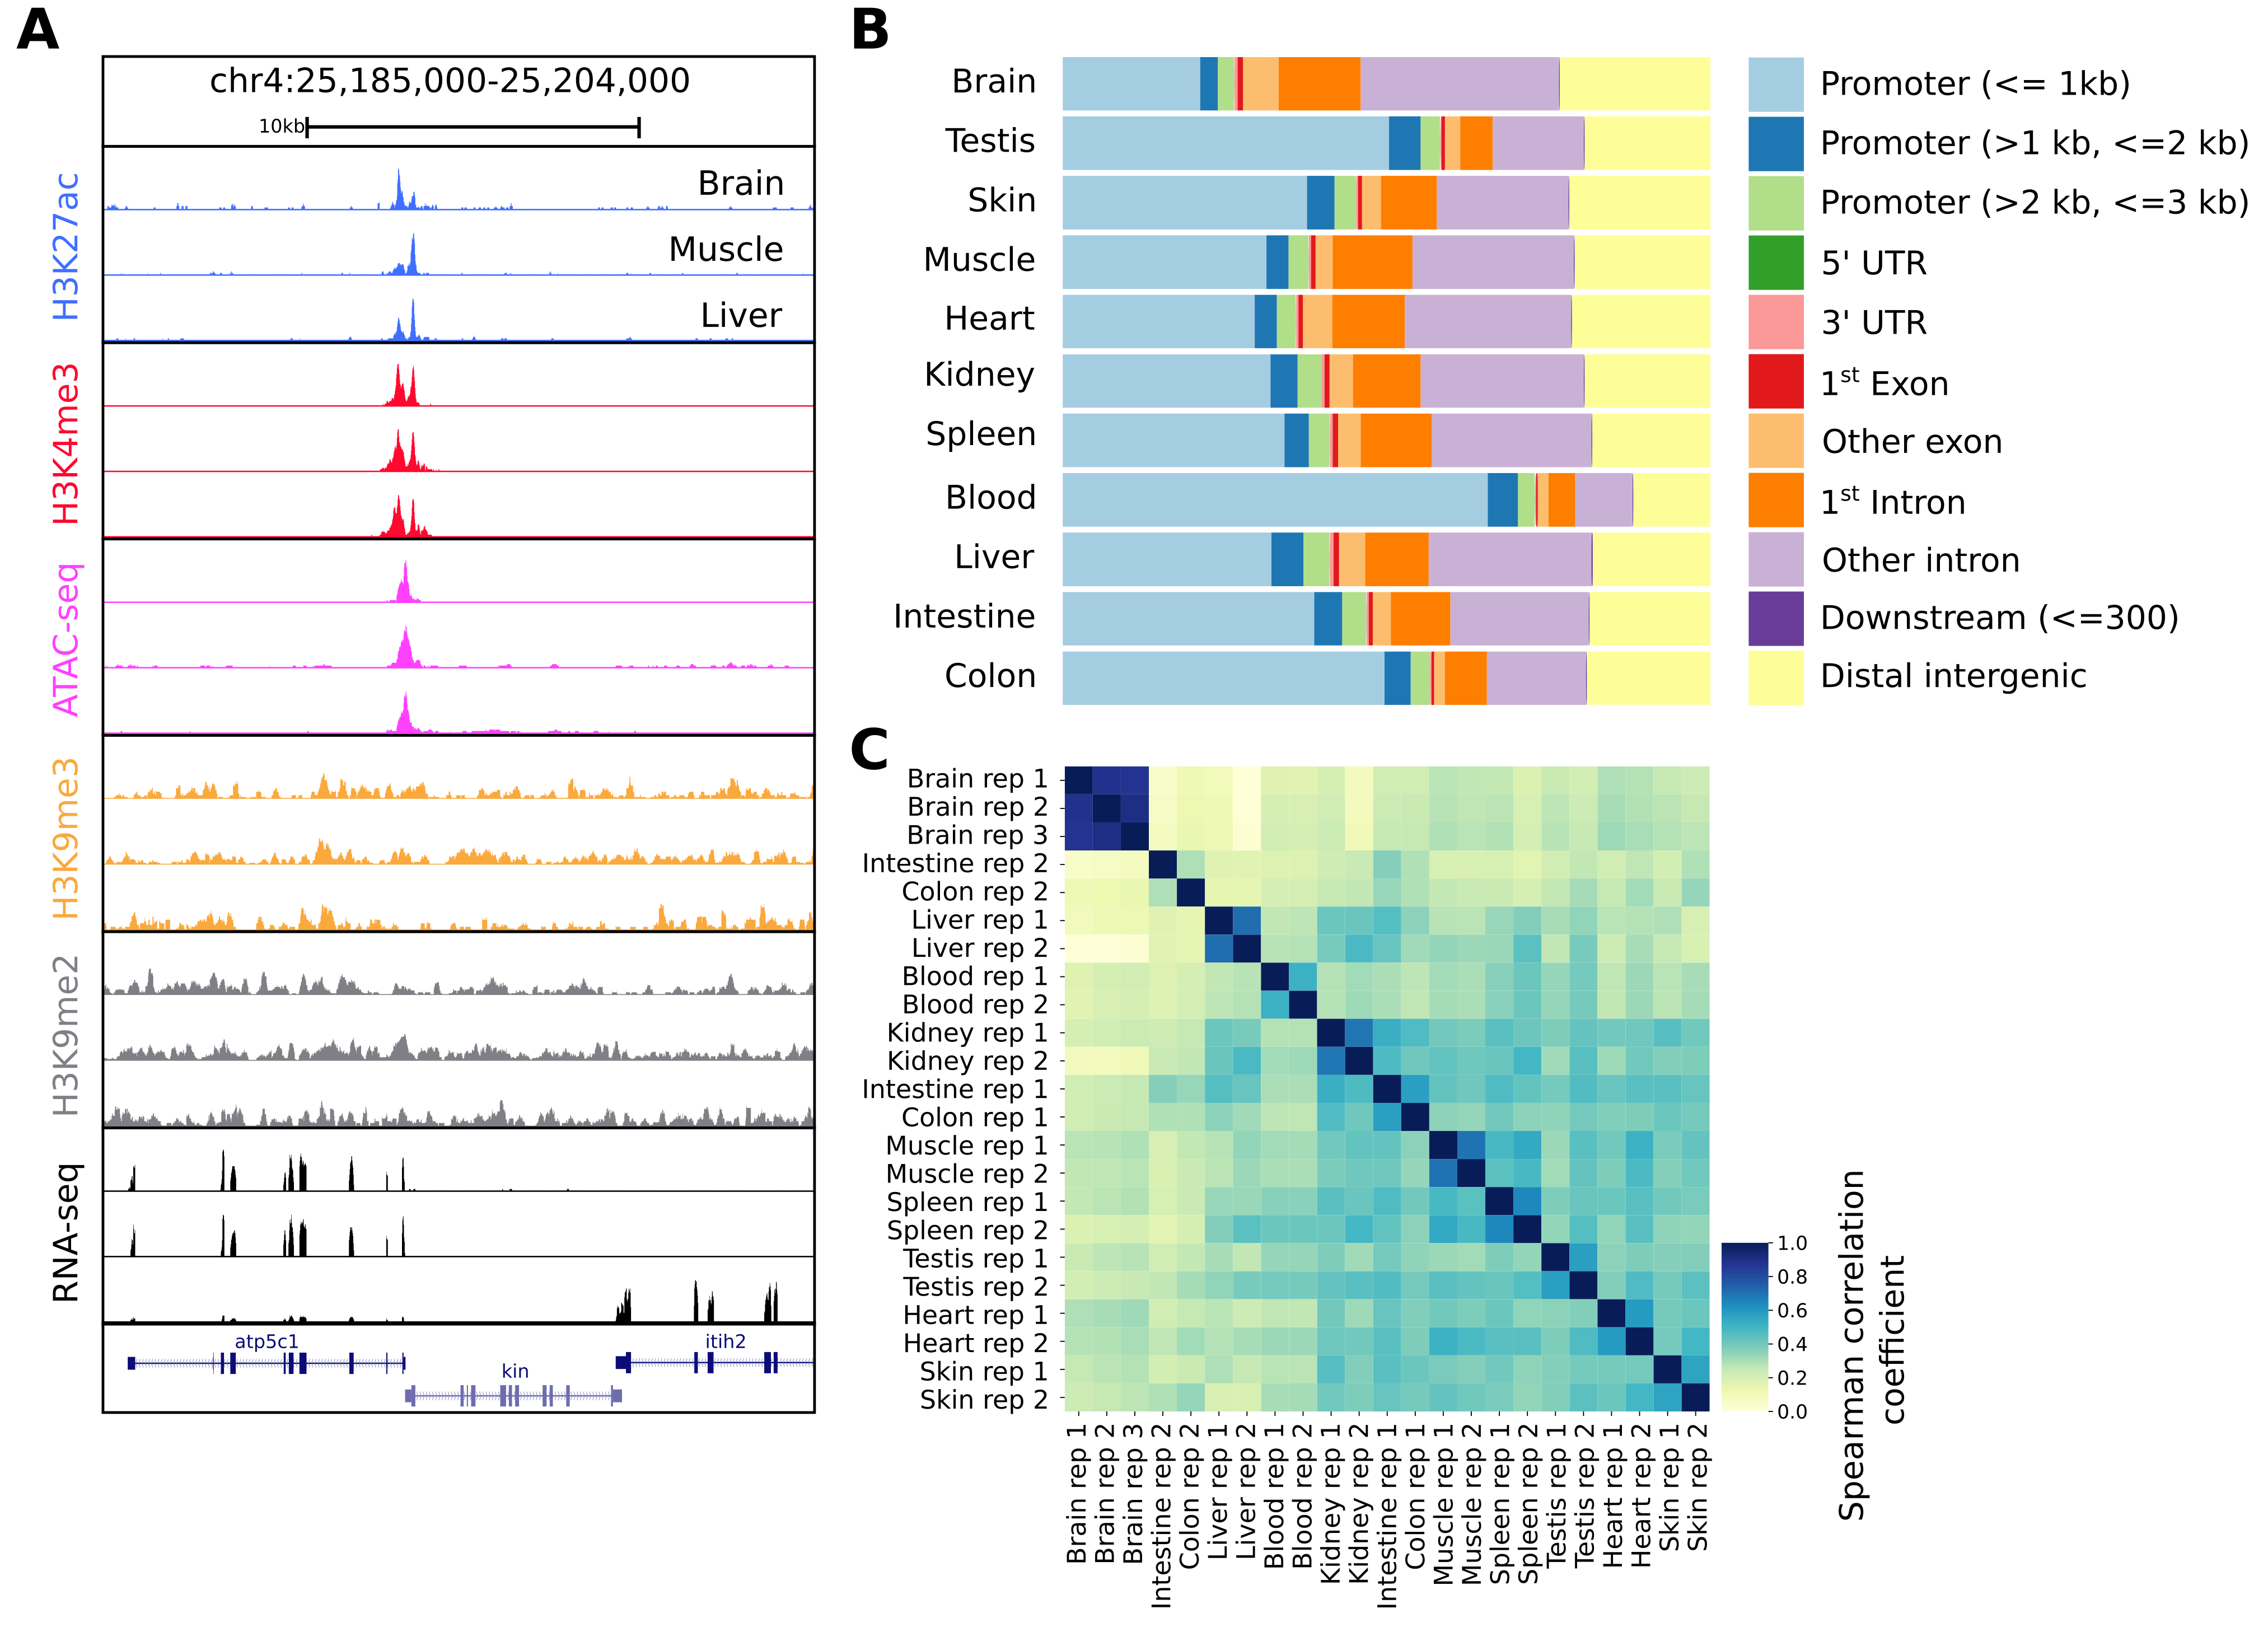
\includegraphics[width=1.0\textwidth]{ch.seq2science/imgs/zebrafish_fig1.png}
	\caption{\label{fig:zebrafish_fig1} \textbf{Snapshot of the UCSC trackhub and quality figures of seq2science}. \textbf{(A)} Fully configured UCSC trackhub generated by seq2science which highlights some of the supported assays. \textbf{(B)}  The fraction of ATAC-seq peaks predicted in each tissue and their genomic distribution, visualized by ChIPseeker. \textbf{(C)} Pairwise Spearman correlation coefficients of all the samples. }
\end{figure}

\begin{figure}
	\centering
	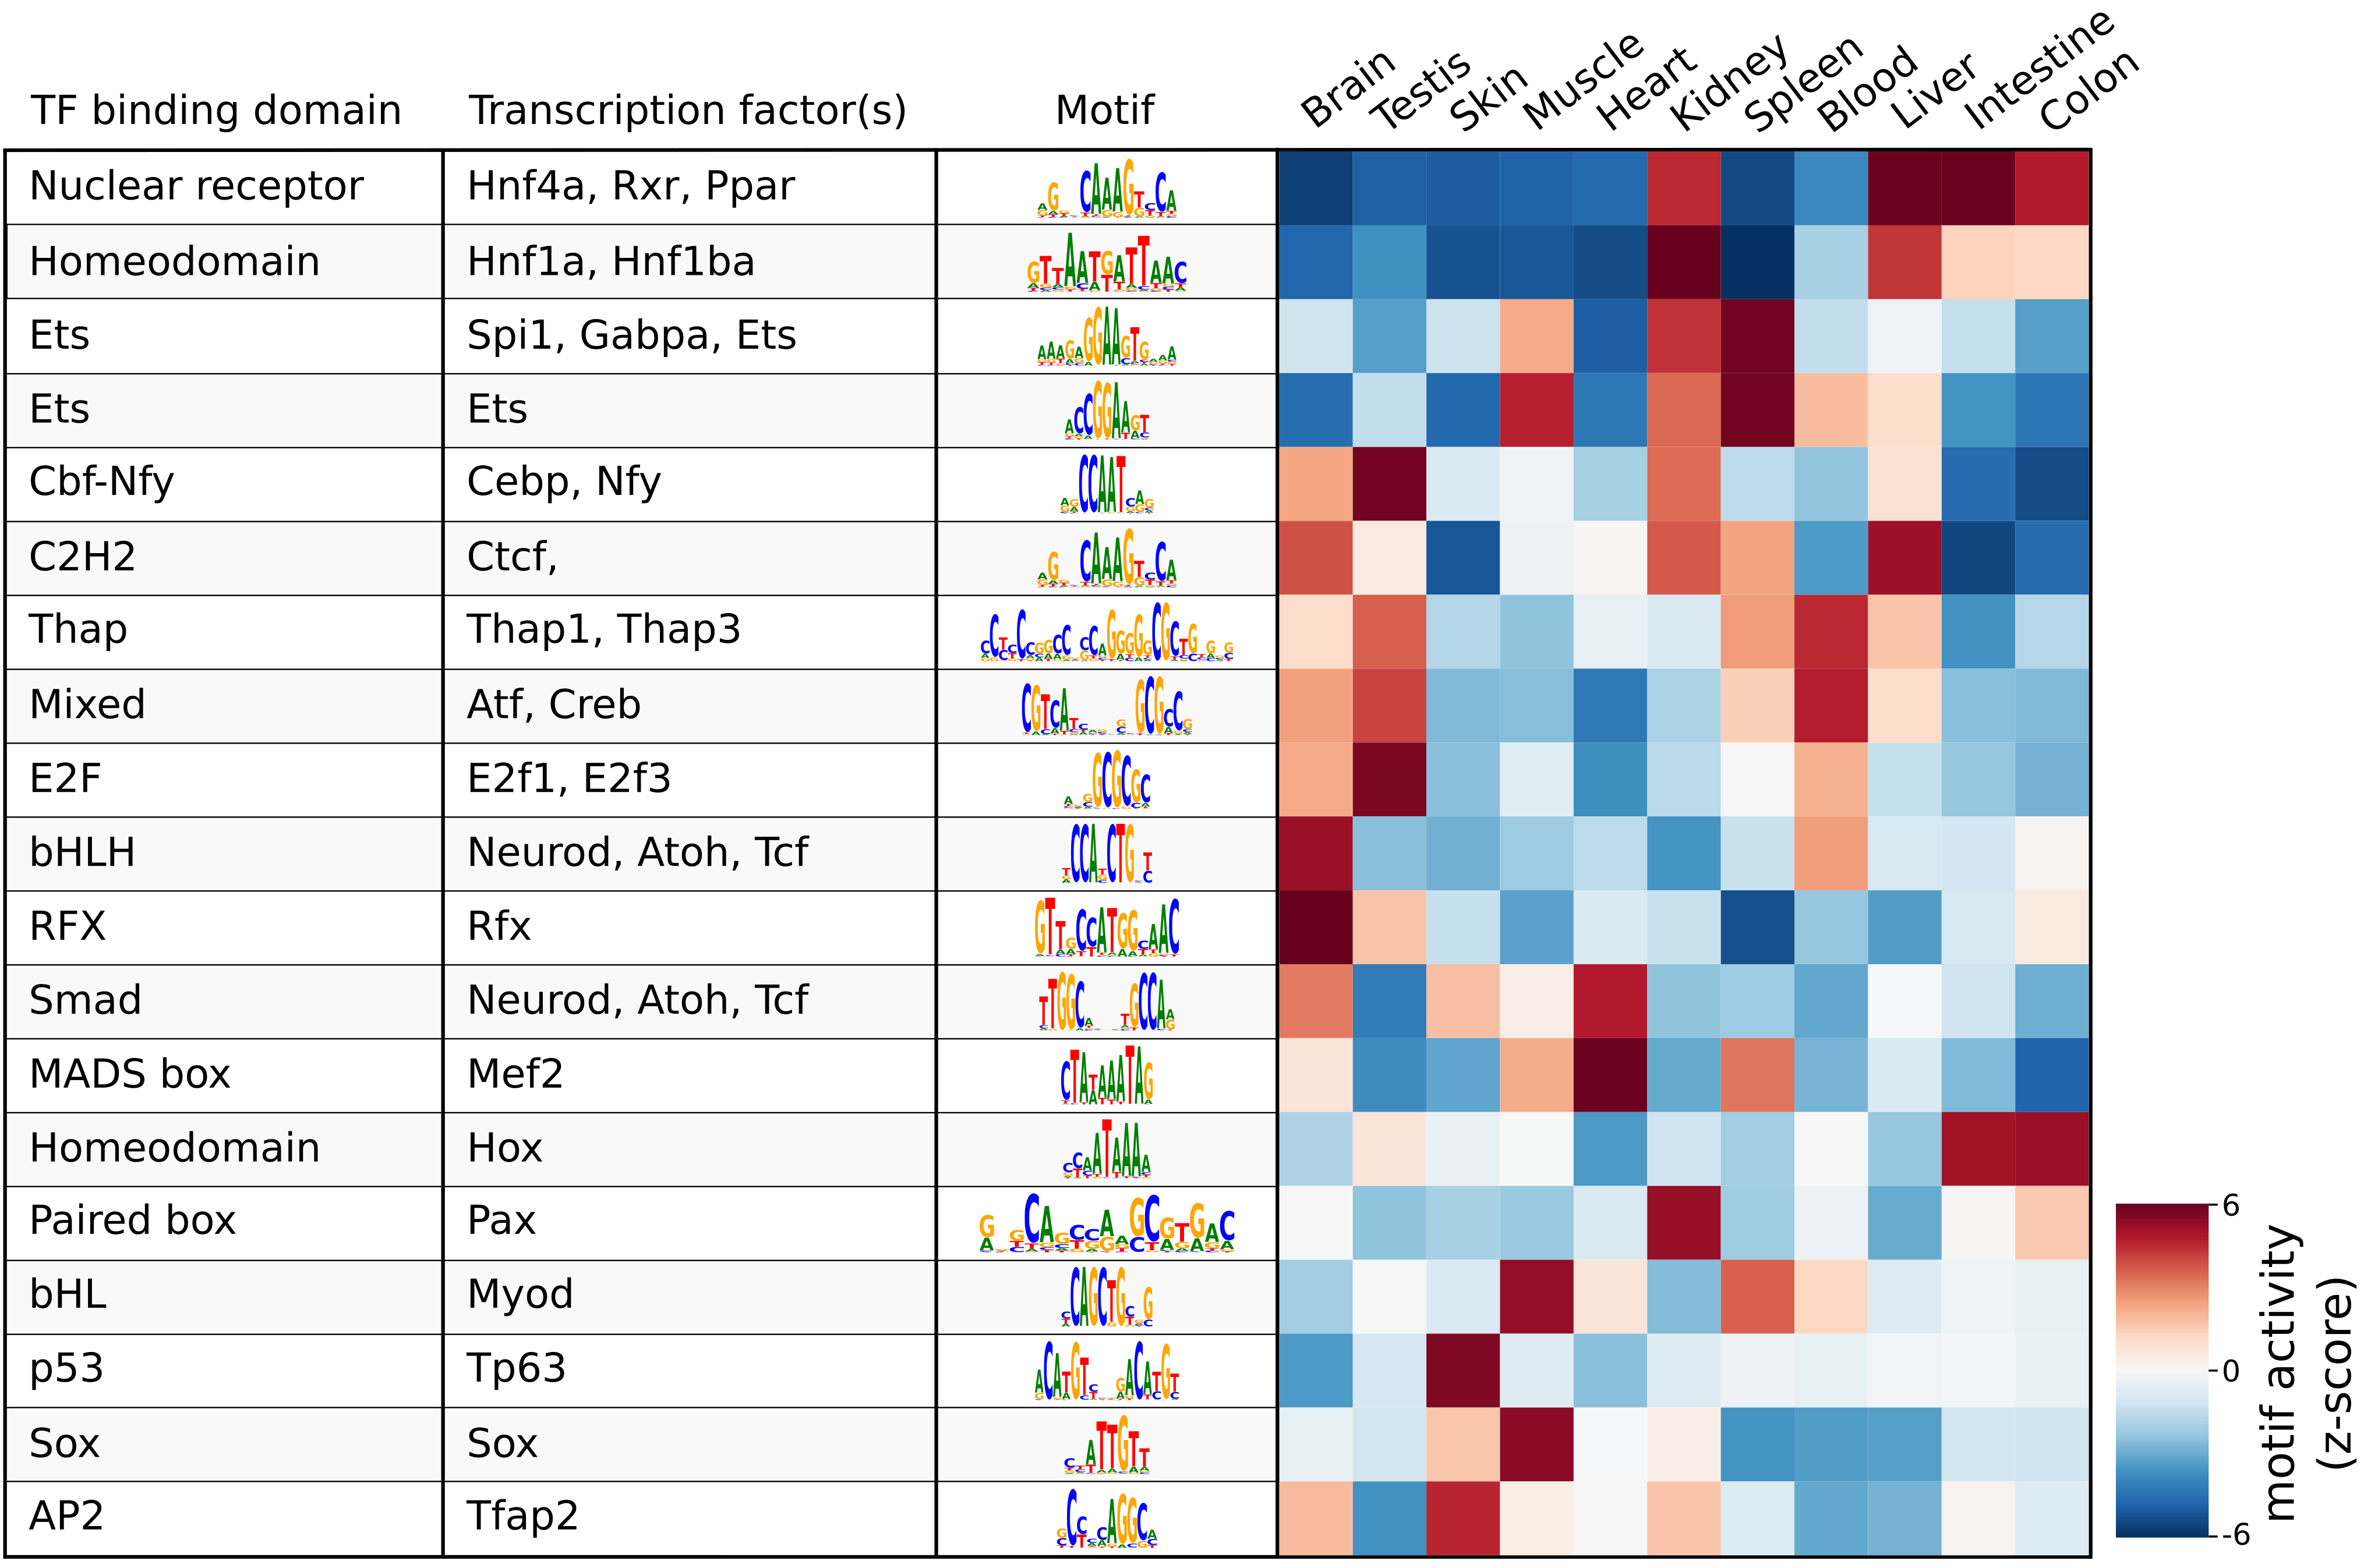
\includegraphics[width=\textwidth]{ch.seq2science/imgs/zebrafish_fig2.png}
	\caption{\label{fig:zebrafish_fig2} \textbf{Result of the differential motif analysis by seq2science between ATAC-seq peaks of different tissues of zebrafish} \cite{Yang2020}. Per tissue, the top two most differentially enriched motifs have been selected, with automatically inferred orthologs. The transcription factor names were manually curated for clarity. The full table with the motif analysis results is included in the quality report (Supplemental File S7).}
\end{figure}

In this example, we reproduced part of the analysis of the study "A map of cis-regulatory elements and 3D genome structures in zebrafish" \cite{Yang2020}. Yang et al. studied zebrafish chromosome conservation with a wide array of different functional genomics techniques. Here, we focused on the analysis of cis-regulatory elements and gene expression in different embryonic tissues. Using the default tools incorporated into seq2science, we downloaded the raw data for the different assays from the SRA, aligned these data to the zebrafish genome (\autoref{fig:zebrafish_fig1}A) and performed a differential transcription factor motif enrichment analysis on the ATAC-seq data. 

After running seq2science, we obtained a set of aligned BAM files, narrowPeak files, a count table, a trackhub, and a quality control report (see Supplemental Files S2-7 for the configuration, samples, and QC report). \autoref{fig:zebrafish_fig1}A shows the alignment of reads visualized using the UCSC trackhub that was created by seq2science. The figure shows histone modification ChIP-seq data (H3K4me3, H3K27ac, H3K9me2 and H3K9me3), ATAC-seq, and RNA-seq for three different tissues (brain, muscle and liver) on a region of chromosome 4. \autoref{fig:zebrafish_fig1}B-C show a selection of diagnostic plots from the quality report. \autoref{fig:zebrafish_fig1}B demonstrates the ratio of ATAC-seq peaks annotated to different genomic regions, created by ChIPseeker. \autoref{fig:zebrafish_fig1}C shows the correlation of reads in ATAC-seq peaks between samples. This figure illustrates the value of extensive quality control, as it shows two samples where the replicates do not cluster together (colon and intestine). This would warrant further investigation, as it could indicate a potential sample swap. In our experience, this occurs frequently with samples downloaded from public databases, which may be due to a sample swap in the original analysis, or during submission to the repository. 

As a demonstration of a more high-level analysis, \autoref{fig:zebrafish_fig2} shows the result of the differential motif analysis. Here, seq2science used GimmeMotifs to automatically convert the transcription factors in the motif database into the orthologous zebrafish genes. This automatic assignment means that motif analysis can also be used for non-model species that do not have a readily available motif annotation. \autoref{fig:zebrafish_fig2} shows the top motifs per tissue, based on the z-score. The complete table is part of the seq2science output report (see Supplemental File S7). In general, this unsupervised motif analysis recapitulates many of the findings of Yang et al., such as RFX and bHLH (Neurod, Atoh1) motifs enrichment in the brain and Hnf4a enrichment in the liver, colon, and intestine. Additionally, the GimmeMotifs analysis assigns Tp63 as a transcription factor enriched in the skin, as well as Tfap2, which are well-known regulators of epidermal development \cite{Soares2017,Li2019}.   

\subsection{The regulatory landscape of whole-body regeneration in the three-banded panther worm \textit{Hofstenia miasma}}

The article "Acoel genome reveals the regulatory landscape of whole-body regeneration" by Gehrke et al. analyzed the gene expression and chromatin accessibility of the Acoel worm \textit{Hofstenia miamia} \cite{Gehrke2019} during regeneration. The paper contains ATAC-seq and RNA-seq time-series data of the response to amputation and during whole-body regeneration. These data, and the \textit{Hofstenia miasma} genome are available from NCBI and consequently, seq2science can be applied to re-analyze this data with ease. The configuration files to reproduce the seq2science analysis and the complete output and quality control report are provided as Supplemental Information (Supplemental Files S8-13).

The seq2science ATAC-seq workflow generated a consensus peak set based on the union of peaks from all time points, together with a count table with the read quantification per time point. See Supplemental File S10 for the ATAC-seq QC report. We clustered the count table to visualize the temporal accessibility patterns using log-transformed and z-score normalized read counts (\autoref{fig:aah}A). The figure nicely recapitulates the original work, with most ATAC-seq peaks showing strong signal at either 0 hours or 48 hours post-amputation (hpa).

\begin{figure}
	\centering
	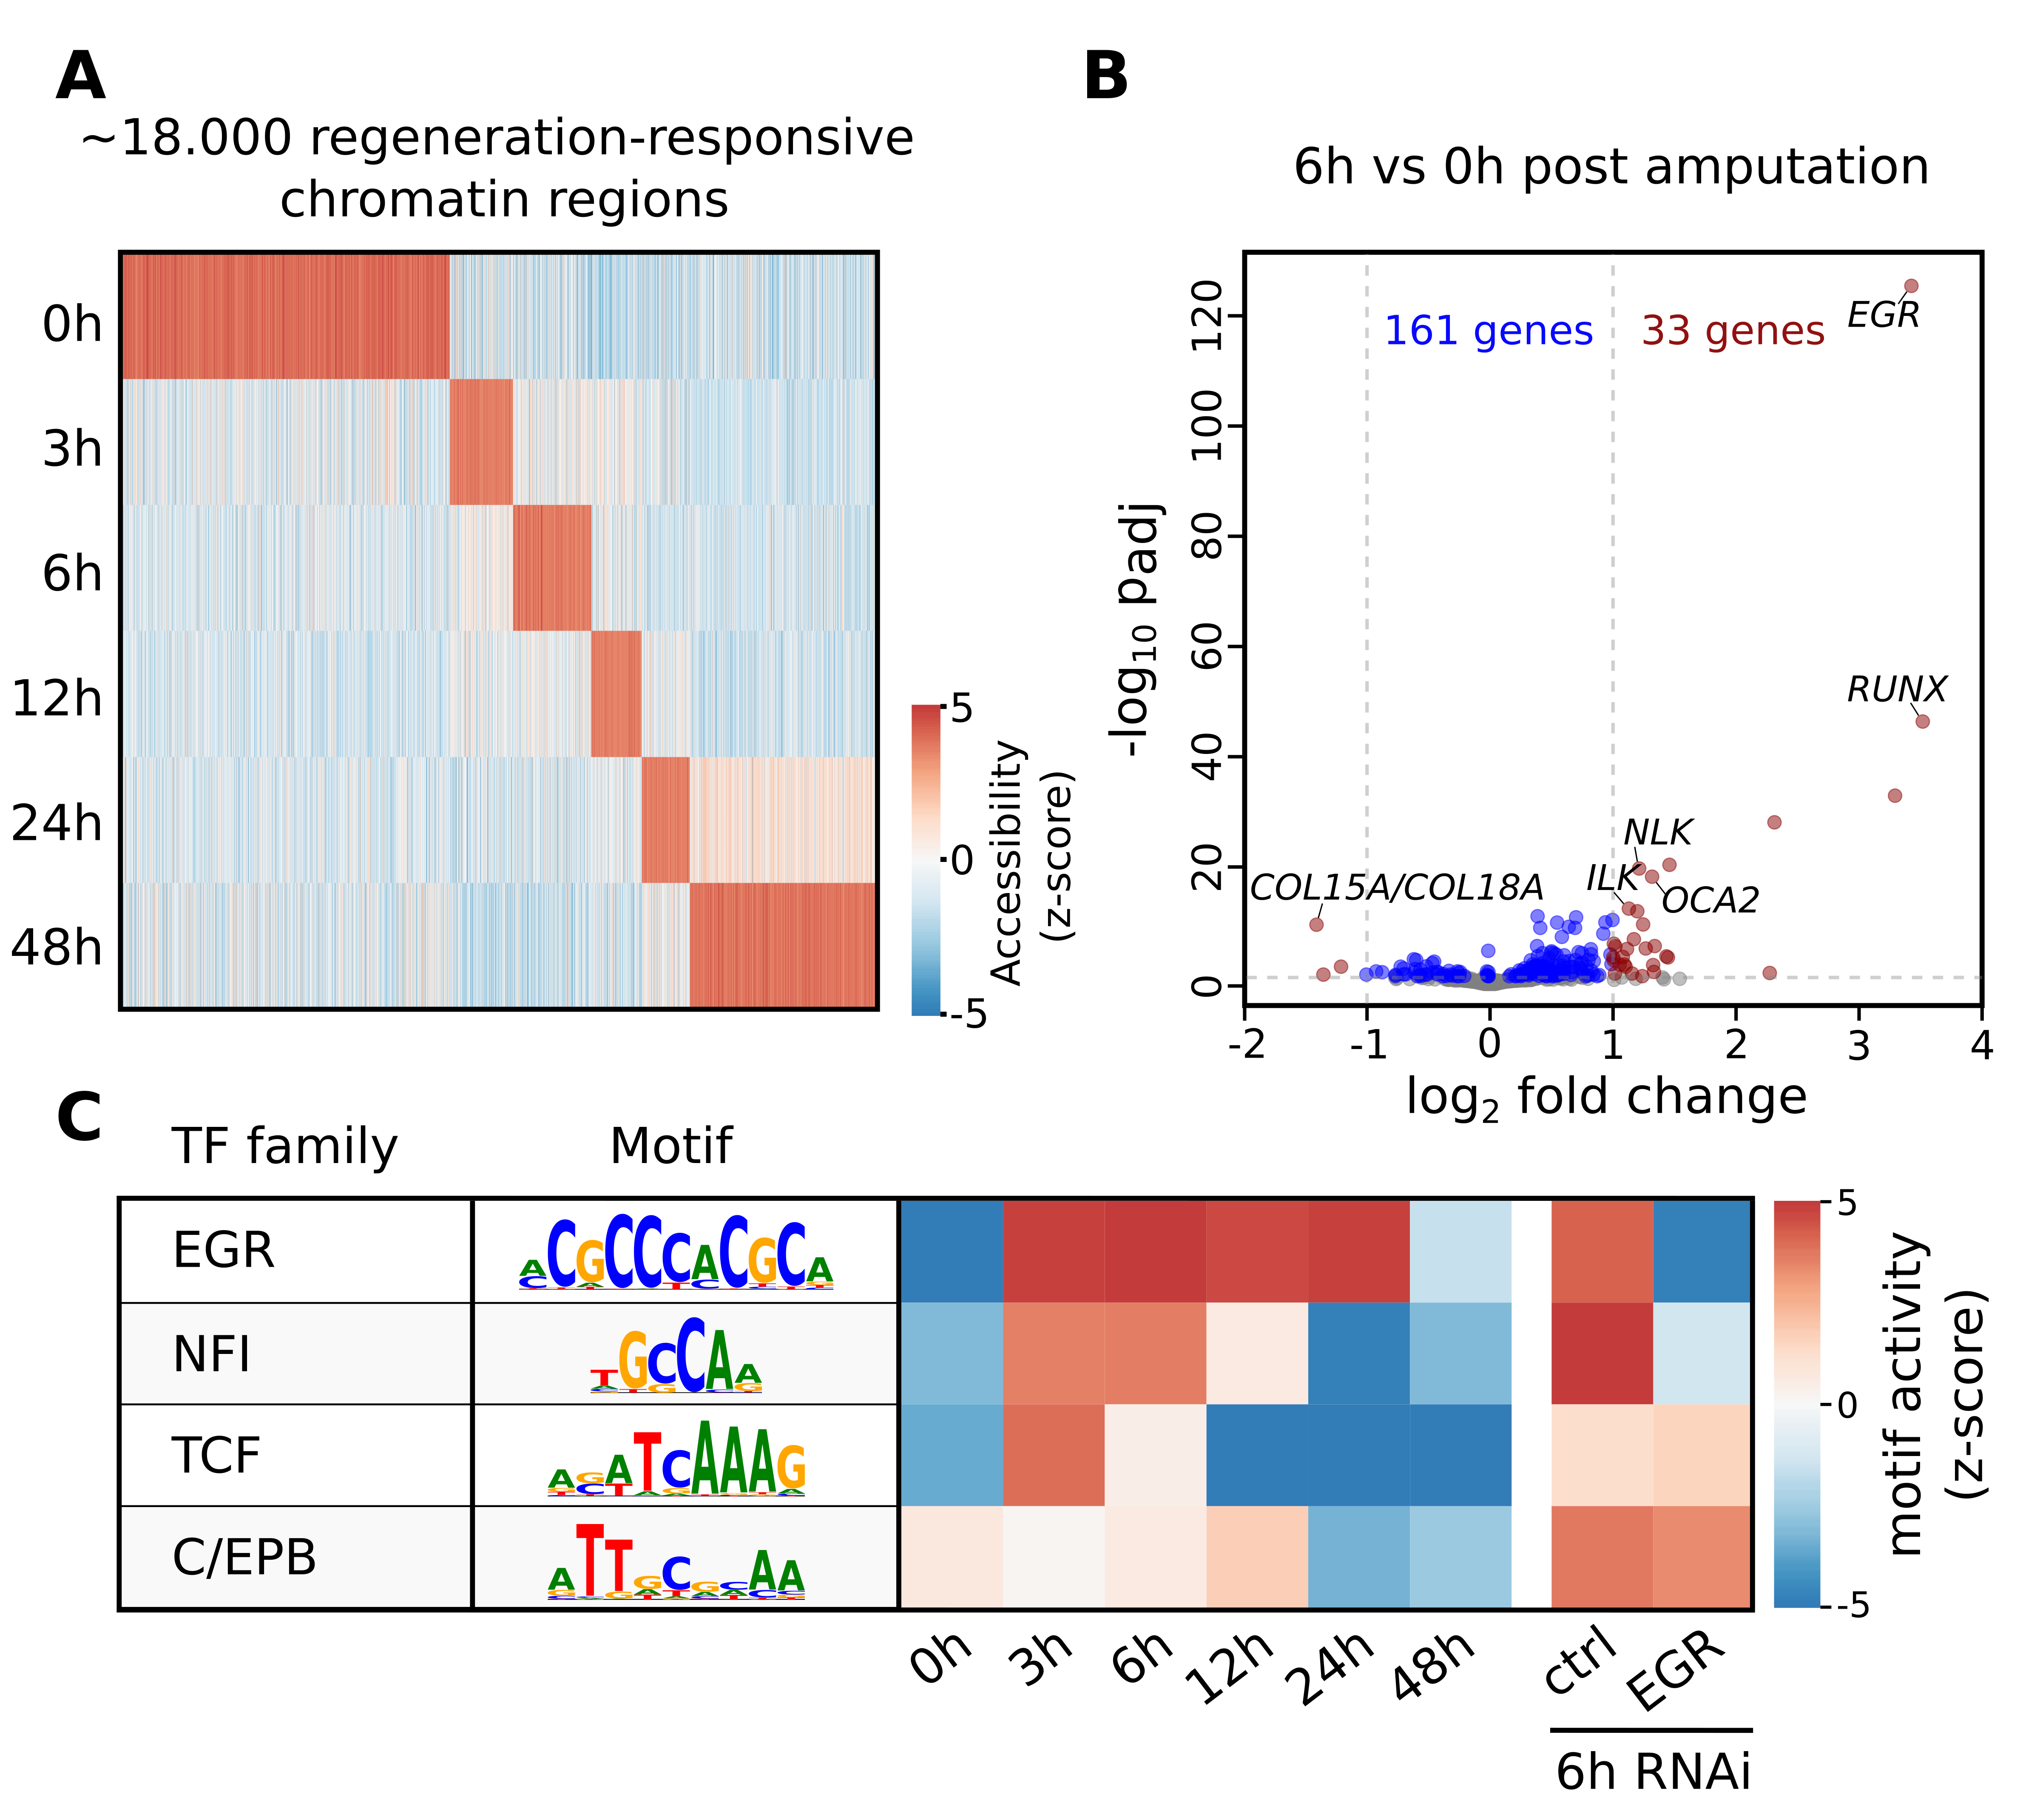
\includegraphics[width=0.8\textwidth]{ch.seq2science/imgs/figure_acoel.png}
	\caption{\label{fig:aah} \textbf{Summary of selected results from the re-analysis of the RNA-seq and ATAC-seq regeneration time series from Gehrke et al}. \textbf{(A)} Heatmap of \textit{Hofstenia miamia} chromatin accessibility during tail regeneration post amputation. ATAC-seq read counts provided by seq2science were log-transformed, and columns were normalized using the z-score. \textbf{(B)} Differential gene expression during tail regeneration. The X axis shows the log2 fold change of 6hpa vs 0hpa; the Y axis shows the -log10 transformed p-value. Significantly changed genes (padj $\leq$ 0.05; log2 fold change $\geq$ 1) are marked in red. Top results were labeled with human ortholog gene families. \textbf{(C)} Motif activity prediction during tail regeneration. The top four motifs, as identified by GimmeMotifs, are shown with the activity z-score predicted by gimme maelstrom. Both Gehrke et al. and our seq2science analysis identified the EGR and NFI motifs as the top differentially active motifs in the knockdown experiment.}
\end{figure}

To demonstrate the RNA-seq workflow, we performed a differential expression analysis of 6 hpa versus 0 hpa using DESeq2 (see  Supplemental File S13 for the complete output). The results are visualized as a volcano plot in \autoref{fig:aah}B. As reported, the \textit{Hofstenia miamia} EGR ortholog is the most significant differentially expressed gene, followed by the RUNX homolog \textit{runt}, which is involved in wound healing and regeneration. The role of \textit{egr} is further confirmed by the differential motif accessibility analysis, performed on the ATAC-seq peaks in the seq2science ATAC-seq workflow (\autoref{fig:aah}C). As stated earlier, GimmeMotifs automatically assigns the transcription factors in the database to the orthologous genes in our assembly. As expected, the top enriched motif is EGR, which shows a high z-score during the post-amputation time-series, from 3 to 24 hpa. After the knockdown of EGR using RNAi, this is the most depleted motif with a strong negative z-score. 

In conclusion, this use case reproduced the main findings from the the original paper, using the default tools incorporated in the RNA-seq and ATAC-seq workflows. Additionally, it demonstrates that seq2science is also easily applicable to non-model species.

\subsection{Map of human DNase I hypersensitive sites}

\begin{figure}
	\centering
	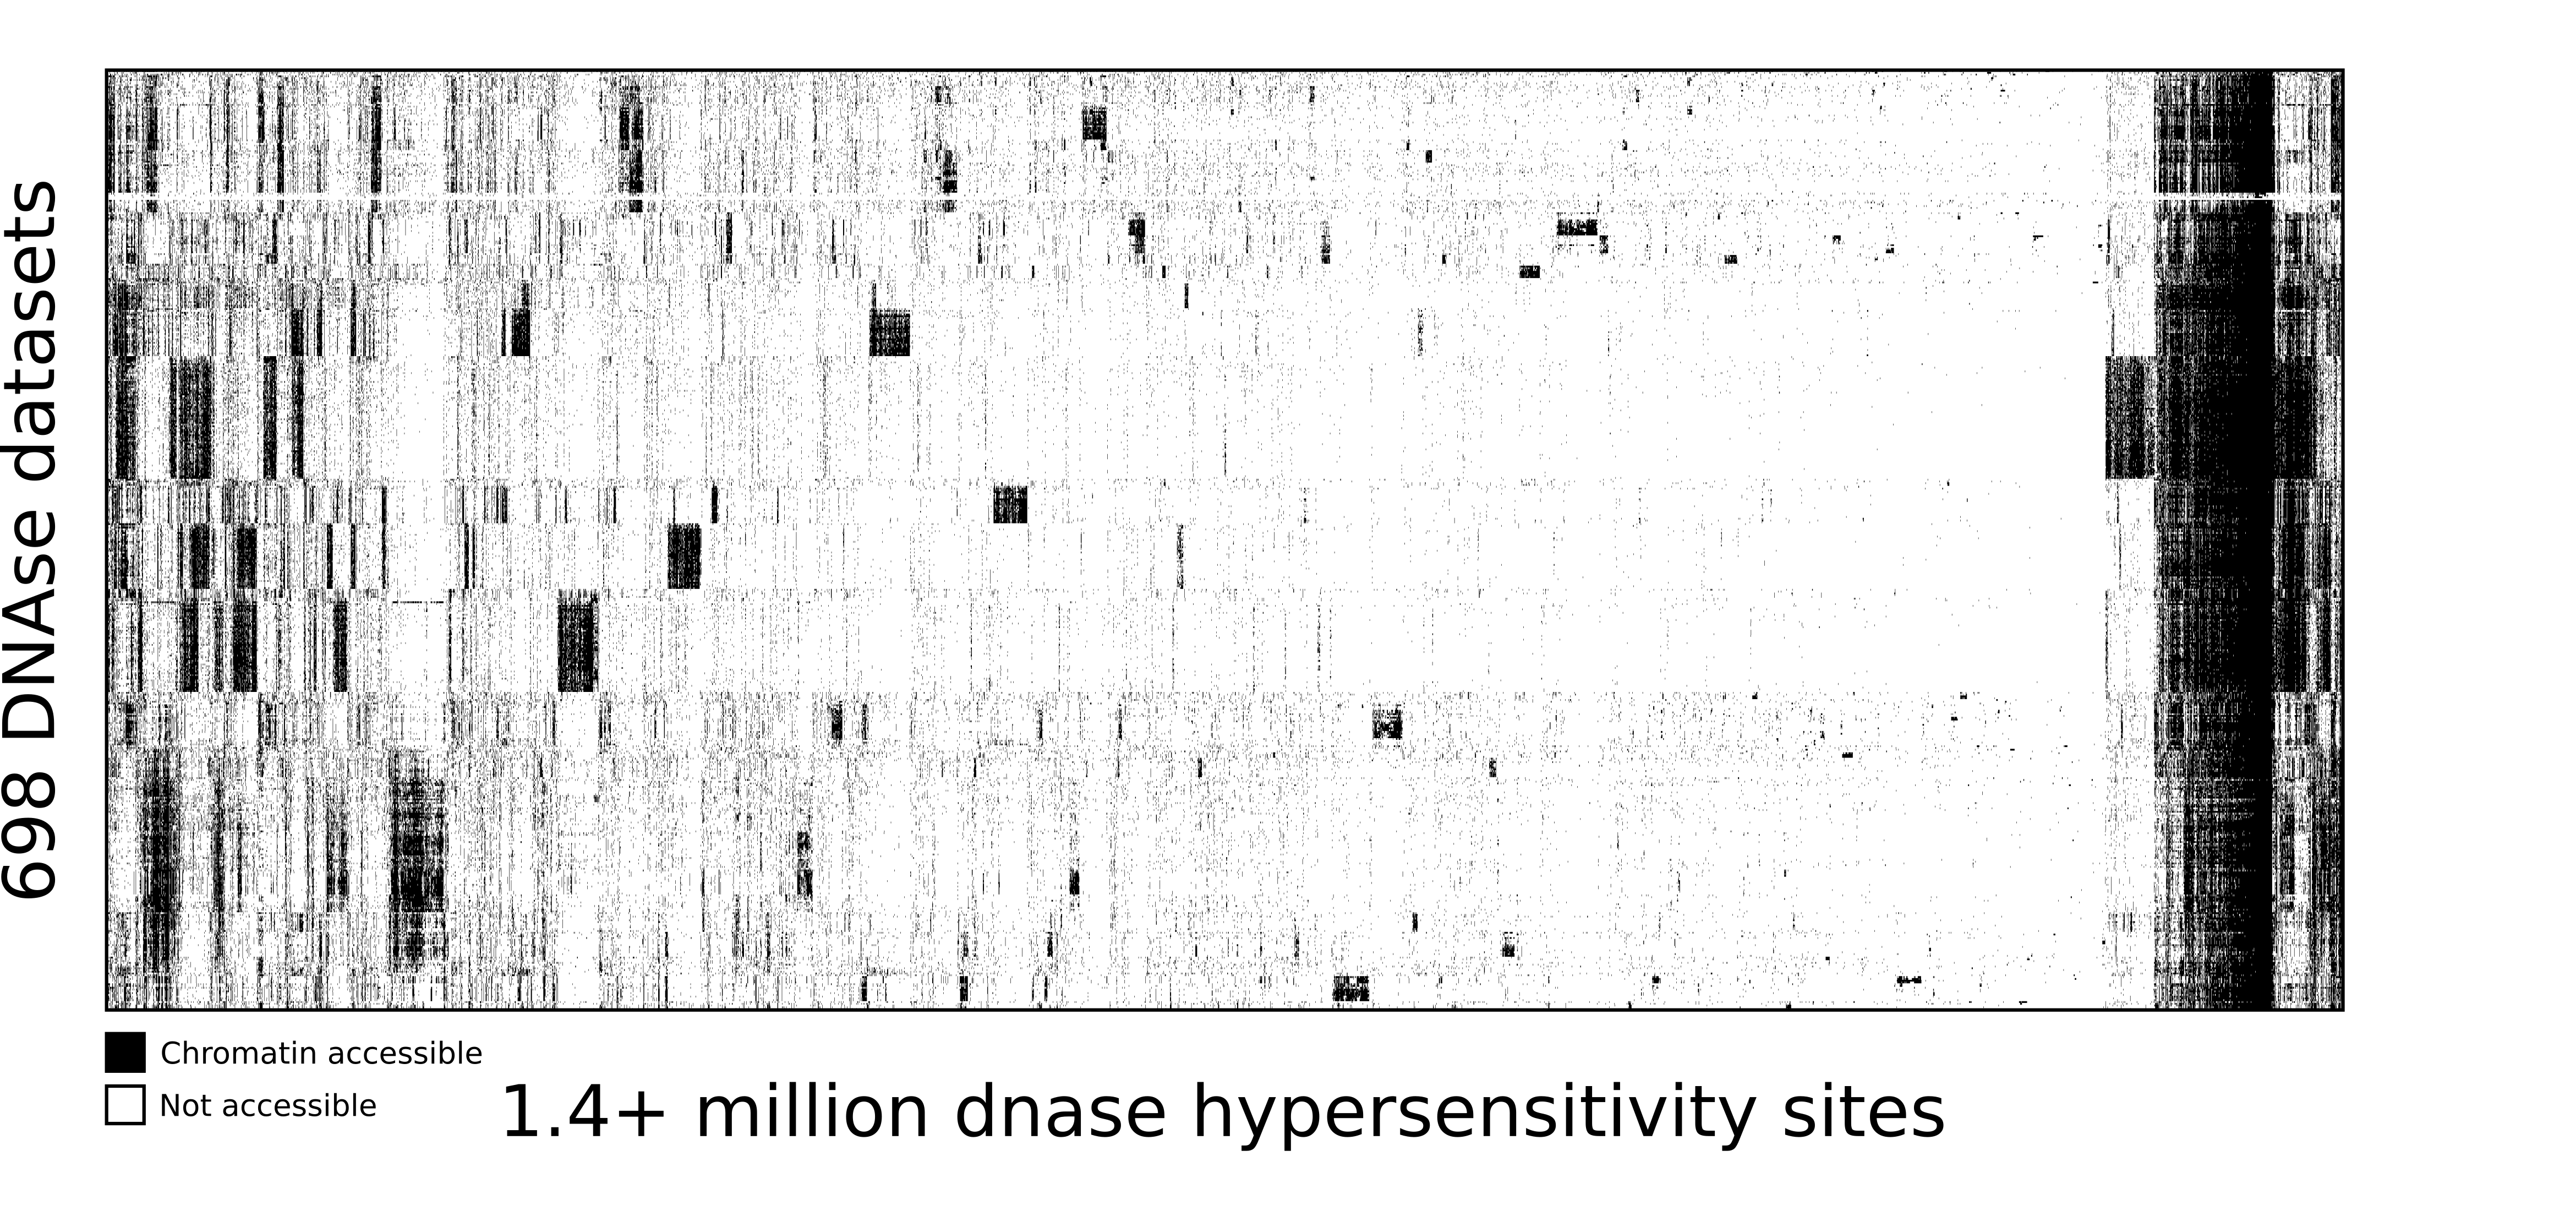
\includegraphics[width=0.9\textwidth]{ch.seq2science/imgs/dnase.png}
	\caption{\label{fig:dnase} \textbf{DNA accessibility at 1.4 million consensus DHSs assayed across 698 samples encapsulated in a visually compressed DHS-by-biosample matrix}. Recurring accessibility patterns indicate extensive sharing across cell contexts. Chromatin accessibility is defined as more than 1 count per million reads. }
\end{figure}

To highlight the ability of seq2science to scale with large data sets we performed a re-analysis of "Index and biological spectrum of human DNase I hypersensitive sites" \cite{Meuleman2020}. This paper analyzed 733 human DNAse I samples across different tissues. Of the 733 samples they reported, we were able to find 698 in the SRA database. To accommodate the DNAse I assay, which is not supported by default, we used the high degree of customizability of seq2science and adapted the default ATAC-seq workflow by turning the tn5\_shift flag off. The final output consists of over 1.7TB of sorted BAM files, with 1,404,721 peaks in the consensus peak set between these samples. \autoref{fig:dnase} shows the clustered output of the final count table, where the distinction between accessible and not accessible is made based on whether there is more than 1 count per million reads or not.

\section{Conclusion}

Seq2science facilitates reproducible preprocessing of high-throughput sequencing data of different assays through a unified setup. The tool is integrated with all major public sequence and assembly databases, and outputs extensive quality control and processed results to speed-up analysis. Seq2science requires minimal user input to get started, but offers a high degree of customizability. Each workflow and its configurable options are fully explained in the online documentation. The output from seq2science is reproducible and directly ready for analysis.

\section{Acknowledgements}

We are grateful to the open source bioinformatics community for their support in the development of seq2science. Special thanks to the bioconda and conda-forge teams for their help with packaging. More specifically we want to thank Saket Choudhary, Johannes K{\"o}ster, Tao Liu, Devon Ryan, and Phil Ewels for their assistance with Pysradb, Snakemake, MACS2, Bioconda, and MultiQC respectively. 

\chapter{Qnorm: fast-ish (and correct!) quantile normalization in Python}\thumbforchapter
\chaptermark{Qnorm}
\chapterauthor{Maarten van der Sande, Simon J. van Heeringen}
\newpage
\definecolor{bash_backcolor}{RGB}{48,10,36}

Quantile normalization made easy! This tool was developed as the current (Python) implementations scattered across the web do not correctly resolve collisions/ties in the ranks. Properly resolving rank ties is important when ties happen frequently, such as when working with discrete numbers (integers) in count tables. This implementation should be relatively fast, and can use multiple cores to sort the columns and tie-resolvement is accelerated by numba.

\section{Code example}

We recreate the example of Wikipedia\footnote{\url{https://en.wikipedia.org/wiki/Quantile_normalization}}:

\begin{lstlisting}[language=Python]
import pandas as pd
import qnorm

df = pd.DataFrame({'C1': {'A': 5, 'B': 2, 'C': 3, 'D': 4},
                   'C2': {'A': 4, 'B': 1, 'C': 4, 'D': 2},
                   'C3': {'A': 3, 'B': 4, 'C': 6, 'D': 8}})

print(qnorm.quantile_normalize(df, axis=1))

         C1        C2        C3
A  5.666667  5.166667  2.000000
B  2.000000  2.000000  3.000000
C  3.000000  5.166667  4.666667
D  4.666667  3.000000  5.666667
\end{lstlisting}

It is important to note that qnorm standardizes along columns by default, like in the wiki example above. However \lstinline[language=Python]{qnorm.quantile_normalize} accepts an (optional) axis argument, which can be used to change this behaviour. If \lstinline[language=Python]{axis=1} (default), standardize along columns, if \lstinline[language=Python]{axis=0`}, standardize along rows.

\begin{itemize}
    \item note: pandas is an optional dependency of qnorm, and if you want to quantile normalize dataframes make sure to install pandas yourself (conda/pip install pandas).

    \item note: you can also pass numpy arrays as input to \lstinline[language=Python]{qnorm.quantile_normalize}.
\end{itemize}

\section{Multicore support}

To accelerate the computation you can pass a ncpus argument to the function call and qnorm will be run in parallel:

\begin{lstlisting}[language=Python]
qnorm.quantile_normalize(df, ncpus=8)  
\end{lstlisting}

\section{Normalize onto distribution}

You can also use the \lstinline[language=Python]{qnorm.quantile_normalize} function to normalize "onto" a distribution, by passing a target along to the function call.

\begin{lstlisting}[language=Python]
import pandas as pd
import qnorm

df = pd.DataFrame({'C1': {'A': 4, 'B': 3, 'C': 2, 'D': 1},
                   'C2': {'A': 1, 'B': 2, 'C': 3, 'D': 4}})

print(qnorm.quantile_normalize(df, target=[8, 9, 10, 11]))

     C1    C2
A  11.0   8.0
B  10.0   9.0
C   9.0  10.0
D   8.0  11.0
\end{lstlisting}

\section{How fast is it and what is its memory usage?}

How better to measure this than a little benchmark/example? For this example, we will consider 100 replicates, each consisting of one million integer values between 0 and 100, which should give us plenty of rank ties.

\begin{lstlisting}[language=Python]
import numpy as np
import qnorm

test = np.random.randint(0, 100, size=(1_000_000, 100), dtype=np.int32)

qnorm.quantile_normalize(test, ncpus=4)
\end{lstlisting}

Of which we can now check how long it takes with a little bash script:

\begin{mdframed}[
    backgroundcolor=bash_backcolor,
    hidealllines=true,
    innertopmargin=0pt,
    innerbottommargin=0pt,
    innerleftmargin=0pt,
    innerrightmargin=0pt
]
\begin{lstlisting}[escapechar=\%,language=bash,basicstyle=\ttfamily\color{white}]
user@comp:%$\mathtt{\sim}$%$ /usr/bin/time --verbose python small_qnorm_script.py \
|& grep -P "(wall clock|Maximum resident set size)"

Elapsed (wall clock) time (h:mm:ss or m:ss): 0:07.52
Maximum resident set size (kbytes): 2768884
\end{lstlisting}
\end{mdframed}

It takes only 7.5 seconds to initialize our table and quantile normalize it. I think that's pretty fast!

The test array we made consists of 100 * 1.000.000 = 100.000.000 single point precision integers, so four bytes each (400.000.000 bytes, 0.4 gigabytes). The memory footprint of our script is 0.27 gigabytes, around 7 times our input. Unfortunately that makes qnorm a bit memory hungry, but that should not be a problem in 99\% of the cases. If memory usage is a problem take a look at the supported low-memory implementation.

\subsection{Scaling of ncpus}

Using more than four cpus generally does not lead to a much bigger speedup.

\begin{figure}[H]
	\centering
	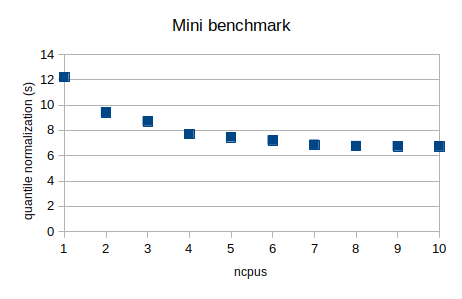
\includegraphics[width=0.5\textwidth]{ch.qnorm/imgs/benchmark_cores.png}
	\caption{\label{fig:benchmark_cores}\textbf{Qnorm wall clock time for different number of cores.}}
\end{figure}

\subsection{Incremental quantile norm}

In case you want to quantile normalize excessively large tables, there is a ``memory-efficient'' implementation. This implementation gets its memory efficiency by calculating the mean ``online'', which means we calculate it on fractions of the total table and then update the value. The other change is that intermediate results are written to disk. This means that this implementation effectively swaps memory to disk, and thus is not ``memory hungry'', but instead ``disk hungry''. This incremental method however can scale to virtually infinitely large tables (or until you run out of disk space).

Let's say we want to do something crazy like quantile normalize the human genome in 10 basepair bins. That means we will have around 300.000.000 values per sample. File-based qnorm works with both csv/tsv, parquet, and hdf files. For this example, we will work with hdf files (make sure to set \lstinline[language=Python]{data_columns=True}). Parquet and hdf files also are fast, but csv/tsv files are (very) slow because of the enormous amount of I/O they require.

\begin{lstlisting}[language=Python]
df = pd.DataFrame(
    index=range(300_000_000), 
    dtype=int, 
    columns=['sample'+str(col) for col in range(64)]
)
df[:] = np.random.randint(0, 100, size=df.shape)
df.to_hdf('hg_bins.hdf', key='qnorm', format='table', data_columns=True)
\end{lstlisting}

We can now compare the speed and memory of the file-based method vs the "standard" method.

\begin{lstlisting}[language=Python]
import qnorm

# incremental qnorm (reads hg_bins.hdf from disk and writes
# output to hg_bins_qnorm.hdf) 
qnorm.incremental_quantile_normalize(
    'hg_bins.hdf', 
    'hg_bins_qnorm.hdf', 
    rowchunksize=500_000, 
    colchunksize=4, 
    ncpus=4
)

# standard
df = pd.read_hdf(f'hg_bins.hdf').astype('float32')
df_qnorm = qnorm.quantile_normalize(df, ncpus=4)
\end{lstlisting}

\begin{figure}[H]
	\centering
	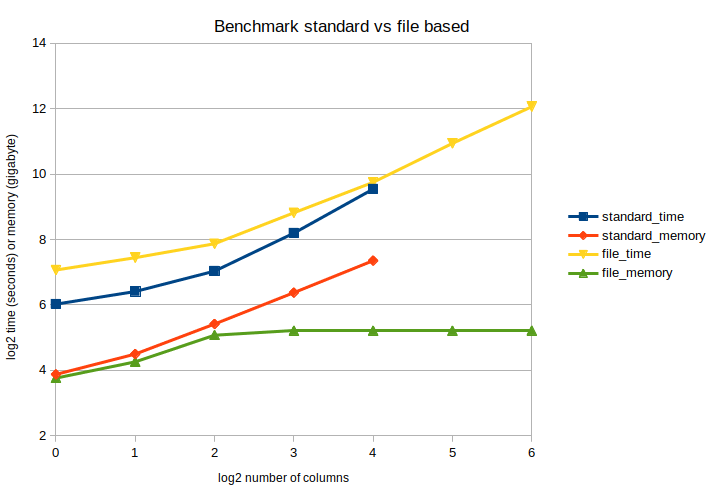
\includegraphics[width=0.5\textwidth]{ch.qnorm/imgs/benchmark_file.png}
	\caption{\label{fig:benchmark_file}\textbf{Qnorm wall clock time and memory usage for standard and file-based quantile normalization.} The benchmark was run on a dataset with 300.000.000 rows.}
\end{figure}

The standard method does not come farther than $2^4=16$ samples before running out of memory on a 512-gigabyte system! The incremental method has similar timings and even seems to scale better than the standard method for large arrays. And it takes only an hour to normalize 64 samples.

The rowchunksize and colchunksize respectively influence how large of chunks the output is written to disk and how many columns are being sorted and quantile normalized at the same time. Generally speaking, the larger the better, however, the defaults should most of the time be sufficiently fast.

\begin{itemize}
    \item note: Both in-memory normalization and incremental normalization should produce identical results, and neither is more correct than the other.

    \item note: note: The incremental implementation requires pandas to be installed (conda/pip install pandas).

    \item note: When using hdf files make sure to install (py)tables (conda install pytables or pip install tables).

    \item note: When using parquet files make sure to install pyarrow (conda install pyarrow or pip install pyarrow).

    \item note: The input format specifies the output format.

    \item note: Because of the design of hdf5, there is a limit on the number of columns it can hold. In case you have a lot of columns (500+), it is probably best to use parquet and not hdf5.

\end{itemize}

\section{Command Line Interface (CLI) example}

Qnorm also contains a CLI for converting csv/tsv files. The CLI depends on pandas, but this is an optional dependency of qnorm. To make use of the CLI make sure to install pandas in your current environment as well!

\begin{mdframed}[
    backgroundcolor=bash_backcolor,
    hidealllines=true,
    innertopmargin=0pt,
    innerbottommargin=0pt,
    innerleftmargin=0pt,
    innerrightmargin=0pt
]
\begin{lstlisting}[escapechar=\%,language=bash,basicstyle=\ttfamily\linespread{1.15}\footnotesize\color{white}]
user@comp:%$\mathtt{\sim}$%$ qnorm --help

usage: qnorm [-h] [-v] table

Quantile normalize your table

positional arguments:
  table          input csv/tsv file which will be quantile normalized

optional arguments:
  -h, --help     show this help message and exit
  -v, --version  show program's version number and exit
\end{lstlisting}
\end{mdframed}

And again the example of Wikipedia:

\begin{mdframed}[
    backgroundcolor=bash_backcolor,
    hidealllines=true,
    innertopmargin=0pt,
    innerbottommargin=0pt,
    innerleftmargin=0pt,
    innerrightmargin=0pt
]
\begin{lstlisting}[escapechar=\%,language=bash,basicstyle=\ttfamily\linespread{1.15}\footnotesize\color{white}]
user@comp:%$\mathtt{\sim}$%$ cat table.tsv
        C1      C2      C3
A       5       4       3
B       2       1       4
C       3       4       6
D       4       2       8

user@comp:%$\mathtt{\sim}$%$ qnorm table.tsv
        C1                C2                C3
A       5.66666666666     5.16666666666     2.0
B       2.0               2.0               3.0
C       3.0               5.16666666666     4.66666666666
D       4.66666666666     3.0               5.66666666666
\end{lstlisting}
\end{mdframed}

\begin{itemize}
    \item note: the qnorm cli assumes that the first column and the first row are used as descriptors, and are "ignored" in the quantile normalization process. Lines starting with a hashtag "\#" are treated as comments and ignored.

    \item note: The CLI requires pandas to be installed (conda/pip install pandas)
\end{itemize}

\section{Installation}

\subsection{pip}

\begin{lstlisting}[escapechar=\%,language=bash,basicstyle=\ttfamily\color{white}]
user@comp:%$\mathtt{\sim}$%$ pip install qnorm
\end{lstlisting}

\subsection{conda}

Installing qnorm from the conda-forge channel can be achieved by adding conda-forge to your channels with:

\begin{lstlisting}[escapechar=\%,language=bash,basicstyle=\ttfamily\color{white}]
user@comp:%$\mathtt{\sim}$%$ conda config --add channels conda-forge
\end{lstlisting}

Once the conda-forge channel has been enabled, qnorm can be installed with:

\begin{lstlisting}[escapechar=\%,language=bash,basicstyle=\ttfamily\color{white}]
user@comp:%$\mathtt{\sim}$%$ conda install qnorm
\end{lstlisting}

\subsection{local}

clone the repository

\begin{lstlisting}[escapechar=\%,language=bash,basicstyle=\ttfamily\color{white}]
user@comp:%$\mathtt{\sim}$%$ git clone https://github.com/Maarten-vd-Sande/qnorm
\end{lstlisting}

And install it

\begin{mdframed}[
    backgroundcolor=bash_backcolor,
    hidealllines=true,
    innertopmargin=0pt,
    innerbottommargin=0pt,
    innerleftmargin=0pt,
    innerrightmargin=0pt
]
\begin{lstlisting}[language=bash,basicstyle=\ttfamily\color{white}]
user@comp:%$\mathtt{\sim}$%$ cd qnorm
user@comp:%$\mathtt{\sim}$%$ pip install .
\end{lstlisting}
\end{mdframed}

% \chapter{The phylotypic stage is undefined; crucial controls missing for comparative studies}\thumbforchapter
\chaptermark{The phylotypic stage is undefined}
\chapterauthor{Maarten van der Sande, Marlien Kolmus, Gert Jan C. Veenstra, Simon J. van Heeringen}
\newpage

\section{Abstract}

The phylotypic stage is the stage with the highest degree of similarity during embryonic development between species of the same phylum. Similarity used to be defined as morphological similarity, but more recently has been defined as molecular similarity and in turn analyzed as such. The phylotypic stage is, however, a poorly defined concept with no clearly defined expectations. It is undefined whether the same point of maximum similarity exists for comparisons within the same species or for comparisons between phyla. This lack of a clear definition complicates the analysis of the phylotypic stage. We re-analyzed four comparative molecular studies of the phylotypic stage and identify issues with their experimental design and in turn interpretation of their results. To help identify these issues we propose that studies about the phylotypic stage at least include a within-species, a within-phylum, and a between-phylum comparison. Additionally, we advocate for a re-definition of the phylotypic stage, as it is ambiguous in its current form.

\section{Introduction}

Embryonic development is a complex and highly orchestrated process that begins with a single fertilized egg and culminates in the formation of a multicellular organism with a defined body plan and specialized organs. Even though morphologically the eggs and adults can be vastly different between two related species, a remarkable period of similarity occurs in early development. This period of similarity is known as the phylotypic stage, and over the years many different theories and explanations for its existence have been proposed\cite{Kalinka2012,Irie2014,Drost2017}.  

The idea of a morphologically similar embryonic stage between species dates back to Aristotle\cite{Aristotle1943} but was formalized and popularized by Karl Ernst von Baer and Ernst Haeckel\cite{haeckel1866,baer1828}. In the early 1800s, von Baer formulated his four laws of embryology based on post-gastrulation embryos. His first law states that \textit{the more general characters of a large group appear earlier in the embryo than the more special characters}. This means that as an embryo develops, it first develops its oldest phylum-specific features, to then respectively develop its class, order, family and species-specific features. Haeckel instead formulated the recapitulation theory, popularized by the phrase \textit{ontogeny recapitulates phylogeny}. The recapitulation theory states that an embryo consecutively develops from embryonic stages of ancestral species to stages of descendants. In its strongest form, the recapitulation theory has been discredited, as development is not a repetition of evolution\cite{ehrlich1974}. Nonetheless, Haeckel's observations of similarities between embryos of different vertebrate classes, have, together with von Baers’ laws, formed the basis for the current models of evolutionary development

The notion of similar embryonic development between species has led to two competing models of evolutionary development, the hourglass model and the funnel model (also known as the early-conservation model). The hourglass model is based on the model proposed in 1954 by Paul Medawar\cite{Medawar1954}. Medawar argues that somewhere mid-embryogenesis is the most morphologically conserved stage for vertebrates. This has since been generalized across phyla and even kingdoms (plants\cite{Quint2012} and fungi\cite{Cheng2015}), where each phylum now has its own stage of maximum similarity during mid-embryogenesis. The funnel model, based on von Baers' laws, instead predicts the highest morphological similarity early in development. The phylotypic stage, initially called the \textit{phyletic stage}, refers to the point of maximum similarity in these models\cite{Cohen1963, Seidel1960}. More recently an inverse hourglass model has been proposed for comparisons between phyla, where specifically the beginning and end of embryonic development seem conserved, and the least molecular similarity is seen at the phylotypic stage\cite{Levin2016}.

Whereas the phylotypic stage has originally been defined based purely on morphological descriptions alone, the definition is gradually being extended to contain molecular features. For example, the popular idea that HOX genes are master regulators of the phylotypic stage for vertebrate development\cite{Duboule1994}. More recently genome-wide comparisons of genes and regulatory elements have been applied. These quantitative comparisons can roughly be divided into two distinct approaches; (i) calculating a conservation metric for a single time series for each time point, where conservation metrics include for instance the average evolutionary age of transcripts\cite{DomazetLoso2010}, gene mutation rate index\cite{Quint2012, Piasecka2013}, embryonic lethality\cite{Uchida2018}, relation between timing of DNA accessibility and its evolutionary age\cite{Uesaka2019}, and variance between replicates\cite{Liu2020, Uchida2022}. These results are usually visualized as a figure where one axis represents embryonic development, and the other the calculated conservation metric. The second approach (ii) compares orthologous features between time points of two time-series directly. Orthologous features that have been compared are cell type proportions\cite{Mayshar2023}, gene expression similarity\cite{Irie2011, Kalinka2010, Levin2016, marletaz2018}, and regulatory DNA accessibility similarity\cite{Hu2017, Liu2021}. The comparison between two time-series is usually visualized as a heat map, where the axes represent embryonic development per species, and the color represents (dis)similarity (see figure \ref{fig:models}). Both of these quantitative approaches have been used to study the phylotypic stage, but there are subtle differences in the conclusions one can draw depending on which method is used. 

\begin{figure}[H]
    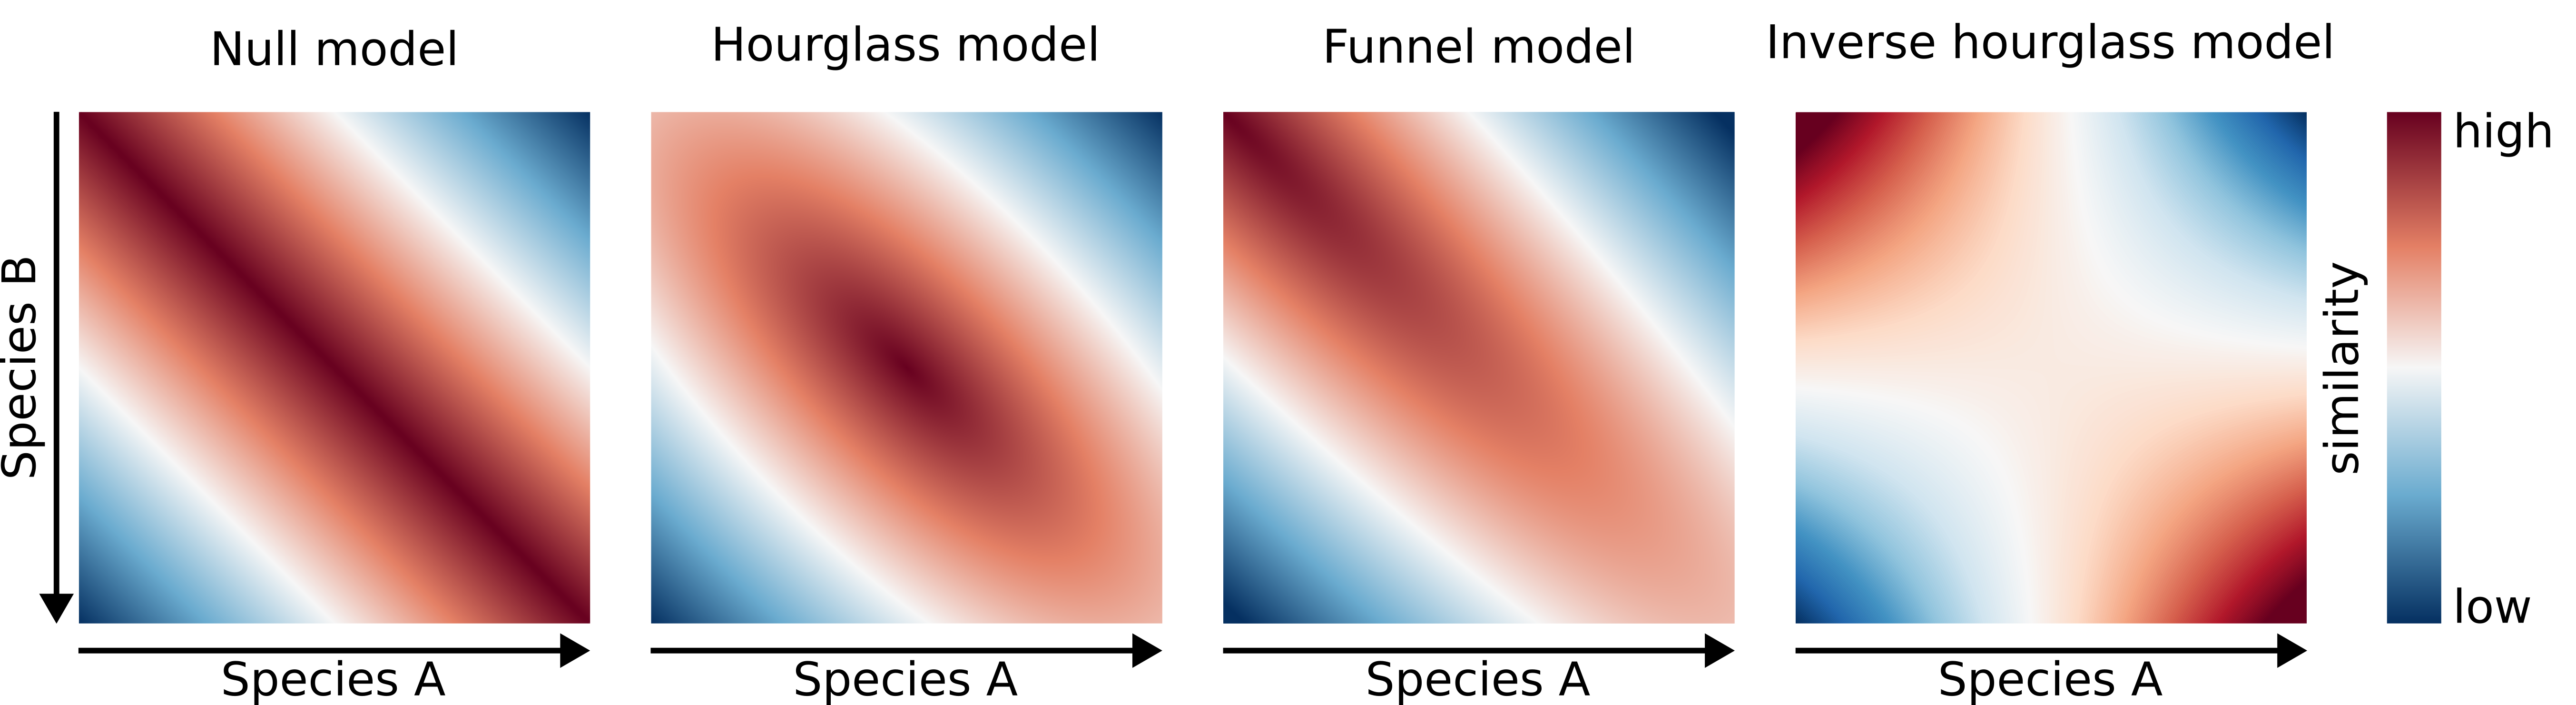
\includegraphics[width=\linewidth]{ch.hourglass/images/models.png}
    \caption{\textbf{Schematic representation of developmental similarity along embryonic development for different comparative models}. These figures are usually read ordered from top-left to bottom-right, where the x-axis represents embryonic development for species A, and the y-axis represents embryonic development for species B. The null model represents the case where there are no developmental stages of higher or lower similarity between two species. The hourglass model predicts a point of maximum similarity somewhere mid-embryogenesis for species of the same phylum, and the funnel model instead predicts the highest similarity at the start of embryonic development. The inverse hourglass model predicts that for comparisons between phyla that there is a point mid-development that is least conserved.}
    \label{fig:models}
\end{figure}

While quantitative studies are seen as offering an unbiased approach to studying the phylotypic stage, the results can be heavily influenced by experimental design, which highlights the importance of incorporating appropriate controls. To give some examples; based on morphological timings both an hourglass\cite{Cordero2020} and a within-phylum inverse hourglass\cite{OlafRP2003} have been found. Based on RNA-seq data Chan \textit{et al.} found an hourglass pattern, but with the same analysis on microarray data they find no temporal conservation pattern\cite{Chan2021}. Piasecka \textit{et al.} find that the observed conservational pattern is highly dependent on the metric used, for instance that the protein sequence of regulatory regions is most conserved for genes expressed in mid-development, gene duplication and new gene introduction is most constrained during early development, but all gene properties coherently show the least conservation for the latest stages\cite{Piasecka2013}. Moreover, a popular similarity metric, the transcriptomic age index\cite{DomazetLoso2010}, expresses completely different conservational patterns based on whether or not the data has been log transformed\cite{Piasecka2013}. Finally, Levin \textit{et al.} found an inverse hourglass between members of different phyla\cite{Levin2016}, but in an independent re-analysis this pattern was found not to be significantly enriched\cite{Dunn2018}. 

To address the issue of the dependence on experimental design when studying the phylotypic stage we propose three crucial controls when studying the phylotypic stage; (i) a within-phylum comparison, (ii) a between-phylum comparison, and (iii) a within-species comparison. No study about the phylotypic stage to date incorporates all three controls, and we show that by applying these comparisons to earlier analyses we find problematic statistical artefacts which lead to incorrect conclusions about the phylotypic stage. Moreover, by specifically addressing these controls the field can work towards a unified definition of the phylotypic stage and its related models.

\section{What does the phylotypic stage actually predict?}

To have a constructive discussion about the phylotypic stage it is crucial to explicitly define it. An explicit definition gives clarity, identifies assumptions and hypotheses, but most importantly is falsifiable. Currently, the phylotypic stage lacks a universally accepted definition, and the different definitions are far from explicit. The current definitions can roughly be divided into three main ideas; the presence of a dynamic pattern, the complexity of gene regulation at the phylotypic stage, or the presence of certain key morphological characteristics\cite{OlafRP2003}. The dynamic pattern-based definition describes the pattern of similarity, where similarity can both be morphological or molecular\cite{Slack1993,Duboule1994}. The pattern-based definition predicts the highest similarity at the phylotypic stage. The gene-regulatory based definition specifically predicts that gene regulation during the phylotypic stage is so complex that small changes in gene expression result in large (deadly) effects \cite{raff1996}. Finally, the key morphological characteristics based definition specifies the presence of certain key characteristics as the phylotypic stage, for instance for vertebrates the development of the notochord, neural tube, pharyngeal arches, and somites\cite{Kimmel1995}. These different definitions are not mutually exclusive and are often used interchangeably, but in most recent analyses the dynamic pattern-based definition is the definition implicitly adhered to, presumably because it is the easiest to measure.

The phylotypic stage, the hourglass model, and the funnel model do not pose explicit hypotheses on the similarities of embryos from different phyla. However, as the word phylotypic is a compound word of phylum and typical, the word is suggestive of features conserved within a phylum but not between phyla. This implies that the point of maximum similarity between phyla does not coincide with the phylotypic stages of the phyla involved. Levin \textit{et al.}\cite{Levin2016} use this implication in their inverse hourglass model as a new definition to distinguish phyla, where they note that embryonic dissimilarity is largest between species from different phyla at their respective phylotypic stages. Is it thus safe to assume that the point of maximum similarity between species from different phyla does not occur at their respective phylotypic stages? 

Similarly, what do we expect if we were to compare the embryonic development of a species against itself? The developmental models again pose no explicit expectation here. We know for instance that the between replicate transcriptomic variance is lowest mid-development (fig. \ref{fig:within_timepoint}), something that is used as an argument for the hourglass model\cite{Liu2020, Uchida2022}. The reasoning here is that gene regulation is most tightly regulated mid-development and that this translates to low transcriptomic variance. This explanation closely matches the process-based description of the phylotypic stage. But this changing variance over time will likely affect the similarity for direct comparisons between species. Is the high similarity between species at the phylotypic stage actually an effect of the higher similarity within species, or do we expect that the phylotypic stage has a higher similarity between species of the same phylum even when corrected for within-species variance?

To address these ambiguities in the description of the phylotypic stage we've re-analyzed four recent molecular studies. By explicitly testing the within-species, within-phylum, and between-phyla  assumptions about the phylotypic stage we expose important flaws in the interpretation of these analyses.

\section{Re-analyses}

\subsection{Amphioxus functional genomics and the origins of vertebrate gene regulation} \label{subsection:marletaz}

In the paper \textit{Amphioxus functional genomics and the origins of vertebrate gene regulation}\cite{marletaz2018} Marl\'etaz \textit{et al.} investigated the similarity of orthologous gene expression in several chordates (\textit{Branchiostoma lanceolatum}, \textit{Danio rerio}, \textit{Gallus gallus}, \textit{Oryzias latipes}, and \textit{Xenopus tropicalis}), and consistently find a point of maximum similarity during mid-embryogenesis which corresponds to the hourglass model. All comparisons are within the same chordate phylum, but comparisons between species of different phyla or within-species are missing. In our re-analysis, we focus specifically on the comparison between \textit{Danio rerio} and \textit{Xenopus tropicalis} and show that the point of maximum similarity between these two species corresponds to the point of maximum similarity within each species. We show that the current analysis can not distinguish within-species effects from between-species effects.

Figure \ref{fig:betweenexperiment}B shows the pairwise similarity between all sampled stages of \textit{Danio rerio} and \textit{Xenopus tropicalis}, where similarity is based on the Jensen-Shannon distance (JSD) of the gene counts (TPMs). The JSD is a distance metric where a high value means low similarity between distributions and vice versa. The JSD follows an hourglass pattern with the point of maximum similarity at 20 hours post fertilization for \textit{Danio rerio} and at 30-32 hours post fertilization for \textit{Xenopus tropicalis}, marked by a red square. Our result is visually similar to the comparison by Marl\'etaz \textit{et al.} and the actual point of maximum similarity is adjacent to theirs, marked by a green square. Figure \ref{fig:betweenexperiment}A and C show related within-species comparisons, where the time-series of \textit{X. tropicalis} and \textit{D. rerio} are compared to time-series of independent studies\cite{Hu2017,White2017}. Both these within-species comparisons show an hourglass-like pattern, with their point of maximum similarity during mid-embryogenesis. Note how the points of maximum similarity within-species closely match with the points of maximum similarity between-species. Similarly, figure \ref{fig:withinspecies} shows all the within-species comparisons against itself, where we find that there is a high self-similarity at the point of maximum similarity between species. 

\begin{figure}[H]
    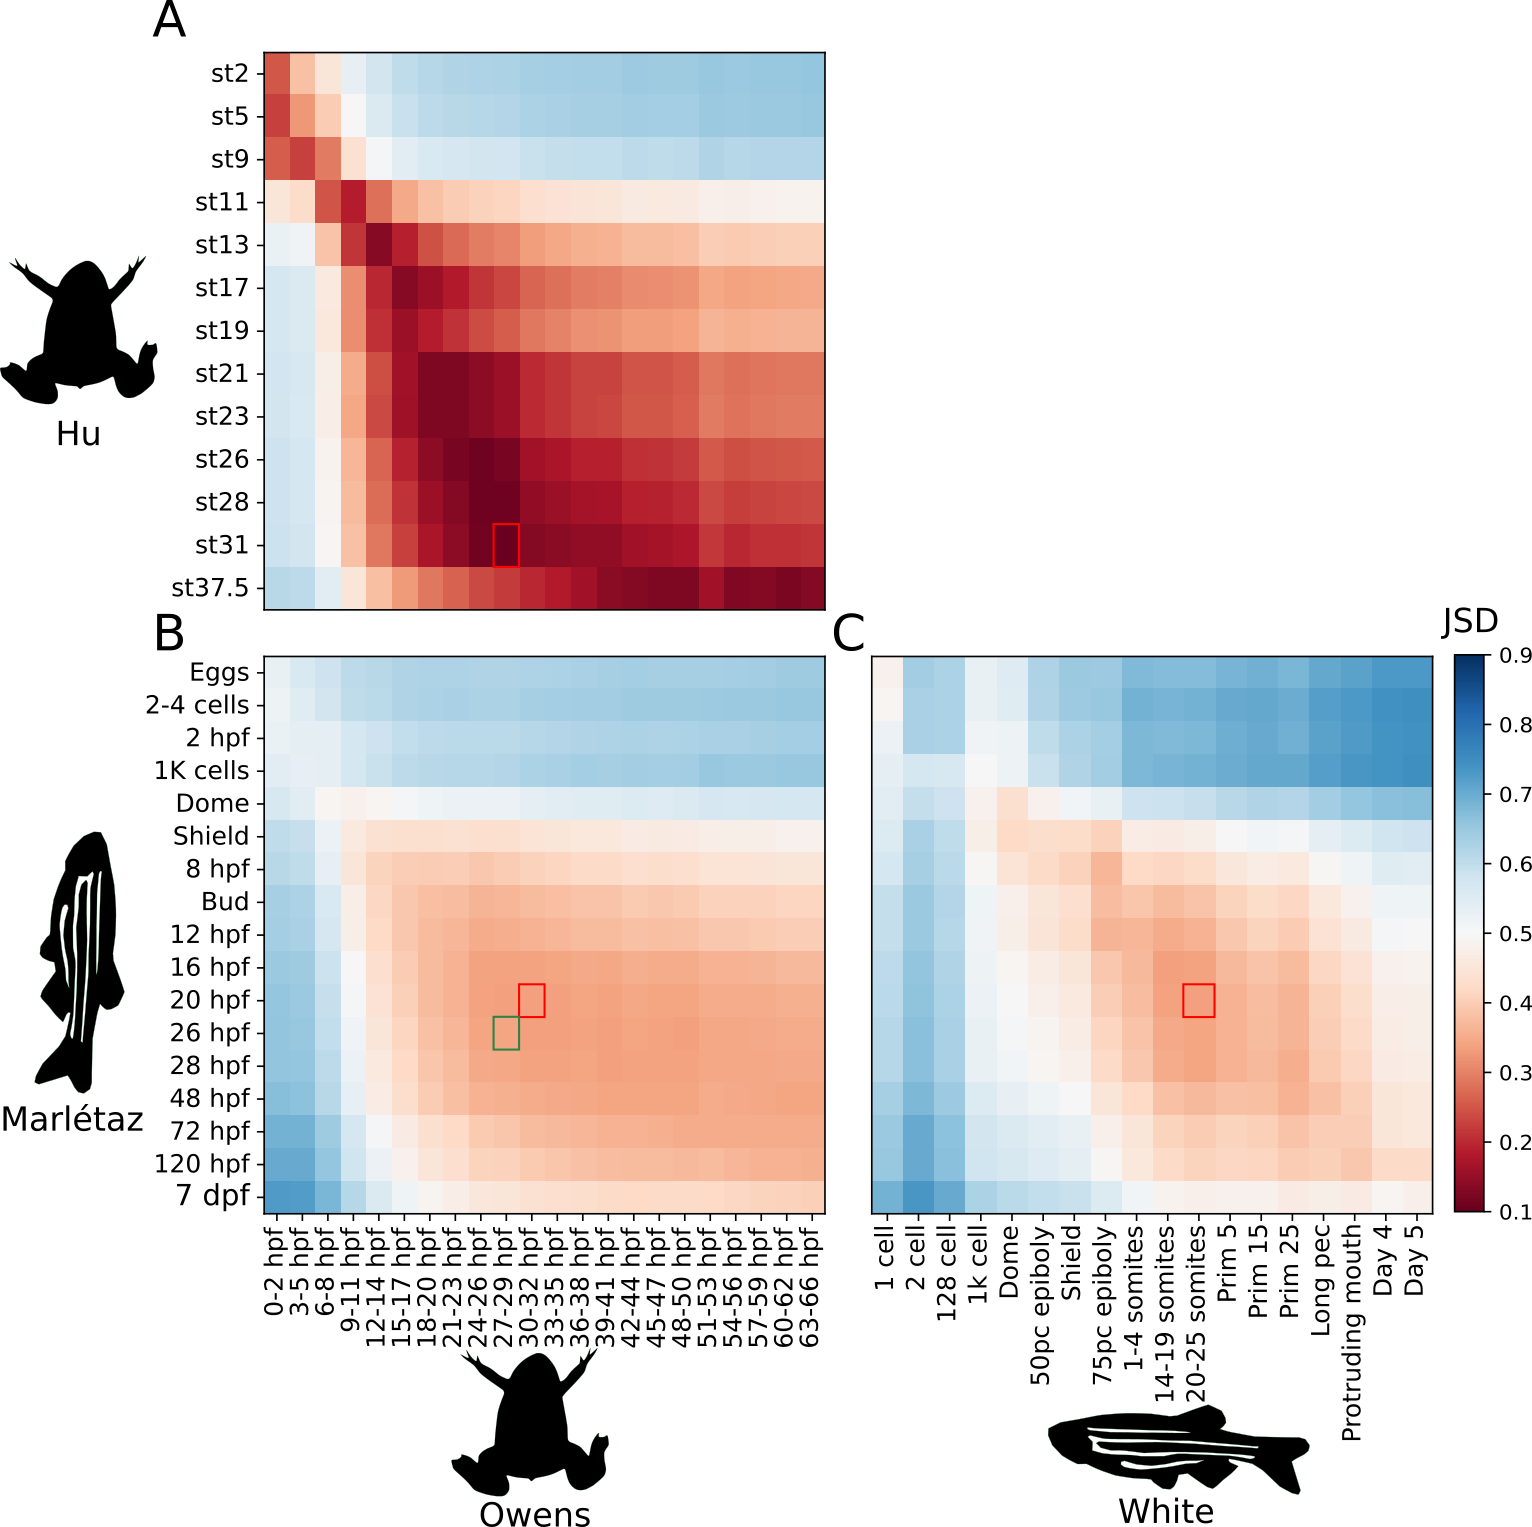
\includegraphics[width=\linewidth]{ch.hourglass/images/between_experiment.png}
    \caption{\textbf{Within species transcriptomic similarities translate to between species transcriptomic similarities}. Heatmap of pairwise Jensen-Shannon distances between \textbf{(A)} two \textit{Xenopus tropicalis} time series, \textbf{(B)} \textit{Xenopus tropicalis} and \textit{Danio rerio}, and \textbf{(C)} two \textit{Danio rerio} time series. The point of lowest Jensen-Shannon distance is marked in each comparison by a red square, and the green square represents the point of maximum similarity between \textit{Xenopus tropicalis} and \textit{Danio rerio} in the original study by Marl\'etaz et al.\cite{marletaz2018}. The between-species comparison seems to be a superimposition of the within-species effects.}
    \label{fig:betweenexperiment}
\end{figure}

Our re-analysis shows that an hourglass pattern already occurs in a within-species comparison of \textit{D. rerio} and \textit{X. tropicalis}. Any further comparison that is made between such time series suffers from this effect, and based on this re-analysis the between-species comparison can be explained as a superimposition of the two within-species patterns. This re-analysis does not exclude that the similarity between \textit{D. rerio} and \textit{X. tropicalis} at the phylotypic stage is higher than at other stages. All it shows is that without correction for within-species effects, we can not conclude whether certain embryonic stages are more or less conserved between species.

\subsection{The mid-developmental transition and the evolution of animal body plans} \label{subsection:levin}

In the paper \textit{The mid-developmental transition and the evolution of animal body plans}\cite{Levin2016} Levin \textit{et al.} compared the correlation coefficient of the expression of orthologous genes over time between ten species from different phyla. They found that most species-species comparisons had a high similarity early and late during development, with a period of low similarity during mid-development, which they called the \textit{mid-developmental transition}. They note that this period of low similarity between phyla seems to correspond to the phylotypic stage. They then suggest that this pattern could be used to distinguish different phyla. In this re-analysis, we demonstrate that we can find a \textit{mid-developmental transition} for both a within-phylum and between-phylum comparison. Moreover, we show that this pattern is a statistical artefact and can not be used to infer temporal conservational patterns.

Figure \ref{fig:within_phylum}A shows the pairwise Pearson correlation coefficient of one-to-one orthologs between each stage of \textit{Drosophila melanogaster} and \textit{Danio rerio}. With the same methodology as the original study, we get a dual-phase pattern where both the early and the late stages between the two species seem conserved, but with a period of low conservation in the middle. If we now apply the same methodology to the chordates \textit{D. rerio} and \textit{X. tropicalis}, we get a similar biphasic pattern, indicating the \textit{mid-developmental transition} is not exclusive to between phyla comparisons. Note that figure \ref{fig:within_phylum}B is based on the same sequencing data as figure \ref{fig:betweenexperiment}B. The reason that one shows an hourglass whilst the other an inverse hourglass is that gene standardization is applied to the inverse hourglass.

\begin{figure}[H]
    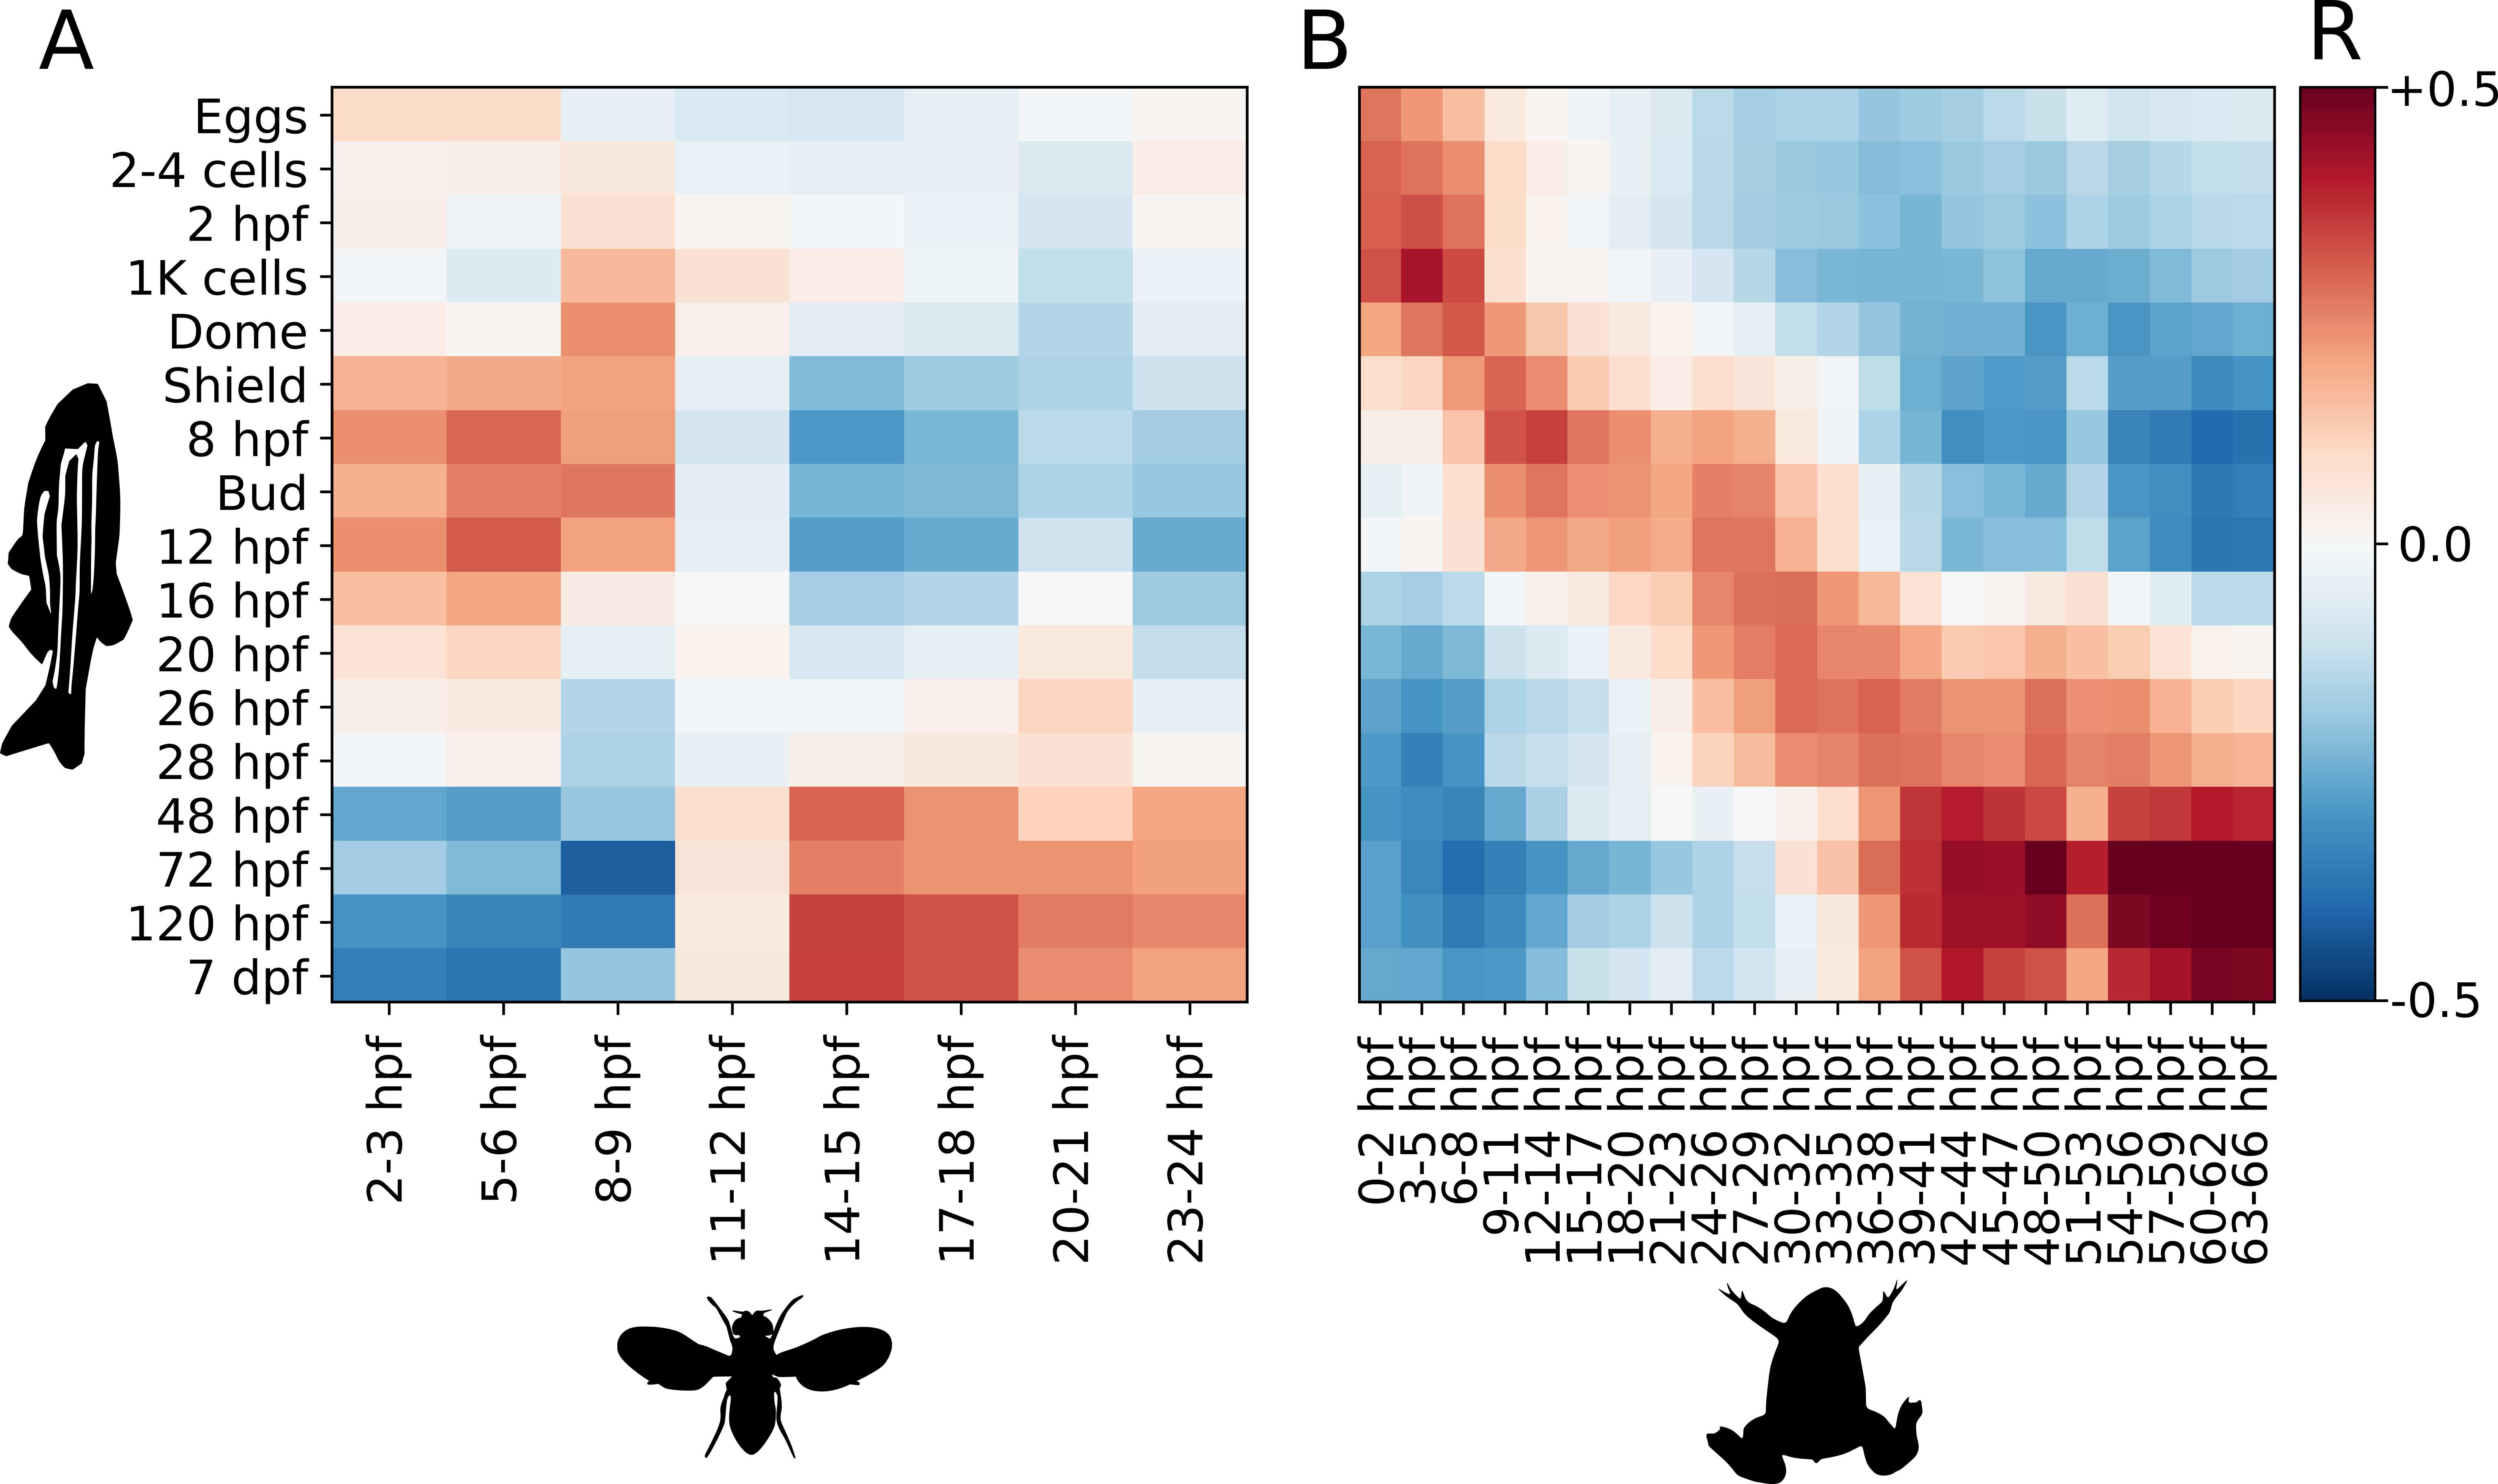
\includegraphics[width=\linewidth]{ch.hourglass/images/within_between_phyla.png}
    \caption{\textbf{The inverse hourglass is not exclusive to between phyla comparisons}. Heatmaps of pairwise Pearson correlation coefficients \textbf{(A)} for a between phylum comparison of \textit{Danio rerio} and \textit{Drosophila melanogaster}, and \textbf{(B)} a within phylum comparison of \textit{Danio rerio} and \textit{Xenopus tropicalis}. A mid-developmental transition is visible for both comparisons.}
    \label{fig:within_phylum}
\end{figure}

Levin \textit{et al.} apply gene standardization (z-score), which involves subtracting the mean and dividing by the standard deviation over time for each gene. Standardization is generally a good practice for parametric methods like the Pearson correlation coefficient. In the case of gene expression data, standardization effectively scales each gene to have equal weight in the correlation coefficient. Surprisingly, the use of standardization here leads to an unexpected side-effect. In the absence of standardization, the data exhibits an hourglass-like pattern (see fig. \ref{fig:standardization}A). However, after applying standardization, the pattern transforms into an inverse-hourglass shape. Even more surprising, we can cut each time series into four equal parts, and after standardization, three out of four comparisons still get a mid-developmental transition (fig. \ref{fig:standardization}B). 

\begin{figure}[H]
    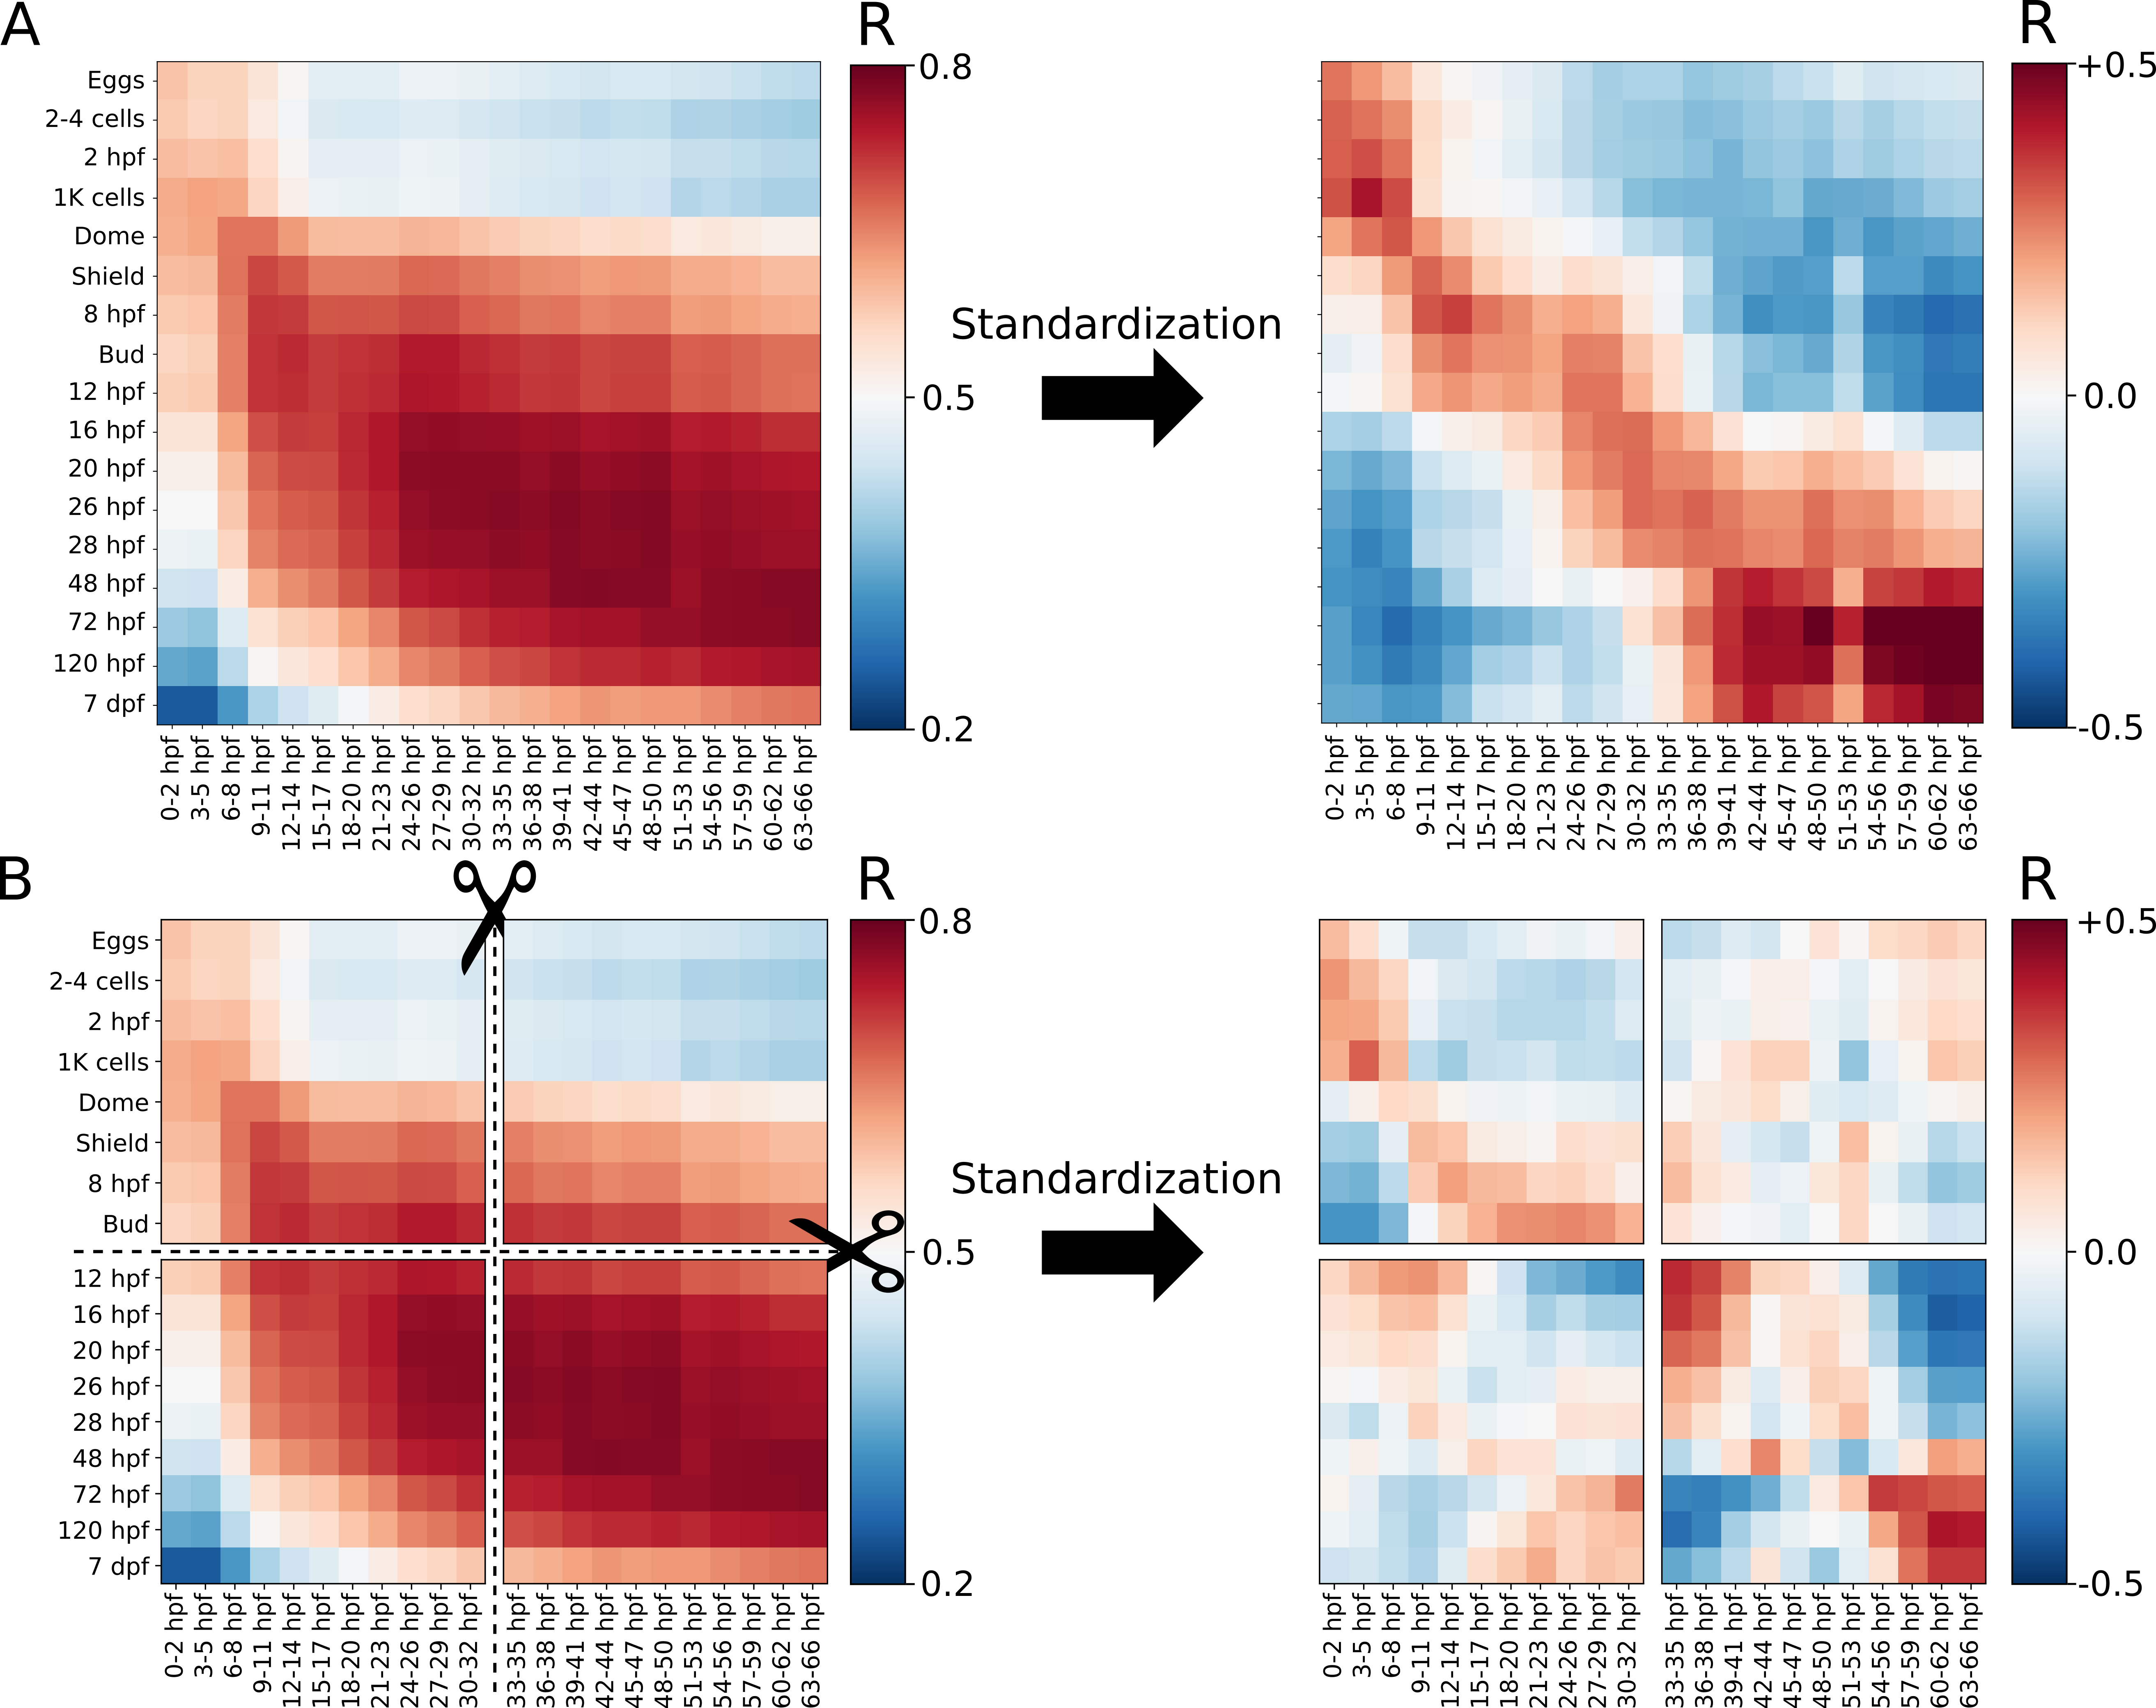
\includegraphics[width=\linewidth]{ch.hourglass/images/normalisation.png}
    \caption{\textbf{Heatmap of pairwise similarities between \textit{D. rerio} and \textit{X. tropicalis} and the effect of gene standardization}. \textbf{(A)} shows the effect of standardization. Before standardization an hourglass-like pattern is visible, whereas after standardization an inverse hourglass is visible. \textbf{(B)} shows the effect of standardization after dividing the pairwise into four equal parts. After standardizing each part, three out of four subsets now show an inverse hourglass. }
    \label{fig:standardization}
\end{figure}

To get an understanding as to why this happens we need to study the patterns of gene expression during development. One way to visualize gene expression patterns is a gene landscape, an approach coined by Levin \textit{et al}. The gene landscape is a histogram of the Pearson correlation coefficient for each gene with a linearly increasing line. A coefficient of 1 would mean that a gene is linearly going up over time, a coefficient of -1 would mean that a gene is linearly going down over time, and a coefficient of 0 would mean that a gene shows no linear temporal pattern. In figure \ref{fig:genelandscape} we show the gene landscape for \textit{D. rerio}, \textit{D. melanogaster}, and \textit{X. tropicalis}. For each species, we get an arc, with an enrichment for genes that are either going up or down over time, with relatively few genes having no linear temporal pattern. The scatterplot of Levin \textit{et al.} unfortunately hides this pattern, and a 2d histogram would have been a better choice. As embryo's grow one would expect practically all genes to get upregulated over time. But as RNA sequencing without spike-ins is inherently relative, genes are split into either one of two expression groups; a group where gene expression increases faster than the average gene (right side of the gene landscape) or the group where gene expression increases slower than the average gene (left side of the gene landscape). See figure \ref{fig:genelandscapenormalization} for the difference between per-embryo normalization and transcript per million (TPM) normalization for \textit{X. tropicalis} embryos.

\begin{figure}[H]
    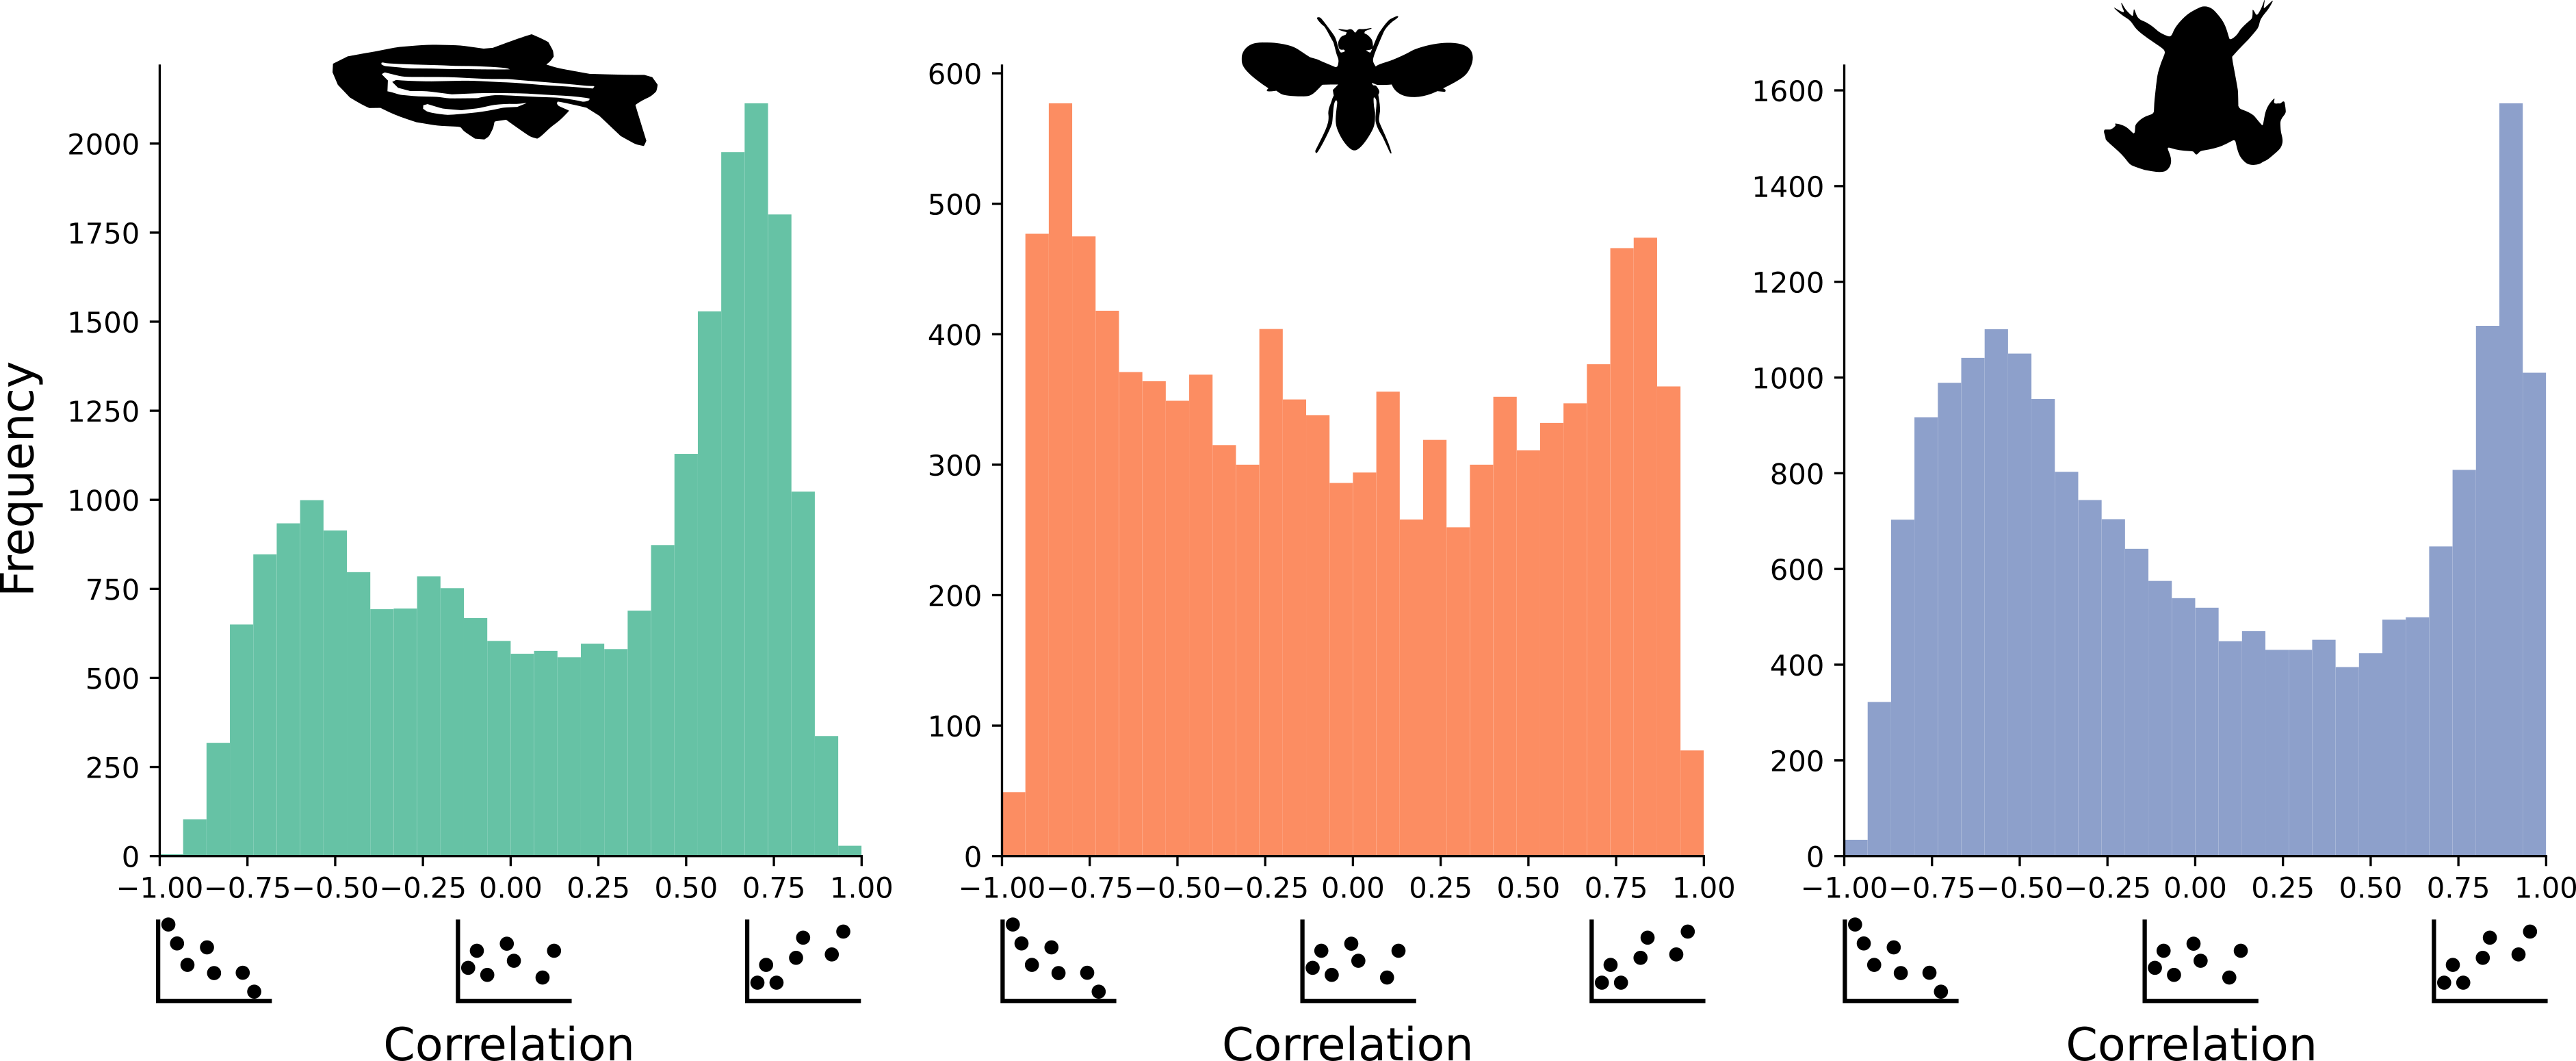
\includegraphics[width=\linewidth]{ch.hourglass/images/gene_landscape.png}
    \caption{\textbf{The gene landscape of \textit{D. rerio}, \textit{D. melanogaster}, and \textit{X. tropicalis} embryos}. The gene landscape is a histogram of each gene's correlation coefficient with a linearly increasing line. Note how generally speaking there are two groups of genes; a group of genes that is upregulated, and a group that is downregulated during embryonic development.}
    \label{fig:genelandscape}
\end{figure}

Now that we know that our genes can roughly be classified as either going up or going down over time, we can think about how this influences our analysis. Let's start by imagining the time-series of a single gene that has a binary expression profile, where at the start of our time-series the gene is \textit{off}, and at a random time point switches \textit{on} and stays on until the end of the series. We now imagine the expression profile of this gene in a related species and assume again that it starts \textit{off} and at random time point switches \textit{on}. We can express the probability that these two imaginary time-series are equal (section \ref{subsection:middevelopmenttransition}), and if we visualize these probabilities it is clear these odds show a mid-developmental transition (fig. \ref{fig:inverse_math}). This theoretical derivation is however an extreme oversimplification of what happens both biologically and analytically, and considers only a single gene. For this reason, we simulated two time-series with a continuous expression profile. In these series half of the genes start in an \textit{off} stage where expression is zero, and half in an \textit{on} where expression is one. Similarly to the thought experiment, these genes, at a random time-point, gradually switch from \textit{off} to \textit{on}, or vice versa (fig. \ref{fig:sim_explanation}A). We can now calculate the Pearson correlation coefficient between these simulated series, and again we get a clear mid-developmental transition. Similar to the biological data, if we cut the simulated data into halves, and apply standardization afterwards, we get a mid-developmental transition per subset of the data (fig. \ref{fig:sim_normalisation}). 

\begin{figure}[H]
    \includegraphics[width=\linewidth]{ch.hourglass/images/sim_explanation.png}
    \caption{\textbf{Simulated gene expression exhibits an inverse hourglass}. TODOOOO.}
    \label{fig:sim_explanation}
\end{figure}

By incorporating a within-phylum comparison it becomes clear that the mid-developmental transition is a statistical artefact of gene standardization. It can be considered a special case of Simpson's paradox, where by standardization gene expression gets put into two groups (high vs low expression). And even though there is no particular correlation within each group, there is a clear correlation when comparing the data set as a whole\cite{Saccenti2023}. This pattern is not caused by lowly expressed genes, as we applied the same criteria as Levin \textit{et al.} to only include dynamic genes (minimum expression of 10 and at least a log2 fold change). As such we see no molecular basis for an inverse hourglass model between phyla, which leaves the question as to how the phylotypic stage behaves in comparisons between-phyla wide-open.

\subsection{Time-aligned hourglass gastrulation models in rabbit and mouse} \label{subsection:mayshar}

In the paper \textit{Time-aligned hourglass gastrulation models in rabbit and mouse}\cite{Mayshar2023} Mayshar \textit{et al.} analyzed the similarity between developing rabbit and mouse embryo's on a single-cell level. One of the comparisons they make is how the correlation of cell type proportions between rabbits and mice changes over time. They observe an ``hourglass-like'' bottleneck of cell type proportions pre-gastrulation. In this re-analysis, we show that the observed bottleneck is caused by a rapid change of cell types of \textit{O. cuniculus}, and is unlikely to be caused by a between-species effect.

Figure \ref{fig:cellproportions} shows the pairwise Pearson correlation coefficient between cell type proportions of developing \textit{M. musculus} and \textit{O. cuniculus}. Figure \ref{fig:cellproportions}B is the between species comparison and shows the same result as the original paper. Mayshar \textit{et al.} describe this as a stereotypical pattern, where the beginning of development is aligned but not synchronized, leading to a bottleneck at approximately E7.5 followed by a more synchronized gastrulation process marked by cellular diversification. They conclude that around E7.5-E7.7, the narrowest point of the bottleneck, mouse and rabbit gastrulation are aligned with maximum specificity. However, looking at the within-species comparison of \textit{O. cuniculus} we see a similar bottleneck (figure \ref{fig:cellproportions}C). Before E7.5 the rabbit embryo consists of a small number of cell types, forcing the cell type distributions into two groups; a group of cell types that do not occur, and a group of cell types that do occur. From E7.7 on practically all cell types are present. All comparisons within \textit{O. cuniculus} before E7.5 give high correlation values, because in this case the Pearson correlation represents whether identical cell types are present. It says little about the correlation coefficient between cell types (known as Simpson's paradox \cite{Saccenti2023}). The bottleneck at E7.5 is caused by the rapid appearance of new cell types, something the current linear time scale can not cope with. Similar problems exist for the \textit{M. musculus} time series, but are less pronounced. These within species effects then get carried over to the comparison between \textit{M. musculus} and \textit{O. cuniculus}, leading to a misleading between species figure.

\begin{figure}[H]
    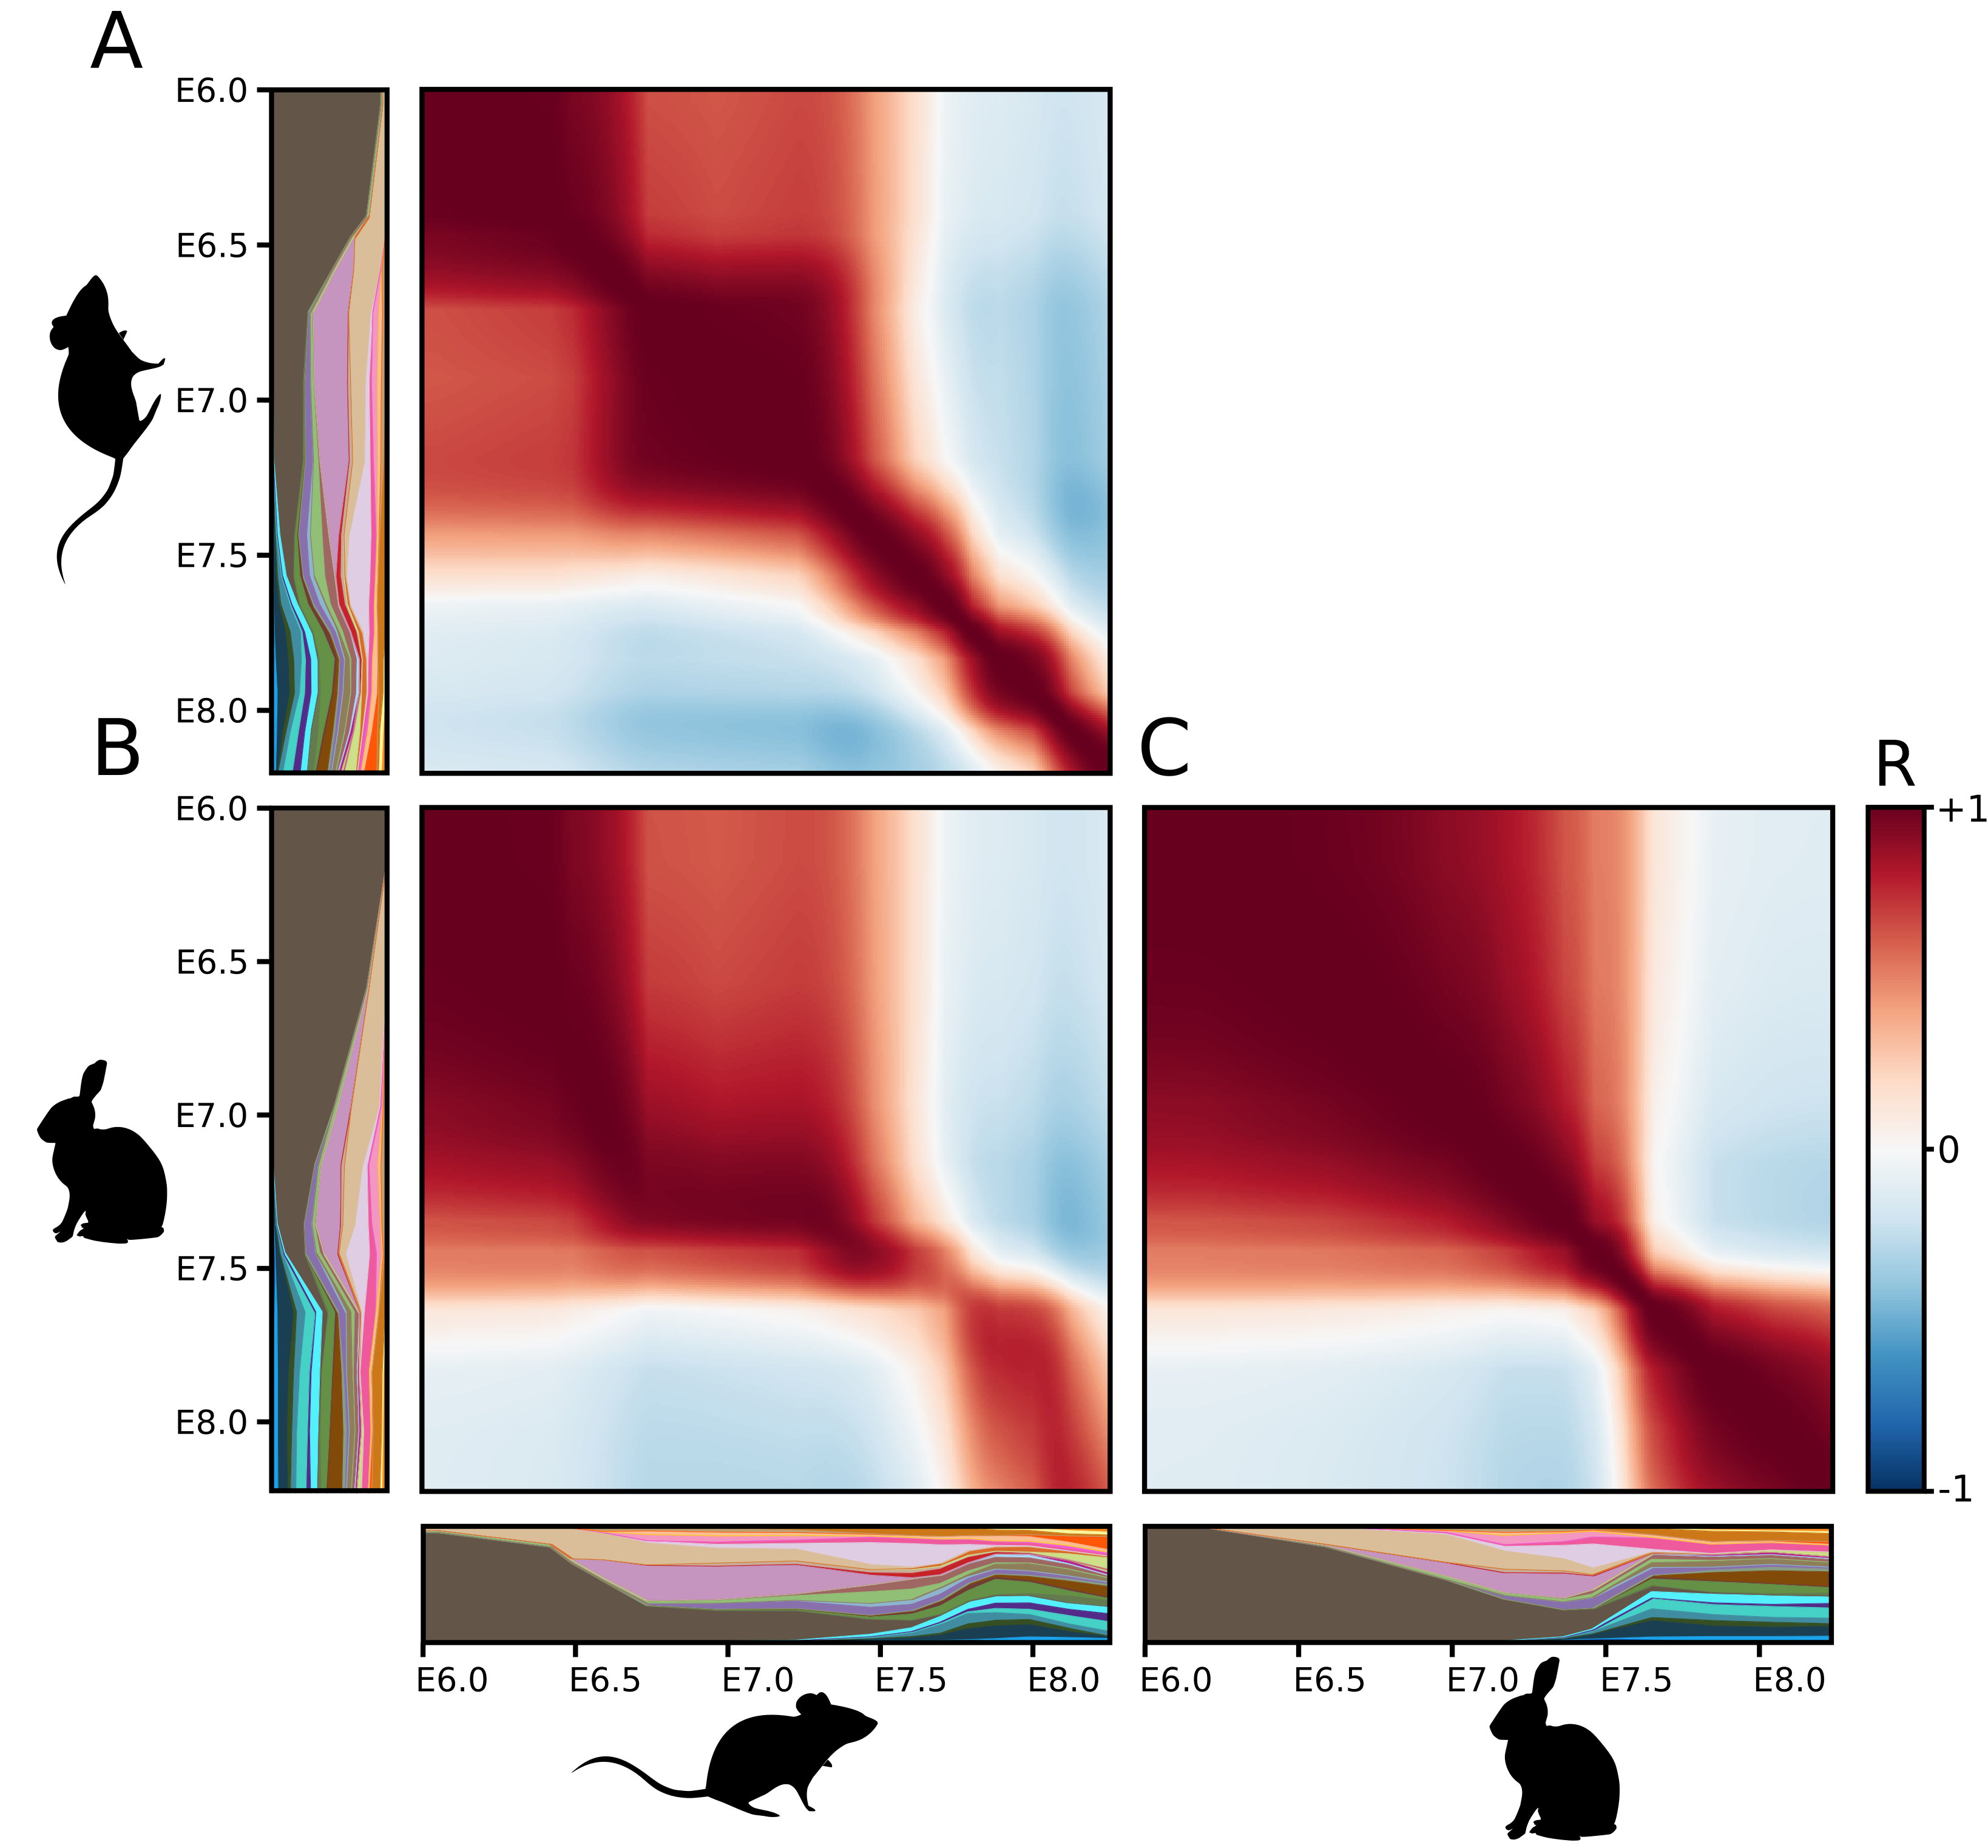
\includegraphics[width=0.8\linewidth]{ch.hourglass/images/mouse_rabbit_cellproportions.png}
    \caption{\textbf{Within-species cell type proportion similarities translate to between-species cell type proportion similarities}. Heatmap of pairwise Pearson correlation coefficients between \textbf{(A)} \textit{M. musculus} with itself, \textbf{(B)} \textit{M. musculus} and \textit{O. cuniculus}, and \textbf{(C)} \textit{O. cuniculus} with itself. The heatmaps are accompanied by cell type proportion charts with similar coloring as the original paper. The between-species pattern seems to be a superimposition of the within-species effects.}
    \label{fig:cellproportions}
\end{figure}

What is surprising about this analysis is that the pattern that Mayshar \textit{et al.} describe as a stereotypical pattern and hourglass-like, is neither stereotypical nor fits the hourglass model. For species of the same phylum no such sudden changes mid-development are expected. And the comparison in its current form actually displays a funnel pattern, with the highest similarity between \textit{M. musculus} and \textit{O. cuniculus} at the start of the time series which is gradually decreasing. Moreover, Mayshar \textit{et al.} conclude that their analysis shows that one can use absolute (linear) time for pairwise comparisons between gastrulating embryo's. But considering the within-species comparisons, we clearly see that the temporal axis is not representative of change. There is a higher rate of change happening between E7.5-E7.7 (5 hours) than between E6.0-E7.0 (24 hours). Altogether, the hourglass-like bottleneck between \textit{M. musculus} and \textit{O. cuniculus} seems to be caused by the within-species bottleneck, which in turn is partially caused by unrepresentative temporal sampling and a statistical artefact (Simpson's paradox).

\subsection{The hourglass model of evolutionary conservation during embryogenesis extends to developmental enhancers with signatures of positive selection} \label{subsection:liu}

In the paper \textit{The hourglass model of evolutionary conservation during embryogenesis extends to developmental enhancers with signatures of positive selection}\cite{Liu2021} Liu \textit{et al.} compare the similarity of accessible regions over five matched embryonic developmental time points between two \textit{Drosophila} species (\textit{D. melanogaster} and \textit{D. virilis}). Liu \textit{et al.} find that the middle time point (TP3) uses the most enhancers, and is the most conserved between these two flies (figure \ref{fig:peak_null}B). TP3 coincides with the \textit{Drosophila} phylotypic stage, and thus this result is seen as support for the hourglass model. In this re-analysis we show that the high conservation at the phylotypic stage is explained by the different number of enhancers found per time point, and is not a conservational pattern.

In this study, conservation is estimated by the similarity between time point specific enhancers between \textit{D. melanogaster} and \textit{D. virilis}. Time point specific enhancers are defined as enhancers that are enriched in only one time point (TP). Similarity is calculated by dividing the number of TP-specific enhancers present in both species simultaneously by the total number of TP-specific enhancers for both species (Jaccard index). Figure \ref{fig:peak_null}A shows the conservation over time between \textit{D. melanogaster} and \textit{D. virilis}, with the highest conservation at TP3. Figure \ref{fig:peak_null}B shows the number of  TP-specific enhancers per time point. The high amount of TP-specific enhancers at TP1 and TP5 can be explained by the fact that they are respectively the start and end of the time series. The high amount of TP specific enhancers at TP3, however, is not easily explained, and raises the question whether this can explain the high degree of similarity at TP3 between \textit{D. melanogaster} and \textit{D. virilis}. To investigate this potential bias we apply the same methodology between replicates from \textit{D. virilis}. We get a different conservational pattern, where TP1, TP3, and TP5 are most conserved between biological replicates (fig. \ref{fig:peak_null}C). Upon inspection it seems that the number of TP-specific enhancers between replicates seems positively correlated with the Jaccard index (fig. \ref{fig:peak_null}D). This indicates a potential bias in the methodology that needs further investigation.

To test whether a relationship between the number of TP-specific enhancers and Jaccard index exists, we've made a consensus set of enhancers for \textit{D. melanogaster} and \textit{D. virilis} over all time points. Each time point gets assigned a set of randomly picked enhancers, whilst keeping the number of enhancers per time point the same as originally found. This removes all biological meaning from the data, thus if the analysis is unbiased it should generate equal Jaccard indexes for all time points. Yet TP3 shows a clearly enriched Jaccard index (figure \ref{fig:shuffle}A). This proofs that the number of enhancers influences the analysis. The obvious way to control for this would be to subsample all time points to the same number of enhancers (figure \ref{fig:shuffle}B). After subsampling, we find that TP2, a different time point, shows the highest conservation between enhancers between \textit{D. melanogaster} and \textit{D. virilis}. The dependence of the Jaccard index on the number of enhancers can also be more formally proven, see section \ref{subsection:flypeaks}. 

\begin{figure}[H]
    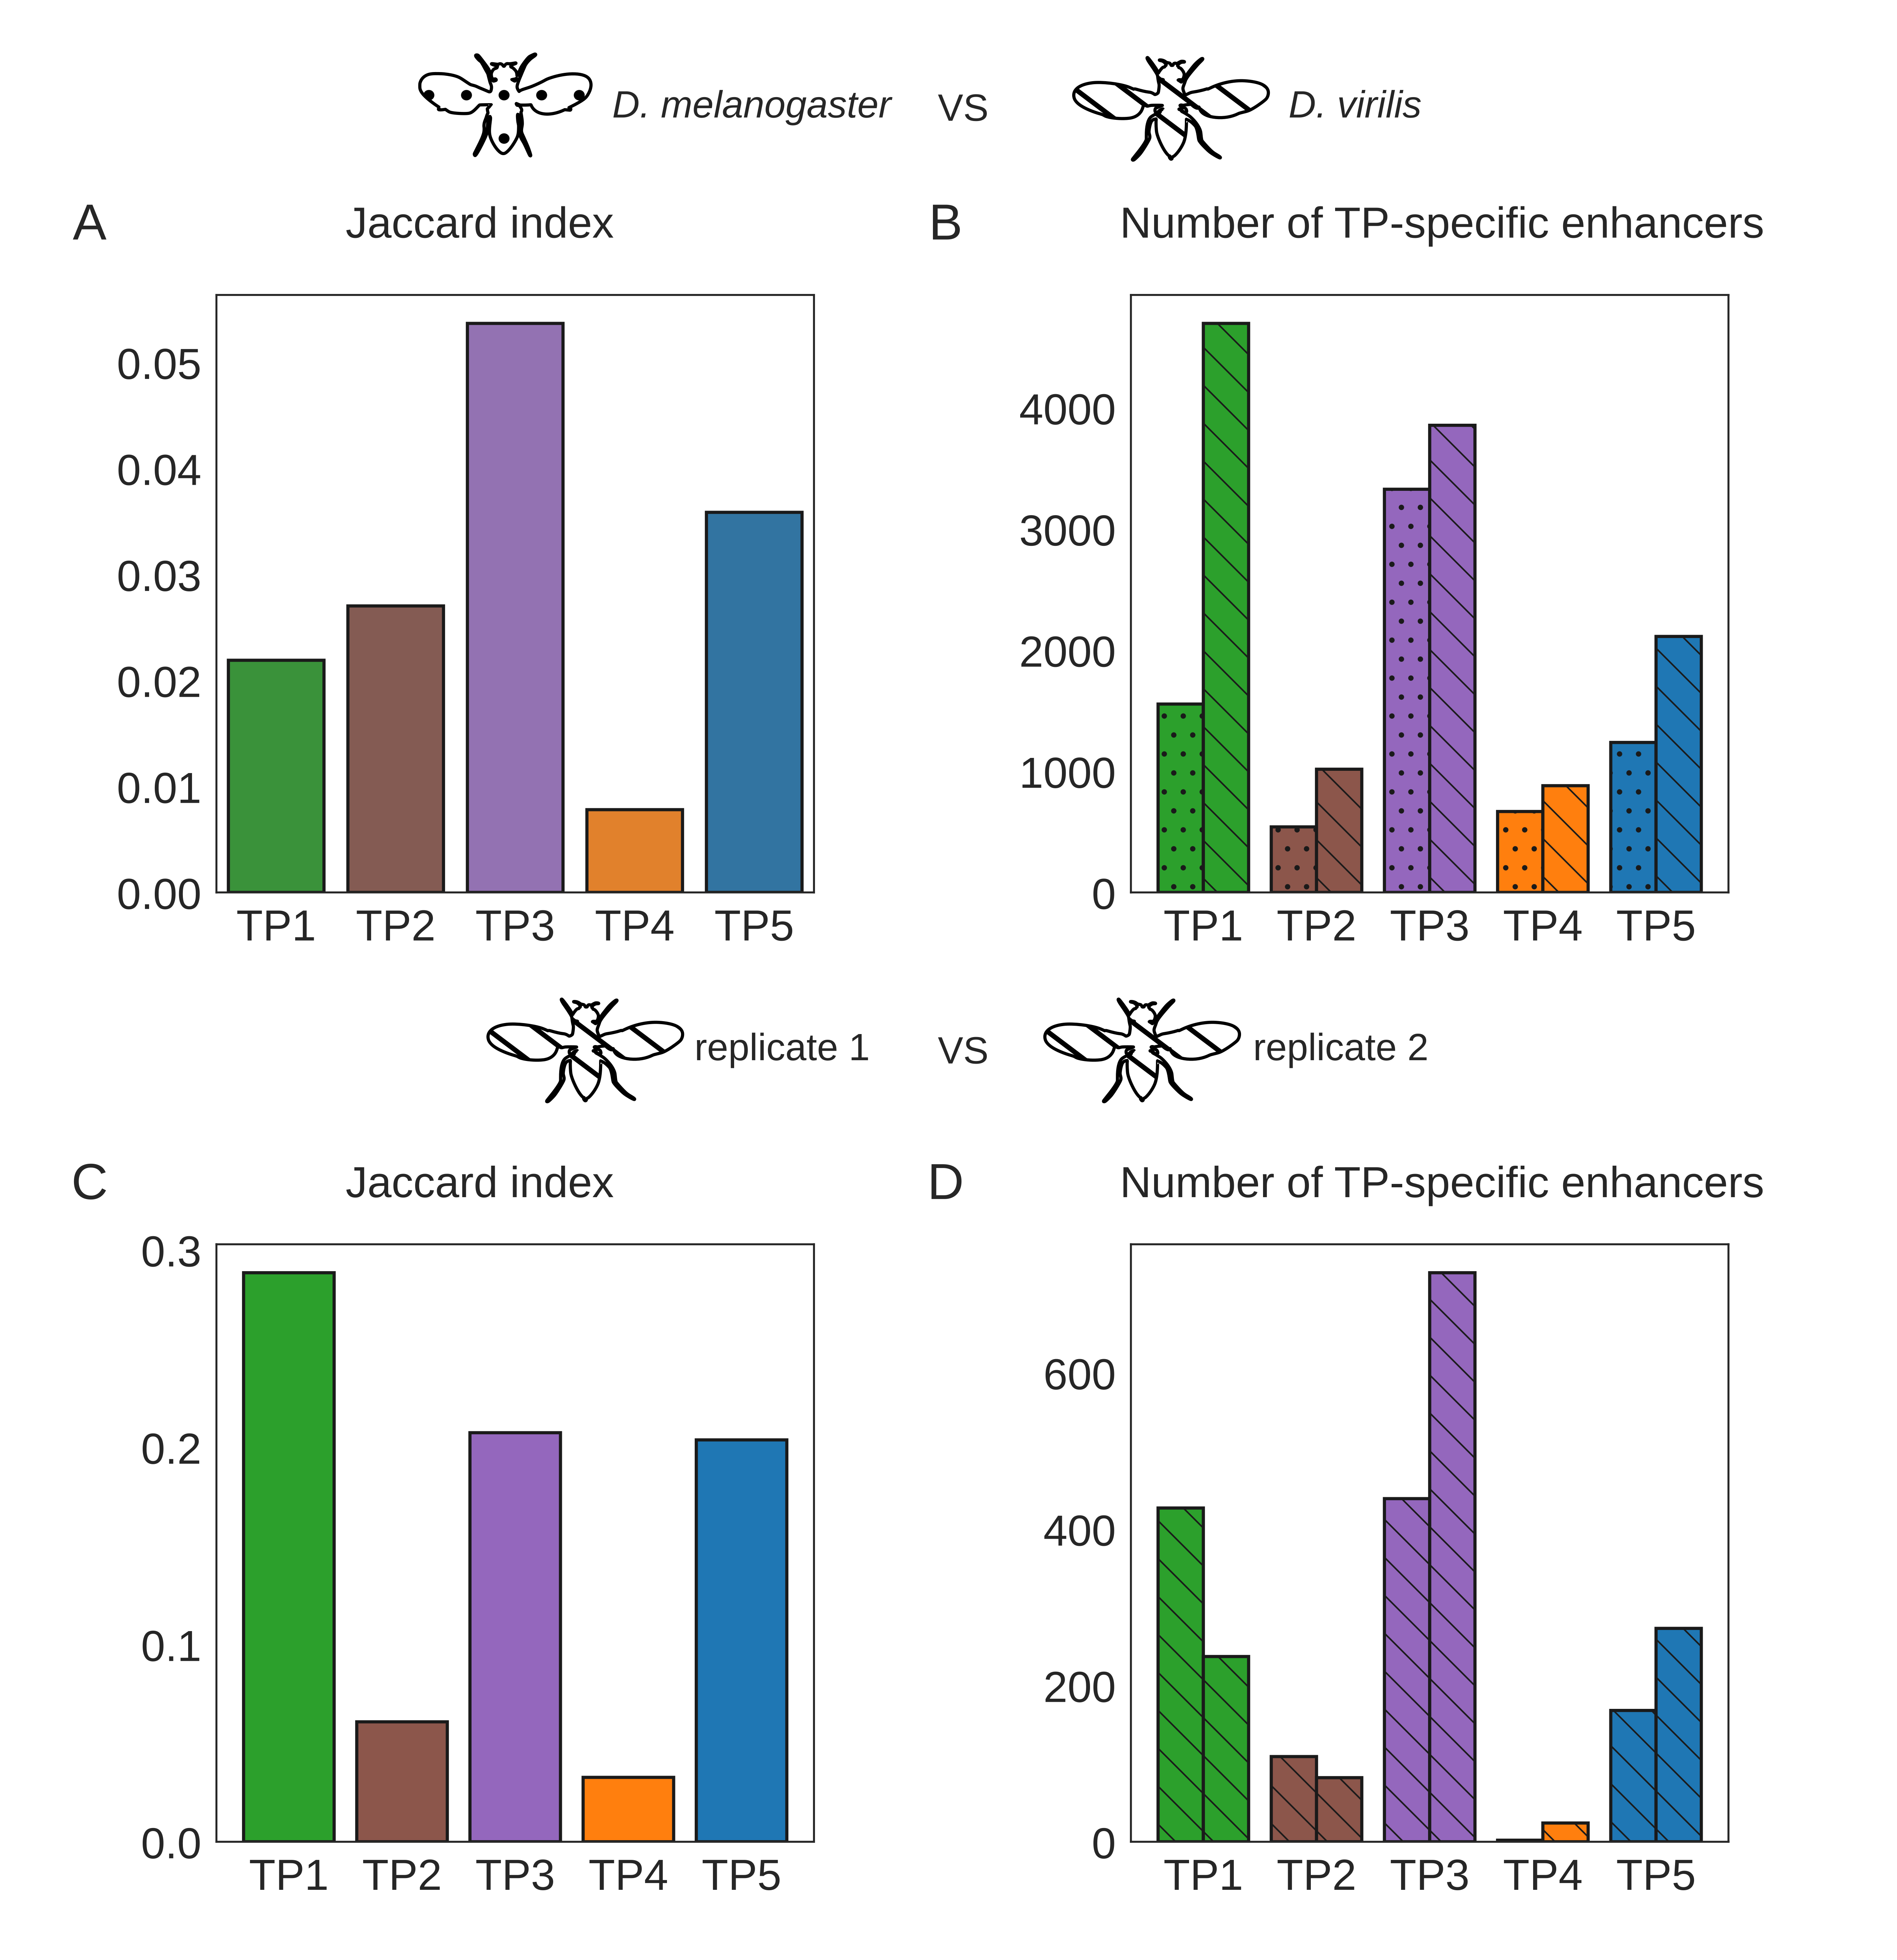
\includegraphics[width=\linewidth]{ch.hourglass/images/fly_control_2.png}
    \caption{\textbf{The dependency of the Jaccard index on the number of enhancers}. \textbf{(A)} Proportion of conserved stage-specific enhancers at each development stage between \textit{D. melanogaster} and \textit{D. virilis}. \textbf{(B)} The number of time point specific enhacers for \textit{D. melanogaster} and \textit{D. virilis} over time. \textbf{(C)} Proportion of conserved stage-specific enhancers at each development stage between replicates of \textit{D. virilis}. \textbf{(D)} The number of time point specific enhacers for \textit{D. virilis} replicates over time. }
    \label{fig:peak_null}
\end{figure}

\begin{figure}[H]
    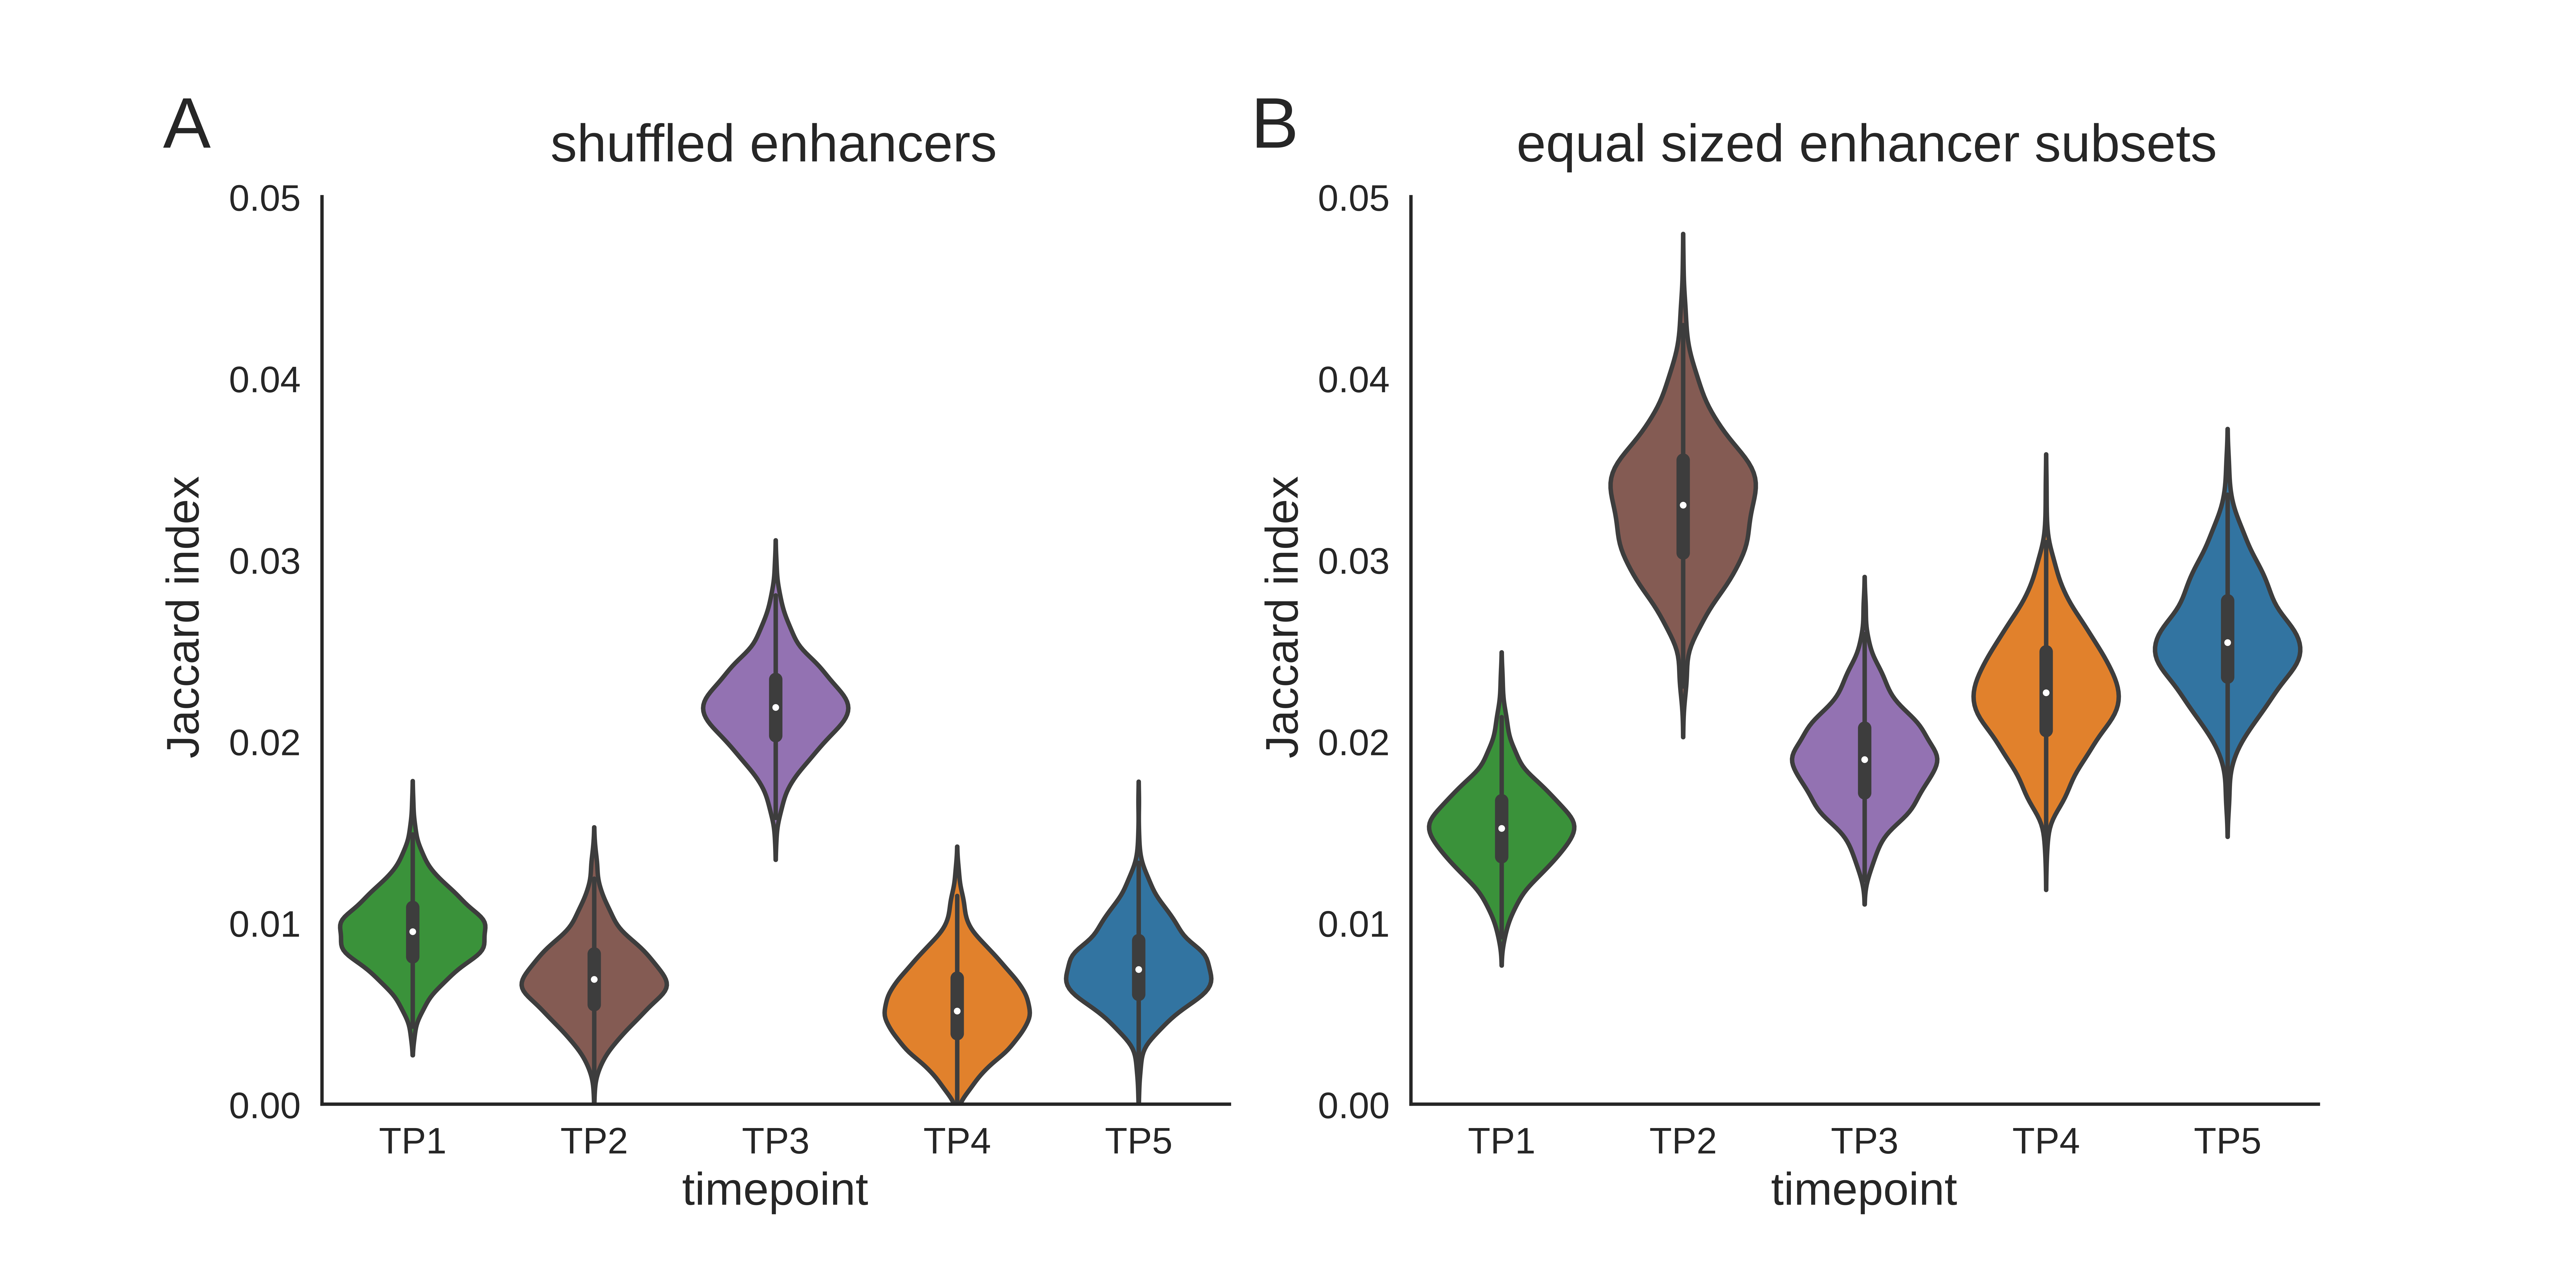
\includegraphics[width=\linewidth]{ch.hourglass/images/fly_shuffle.png}
    \caption{\textbf{Permutation tests show that the high similarity at the phylotypic stage is an artefact of the number of enhancers}. \textbf{(A)} Distribution of Jaccard scores after randomly distributing enhancers to time points, but with identical number of enhancers per time point as originally found. If the number of enhancers per time point does not influence the result an equal distribution is expected. The enrichment of TP3 however indicates that this methodology is sensitive to the number of enhancers per time point (TODO TP1: 100 TP2: 200 TP3: 300 TP4: 200 TP5: 100) . \textbf{(B)} Subsampling to TODO number of enhancers per time point. This removes the dependency of the Jaccard index on the number of enhancers. TP3 is clearly not enriched after subsampling.}
    \label{fig:shuffle}
\end{figure}

Apart from a biological interpretation for the different number of time-point specific enhancers, there are also two methodological interpretations. Firstly, the focus on TP-specific enhancers creates artificially separated sets of TP-specific enhancers. TP-specific enhancers are defined as occurring in one time-point only. This means that if two time-points are sampled more closely in time than other time-points, these two time-points would share most of their enhancers, resulting in a low number of TP-specific enhancers, something the authors themselves already note. Similarly, enhancers at the beginning and the end of the time-series have a higher chance of being TP-specific purely because they are only compared against one adjacent time-point whilst the rest of the time-series are compared against two. A similar approach is to visualize the percentage of reads in the consensus peak set in enhancers vs promoters per time point. Applied to this data we find no clear enrichment for enhancers for a specific time-point (fig. \ref{fig:peak_enrichment}). Secondly, arbitrary thresholds are used during peak calling to decide whether a region is \textit{enriched}. This threshold depends for instance on the signal-to-noise ratio, which is expected to change for a developing embryo, and the sequencing depth\cite{encode_guidelines2012}. Neither of these confounders have been corrected for in the original analysis.

Moreover, Liu \textit{et al.} proceed to train a computational model on the sequences of time-point specific enhancers of \textit{Drosophila melanogaster}. This model is then used to classify enhancers for whether they are subjected to positive selection. They then find that the ratio of enhancers subjected to positive selection vs enhancers subjected to non-positive selection is high for TP1, TP3, and TP5, and thus conclude that the molecular basis for the phylotypic stage can partially be explained by positive selection of gene regulation conservation. Alternatively, there are two other likely (methodological) explanations to this pattern. The first explanation is that as there has been no correction for signal-to-noise ratio and sequencing depth, there is a difference in the type(s) of peaks the pre-processing picked up, which in turn translates to different predicted positive selection ratios. The second explanation is that, as is true for practically all machine learning, the model generalizes and performs better with more training data. Looking at their reported model performance (AUC) we can clearly see that the model's performance for TP1, TP3, and TP5 is notably higher than for TP2 and TP4. Looking back at figure \ref{fig:peak_null}D we see that the high model performance closely follows the amount of training data (number of TP-specific peaks). Simply speaking, a model that has been trained with more data models predict a higher amount of positive selection. Without correction for these potential confounders it is hard to reach a definitive conclusion about positive selection with regards to the hourglass model and the phylotypic stage.

By comparing the within-species conservational pattern we expose important flaws in the experimental design of this study. Our re-analysis shows that the fact TP3 seems highest conserved between \textit{D. melanogaster} and \textit{D. virilis} is an effect of the number of TP-specific enhancers, and not because this time point is more conserved between these two species. Moreover it seems that the number of TP-specific enhancers also influences the downstream training of the gkm-SVM and in turn the pattern of enhancer positive selection. 

\section{Discussion}

Our study highlights the importance of including within-species, within-phylum, and between-phylum comparisons in the analysis of the phylotypic stage. We demonstrate that the high transcriptome similarity between \textit{D. rerio} and \textit{X. tropicalis} at the phylotypic stage and can be explained by within-species effects alone. Similarly, we show that the cell type proportion ``hourglass-like'' bottleneck is also caused by within-species effects. Furthermore, we identify the mid-developmental transition and \textit{Drosophila} enhancer conservation at the phylotypic stage as statistical artefacts. 

When comparing time-series directly, it is important to control for statistical biases in the data, such as the correspondence between replicates, but also the temporal sampling strategy, data distribution, cell type proportion, and gene sets used. A key bias that is often overlooked is whether the sampling schema follows developmental time\cite{BinindaEmonds2002}. It is not uncommon for studies to report a discontinuous blocked pattern of within-species conservation, where the difference between stages is not equal. This difference often gets assigned a biological explanation; for instance as embryonic genome activation\cite{Yanai2011} or developmental milestones\cite{Levin2012}. However, this blocked within-species pattern proceeds to affect the between-species comparison where the same blocks are visible. From a statistical point of view, the only way to make a fair comparison between time series is when the similarity between all adjacent time points is equal (or if one explicitly corrects this bias statistically). When sampling stages closely in time, one increases the probability of stages matching closely in a comparison with another time-series. This in turn increases the expected maximum similarity. The reverse is also true, where stages sampled in large intervals reduce the probability of matching stages between time-series, which then reduces the expected maximum similarity. Thus under the assumption that embryonic development has no point of higher selective pressure, a comparison between two time-series will have the highest expected similarity at the point where sampling has happened at the shortest interval. For this reason, we argue for a re-definition of molecular embryonic time, where not the morphological features or time post-fertilization is used, but where the (molecular) difference between adjacent stages is equal.

Similarly, changing gene expression distributions are an effect of developmental maturity\cite{Kannan2021}. Pluripotent tissues have relatively many genes activated, whilst more mature tissues make use of a smaller more specialized set of genes. These changing gene expression distributions over time can introduce unexpected biases and artefacts when calculating similarity. For instance, the JSD and Pearson correlation coefficient between two count tables from different distributions can respectively never be zero or one. As an effect, directly comparing similarity scores between time-points can be misleading as the range of possible similarity scores is different per comparison. To circumvent this problem one can resort to non-parametric distance metrics, such as the rank-based Spearman correlation coefficient\cite{Irie2011}, or quantile normalizing the data before calculating the distance metric\cite{marletaz2018}. Then, one can compare the similarity scores directly, but these approaches ignore the biologically relevant gene expression distribution changes. As long as there is no consensus on what type of molecular similarity is expected at the phylotypic stage, it can both be correct as well as incorrect to ignore the distributional changes. 

Another point to consider is the changing proportions of cell types. An embryo is formed by all the multiplying and developing cells together, and their combined signal is measured in the study of the molecular phylotypic stage. But not every cell type expresses the same amount of transcripts\cite{Kim2023, Percharde2017}, which consequently gives cells with a lot of transcripts a higher importance in the (dis)similarity calculation. Moreover, molecular changes embryonic similarity between species could be either caused by changes in gene expression, or by changes in cell proportions. For example, during the vertebrate phylotypic stage the neural tissue is already highly developed and relatively large. Perhaps similarity at the vertebrate phylotypic stage is an effect of the over-representation of these neural cell types? Or as another example, a practically universal feature of embryos is that they grow during development. But because of this growth, for example, the surface (skin) to volume (organs) ratio changes, which could be another driving force for the molecular phylotypic stage. We currently do not understand whether the molecular similarity at the phylotypic is based on cell type proportion similarity or whether it is based on gene expression similarity. Only a single-cell approach can distinguish the effects of cell type proportion and gene expression, which is essential for better understanding the molecular phylotypic stage.

Moreover, calculating a single similarity score between species seems like a gross oversimplification of the complexity of evolutionary development. When focusing on one-to-one orthologues features, all newly derived and lost features are ignored. For instance, we started our analysis with 21.154 genes for \textit{X. tropicalis} and 24.417 genes for \textit{D. rerio} respectively. However, if we focus only on one-to-one orthologs this gets reduced to 5.444 genes. This means that for this comparison specifically, we discard approximately three-quarters of the biological signal. To our knowledge, the only method that considers these relations is the transcriptomic derivedness index\cite{Leong2021}. Moreover, gene expression is regulated by the complex interplay of multiple gene regulatory mechanisms. For instance, a single differentially expressed transcription factor can affect thousands of downstream genes. Biological data is notoriously not independently and identically distributed (iid). Whole-transcriptome comparisons are thus biased towards the largest groups of co-regulated genes. In addition, the fact that comparisons subsetted on different GO terms result in different conservational patterns is a clear indication that a single metric for whole-transcriptome similarity conceals the different layers of conservation at the phylotypic stage\cite{Malik2017,Gildor2019,Onimaru2021}.

Even though there has been extensive research into the molecular basis of the phylotypic stage, there is currently no clear hypothesis for it. There is no pre-defined expectation when comparing members of different phyla, nor has it been defined whether the similarity between species of the same phylum is a between-species or within-species effect. It is unclear whether high similarity is expected as a generic gene expression similarity(dynamic pattern), or whether the high similarity expresses itself as highly conserved gene regulation(gene regulatory complexity). Without explicitly testing these different possibilities we can not fully appreciate and understand the complexity of evolutionary embryonic development. Moreover, we do not feel that the current whole-embryo pairwise comparisons are a sincere attempt to understand evolutionary development, but instead are applied because they are simplest to measure. 

Deliberately have not shown more extensive comparisons within, between, etc. As it is important to define.

\section{Material and Methods}

The final analysis can be found on https://github.com/vanheeringen-lab/phylotypic\_hourglass.

\subsection{Transcriptome analyses}

Preprocessing of RNA-seq was done automatically by seq2science v0.9.8\cite{seq2science} using the rna-seq workflow. Public samples were downloaded from the Sequence Read Archive with help of the ncbi e-utilities and pysradb\cite{Choudhary2019}. Genome assemblies UCB\_Xtro\_10.0 (\textit{X. tropicalis}), GRCz11 (\textit{D. rerio}), BDGP6.32 (\textit{D. melanogaster}), ce11 (\textit{C. elegans}) and GRCm38.p6 (\textit{M. musculus}) were downloaded with genomepy 0.13.0\cite{Frlich2023}. Reads were trimmed with fastp v0.20.1\cite{Chen2018} with default options. Reads were aligned with STAR v2.7.6a\cite{Dobin2012} with default options. Afterwards, duplicate reads were marked with Picard MarkDuplicates v2.23.8\cite{picard}. General alignment statistics were collected by samtools stats v1.14\cite{Danecek2021}. Read counting and summarizing to gene-level was performed on filtered bam using HTSeq-count v0.12.4\cite{Anders2014}. TPM normalized gene counts were generated using genomepy based on longest transcript lengths. Quality control metrics were aggregated by MultiQC v1.14\cite{Ewels2016}. 

The within-species permutation test was performed by randomly choosing two replicates of the same time-point and calculating their Spearman correlation coefficient, with per time point 250 random pairs.

Orthologs between species were derived by the gimmemotifs motif2factors command. This command downloaded the genome assemblies of TODO X Y Z through genomepy\cite{Frlich2023}, and converted all transcripts to peptides with gffread 0.12.7\cite{Pertea2020}. Only the longest peptide per gene was kept, which were then fed to orthofinder 2.5.4\cite{Emms2019}.

For the re-analyses we then took the average TPM per time point, kept per species-species comparison only the one-to-one orthologs, and did similar processing as the original studies. Specifically for the re-analysis of Marl\'etaz \textit{et al.} we quantile normalized\cite{qnorm} the TPMs and calculated the Jensen-Shannon distance on a log2 scale with TPMs divided by a million. The absolute JSD values are however vastly different between our and the original analysis, which is because we have opted to represent TPMs as probabilities and calculate JSD using a log base of 2. This causes the JSD to be bound between 0 and 1, which makes comparisons between different data sets easier as they are on the same scale. For the re-analysis of Levin \textit{et al.} we removed all genes with a minimum TPM lower than 10 and less than a 10-fold change. Then we log10 transformed the remaining data and calculated the Pearson correlation coefficient.

\subsection{Enhancer conservation}

We've had trouble closely reproducing the original results of Liu \textit{et al.}, so we've opted to use the original processed data for the between-species comparison, but our own processed data for the within-species comparisons as this data is missing. By closely reproducing the original results with their data it shows that our ortholog inference works similarly to theirs.

Preprocessing of the within-species comparisons was done automatically by seq2science v0.9.8\cite{seq2science} using the atac-seq workflow\cite{Choudhary2019}. Genome assemblies \textit{dm6} and \textit{droVir3} were downloaded with genomepy 0.13.0\cite{Frlich2023}. Paired-end reads were trimmed with fastp v0.20.1\cite{Chen2018} with default options. Reads were aligned with bwa-mem2 v2.2.1\cite{bwamem2} with options '-M'. Afterwards, duplicate reads were marked with Picard MarkDuplicates v2.23.8\cite{picard}. Before peak calling, paired-end info from reads was removed with seq2science so that both mates in a pair get used. The peak-calling effective genome size was estimated by khmer v2.0\cite{Crusoe2015} by calculating the number of unique k-mers with k being the average read length per sample. Peaks were called with macs2 v2.2.7\cite{Zhang2008} with options '--shift -100 --extsize 200 --nomodel --buffer-size 10000' in BAM mode. A consensus set of all summits was made with gimmemotifs 0.17.2\cite{gimmemotifs}. We've removed all summits that fall within a TSS with pyranges v0.0.120\cite{Stovner2019}.

For the between-species comparison we've used pslmap to map all \textit{droVir3} enhancers to the \textit{dm6} assembly and only kept one-to-one orthologous regions. For the within-species comparisons this is not necessary. Time-point specific enhancers are defined as enhancers of which the summits are more than 200 base pairs removed from the enhancers of other time-points. Overlap over time is calculated as the Jaccard index.

\section{Acknowledgements}

We would like to thank Jialin liu for his quick response on queries about the \textit{Drosophila} transcriptome datasetm, Eileen Furlong for her help with processing the DNAse \textit{Drosophila} samples, Michal Levin and Itai Yanai for sharing their original orthology dataset, David Emms for help with questions about orthofinder. Mike Keesey for developing Phylopic, and Eivind Fonn for his help with formalizing the mathemathical derivations.

\section{Supplementals}

\subsection{mid-developmental transition derivation}\label{subsection:middevelopmenttransition}

A basic proof that the mid-developmental transition is a methodological artefact follows relatively easily from the thought experiment where a gene starts the time-series in an \textit{off} state, and at random switches to an \textit{on} state somewhere along this time-series:

\begin{align*}    
    G(t) & = \begin{cases} \text{off},& t < t_{\text{activate}} \\ \text{on},& t \geq t_{\text{activate}} \end{cases} \quad \textrm{and} \quad
    t_{\text{activate}} = \text{Uniform}(0, 1) \quad \textrm{and} \quad
    0 \leq t \leq 1
\end{align*}

then:

\begin{align*}
    P(G(t) & = \text{on}) = t \\
    P(G(t) & = \text{off}) = 1 - t
\end{align*}

If we now assume we have two of these time-series (x and y), we can define the probabilities that both genes are in the same state for $t_x$ and $t_y$:

\begin{align*}
    P(G(t_x) = G(t_y)) & = P(G(t_x) = \text{on}) \cdot P(G(t_y) = \text{on}) + P(G(t_x) = \text{off}) \cdot P(G(t_y) = \text{off}) \\
    & = t_x \cdot t_y + (1 - t_x) \cdot (1-t_y)
\end{align*}

When visualizing the probability for equality over all x and y a mid-developmental transition becomes clear (fig. \ref{fig:inverse_math}).

\subsection{Jaccard index}\label{subsection:flypeaks}

We assume that all enhancers are conserved between species $x$ and $y$. Moreover we assume that our pre-processing randomly finds enhancers for each time-point with chance $\alpha_{ts}$, where $t$ represents the time-point and $s$ represents the species. We can calculate the number of time-point specific peaks for $U_{ts}$ in this case as:

\begin{align*}
    E & \text{ is the collection of all conserved enhancers between species } x \text{ and } y \\
    U_{ts} & \text{ represents the time-point specific enhancers for species } s \text{ at time point } t \\
    |U_{ts}| & = \alpha_{ts} \beta_{ts} |E|, \text{ where } \beta_{ts} = \prod_{i \in \{1, 2, 3, 4, 5\}\setminus\{t\}} (1 - \alpha_{is}) \\
\end{align*}

Where $\beta_{ts}$ represents the fraction of enhancers that have are still eligible to be time-point specific. We can now calculate the expected overlap (union) between two time-points of species $x$ and $y$:

\begin{align*}
    \mathbb{E}(|U_{tx} \cap U_{ty}|) & = |U_{tx}| * \frac{|U_{ty}|}{|E|} \\
    & = \alpha_{tx} \beta_{tx} |E| * \frac{\alpha_{ty} \beta_{ty} |E|}{|E|} \\
    & = \alpha_{tx} \beta_{tx} \alpha_{ty} \beta_{ty} |E| \\
\end{align*}

From this we can calculate the expected Jaccard index:

\begin{align*}
    Jaccard(U_{tx}, U_{ty}) & = \frac{|U_{tx} \cap U_{ty}|}{|U_{tx} \cup U_{ty}|} \\
    & = \frac{|U_{tx} \cap U_{ty}|}{|U_{tx}| + |U_{ty}| - |U_{tx} \cap U_{ty}|} \\
    & = \frac{\alpha_{tx} \beta_{tx} \alpha_{ty} \beta_{ty} |E|}{(\alpha_{tx} \beta_{tx} + \alpha_{ty} \beta_{ty} - \alpha_{tx} \beta_{tx} \alpha_{ty} \beta_{ty})|E|} \\
    & = \frac{\alpha_{tx} \beta_{tx} \alpha_{ty} \beta_{ty}}{\alpha_{tx} \beta_{tx} + \alpha_{ty} \beta_{ty} - \alpha_{tx} \beta_{tx} \alpha_{ty} \beta_{ty}}
\end{align*}

For simplicity we assume that all found enhancers are time-point specific ($\beta_{ts} = 1$), simplifying the formula to:

\begin{align*}
    Jaccard(U_{tx}, U_{ty}) & = \frac{\alpha_{tx} \alpha_{ty}}{\alpha_{tx} + \alpha_{ty} - \alpha_{tx} \alpha_{ty}}
\end{align*}

We can now visualize the Jaccard index for different $\alpha_{ts}$ values and can see a clear dependence on the fraction of enhancers found and the Jaccard index (fig. \ref{fig:peak_math}). From this it is clear that we need to correct for the number of enhancers. $\beta_{ts}$ only influences the height of the Jaccard index, but not the pattern.

\subsection{supplemental figures}
\beginsupplement

\begin{figure}[H]
    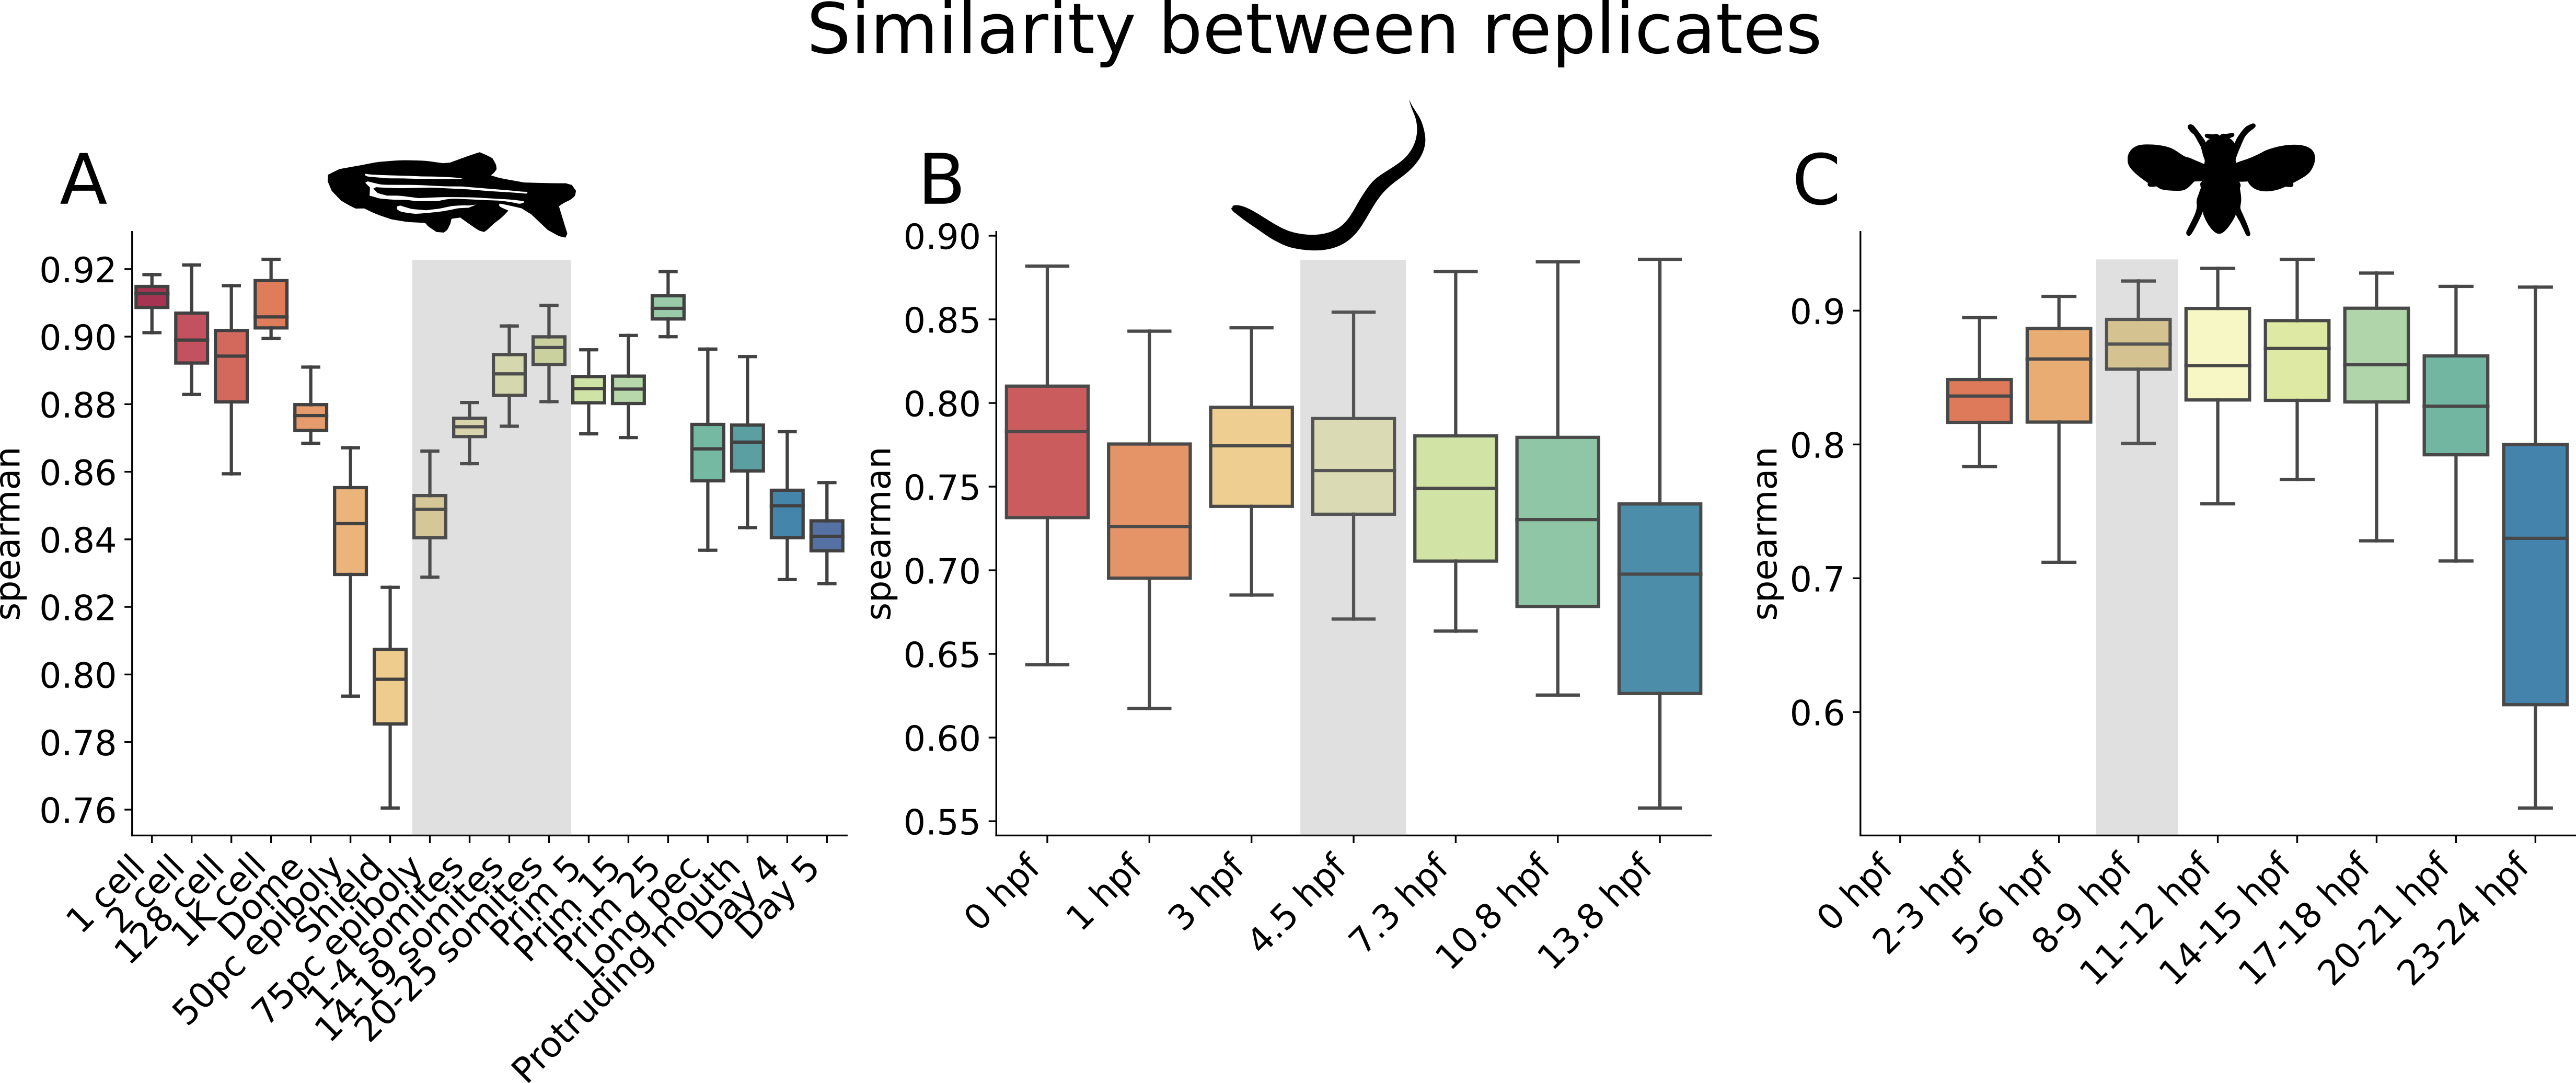
\includegraphics[width=\linewidth]{ch.hourglass/images/within_timepoint.png}
    \caption{\textbf{Changing levels of similarity between replicates is a potential cause for bias.} Boxplots of gene expression Spearman correlation coefficients between replicates belonging to the same stage for (A) single embryo \textit{D. rerio} samples, (B) pools of 10 \textit{C. elegans} embryos, and (C) single-embryo \textit{D. melanogaster} samples. The data is based on 250 randomly sampled pairs of replicates. The shaded area indicates the phylotypic stage. Note that all three species display a seemingly similar pattern, with a high similarity between replicates at the start and mid-development. And a drop early and late development. There are many potential causes for the changing levels of similarity over time; more biological variation between replicates at certain stages, a stage spanning too much time or inversely a rapid development during certain stages, lab protocols that are optimized for certain stages and not others, etc.}
    \label{fig:within_timepoint}
\end{figure}

\begin{figure}[H]
    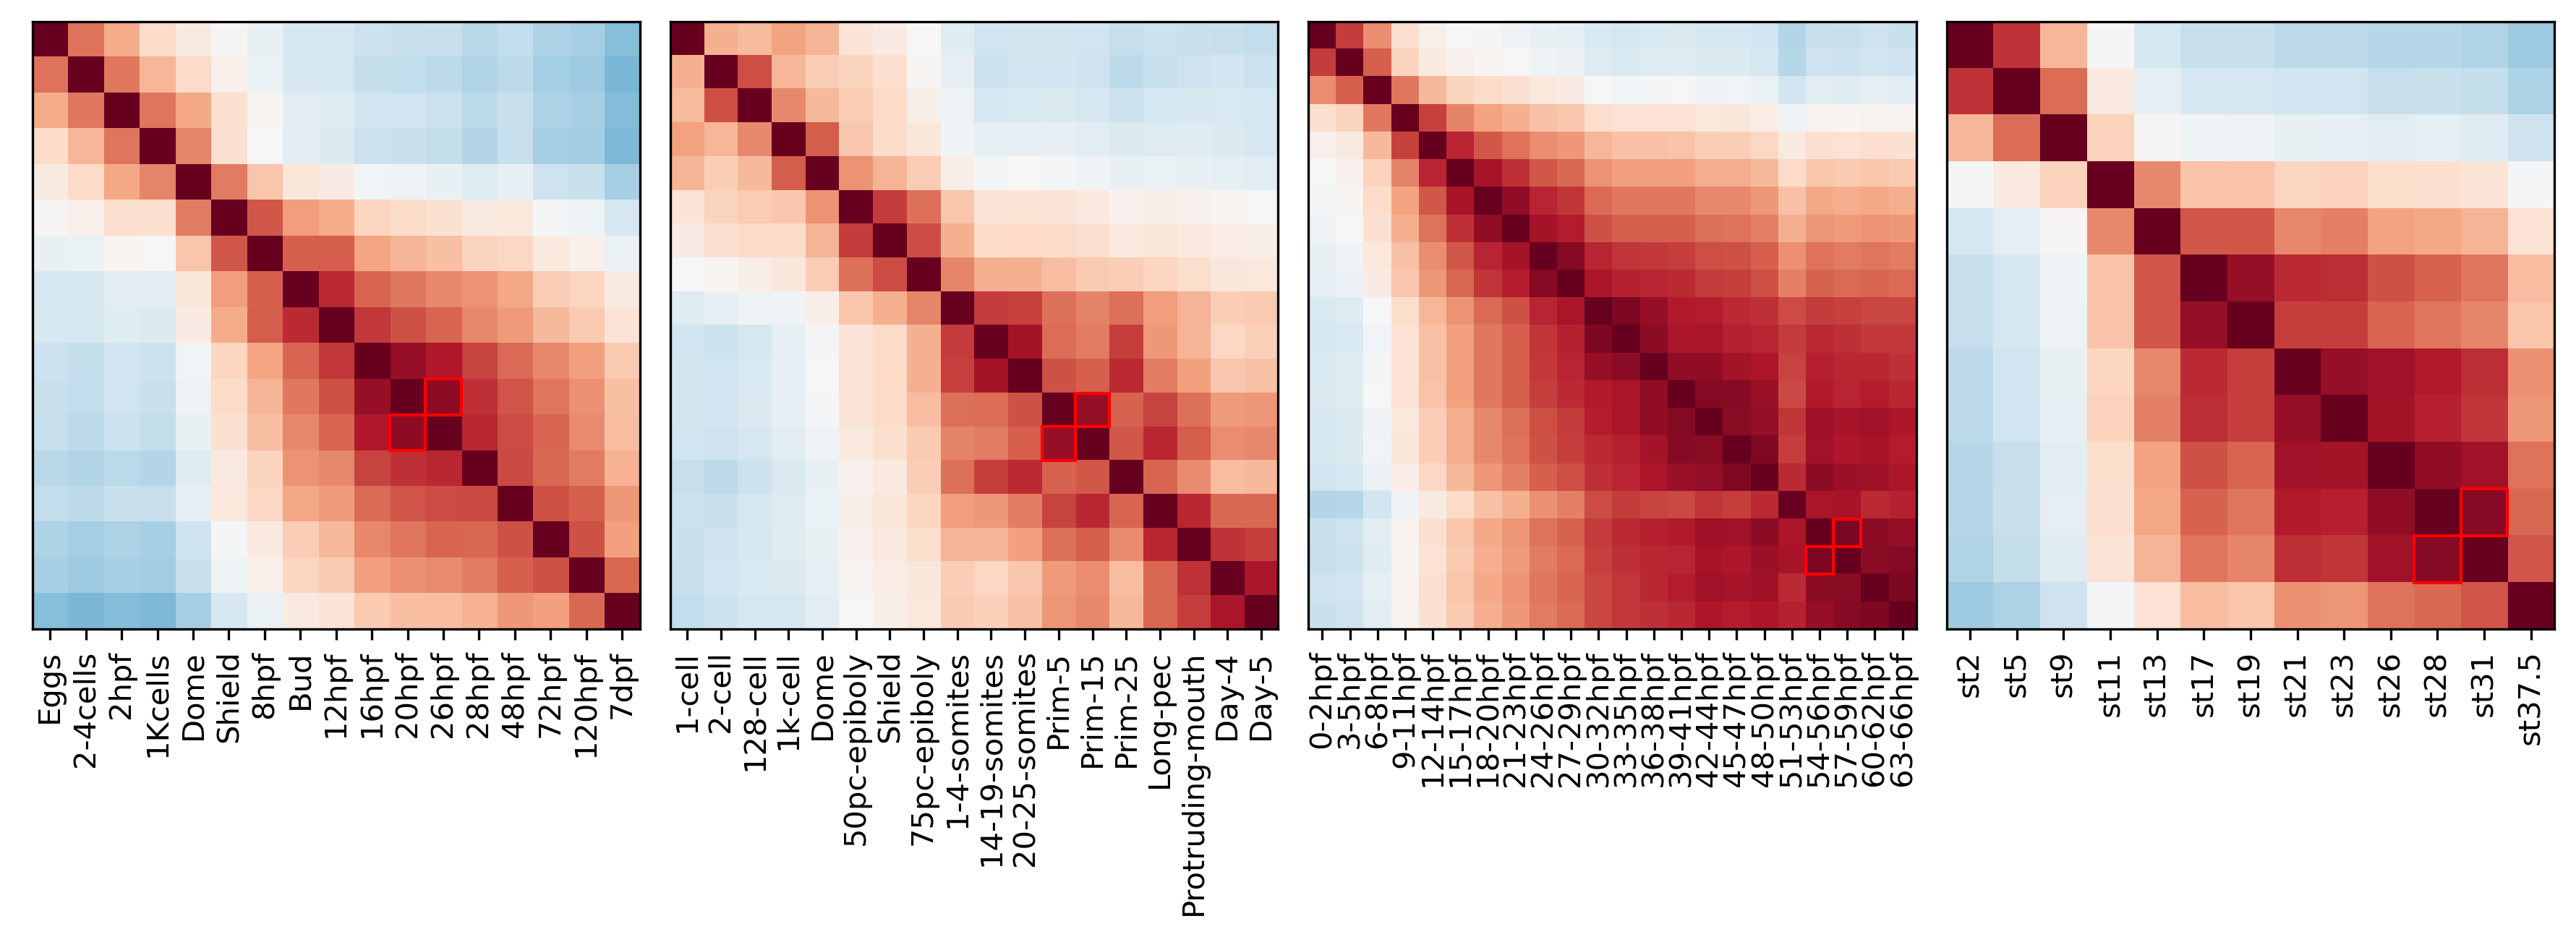
\includegraphics[width=\linewidth]{ch.hourglass/images/within_species.png}
    \caption{Self-correlation of different}
    \label{fig:withinspecies}
\end{figure}

\begin{figure}[H]
    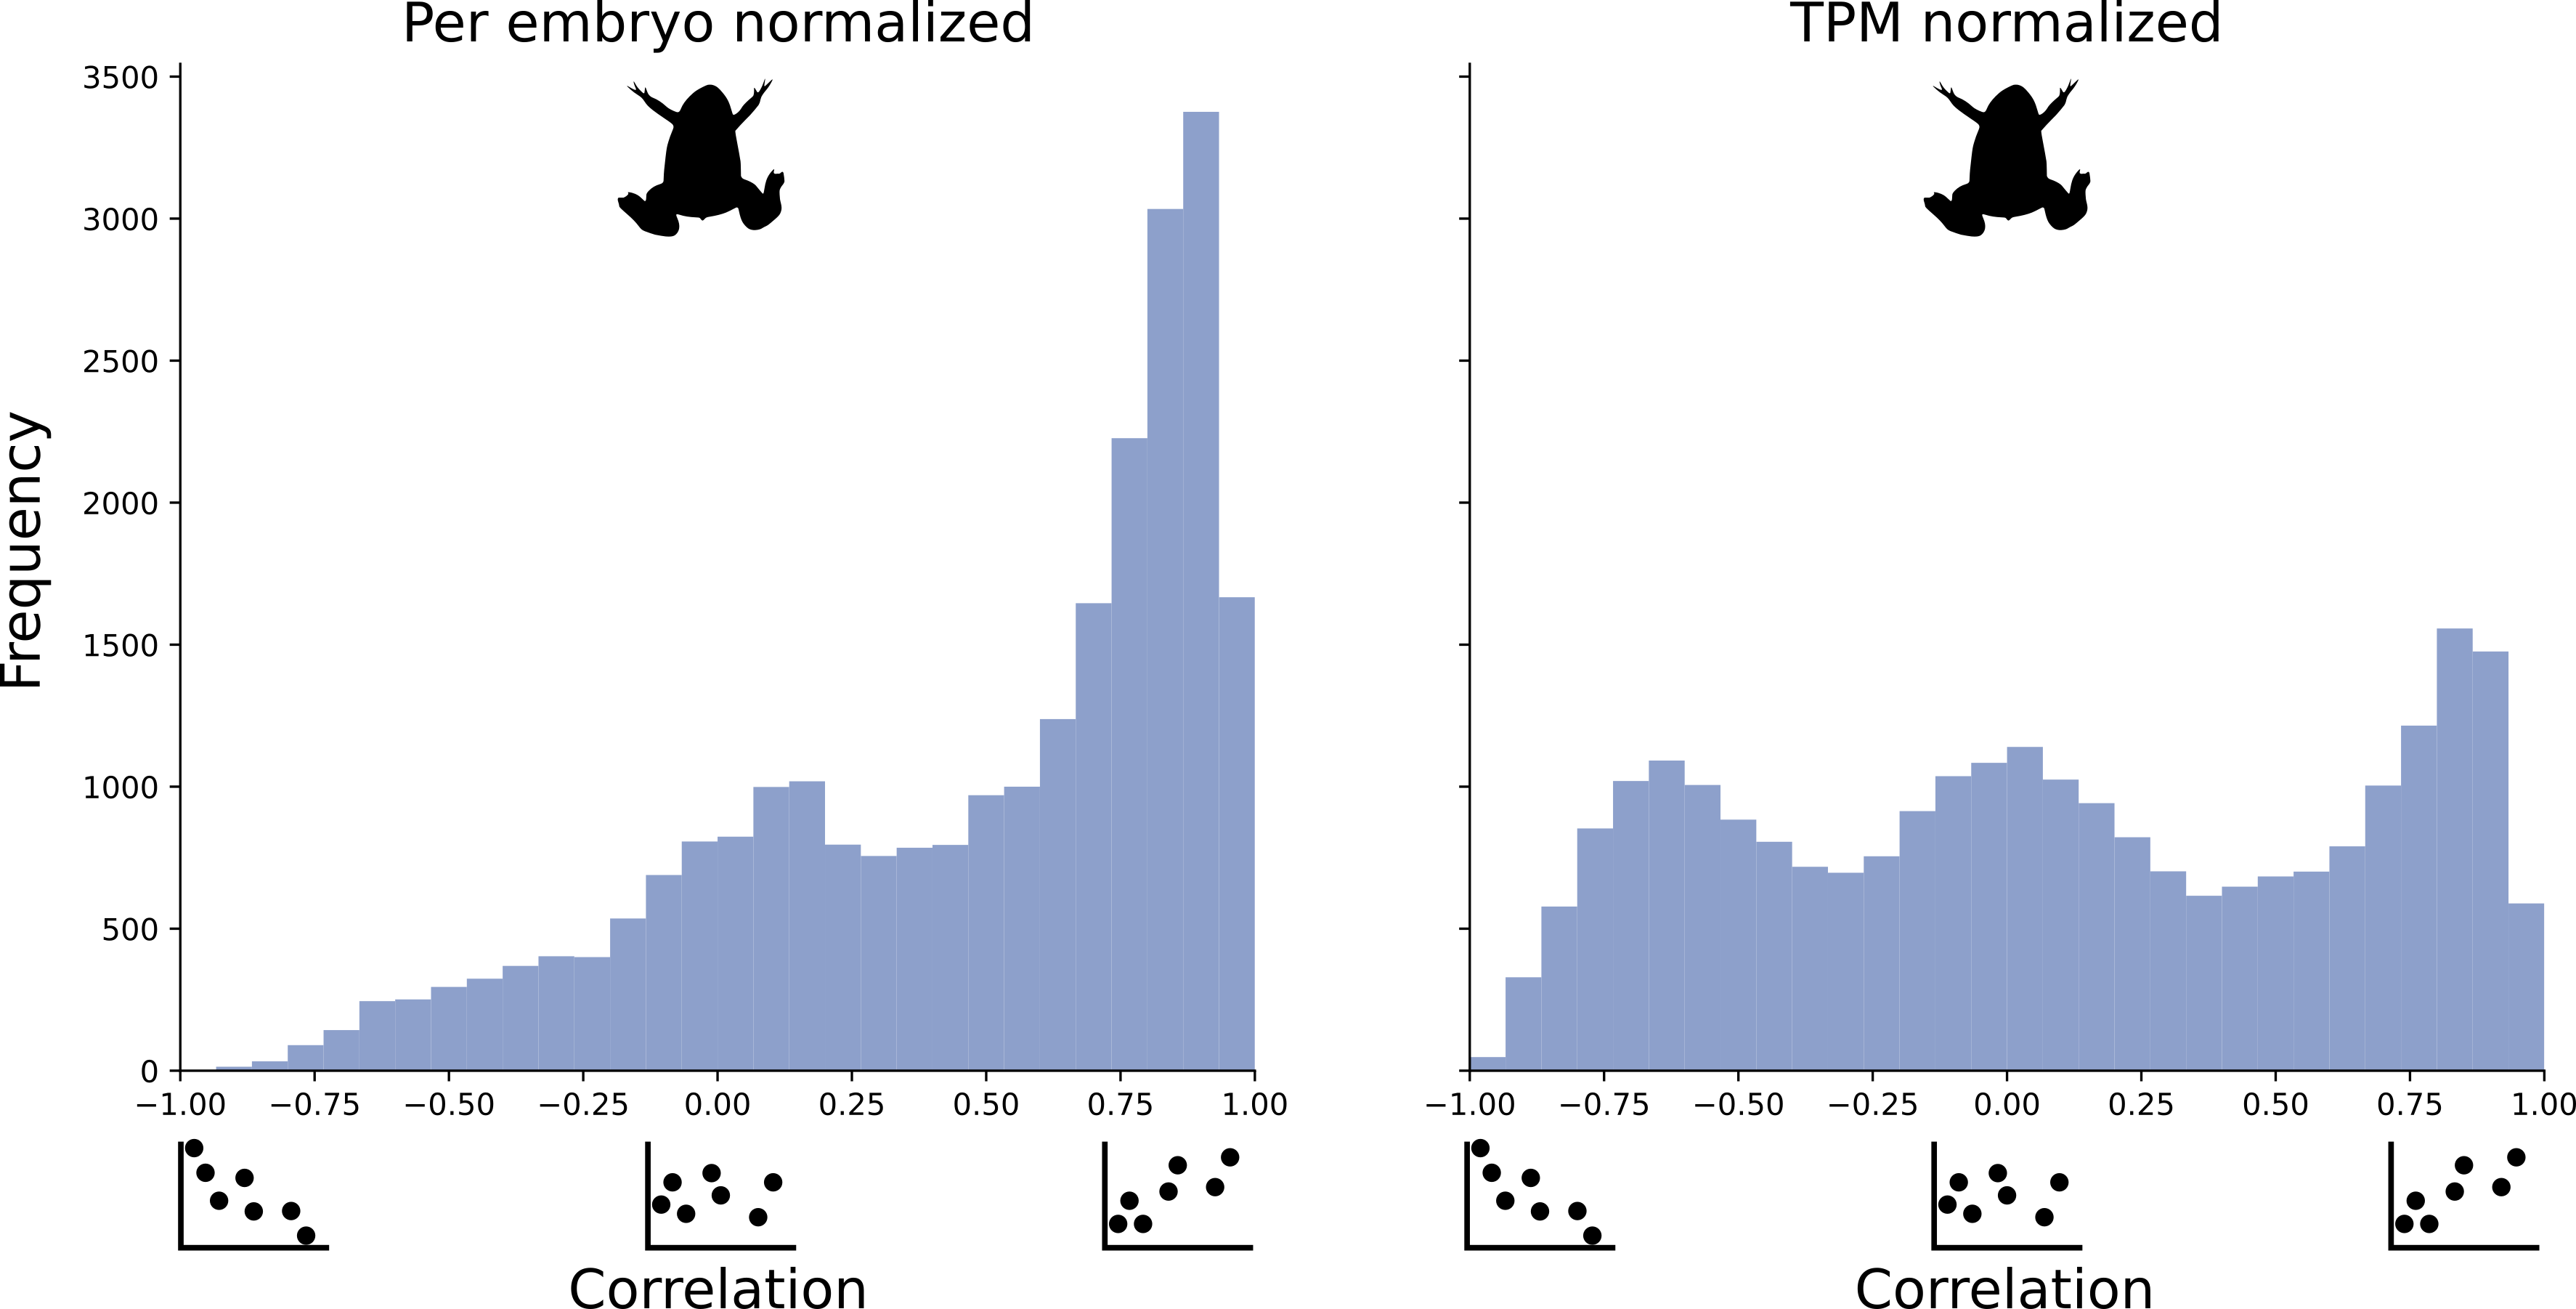
\includegraphics[width=\linewidth]{ch.hourglass/images/gene_landscape_normalization.png}
    \caption{\textbf{The global per-embryo and TPM normalized gene expression patterns are vastly different for developing \textit{X. tropicalis} embryos.} Histograms of gene landscapes between per-embryo normalization and TPM normalization of \textit{X. tropicalis}. The left panel shows the gene landscape of per-embryo normalized gene expression. Because the \textit{X. tropicalis} embryo grows in size practically all genes are upregulated considered on a per-embryo level. In the right panel the gene landscape of TPM normalized gene expression is visualized. Here we see that there are roughly three groups of gene expression, a down-regulated, a constant, and an up-regulated group.}
    \label{fig:genelandscapenormalization}
\end{figure}

\begin{figure}[H]
    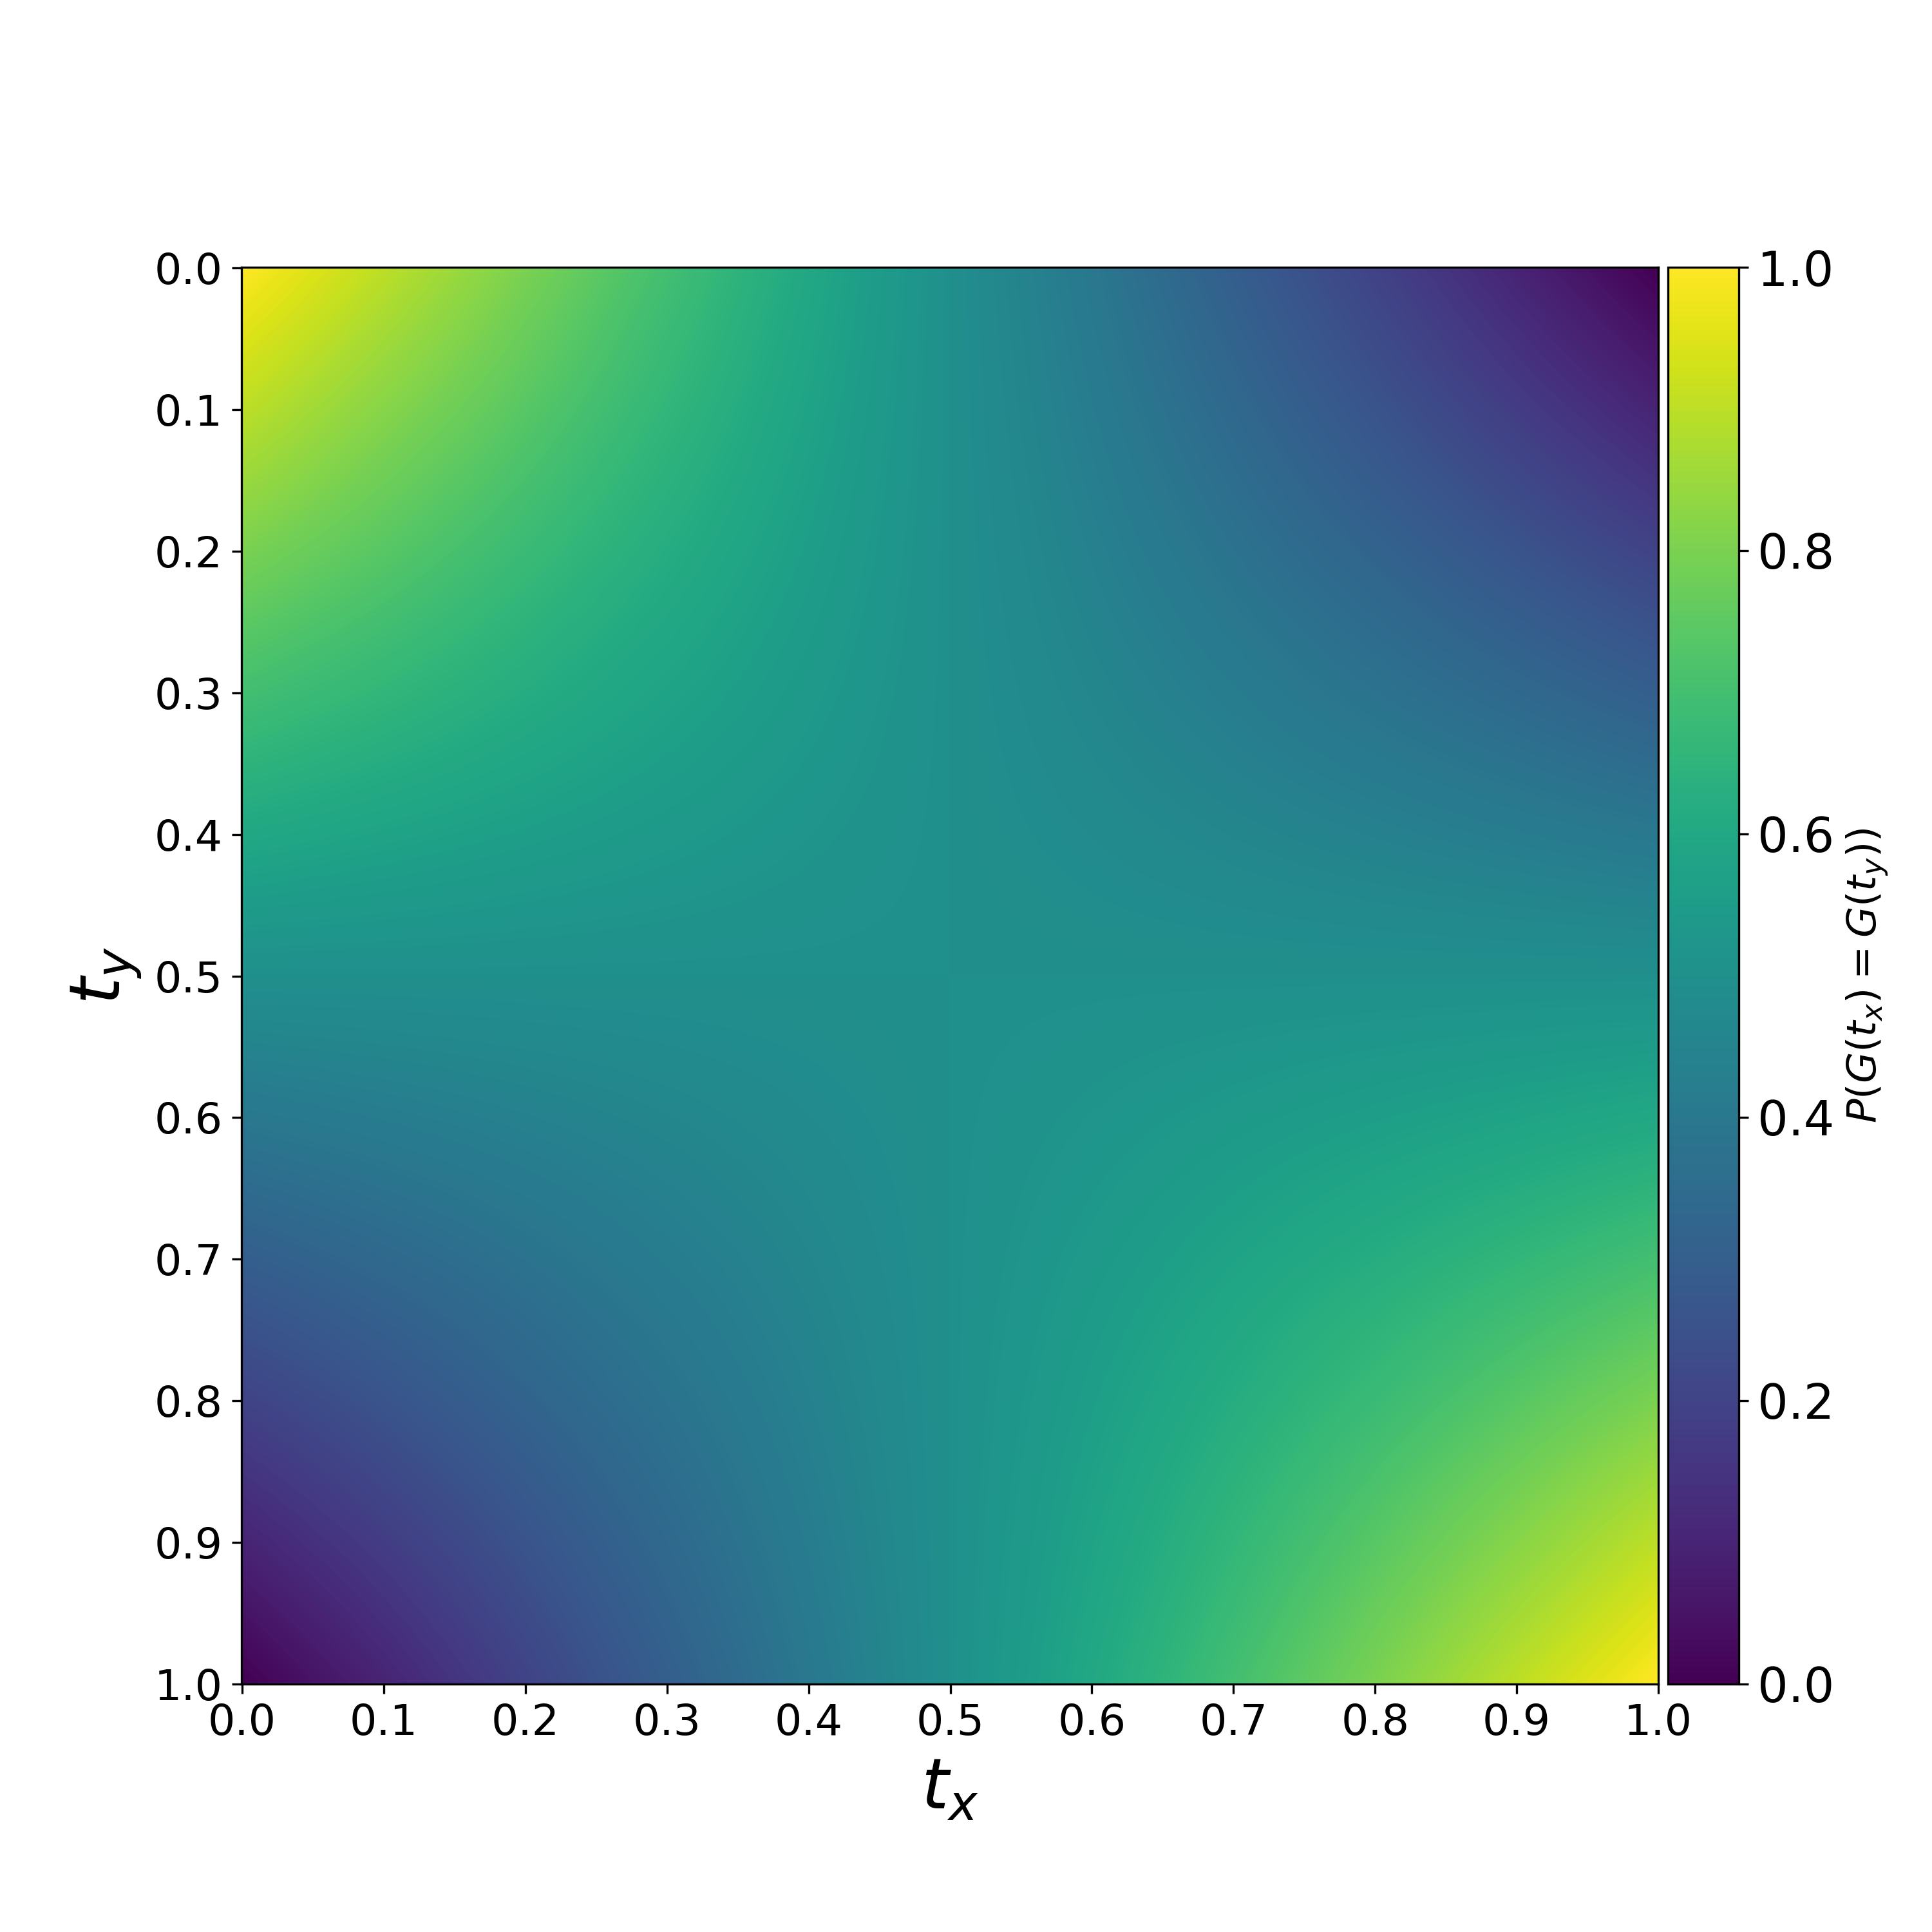
\includegraphics[width=\linewidth]{ch.hourglass/images/math_inverse.png}
    \caption{\textbf{The probability of two genes being equal in a simple system displays an inverse hourglass.} This assumes a simple system of two genes (x and y) that both start in the same \textit{off} state and at a random time point switch to an \textit{on} state. }\label{fig:inverse_math}
\end{figure}

\begin{figure}[H]
    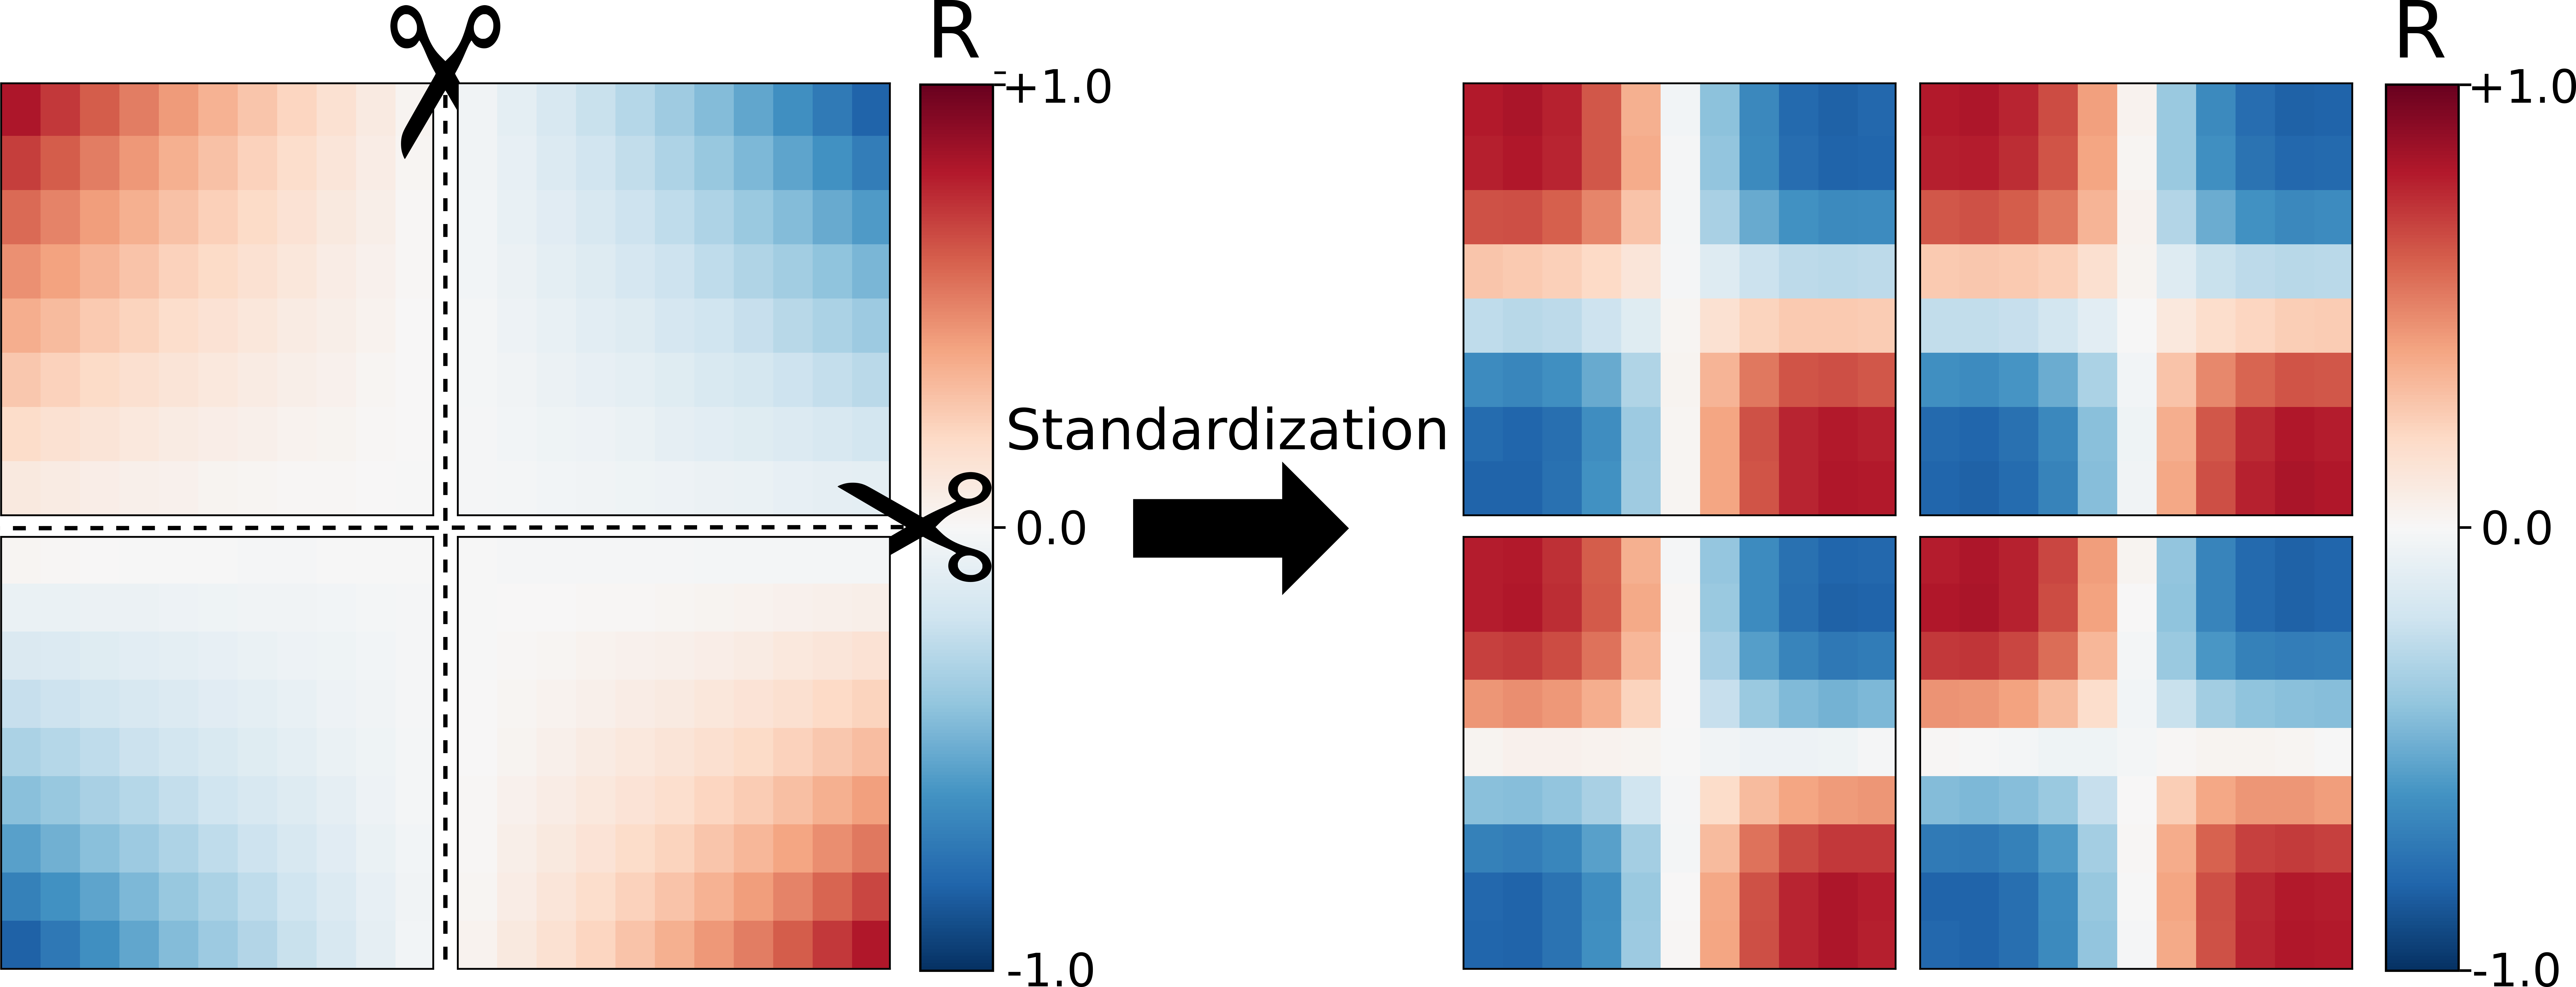
\includegraphics[width=\linewidth]{ch.hourglass/images/sim_normalisation.png}
    \caption{\textbf{Simulated data after divided into four equal parts still shows an inverse hourglass after standardization.} This is a clear indication that the simulated suffers from the same statistical artefact as the real biological data. This means that two data sets that have no temporal relation can still show a temporal pattern.}
    \label{fig:sim_normalisation}
\end{figure}

\begin{figure}[H]
    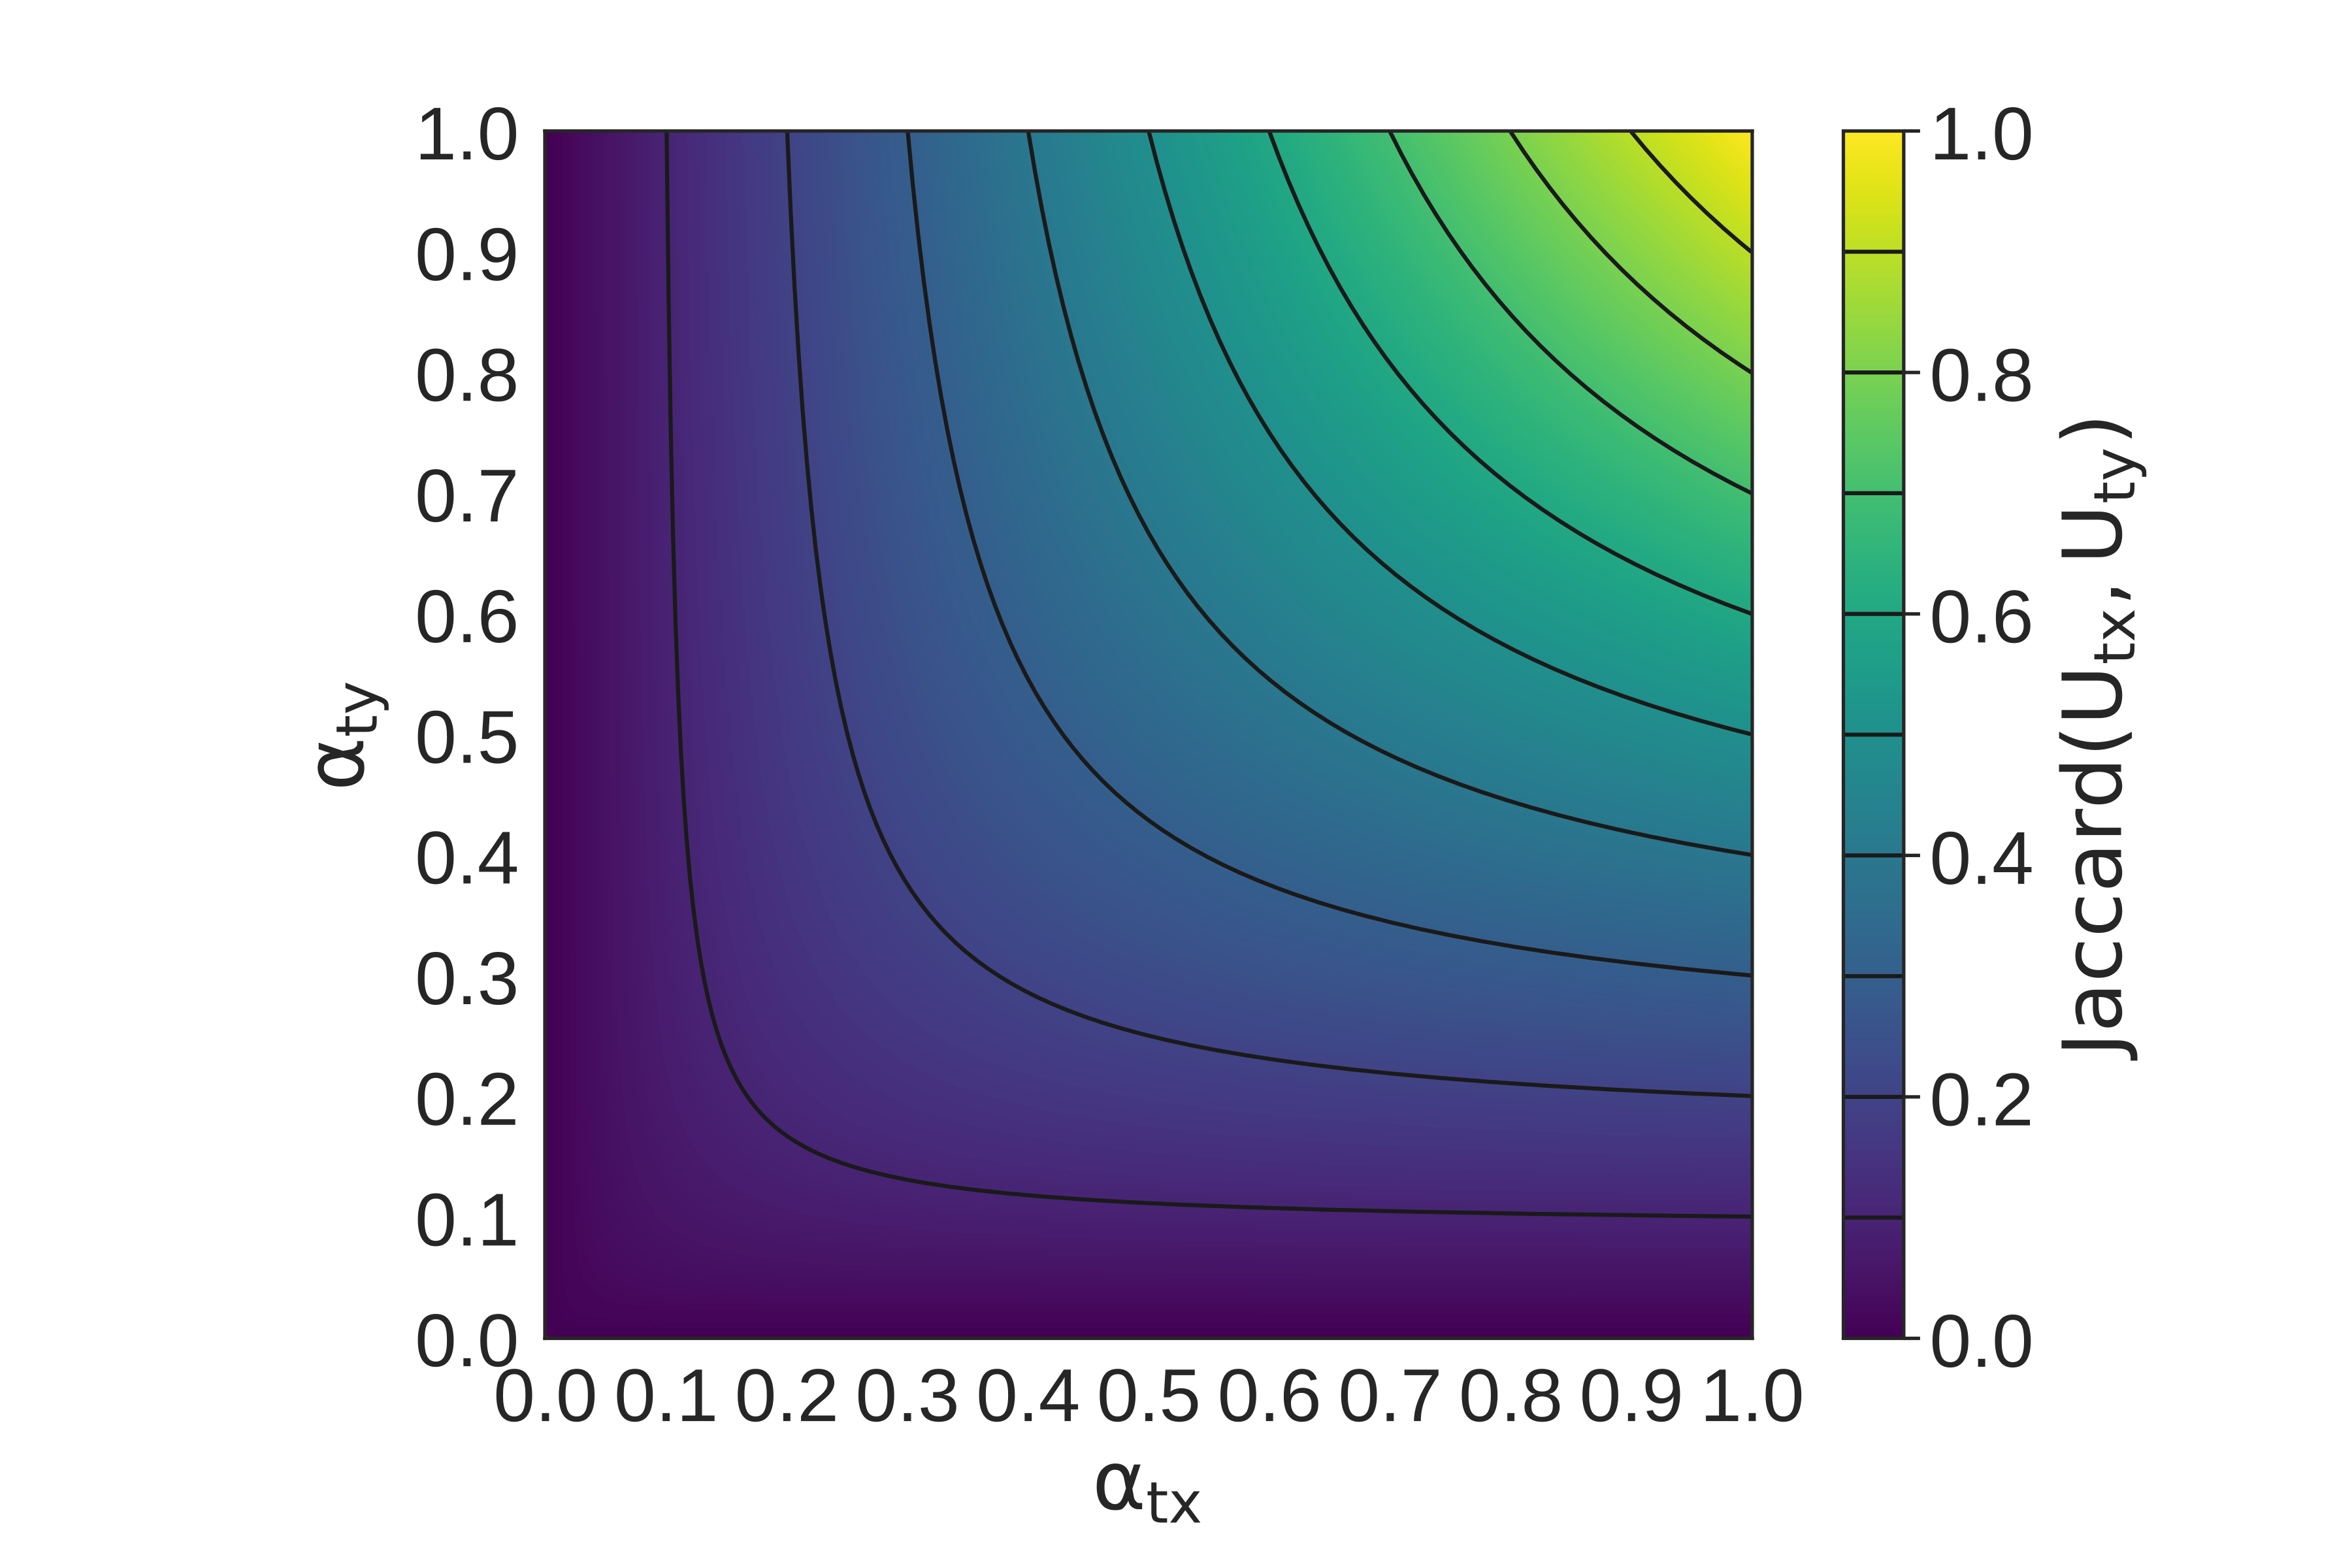
\includegraphics[width=\linewidth]{ch.hourglass/images/math_flies.png}
    \caption{\textbf{The Jaccard index landscape for a different ratio of time-point specific enhancers.} This assumes that all enhancers are shared between two species, and $\alpha_{tx}$ is the ratio of total enhancers found at timepoint $t$ for species $x$. The Jaccard index depends on the number of enhancers found, and is especially sensitive to the lowest number of enhancers found in the two time series. This effect is visible in the real data of figure \ref{fig:peak_null}D. }
    \label{fig:peak_math}
\end{figure}

\begin{figure}[H]
    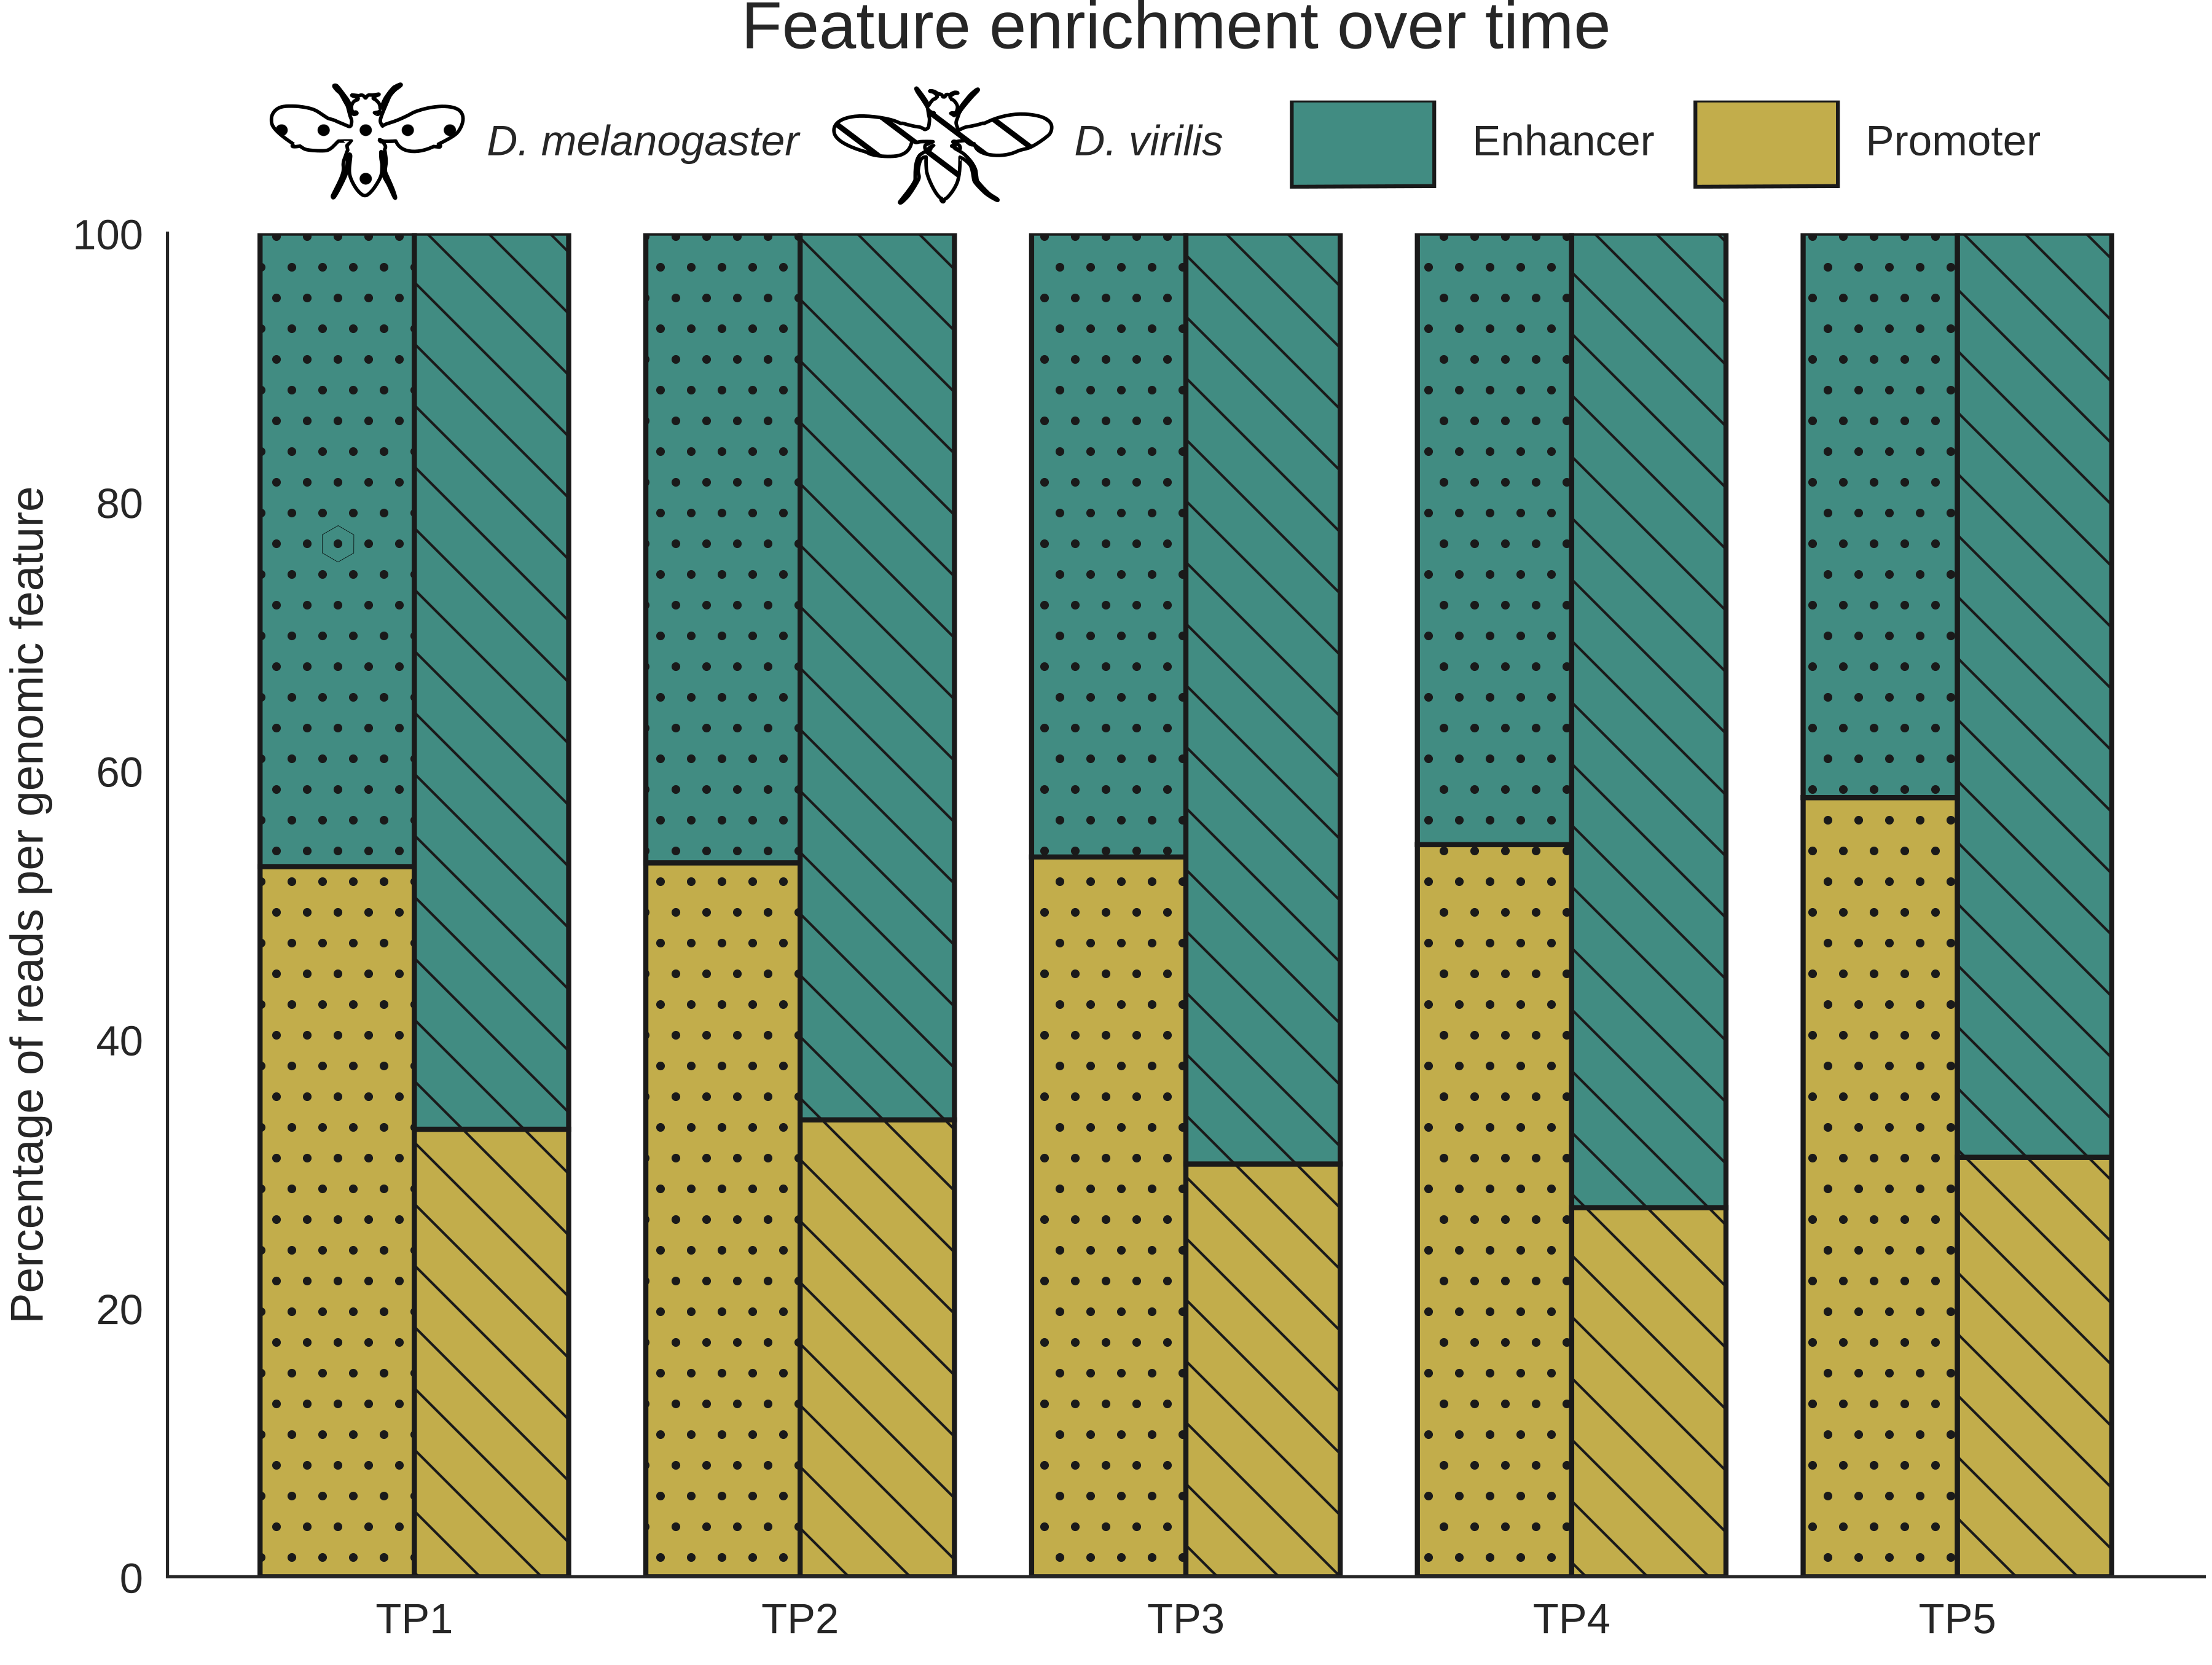
\includegraphics[width=\linewidth]{ch.hourglass/images/feature_enrichment.png}
    \caption{\textbf{There are no major sudden changes in the amount of reads}.}
    \label{fig:peak_enrichment}
\end{figure}

\closesupplement

% \chapter{Single-Cell EPigenome-based Inference of Activity}\thumbforchapter
\chapterauthor{Rebecca R. Snabel*, Maarten van der Sande*, Gert Jan Veenstra, Simon J. van Heeringen}
\newpage

\section{Abstract}

Single-cell RNA-seq (scRNA-seq) has proven to be a powerful tool for understanding gene expression profiles and cellular heterogeneity. However, as the quality of inferred gene regulatory network (GRN) from transcriptomic data is low, the need for more layers of information is required. Chromatin context, such as DNA accessibility and chemical modifications like H3K27ac, which are often enriched at cis-regulatory regions, improves GRN inference. Here we present SCEPIA, a computational tool that integrates scRNA-seq with a reference collection of (bulk) H3K27ac. We show that transcriptomic samples can be reliably and automatically matched to genomic samples. Moreover, by matching scRNA-seq with H3K27ac we improve the inferred transcription factor motif activities. Finally, we demonstrate the usefulness of SCEPIA on \textbf{HHCA TODO}. SCEPIA is available at \url{https://github.com/vanheeringen-lab/scepia.}

\section{Introduction}

The state of a cell's gene activity is shaped by a complex network of interacting genes, with a special role reserved for transcription factors (TFs). TFs bind to cis-regulatory DNA and change its chromatin state or interact with other transcription factors in proximity\cite{Spitz2012}. This in turn regulates the rate of transcription of the related genes. As such, to understand transcription regulation it is crucial to have an understanding of the interplay between cis-regulatory regions and transcription factors. To this end, genomic assays such as histone- and transcription factor ChIP-seq\cite{Robertson_2007}, DNAse-seq\cite{Boyle_2008}, and ATAC-seq\cite{Buenrostro_2013} have been developed. These assays allow for the precise measurement of histone modifications, transcription factor binding, and DNA accessibility, and consequently for the inference of cis-regulatory elements and their related TFs.

Single-cell transcriptomics has emerged as a rapidly expanding field, allowing researchers to explore the gene expression profiles of diverse cell types with increasing ease and affordability. However, when it comes to examining DNA accessibility, transcription factor binding, and histone context, crucial aspects of transcription regulation, challenges persist. Single-cell ATAC-seq (scATAC)\cite{Buenrostro2015_sc}, while immensely valuable, remains costly and generates sparser data compared to single-cell transcriptomics and bulk genomic methods\cite{Li2021}. Similarly, single-cell CUT\&Tag (scCUT\&Tag)\cite{Bartosovic2021}, a method able to measure histone modifications as well as transcription factor occupancy on a single-cell level, \textbf{something about difficult and expensive}. Consequently, many laboratories encounter difficulties in adopting these techniques.

As genomic information is crucial for understanding gene regulation, but remains hard to acquire in single-cell data, linking single-cell transcriptomic data to bulk reference genomic databases is a standard practice. For instance, the computational tool SCENIC infers transcription factor co-expression regulons based on single-cell transcriptomic data, and refines these regulons based on the presence of relevant motifs in cis-regulatory regions surrounding the genes within a reference genomic database\cite{Aibar_2017,VandeSande2020}. Similarly, the computational tool SCRIP combines single-cell ATAC-seq with a reference database to get a blended bulk and single-cell per-gene signal. This approach mitigates the downsides of single-cell ATAC-seq, which is noisy and sparse, but still profits from its resolution\cite{Dong2022}. These tools show a successful integration of single-cell data with a reference database. And given that the information in genomic assays and transcriptomic assays is partially redundant\cite{Wang2016,GonzlezRamrez2021}, the opportunity arises for automatically associating transcriptomic data with genomic assays of a similar cell type. Furthermore, the combination of both genomic and transcriptomic data has been shown to enhance the inference of gene regulatory networks\cite{Xu_2020,Kamal_2021}. This poses an intriguing concept: automatically linking single-cell transcriptomic data to a bulk genomic reference, which in turn potentially improves transcription factor motif activity inference.

Here we explore the question of whether (single-cell) transcriptomic data can be linked to a genomic reference collection to improve transcription factor motif activity inference. This approach has two advantages. First, single-cell RNA-seq is cheaper and easier to perform than single-cell genomic assays (scATAC, scCut and Tag). Moreover, by automatically linking single-cells to a genomic reference one gets multiome data. Second, by using the reference data for motif activity inference it is possible to compare gene expression and motif acvitiy, and remove spurious interactions. We call this approach Single-cell EPigenome-based Inference of Activity (SCEPIA). We test on HHCA..

% This reference database can be used for motif scanning.  To \textit{test} how SCEPIA performs on real data, we have used the latest version of the human Heart Cell Atlas v2 (REF XXX HHCA v1, HHCA v2). The version 2 of this dataset additionally consists of single-cell chromatin accessibility data alongside transcriptomic data from the same nuclei, by combining both versions of the atlas the authors produced an extensive atlas covering the different tissues and cellular subtypes present in the human adult heart. A lot is known about different cellular markers and regulators of the different cell types within the heart, however, much can also still be gained from more detailed research on further epigenetic regulation within the heart, and the transcriptional actors contributing to this. However, in this research only the openness of the chromatin is captured, not the more detailed information on the histone modification differences, which can inform on whether an accessible region acts as an active enhancer. Cardio-vascular diseases are still the number one cause of deaths worldwide (\href{https://doi.org/10.1161/CIR.0000000000001123}{https://doi.org/10.1161/CIR.0000000000001123}), and the ability to research intricate differences between healthy and diseased tissues in a multimodal setting, will help to gain more understanding of the complex (dis)regulation happening in these tissues, also on the less researched field of epigenetic on a cellular//cell type level. 

% The availability of the single-cell chromatin accessibility data, can be used as an epigentic read-out and thereby brings us one step closer to the type of data SCEPIA will infer. This allows us to validate the performance of our tool in predicting epigenetic/transcriptional regulation from a single-cell transcriptomic dataset. // SCEPIA infers per single cell the active enhancer signal from public ChIP-seq data resources, although accessibility of the chromatin is one read-out of the effect of such active enhancer signal.

\section{Results}

\subsection{Matching Regulatory Potential and Transcripts Per Million}

We hypothesized that incorporating a measure of cis-regulatory element activity, such as ATAC-seq or H3K27ac ChIP-seq, would be beneficial to identify transcription factor motif activity from single-cell transcriptomic data, even when this is not experimentally measured. Here, we used the \textit{regulatory potential} to match single-cell RNA-seq profiles to a collection of known H3K27ac ChIP-seq profiles. The regulatory potential is defined as the weighted average H3K27ac signal per gene \cite{Wang2016}. To determine how well regulatory potential specifically matches RNA-seq data for identical (or similar) cell types, we obtained data from 96 human RNA-seq cell types and 121 human H3K27ac cell types from ENCODE\cite{encode_dcc} (Supplementary \textbf{Table SX}). We calculated the regulatory potential for all H3K27ac samples (see Methods). We then computed the correlation coefficient for all possible combinations of regulatory potential and RNA-seq values (Fig. \ref{fig:bulk_comparison}). In general, the regulatory potential shows only a high positive correlation for a subset of the transcriptomic data, indicating that the measure captures a cell type-specific signal. The mean correlation coefficient for identical cell types between regulatory potential and transcripts per million (TPM) was found to be 0.53 with a standard deviation of 0.14. In 64\% of instances, the regulatory potential of a given cell type exhibited the highest correlation with the TPM of the same cell type. Furthermore, in 77\% of the cases, the highest correlation was observed with a tissue sharing the same ontology term. As noted previously \cite{Wang2016}, the specific parameters used for calculating regulatory potential do not significantly impact the results. For this specific analysis, the H3K27ac signal in the promoter region alone is sufficient to predict the TPM (table \ref{table:correlations}). In summary, our findings suggest that a collection of H3K27ac regulatory potential can effectively serve as a reliable classifier for characterizing cell states based on transcriptomic data.

\begin{figure}
    \centering
    \includegraphics[width=1\linewidth]{ch.scepia/imgs/celltypes.png}
    \caption{\textbf{Transcriptomic counts are a reliable predictor for H3K72ac cell state and automatically matching assays improves motif activity inference.} \textbf{(A)}: The Pearson correlation coefficients between all combinations of 121 H3K27ac regulatory potentials and 96 RNA TPMs. In 77\% of the comparisons, the highest correlation between TPM and regulatory potential was observed between samples with the same ontology term. \textbf{(B)}: Motif activities based on samples automatically matched to a reference H3K27ac collection are more accurate than on transcriptomic data alone. The motif activities between 5 random cell types are inferred based on their H3K27ac signal in their top 25,000 differential enhancers (100 permutations). The naive approach to motif activity inference with only transcriptomic data is to assume that the TPMs of transcription factors are directly related to their motif activity. The naively inferred motif scores only have an average correlation score of 0.04 with the true motif scores. The regulatory potential-based approach automatically matches a transcriptomic sample to an H3K27ac sample and infers the motif activity scores on their top 10,000 differential enhancers (\textbf{mean of XX}). The identical sample in the H3K27ac reference database \textbf{is held out}. Finally, as the motif activities are based on the top 25,000 differential enhancers, the subset models the correlations between motif activities on the top 10,000 and top 25,000 differential enhancers (\textbf{mean of XX}).}
    \label{fig:bulk_comparison}
\end{figure}

In general, the H3K27ac signal in regulatory sequences can be used to determine motif or transcription factor activity\cite{FANTOM2009,Balwierz2014,Madsen_2017}. This motif activity, which quantifies the contribution of each motif to H3K27ac peak strength, has been shown to be a powerful measure of the relevance of a transcription factor for a specific cell state. The relationship between RNA-seq and regulatory potential led us to assume that transcription factor motif activity can be inferred from transcriptomic data, through an intermediate collection of matched H3K27ac data. As the reference collection contains a limited number of cell types, an exact matching cell type may not always be available for a specific cell type measured by RNA-seq. Therefore, we decided to calculate a composite measure of motif activity, based on a combination of reference cell types. To calculate this measure, we regressed the TPM values of the 2,000 most variable genes of a collection of cell types against our regulatory potential database. From there, we selected the top 50 cell types based on the absolute regression coefficients and identified the top 10,000 most differentially enriched cis-regulatory regions within these 50 cell types. Subsequently, we calculated the motif activity using these enhancers, and obtained the final motif scores by taking the dot product of motif scores and regression coefficients. 

To test our composite activity score, we made one hundred random subsets of five tissues common to both our H3K27ac reference database and transcriptomic dataset. Our first step involved establishing a ground truth for motif activities by conducting a motif scan on the top 25,000 most differentially enriched enhancers within each of these five tissues. Here, enhancers were defined as peaks within the REMAP dataset located more than 2kb away from the transcription start site. A naive approach to estimating motif activity based solely on transcriptomic data would assume a direct one-to-one translation between the transcripts per million (TPM) values of a transcription factor and its motif score. However, as Figure \ref{fig:bulk_comparison}B illustrates, this naive approach displays a particularly poor correlation with our ground truth data. Instead, our approach based on regulatory potential demonstrates a significantly improved correlation compared to the naive method (Figure \ref{fig:bulk_comparison}B). Note that the cell types used for the ground truth are excluded from the reference database. Finally, to assess the sensitivity of our approach to the choice of enhancer set, we compared the ground truth data based on the top 25,000 most variable enhancers with that based on the top 10,000 most variable enhancers. Taken together, these analyses show that RNA-seq can be reliably matched to H3K27ac in a cell type-specific manner and that this data can be used to estimate transcription factor activity. See supplemental \textbf{figure XXX, still to come} for parameter sweep, that shows ??. 

\subsection{Single-Cell EPigenome-based Inference of Activity}

The previous section demonstrates the reliable matching of gene counts to an H3K27ac reference using regulatory potential. This matching process enhances the inference of transcription factor motif activity, even in the case where the exact matching cell type is absent in the reference. Given the ability of single-cell sequencing to finely separate between cell types, this methodology can be effectively extended to single-cell RNA-seq. Additionally, the increased number of measurements in single-cell sequencing facilitates more sophisticated significance testing, further strengthening the analytical capabilities of the method (\textbf{this is a bit sketchy though..}).

\begin{figure}
    \centering
    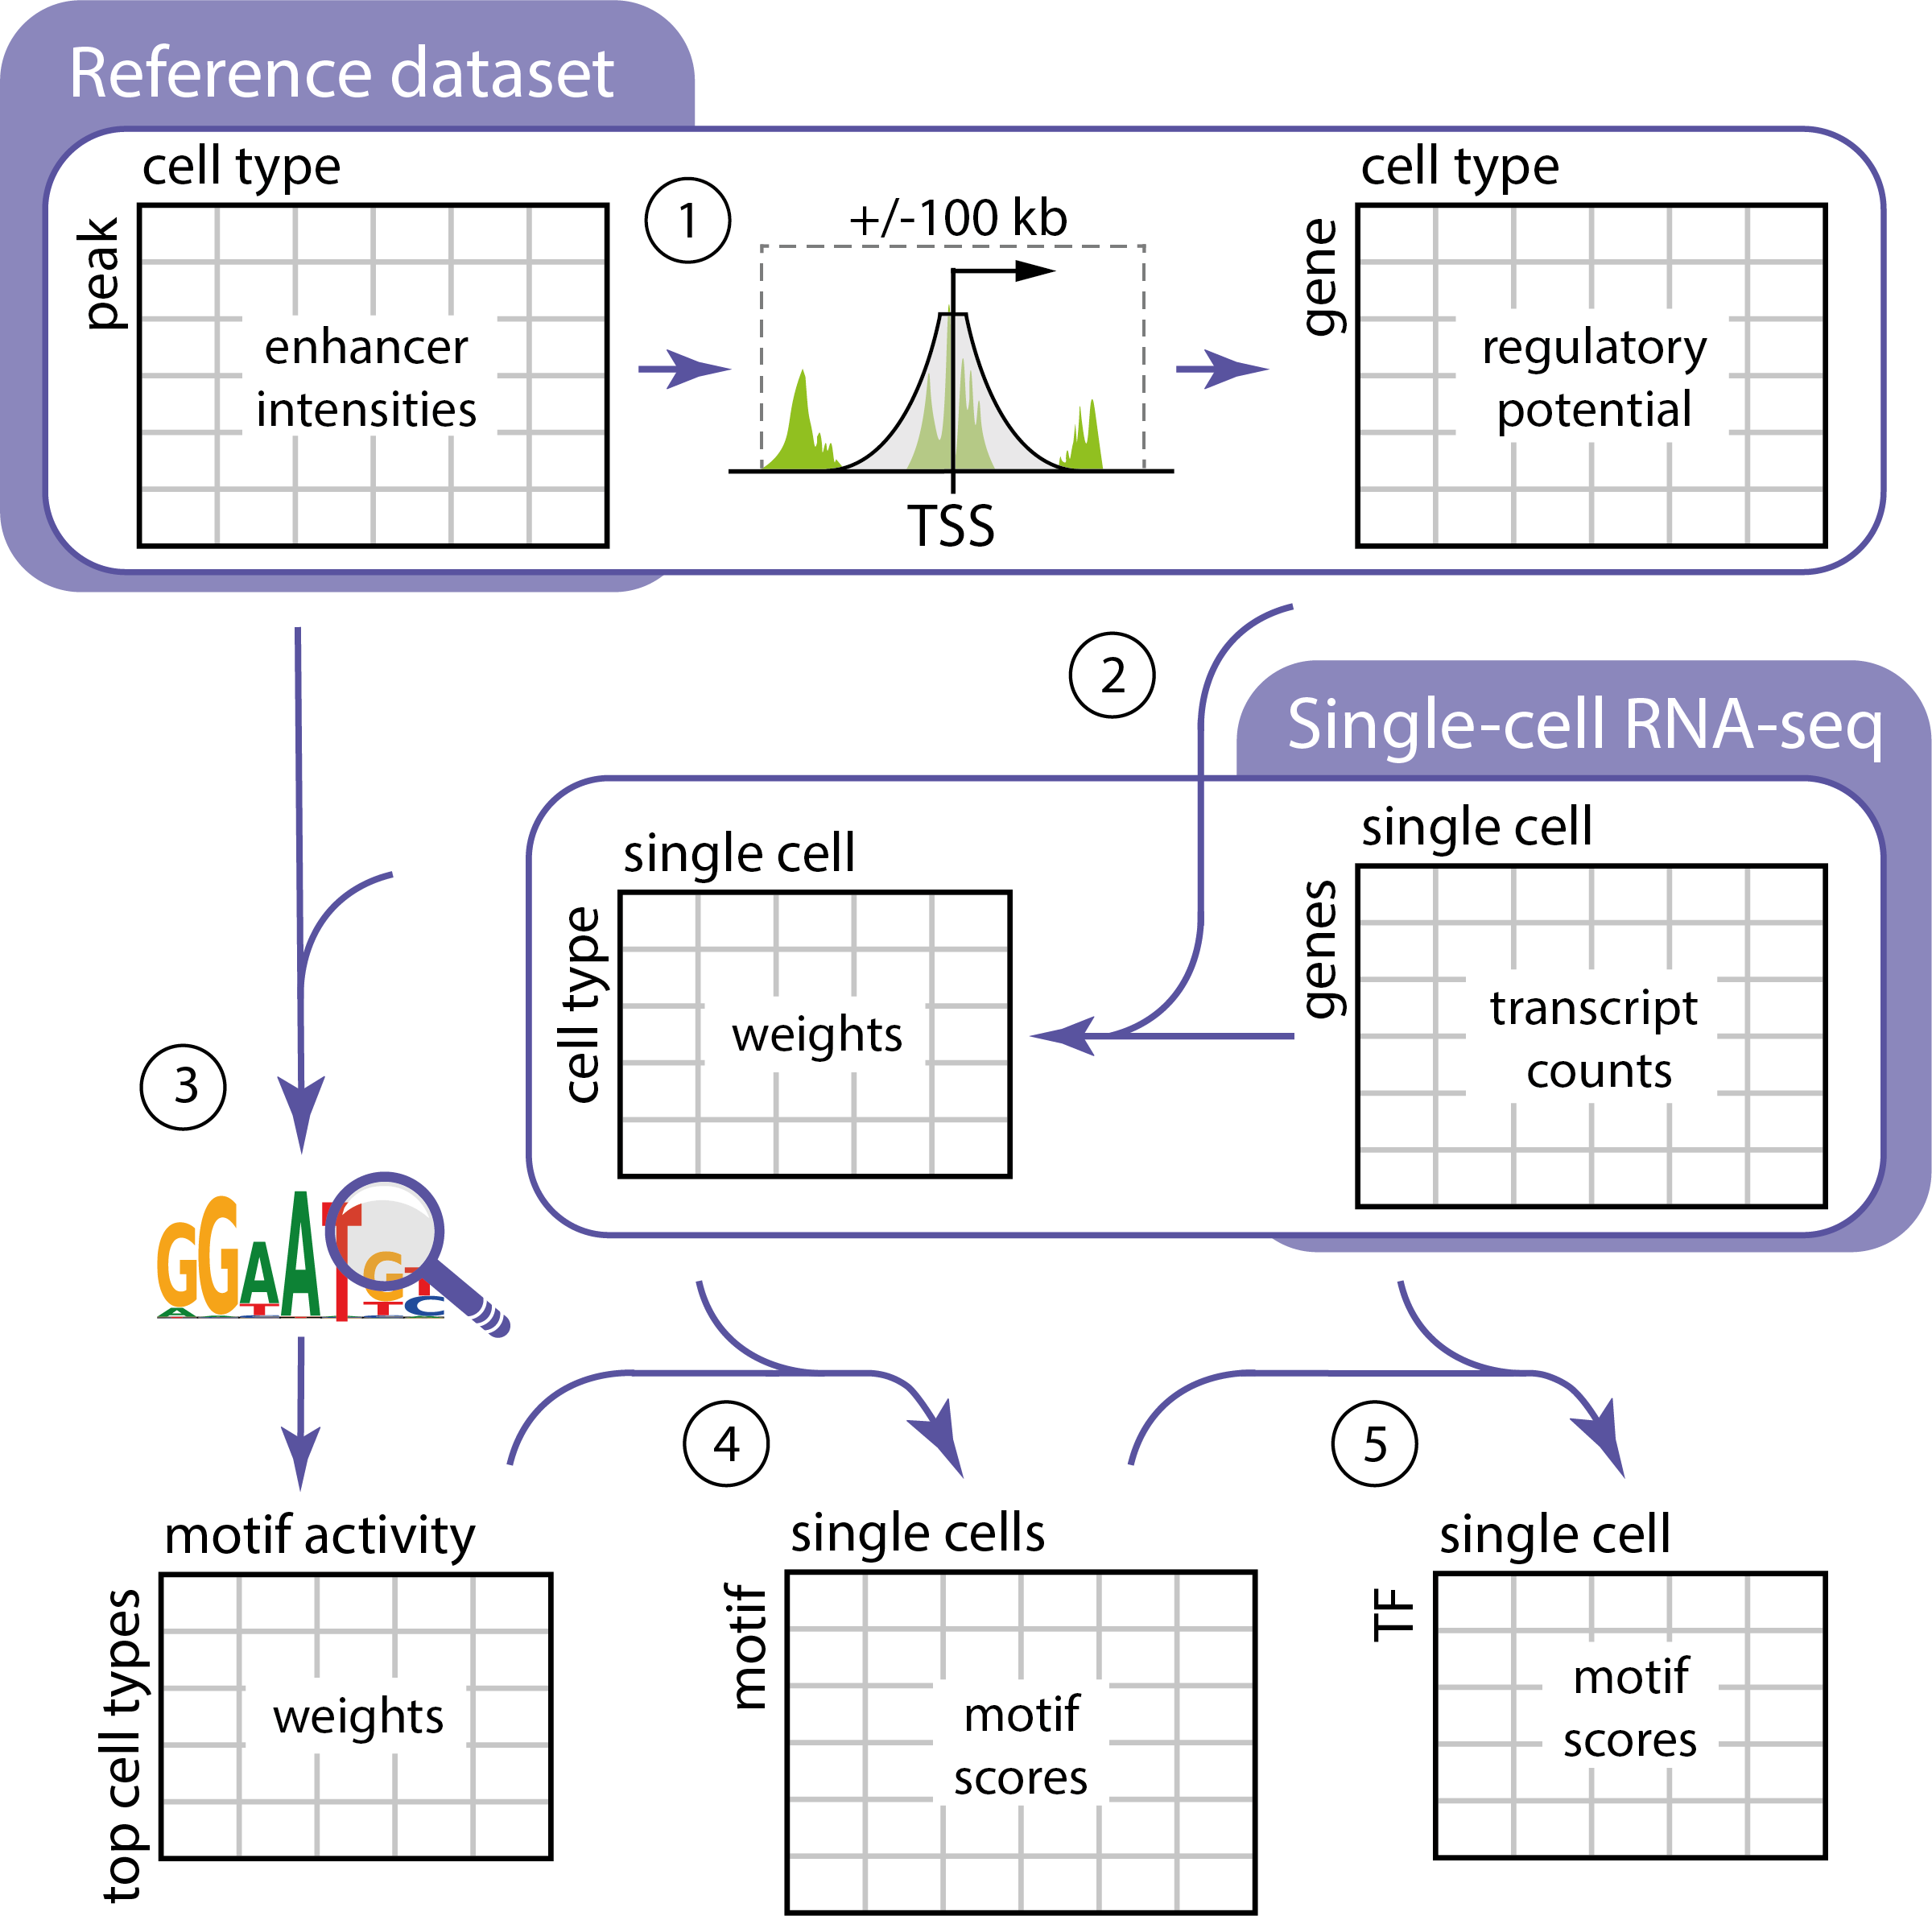
\includegraphics[width=1\linewidth]{ch.scepia/imgs/20231106_OverviewFigure_SvH_v2.png}
    \caption{\textbf{Schematic overview of Single-Cell EPigenome-based Inference of  Activity (SCEPIA).} See the methods for an extensive explanation per step. \newline 
    \textbf{Step 1}: Calculate the regulatory potential from distance-weighted chromatin-assay intensities around each gene for each cell type in the reference collection.
    \textbf{Step 2}: Regress the single-cell gene expression on the regulatory potential. Keep the top 50 cell types with the absolute highest regression coefficients, and use those as the cell type weights for each cell.
    \textbf{Step 3}: Select the top 10,000 most differential \textbf{peaks/enhancers/...} between the top 50 cell types, and use them for motif activity inference.
    \textbf{Step 4}: Take the dot product between the motif activities and the cell type weights, resulting in motif activities for each motif per cell. Motif activities are scaled to a motif score between 0-1. 
    \textbf{Step 5}: Calculate the correlation coefficient between all pairs of TF gene expression and motif activities. A permutation test between gene expression and motif activities allows for the estimation of the statistical significance of their relation.}
    \label{fig:scepia_overview}
\end{figure}

To test SCEPIA on a scRNA-seq data source for which matching single-cell chromatin accessibility data was available, we used the human Heart Cell Atlas v2 (hHCA) multiome data (\cite{Kanemaru2023}). Since SCEPIA performs motif activity inference solely informed on the scRNA-seq data, we evaluate how this compares to motif activities found in the actual accessible chromatin of these cells. Furthermore, SCEPIA selects regulatory factors based on motif activity combined with the TF's expression levels and we validate how this compares to a selection based on motif activity alone. // we validate if SCEPIA's selection of regulatory factors based on expression of the TF as well as its predicted binding motif activity, improves the selection based on motif activity alone.

To confirm that matching cell types \textcolor{red}{on inferred transcriptomes} also works for a single-cell source, we compared the inferred annotation by SCEPIA with the cluster annotation as profided by the authors. // First, we ran SCEPIA on the whole hHCA scRNA-seq dataset and compared the inferred annotation with the cluster annotation as provided by the authors. SCEPIA correctly assigned the atrial and ventricular cardiomyocyte clusters correctly to heart ventricle and cardiac atrium, respectively. The fibroblasts, neural cells and mural cells (i.e. smooth muscle cells or pericytes of the vasculature), all matched to tissue or cell types similar to their identity, albeit these originated from a different organ or tissue (i.e. lung or tibia) (Figure 3A). Also the myeloid and lymphoid clusters were matched with a cell type of the correct major immune lineage branch, namely CD14+ monocytes and CD8+ T cells, respectively. It was more difficult for SCEPIA to correctly match the endothelial cells, which showed the best match with heart left ventricle and only to a lesser degree to an endothelial cell type (Fig. \ref{fig:scepia_annotation1})\textcolor{red}{, however, the endothelial cells make up a large fraction of the heart's myocard, as can also be deduced from the cluster size within the atlas, which could explain this result. Ultimately in SCEPIA's analysis, the endothelial cluster was represented by a combined signature of left ventricle and an endothelial cell type. Likewise, the adipocytes are represented by a mixed signature of right cardiac atrium and adipose tissue (Fig \ref{fig:scepia_annotation1}).} For the mesothelial cluster, there was no matching cell or tissue type available in the ENCODE database, which could explain the lack of any strong matches for this cluster. These results highlight that SCEPIA matched the majority of the clusters to similar cell types in the ENCODE reference. 

\textcolor{red}{After the initial step of matching the single cells to the cell types of the H3K27Ac reference, we now want to determine which transcriptional regulators SCEPIA considers to be of importance in these cell clusters.} Within the top hits identified by SCEPIA, multiple known markers for cell types present in the atlas were observed (Figure 3B). \textit{FLI1}, \textit{ETS1} and \textit{KLF2} are known for their roles in immune and endothelial cells (REF XX). Other examples include the well-known cardiomyocyte regulators such as \textit{TBX5} and \textit{HEY1}, \textit{PPARG }as a regulator for adipocyte differentiation, \textit{SOX17} marked specifically the endothelial cells and RUNX1 as lymphoid marker (Figure 1C). The \textit{TBX5} predicted motif activity in the cardiomyocyte clusters follows the patterns of expression, with further increased levels in the atrial cluster specifically. The motifs identified for \textit{SOX17} and \textit{RUNX1} showed variable accessibility across and within various clusters of the atlas, although both were further enriched in the endothelial and lymphoid cluster respectively (Figure 1C). \textit{BACH2} is a known repressor and immune-regulating transcription factor and implicated in neural differentiation (\href{https://www.ncbi.nlm.nih.gov/pmc/articles/PMC8934237/}{https://www.ncbi.nlm.nih.gov/pmc/articles/PMC8934237/}, \href{https://pubmed.ncbi.nlm.nih.gov/16631738/}{https://pubmed.ncbi.nlm.nih.gov/16631738/}), and IKZF1 is described as both repressor and activator in immune cells (\href{https://www.ncbi.nlm.nih.gov/pmc/articles/PMC5865415/}{https://www.ncbi.nlm.nih.gov/pmc/articles/PMC5865415/}). The latter two were identified by SCEPIA as repressors, deduced from the anti-correlation between their mRNA levels and predicted motif activities. \textcolor{red}{BACH2 expression was highest in the neural and lymphoid cluster, whereas the predicted motif (bZIP.0003) activity in both of these clusters was decreased, compared to other clusters (myeloid and endothelial showed highest motif activity; Figure S4XX). This is indicative of a repressor function in the neural and lymphoid clusters, however, for the other clusters this indicated an activating role. BACH2 is a known repressor for myeloid lineages and in neural differentiation, however in some cases the factor is described as an activator (REFXX), this proved a difficult mechanism of regulation for SCEPIA to infer solely from the transcriptome data and reference. This could be explained by a lack of certain cell types in the H3K27Ac reference, which would be able to better capture the intricate regulation occurring in myeloid cell populations (REF XX; \href{https://www.nature.com/articles/ni.3024}{https://www.nature.com/articles/ni.3024}).}
\begin{figure}
    \centering
    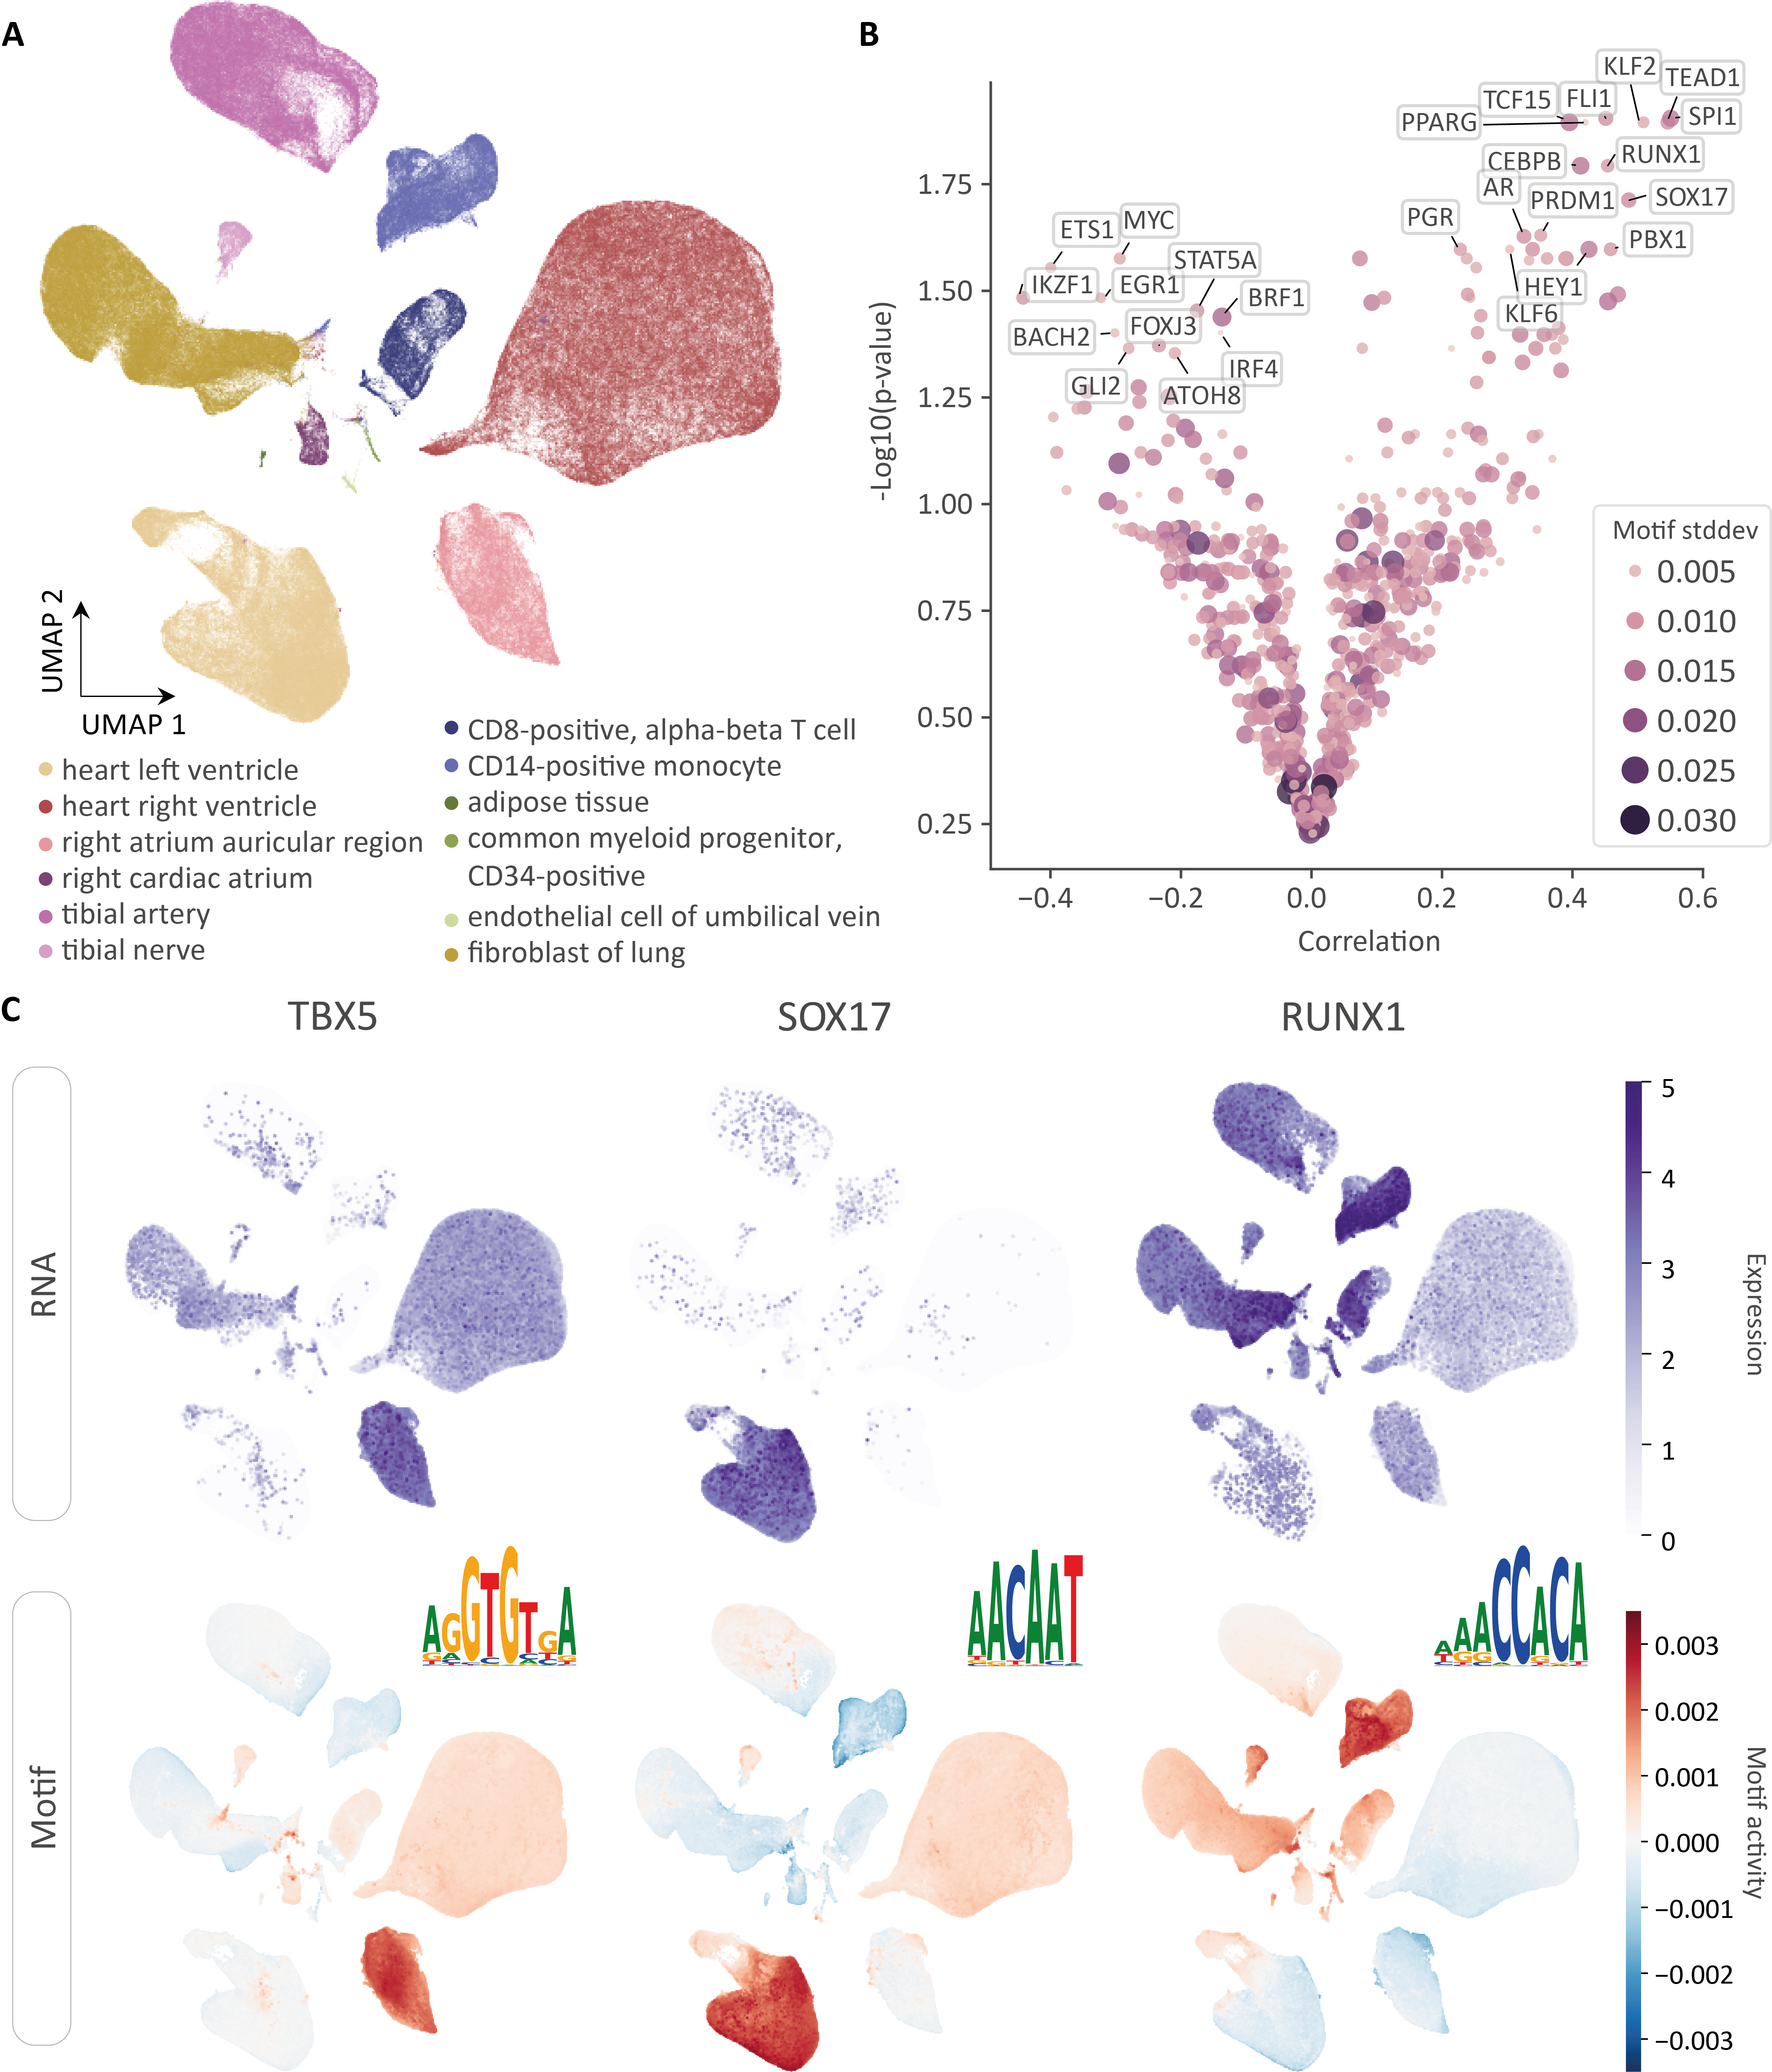
\includegraphics[width=0.75\linewidth]{ch.scepia/imgs/SCEPIA_allCells_Fig1_v9.png}
    \caption{\textbf{SCEPIA run on the Human Heart Cell Atlas} (a) UMAP representation, based on UMAP coordinates provided by the original study\cite{Kanemaru2023}, with cluster annotation labels as predicted by SCEPIA. (b) Volcano plot of SCEPIA hits, labels of the top 15 of both correlating as anti-correlating hits are indicated, based on p-adj < 0.05 values. Dot size and color labels are based on the motif score standard deviations.  (c) Expression levels (top) of 3 well-known markers, TBX5 (cardiomyocytes), SOX17 (endothelial cells), RUNX1 (blood cells), and their predicted motif [[scores/activity]] by SCEPIA (bottom), printed on the UMAP as shown in (a). Sequence logos of the binding motifs are indicated, with the GimmeMotifs database identifiers (left to right): GM.5.0.T-box.0005, GM.5.0.Sox.0021, GM.5.0.Runt.0003. }
    \label{fig:scepia_hhca1}
\end{figure}

\textbf{Benchmark SCEPIA on Single-Cell Data}

Next, we set out to more broadly assess SCEPIA's results, as well as its reproducibility. To this end, we split up the hHCA scRNA-seq data into seven random subsets of 100K cells each. Simultaneously, we ran GimmeMotifs Maelstrom motif analysis on the pseudobulk of the scATAC-seq clusters (from now on referred to as maelstrom analysis), to explore cell-type specific motif activities in the measured accessible regions. SCEPIA is designed to infer enhancer activity and this motif analysis on pseudobulk scATAC-seq therefore functions as the closest approximation to a \textit{ground truth} for this experiment. We correlated the motif activities computed from the maelstrom analysis with the expression levels of each of their TF binders per cell type, and for each subset. This comparison is done without any prioritization between motifs and TFs, other than taken into account the information on predicted motif-binding factor links, and we therefore refer to this as the naive comparison. The naive comparison resulted in coefficients ranging from r = -0.03 to 0.27 (Fig. \ref{fig:sc_benchmark} blue) \textcolor{red}{and represents the degree of similarity between motif activities and the expression levels of its binding TFs, taken from the best matching multimodal data source.}

To benchmark SCEPIA against these results, the analysis on each of the seven subsets were compared to the maelstrom analysis. The significant hits (p-adj < 0.05) were selected and their inferred motif activities averaged per cell type. These averages were correlated to the computed activities for the same motifs from the maelstrom analysis. Interestingly, the mean coefficients per cell type in these correlations, were consistently higher (up to r = 0.6 for the myeloid cluster) than found with the naive comparison, except for the mesothelial cell cluster (Fig. \ref{fig:sc_benchmark} orange). However, these scores differed substantially across the different cell types.

Since some of the cell types appeared to score worse (cardiomyocyte clusters, fibroblastst and endothelial cells, averaged r < 0.4), than others (immune cell cluster, averaged r > 0.4), we added a step to achieve better representation of each cell type in the data. This was done by adding a step of geometric sketching (geosketch) in the pre-processing of the data (REF XX \& \href{https://www.cell.com/cell-systems/fulltext/S2405-4712(19)30152-8}{https://www.cell.com/cell-systems/fulltext/S2405-4712(19)30152-8}) (see Methods), and before SCEPIA was run on each of the seven subsets. This improved the correlation coefficients with the maelstrom results of most cell types - even the immune cell clusters, but especially of the cardiomyocyte, fibroblast and endothelial clusters (Fig. \ref{fig:sc_benchmark} green). The neural and adipocyte, mural and mesothelial cell-clusters achieved more variability in their coefficients, obtained equal or worse coefficients after addition of the geosketching, respectively. \textcolor{red}{Although the geometric sketch was not able to alleviate SCEPIA's issues with some cell types,} adding this step to pre-processing did improve the tool's performance for the majority of the cell clusters. 
\begin{figure}
    \centering
    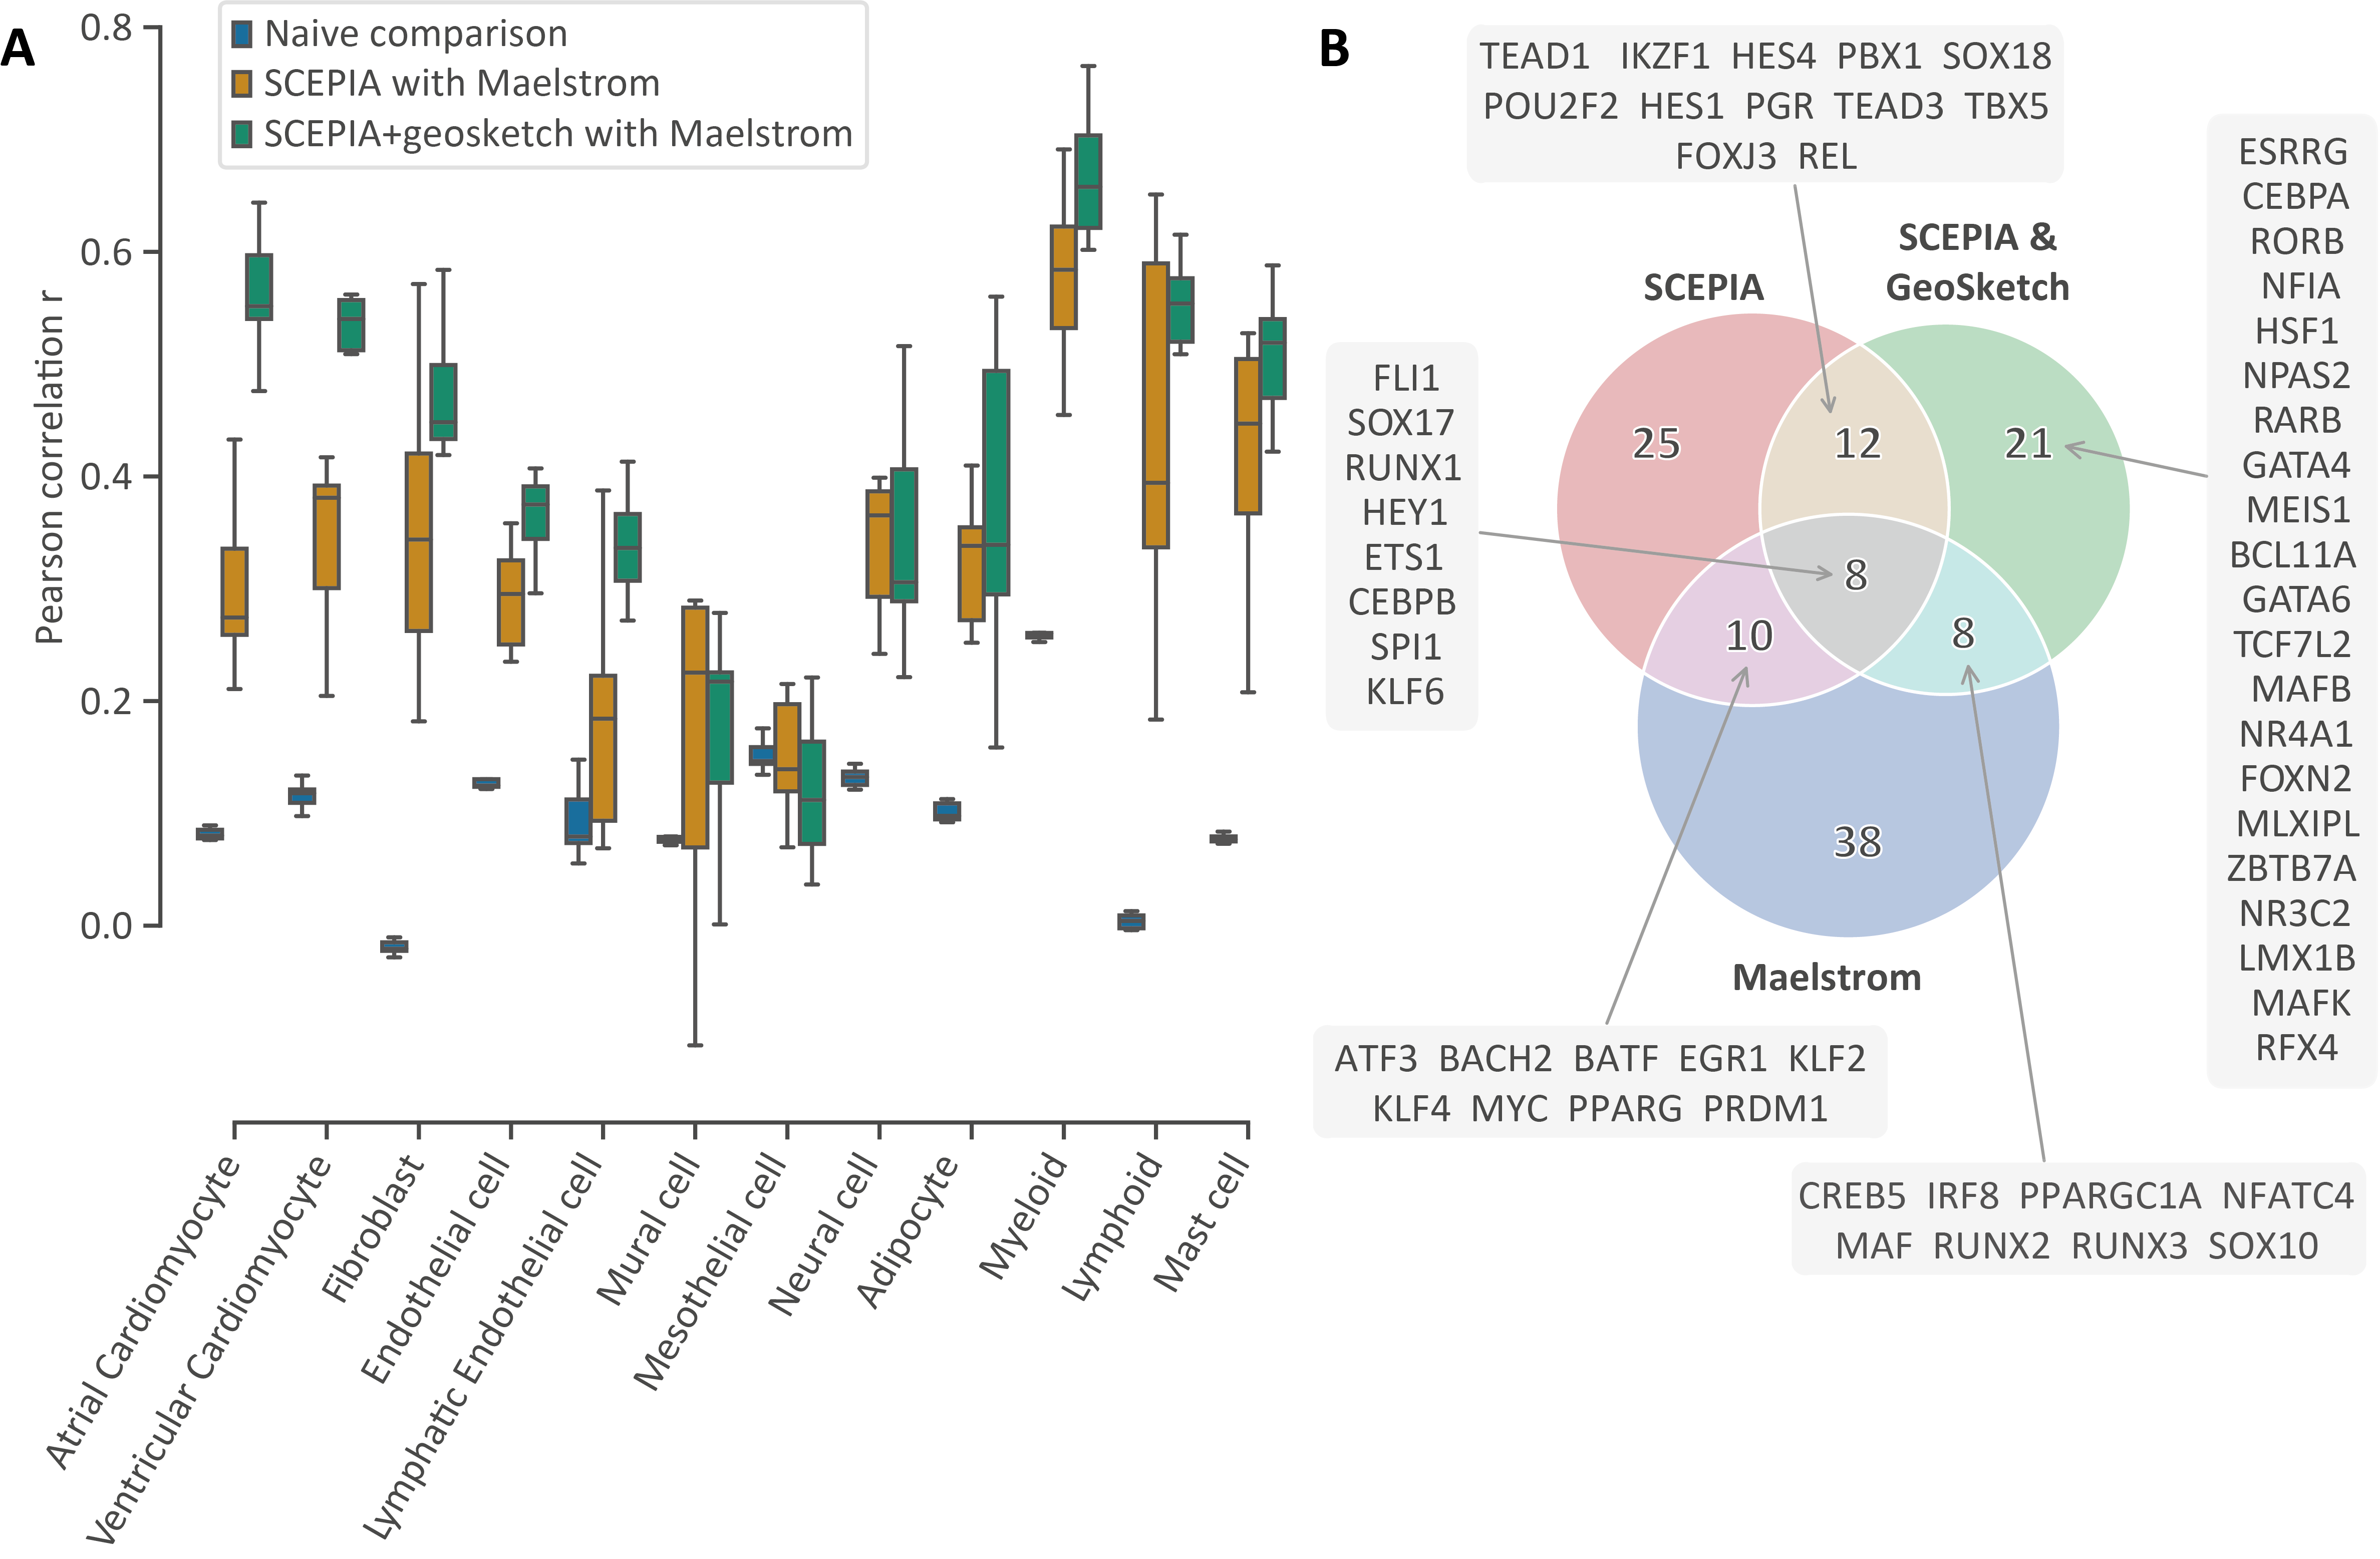
\includegraphics[width=0.75\linewidth]{ch.scepia/imgs/Fig_OverlappingHitsBetweenSCEPIAGEOANDMAELSTROM_v7.png}
    \caption{SCEPIA sc benchmark vs Naive vs Geosketch}
    \label{fig:sc_benchmark}
\end{figure}

\textcolor{red}{\textbf{Comparison of Biological Findings Across the Methods // Comparing SCEPIA with Maelstrom Motif Activities} }
Since the geosketch improved SCEPIA's performances across multiple cell types, we also reduced the full dataset to a sketch of 20K cells and reran SCEPIA (Fig. \ref{fig:geoscepia_results}). This resulted in overlapping hits with the former run of SCEPIA on the full dataset (20 hits of the 49 total hits), partial overlap with TFs linked to motif hits identified with maelstrom (16 hits; Figure 4B). Multiple overlapping hits between both SCEPIA runs on the full dataset and the maelstrom analysis, are known for their roles in cardiac cells, again FLI1 and SOX17 were present in all analyses, as well as HEY1 (cardiac progenitor marker) and ETS1 (lymphoid marker). Another example found in the first SCEPIA run and identified as a repressor, was BACH2. Maelstrom analysis also pointed to differential accessibility for a BACH2-binding motif and indicated enrichment in the fibroblast, endothelial and mesothelial cluster. SCEPIA also inferred increased motif accessibility for BACH2 in these same clusters, with additional enrichment in the myeloid and mural cells (Figure S4XX). 

However, there were also differences between the two SCEPIA runs. For instance, different GATA4 and GATA6 both known for their roles in cardiac (mesoderm) development and indicated with increased motif accessibilities in the cardiomyocyte clusters, were only identified after performing the geosketch (Figure \ref{fig:scepia_features1}A-B; \href{https://pubmed.ncbi.nlm.nih.gov/8660897/}{https://pubmed.ncbi.nlm.nih.gov/8660897/}, \href{https://www.ncbi.nlm.nih.gov/pmc/articles/PMC8916722/}{https://www.ncbi.nlm.nih.gov/pmc/articles/PMC8916722/}). In the run without geosketch, SCEPIA identified only GATA1 which showed a combination of specific expression and motif enrichment in mast cells,\textcolor{red}{ a link that can be made based on literature (\href{https://pubmed.ncbi.nlm.nih.gov/12566412/}{https://pubmed.ncbi.nlm.nih.gov/12566412/}; \href{https://ehoonline.biomedcentral.com/articles/10.1186/s40164-015-0024-z}{https://ehoonline.biomedcentral.com/articles/10.1186/s40164-015-0024-z}).} Besides this, RUNX1 was identified in both runs and in maelstrom. Specifically in the geosketch SCEPIA analysis RUNX2 and RUNX3 were added to the list, and the predicted motif for all of these factors (Runt.0003) was in the run with geosketch more restricted to immune cells, whereas in the other SCEPIA run the motif accessibility was also spread across for instance, the mural, neural and fibroblast cells (Figure \ref{fig:scepia_features1}C-D). 

Also some specific geosketch SCEPIA hits overlapped with the variable motifs as identified in the maelstrom analysis. PPARGC1A is an example of this and the exact same motif SCEPIA picked up, was identified to be variable in the maelstrom analysis (C2H2\_ZF.0037). Furthermore, the pattern of activity for this motif overlapped between the two methods, with stronger enriched in the adipocyte, fibroblast and myeloid cluster (Figure \ref{fig:scepia_features1}E, G). Motif activity of PPARGC1A is highest in adipocytes, endothelial and fibroblast cluster, as both identified with SCEPIA and Maelstrom, whereas the expression is found highest in the cardiomyocyte clusters. This is why SCEPIA identified PPARGC1A as a repressor. Another example concerns the SOX gene family. SOX17 and SOX18 were already identified in the first SCEPIA run, coupled to motifs with similar accessibilities over the clusters, additionally SOX13 was identified in that run (Figure \ref{fig:scepia_features1}F). SOX10 however, was only identified in the run pre-processed with geosketch, and was specifically expressed in the neural cluster (Figure S4XX). In the maelstrom analysis, two in the top three highest enriched motifs of the neural cluster, concerned motifs for SOX10 (Sox.0018 and Sox.007), with highest accessibility in the neural cluster, \textcolor{red}{followed by the fibroblast cluster for the one motif and by the endodermal cells in the other}. In the SCEPIA analysis the predicted motif for SOX10 (Sox.0034) showed this same level of specificity of enrichment (Figure \ref{fig:scepia_features1}H).

Differences between the maelstrom analysis and SCEPIA runs, included IKZF1, which was picked up by SCEPIA and linked to a motif with abundant accessibility and only a specific depletion of signal in the immune clusters (Fig. \ref{fig:scepia_features2}B, D). Other examples include, TBX5 and MEIS1, both well-known cardiac mesoderm markers, alongside ESRRG. Some of the binding motifs for these factors, according to the predictions, showed a level of activity across multiple clusters in the dataset, and only in combination with their expression made these factors more specific as potential transcriptional regulators (example of ESRRG, Fig. \ref{fig:scepia_features2}A, C). Conversely, there were also hits in Maelstrom, that were not identified in any of the SCEPIA runs. The MEF2 transcription factor family showed a specific motif enrichment in the accessible chromatin of the cardiomyocyte and mural cell cluster, however, the expression levels for MEF2A-D were very consistent over the different cell types in the dataset, which could explain this result (Fig. \ref{fig:scepia_features2}E).

\section{Discussion}

In this study, we present SCEPIA, a computational method for the inference of transcription factor motif activities based on transcriptomic data and a reference H3K27ac collection. We show that one can reliably match cell types based on transcriptomic abundance and H3K27ac-based regulatory potential\cite{Wang2016}, both in the case of bulk and single-cell transcriptomics. The chromatin context of the matched data can be used for motif activity inference, which in turn can be integrated with transcriptomic information. As such it is a big improvement over the case when only transcriptomic data is available. We test the inferred \textbf{regulatory} transcription factors on the human heart cell atlas, and show that XYZ. Altogether we ...

Section HHCA?

Although SCEPIA 

Another point to consider is the difficulty in accurately benchmarking these results and the establishment of an accurate ground truth. First, accurately inferring \textbf{regulatory} transcription factors by regression is just a method\cite{FANTOM2009,Balwierz2014,Madsen_2017}. These motif activity scores. Moreover, this approach is sensitive to the selected peak set, something we tried to explore in fig benchmark (\textbf{TODO}). Second, for the single-cell comparison, we compare the motif activities of scepia, which are based on bayesian ridge regression, to the motif activities of gimmemotifs\cite{Bruse_2018}. The motif activities of gimmemotifs are based on an ensemble of methods, and as such the ground truth is polluted by the difference in methods. Finally, in the single-cell comparison we compare single-cell ATAC-seq to bulk H3K27ac. These assays measure different things, for example, nuclear receptor motifs may not be necessarily associated with differential accessibility, if these factors bind in pre-existing accessible regions to regulate enhancer activity. 

At first glance, there is a seemingly large overlap between the approach of SCEPIA with SCENIC\cite{Aibar_2017}. However, there are important differences in the implementations. SCENIC starts by forming gene regulatory networks based on co-expression alone. These networks are then refined based on whether the DNA-binding motifs of TFs are present in the cis-regulatory regions of the downstream genes. SCEPIA conversely matches the transcriptome against reference H3K27ac, and infers motif activities on those, and relates the motif activities to gene counts. This seemingly small difference has major implications for the inferred motifs. The motif activities of SCEPIA are thus always based on possible combinations, as measured. This has the advantage that SCEPIA does not imagine certain relations. However, this also has the clear disadvantage that SCEPIA can not infer gene relationships that are not present in its database, something that SCENIC is able to do. A direct comparison between these tools would be nice. But this is diffucult because of technical stuff like different motif and transcription factor database. Moreover, these comparisons are highly influenced by the chosen ground truth. If we would use our regression-based ground truth probably SCEPIA better because it is regression-based. As such these methods are probably complementary.

Integration of multiple sequencing assays would be nice

Other databases supported (e.g. mouse and ATAC)

Regulatory potential can be matched.
- also in cases where the tissue type is not a 100 percent match (lung fibroblasts for heart fibroblasts for instance).

Summary of the good.
- Beter dan hoe het alleen op expressie data de TFs te identificeren zouden zijn.

Separation of train/test/validate bcz bulk vs sc?

\begin{itemize}
    \item No use of scATAC-seq in SCEPIA: new "standard". Can be rephrased as positive. Scepia H3K27ac is complementary to scATAC-seq
    \item Only 1 tissue type tested in this story. (Refer to Onecut2?)
    \item scData general struggle: Difficulty in picking the right peaks and genes that explain all \textit{important} heterogeneity/variability in the dataset.
    \begin{itemize}
        \item GeoSketch improved on this, ideas for further improvement?
        \item Some cell types are missing in the reference, therefore these likely stayed low in their correlations.
        \begin{itemize}
            \item How well are mixtures of cell types able to recapitulate an unknown/absent cell type? > it is not, doesn't work. but: 
            \begin{itemize}
                \item SCEPIA took from the top 50 cell type matches over the whole dataset, all of the weights per single cell along in computing the motif activities, meaning it did not only considers the highest match, which was helpful for some of these mismatches, or for cell types absent in the reference. // Talk about mixed signatures.
            \end{itemize}


        \end{itemize}
        \item \end{itemize}

        \item Explain differences between Maelstrom and SCEPIA: 
        \begin{itemize}
            \item \textcolor{red}{Is the regression used to perform motif enrichment, not the same?}
        \end{itemize}
\end{itemize}


\subsection{Limitations}
\begin{itemize}
    \item Benchmark is bad. Benchmarking against a bad ground truth is stupid.
    \begin{itemize}
        \item maelstrom vs lasso regression
        \item Naive TF-motif comparison as ground truth; in SCEPIA comparison we only take 20-100 significant hits to perform the correlations with.
        \item How to establish a good "maximum correlation"/"ground thruth", to compare SCEPIAs outcome with.
    \end{itemize}
    \item Can not detect alternative splcing / rna degradation / post translational modifications etc.
    \item No integration of target gene information

\end{itemize}

\section{Methods}

\subsection{Overview of public data}

\subsubsection{Sequencing data}

Table RNA-seq
96  RNA-seq cell types (accession + cell type)
 
Table H3K27ac
121 human H3K27ac cell types (Accession + cell type)

\subsubsection{Cis-regulatory regions}

We used a collection of cis-regulatory regions, based on all human transcription factor ChIP-seq peaks from ReMap 2018\cite{Chneby2017} (\url{http://remap.univ-amu.fr/storage/remap2018/hg38/MACS/remap2018_all_macs2_hg38_v1_2.bed.gz}), as described previously\cite{Xu_2020}. This collection of cis-regulatory regions is available at Zenodo with doi 10.5281/zenodo.4066423.

\subsubsection{Human heart cell atlas}

[Description]

\subsection{RNA-seq processing}

Preprocessing of RNA-seq was done automatically by seq2science v1.0.3 \cite{seq2science} using the RNA-seq workflow. Public samples were downloaded from the Sequence Read Archive \cite{Leinonen2010} with the help of the NCBI e-utilities and pysradb\cite{Choudhary2019}. Genome assembly GRCh38.p13 was downloaded with genomepy 0.16.1 \cite{Frlich2023}. Paired-end reads were trimmed with fastp v0.23.2 \cite{Chen2018} with default options. Reads were aligned with STAR v2.7.10b \cite{Dobin2012} with default options. Afterwards, duplicate reads were marked with Picard MarkDuplicates v3.0.0 \cite{picard}. BAM files were converted to CRAM format with samtools v1.16 \cite{Danecek2021}. Read counting and summarizing to gene level was performed on filtered BAM files using HTSeq-count v2.0.2 \cite{Anders2014}. TPM-normalized gene counts were generated using genomepy based on longest transcript lengths.

\subsubsection{H3K27ac ChIP-seq processing}

Then align all human h3k27ac from ENCODE to remap peaks. qnorm \cite{qnorm}
[expand]

\subsection{Regulatory potential}\label{section:regpotential}

The cell type-specific regulatory potential P of gene $g$ is calculated similar to\cite{Wang2016}:
\begin{equation*}
    P_g = \sum_k w_{k}s_{k,g}
\end{equation*}
where $w_k$ is the weight at position $k$, and $s_{k,g}$ is the h3k27ac signal at position $k$ for gene $g$.

\noindent
The weight $w_k$ is calculated identically to the method ANANSE\cite{Xu_2020}:
\begin{equation*}
    w_k = \begin{cases}
        1, & \text{if } k \in (0\,\text{kb},\ 5\,\text{kb}] \\
        \frac{2e^{-\mu|k-t_g|}}{1+e^{-\mu|k-t_g|}}, & \text{if } k \in (5\,\text{kb},\ 100\,\text{kb}]
    \end{cases}
\end{equation*}
where parameter $t_g$ is the genomic position of the TSS of gene $g$, and $\mu$ determines the decay rate as a function of distance from the TSS, set such that an enhancer 10 kb from the TSS contributes one-half of an enhancer within 5 kb from TSS. $t_g$ is the distance from the TSS.

\subsection{Regulatory motif analysis and motif and transcription factor activity}

In the regulatory potential benchmark (Fig. \ref{fig:bulk_comparison}B) and in SCEPIA we use the motif activity as a measure of motif and transcription factor importance. The motif activity\cite{FANTOM2009, Balwierz2014} is calculated using the Bayesian ridge regression implemented in gimmemotifs\cite{Bruse_2018}, with the motif log-odds scores as features and the H3K27ac signal as predictor variable. In short, for each cis-regulatory region in the input we compute the motif log-odds score for each motif in the gimmemotifs database (gimme.vertebrate.v5.0). This motif databases contains a non-redundant collection of vertebrate transcription factor motifs\cite{Bruse_2018}. We assume that the H3K27ac signal in each enhancer, expressed as log2(\# of reads + 1), is the sum of all motif log-odds scores multiplied by their respective motif weights. We then estimated these motif weights using lasso regression, where the regularization parameter ($\lambda$) was determined through 5-fold cross-validation. These motif weights, the feature coefficients from the fitted regression model, are used as a measure of motif importance, the motif activity. This measure can then be used as transcription factor activity based on the TFs that are predicted to bind to the motif.

\subsection{Benchmark of regulatory potential-based cell type and motif assignment.}

To assess the performance of the regulatory potential-based approach compared to the actual H3K27ac signal, we conducted a systematic analysis. Our approach involved data subsampling and calculating correlation coefficients to evaluate the relationship between the ground truth data and the regulatory potential-based approach. Specifically, this analysis utilized two data sources: the bulk H3K27ac reference database encompassing 121 tissues from ENCODE and 1,268,775 REMAP peaks, as well as the RNA-seq database featuring 96 tissues from ENCODE (\textbf{Table SX}).

To establish a ground truth for comparison, we calculated the motif activity using the top 25,000 enhancers with the highest coefficient of variation with GimmeMotifs version 0.18.0\cite{Bruse_2018}. We selected random subsets of five tissues from 5 tissues shared between the RNA-seq database and the H3K27ac reference database. The motifs were assigned to TFs, and we calculated the Pearson/Spearman correlation coefficients between the estimated motif activity and the ground truth motif activity for each tissue in each comparison.

In a naive approach to estimating motif scores, we consider the transcripts per million (TPM) of a transcription factor directly as the motif score. When multiple transcription factors are associated with a single motif, we use their mean.

In the regulatory potential-based approach, we exclude the five ground truth tissues from the reference database. We then convert the H3K27ac signal from the reference database into regulatory potential and subsequently perform regression analysis against the TPM values. This results in a 5 x XYZ table of regression weights. We select the top 50 tissues with the highest absolute regression weights and identify the top 10,000 differential enhancers between them. We then conduct a motif scan similar to the one performed for the ground truth, regressing the H3K27ac signal with the motif scores in these enhancers. Finally, the motif scores for our original five tissues are calculated by taking the dot product of the motif scores in the top 50 tissues and the tissue weights.

To assess the impact of using only the top 10,000 peaks for the regulatory-based approach while retaining the top 25,000 peaks for the ground truth, we also compute motif scores based on the top 10,000 differential enhancers (again selected based on coefficient of variation).

This entire process was repeated one hundred times to generate a distribution of correlation coefficients, providing an estimate of each approach's performance.

\subsection{Scepia}

The single-cell regulatory-based approach (scepia) is similar to the bulk approach. However, due to the enormous increase in data, some steps need to be altered from a computational resource point of view. In addition, the fact that a single-cell dataset usually consists of multiple related cell types, with a more fluent gradient in gene expression and thus motif scores, makes it so that this information can be used to infer the significance of differential transcription factors based on motif scores and gene expression data.

\noindent
Required input:

\begin{itemize}
	\item Reference database matrix of peak intensities (D) with dimensions (peaks x cell types). Scepia comes with multiple extensive reference databases, and the user does not need to provide them themselves. These reference databases can be extended, however.
    \begin{itemize}
        \item The default human reference is based on REMAP 2018\cite{Chneby2017}, and consists of 1,268,775 putative enhancers. It contains 121 ENCODE\cite{encode_dcc} cell types. The number of transcripts in these enhancers per cell line was log2(x+1) transformed, and quantile normalized\cite{qnorm} to enforce the same distribution.
        \item The default reference database is based on H3K27ac signal, but this can be any chromatin mark associated with transcription, for example, ATAC-seq.
    \end{itemize}
	\item Single-cell RNA-seq dataset S with dimensions (cells x genes). 
\end{itemize}

\noindent
Single-cell epigenome-based inference of activity can be divided into five main steps (see fig. \ref{fig:scepia_overview}):

\begin{enumerate}
    \item \textbf{Conversion of Reference Database Matrix into Regulatory Potential}
    
    Convert the reference database matrix of peak intensities $D$ into a database matrix of regulatory potential\cite{Wang2016} per gene $P$ with dimensions $(\text{genes} \times \text{cell types})$. The reference database includes all REMAP peaks, including promoters, and is prepared beforehand. See section \ref{section:regpotential} for a detailed explanation of the calculation of regulatory potential.

    \item \textbf{Cell Annotation from Single-Cell Dataset}
    
    Match cells in the single-cell dataset $S$ with regulatory potential $P$, resulting in an annotation matrix $A$ with dimensions $(\text{cells} \times \text{cell types})$. The transcript counts of each cell are regressed against the regulatory potential database. The annotation matrix represents the regression coefficients, and cells receive a tissue/cell type annotation based on the highest regression coefficient.
    
    \begin{itemize}
        \item The first step involves selecting a subset of relevant cell types to speed up the cell annotation. It assumes that the user has already performed Louvain or Leiden clustering, and averages the counts per cluster. The top 2,000 most variable genes (dispersion normalized) are chosen. For each cluster $c$, the regression coefficients are calculated by lasso regression:
        \begin{equation*}
            \underset{A_c}{\operatorname{argmin}}\ |S_c - P A_c| + \lambda |A_c|
        \end{equation*}

        Where the regularization parameter ($\lambda$) is estimated through 5-fold cross-validation.

        Absolute regression weights are summed per tissue/cell type, and the top 50 cell types/tissues are retained in the regulatory potential database.
        
        \item Mean center the single-cell counts and set each cell as the mean expression value of its neighbors. For each cell $i$, the regression coefficients are calculated using Bayesian ridge regression with the top 50 cluster weights:

        \begin{equation*}
            \underset{A_i}{\operatorname{argmin}}\ |S_i - P A_i|^2 + \lambda |A_i|^2
        \end{equation*}
        
        \item Cells are initially assigned the cell type/tissue with the highest weight, and clusters are annotated based on the most common cell type in that cluster. Cell types are further refined by taking the dot product of cell type weights with neighborhood weights. At least 50 cells need to be assigned a specific cell type; otherwise, they are labeled as "other".
    \end{itemize}

    \item \textbf{Motif Scan over Differential Enhancers}
    
    Select the to 10,000 enhancers with the highest variance between the annotated cell types. The resulting vector is denoted as $E$ and has dimensions (10,000 x 1). Infer the motif activities over these enhancers. 
    
    \begin{itemize}
        \item Only known motifs are considered. By default, the GimmeMotifs\cite{Bruse_2018} vertebrate v5.0 motif database is used.
        \item Scan and keep the maximal motif score in each enhancer. The result is a vector $O$ with dimensions (10,000 x nr of motifs).
        \item Motif weights ($M$) are calculated by Bayesian ridge regression:
        \begin{equation*}
            \underset{M}{\operatorname{argmin}}\ |E - O M|^2 + \lambda |M|^2
        \end{equation*}

        where the $M$ has dimensions (1 x nr of motifs).

        TODO check dimensions!

        \textbf{TODO}, the mean is subtracted here and I don't think it does anything meaningful... 
    \end{itemize}
    

    \item \textbf{Calculation of Motif Scores}:
    
    Calculate the motif scores for the cells based on the motif scores of the reference top tissues. The motif scores per cell are calculated as a dot product of the cell type annotation weight and motif scores per reference tissue / cell type.
    \begin{equation*}
        F = M \cdot A
    \end{equation*}
    TODO check dimensions!

    \item \textbf{Correlation Analysis of Motif and Transcript Scores}:
    
    Determine significant combinations by correlating motif scores ($F$) and transcript scores ($S$) between cells:
    \begin{itemize}
        \item Calculate the correlation coefficient between motif score and transcript counts.
        \item Randomly shuffle motif scores and calculate their correlation with transcript counts. Repeat this 100,000 times to obtain a distribution of correlation coefficients.
        \item Estimate two different p-values per TF-motif combination from this analysis: one based on the correlation coefficient relative to the total permuted set and another using only the permuted set of motif correlations. Combine these p-values using Fisher's method.
        \item Calculate motif activity by fitting a Gaussian mixture model with two components over the motif activity scores. These components represent "high" and "low" motif scores. Motif activity is computed as the probability that a motif score belongs to the "high" expressed group, and is thus constrained to the range of 0 to 1.
    \end{itemize}
\end{enumerate}

\subsection{Human Heart Cell atlas Single-cell comparison}
\textbf{Human Heart Cell Atlas single-cell comparison }
We have used the full global log-normalised counts-containing h5ad object of the human Heart Cell Atlas v2 (HCA) project as provided by the authors (\cite{Kanemaru2023}), and pre-processed the data with Scanpy (v1.9.2). Cell type assignment and UMAP-embeddings were used as provided by the authors. The dataset was subsetted to contain only highly variable genes (selected using the default settings within Scanpy; "min\_mean = 0.0125, max\_mean = 3, min\_disp = 0.5") and the normalized counts were scaled. Both the neighborhood connectivities of the single cells, as well as PCA were rerun, as necessary input for SCEPIA. SCEPIA's infer\_motifs was run on the preprocessed data with the following settings: using the top 2000 highly variable genes, the top 10,000 most variable enhancers and a maximum of 50 cell types from the reference, ridge regression was used for motif activity analysis and no subsetting on the number of cells was performed \textcolor{red}{(XX this I removed from the installation v0.5.1 -> not sure if this will be incoorporated in SCEPIA? PR is there XX).} The ENCODE H3K27Ac human reference dataset and gimme.vertebrate.v5.0.pfm motif file from the GimmeMotifs were used as input. The resulting data was visualized with seaborn v0.12.2, matplotlib v3.8.0 and gimme logo from GimmeMotifs (v0.18.0).

To establish how reproducible the SCEPIA runs are, and to benchmark the results by comparing with Maelstrom analysis, we split up the dataset into seven \textit{randomly selected} sets of 100K cells. Each of these subsets was preprocessed, by selecting and filtering on highly variable genes, scaling, selecting neighborhood connectivities and performing PCA analysis, as described above for the full dataset. Each of these subsets were used in seperate SCEPIA runs, also run with the same settings as above. 
- The same 7 subsets\textit{ as well as the whole hHCA dataset} underwent geometric sketching using geosketch (v1.2), prior to the SCEPIA analysis. First, the scaled data was used for PCA to enable the geometric sketching of 20K cells within the subset or full dataset. On the raw data the highly variable genes were selected and after scaling the data neighborhood connectivities selection, PCA and SCEPIA were performed//run in the same way as described before.
- // Similarly//In the same way, the full dataset was subsampled using geosketch to 20K cells on which SCEPIA was run again.

\textbf{Motif scanning on scATAC-seq fraction of Heart Cell Atlas}
The ATAC peak matrix object as provided by the authors, was normalized per cell for sequencing depth (multiplied by 10,000) and log1p transformed, the resulting dataset was averaged per cell type. Only peaks outside of promoter regions (2,000 bp up- and downstream of transcription start sites) were kept, to select for enhancer regions. The top 200,000 most variable enhancers were selected and the z-scores per peak and across the cell type means were calculated. The scaled matrix was used as input for gimme maelstrom from the GimmeMotifs package (v0.18.0), the same motif position frequency matrix file as used in SCEPIA (gimme.vertebrate.v5.0.pfm), and hg38 as the reference genome. Maelstrom results with a z-score > 3.5 in at least one of the cell types were selected for visualization in a heatmap. 
% -Question XX SELECT MOTIFS OF INTEREST FROM THIS ANALYSIS: what z-score threshold was used XX (Figure SXX). \textit{XX I did not select here for curated motifs only to create the venn diagram. Heatmap of MaelstromResults, plot_feature does seem to perform some filtering? XX}

\textbf{Benchmark SCEPIA with scATAC-seq motif analysis}
\textcolor{red}{XX ADD PREPROCESSING STEPS ATAC-seq DATA XX} For each of the seven scRNA-seq subsets of the HCA, the mean expression values per cell type were correlated with the mean motif scores per cell type of all its potential binding motifs, obtained from the Maelstrom analysis on the cell type-averaged scATAC-seq data. 
- This comparison is referred to as the Naive comparison. Only highly variable genes were selected for this analysis. 
- For the SCEPIA comparison, all significant hits from the analysis (p-adj < 0.05) were selected and the predicted motif activities were averaged per cell type. Predicted motif activities from SCEPIA were correlated with the activities of the same motifs as computed by Maelstrom, over the different cell types. // These inferred cell type motif activities were correlated with the activities predicted by Maelstrom analysis for each cell type. The same was done for the SCEPIA results of the geosketched subsets. Correlations in all of these comparisons were performed using the Pearson correlation method.

\section{Supplementals}
\beginsupplement
\begin{table}
    \begin{center}
        \begin{tabular}{||c c c c||} 
        \hline
        Weight curve & Correlation between & Correct specific & Correct broad \\[0.5ex] 
        \hline
        Ananse\cite{Xu_2020}& $0.53 \pm 0.14$ & $64\%$ & $77\%$ \\ 
        \hline
        Wang\cite{Wang2016} & $0.54 \pm 0.15 $ & $64\%$ & $75\%$ \\
        \hline
        Promoter (2kb) & $0.54 \pm 0.14$ & $66\%$ & $77\%$ \\
        \hline
        Enhancer & $0.43 \pm 0.14$ & $60\%$ & $72\%$ \\
        \hline
        Random & NaN & $2\%$ & $3\%$ \\
        \hline
        \end{tabular}
        \caption{\textbf{Something something.} Bla bla bla}
        \label{table:correlations}
    \end{center}
\end{table}

\begin{figure}
    \centering
    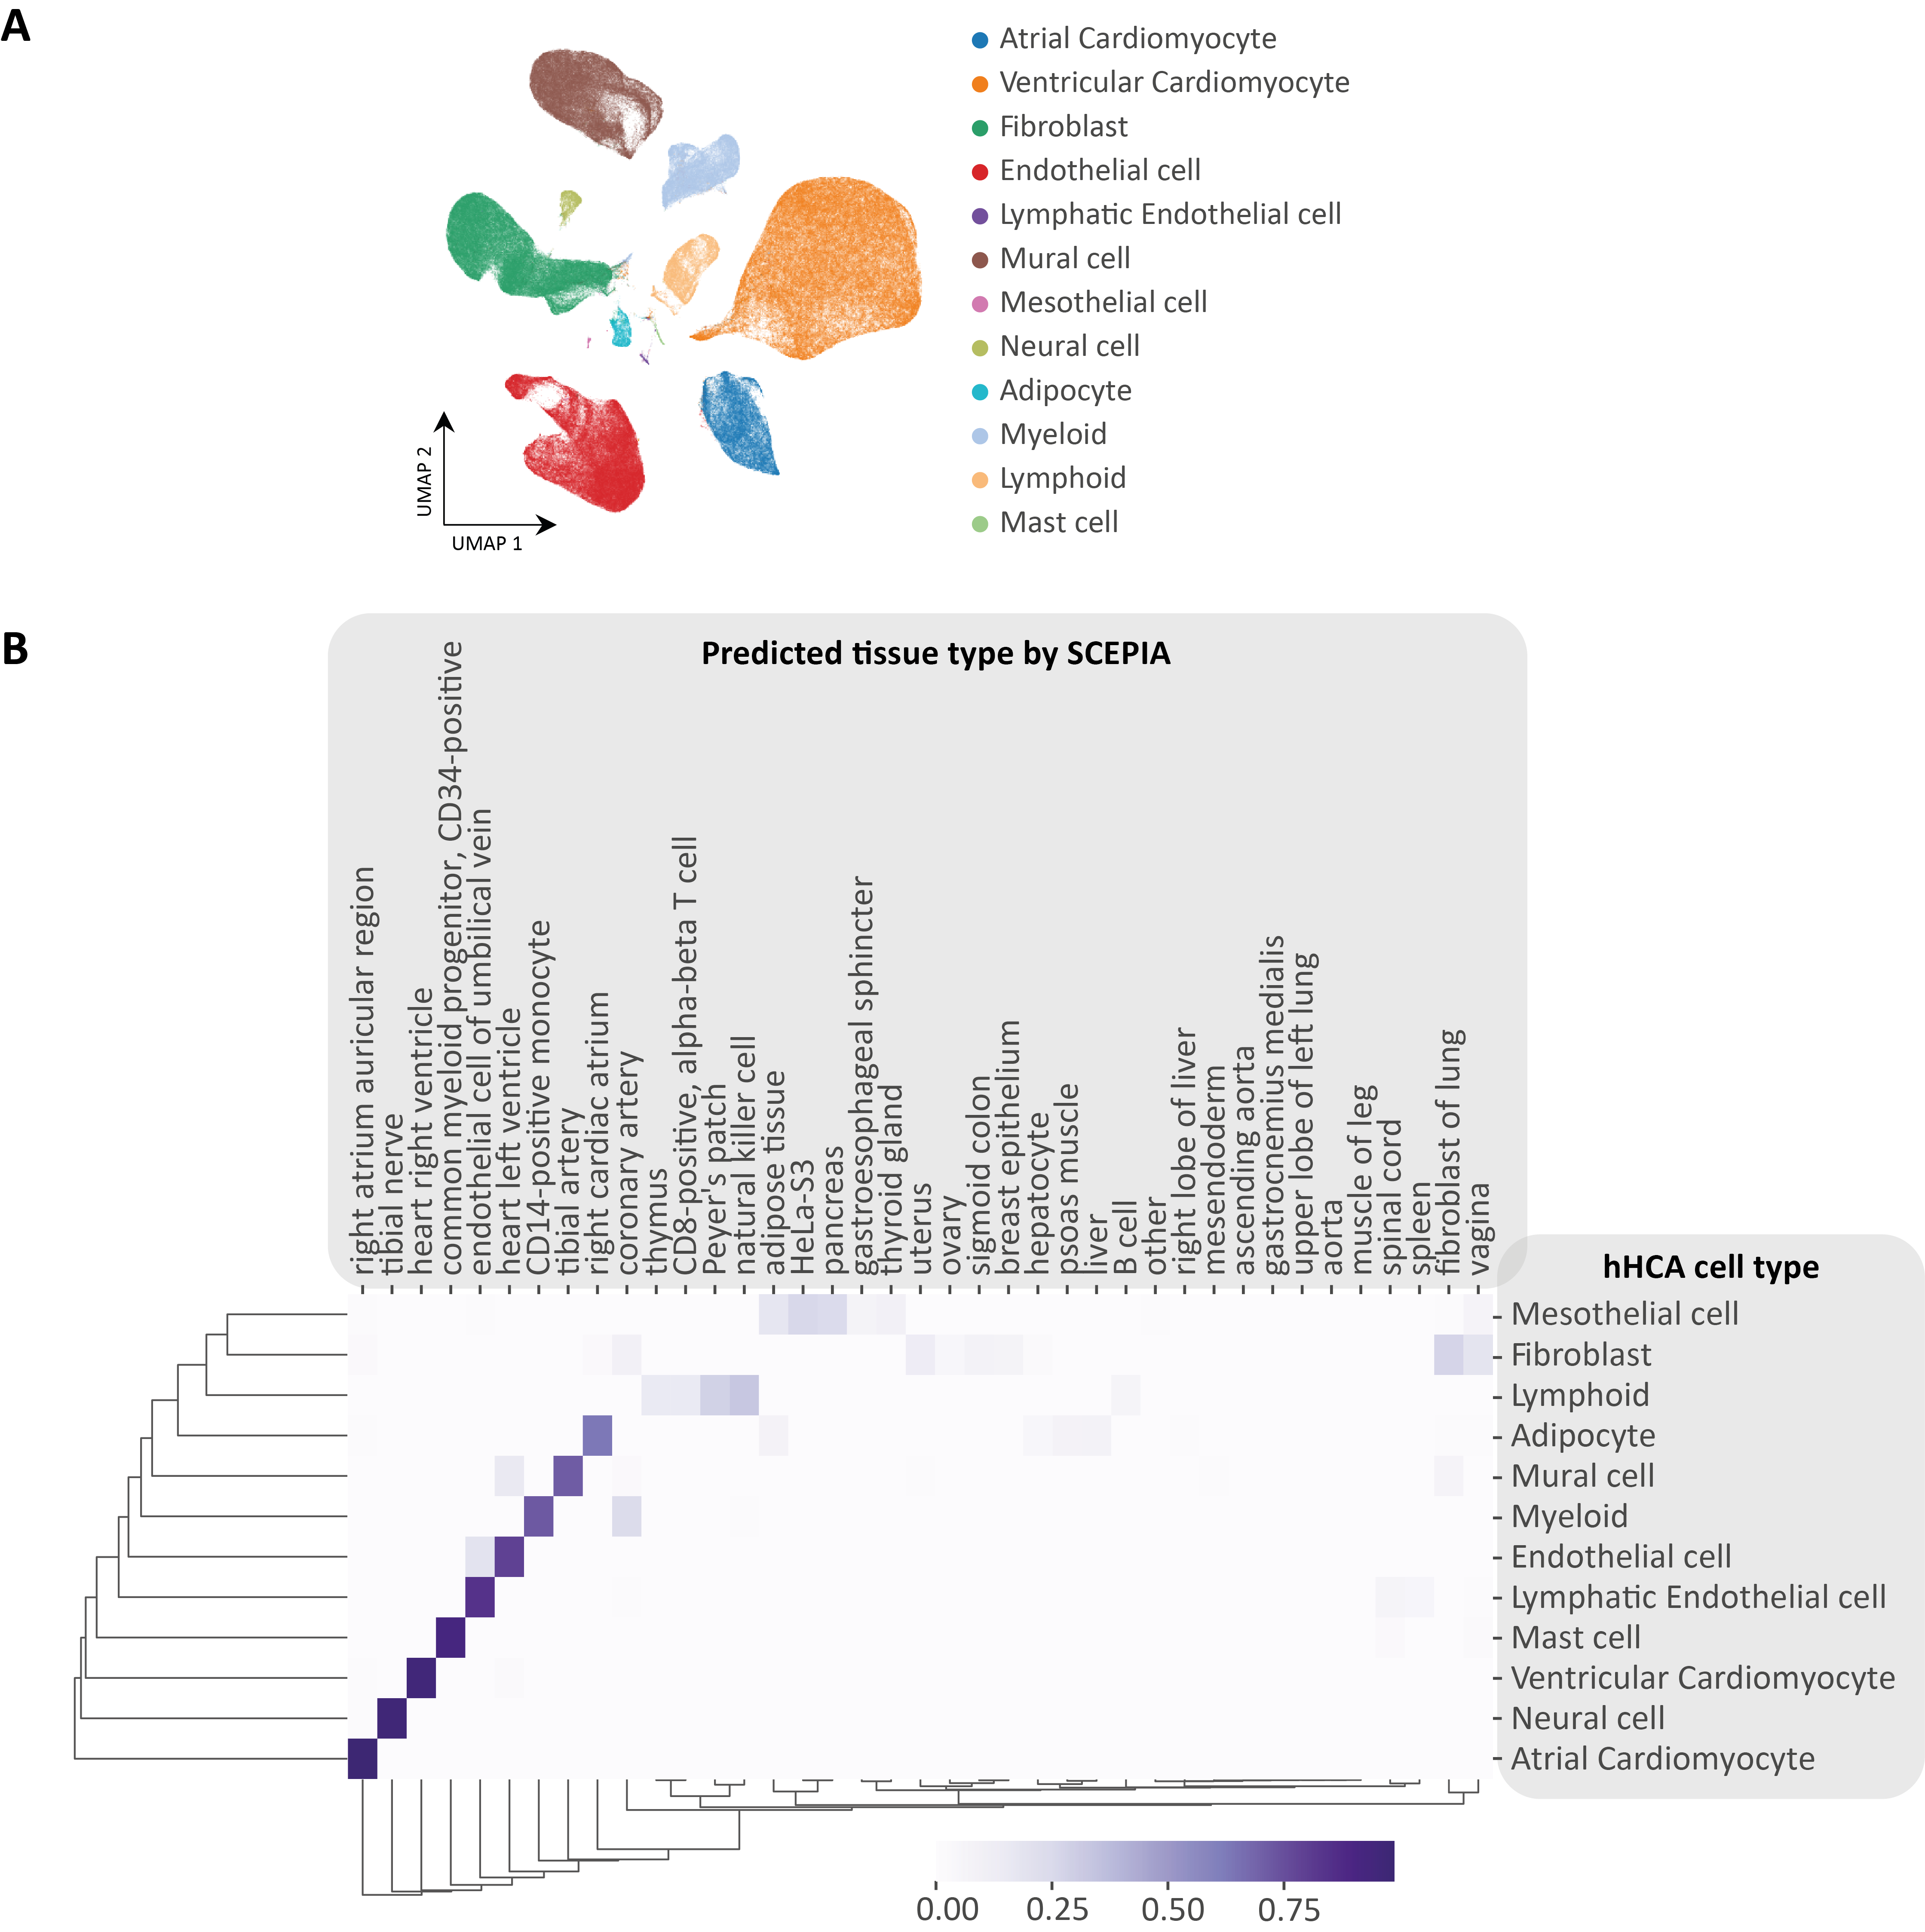
\includegraphics[width=\linewidth]{ch.scepia/imgs/SCEPIA_Annotation_allCells_SuppFig1_v4.png}
    \caption{Original annotation of cell types (a) SCEPIA annotation of clusters (b) Highest scoring motifs inferred with SCEPIA run on 700K cells (placeholder) }
    \label{fig:scepia_annotation1}
\end{figure}

\begin{figure}
    \centering
    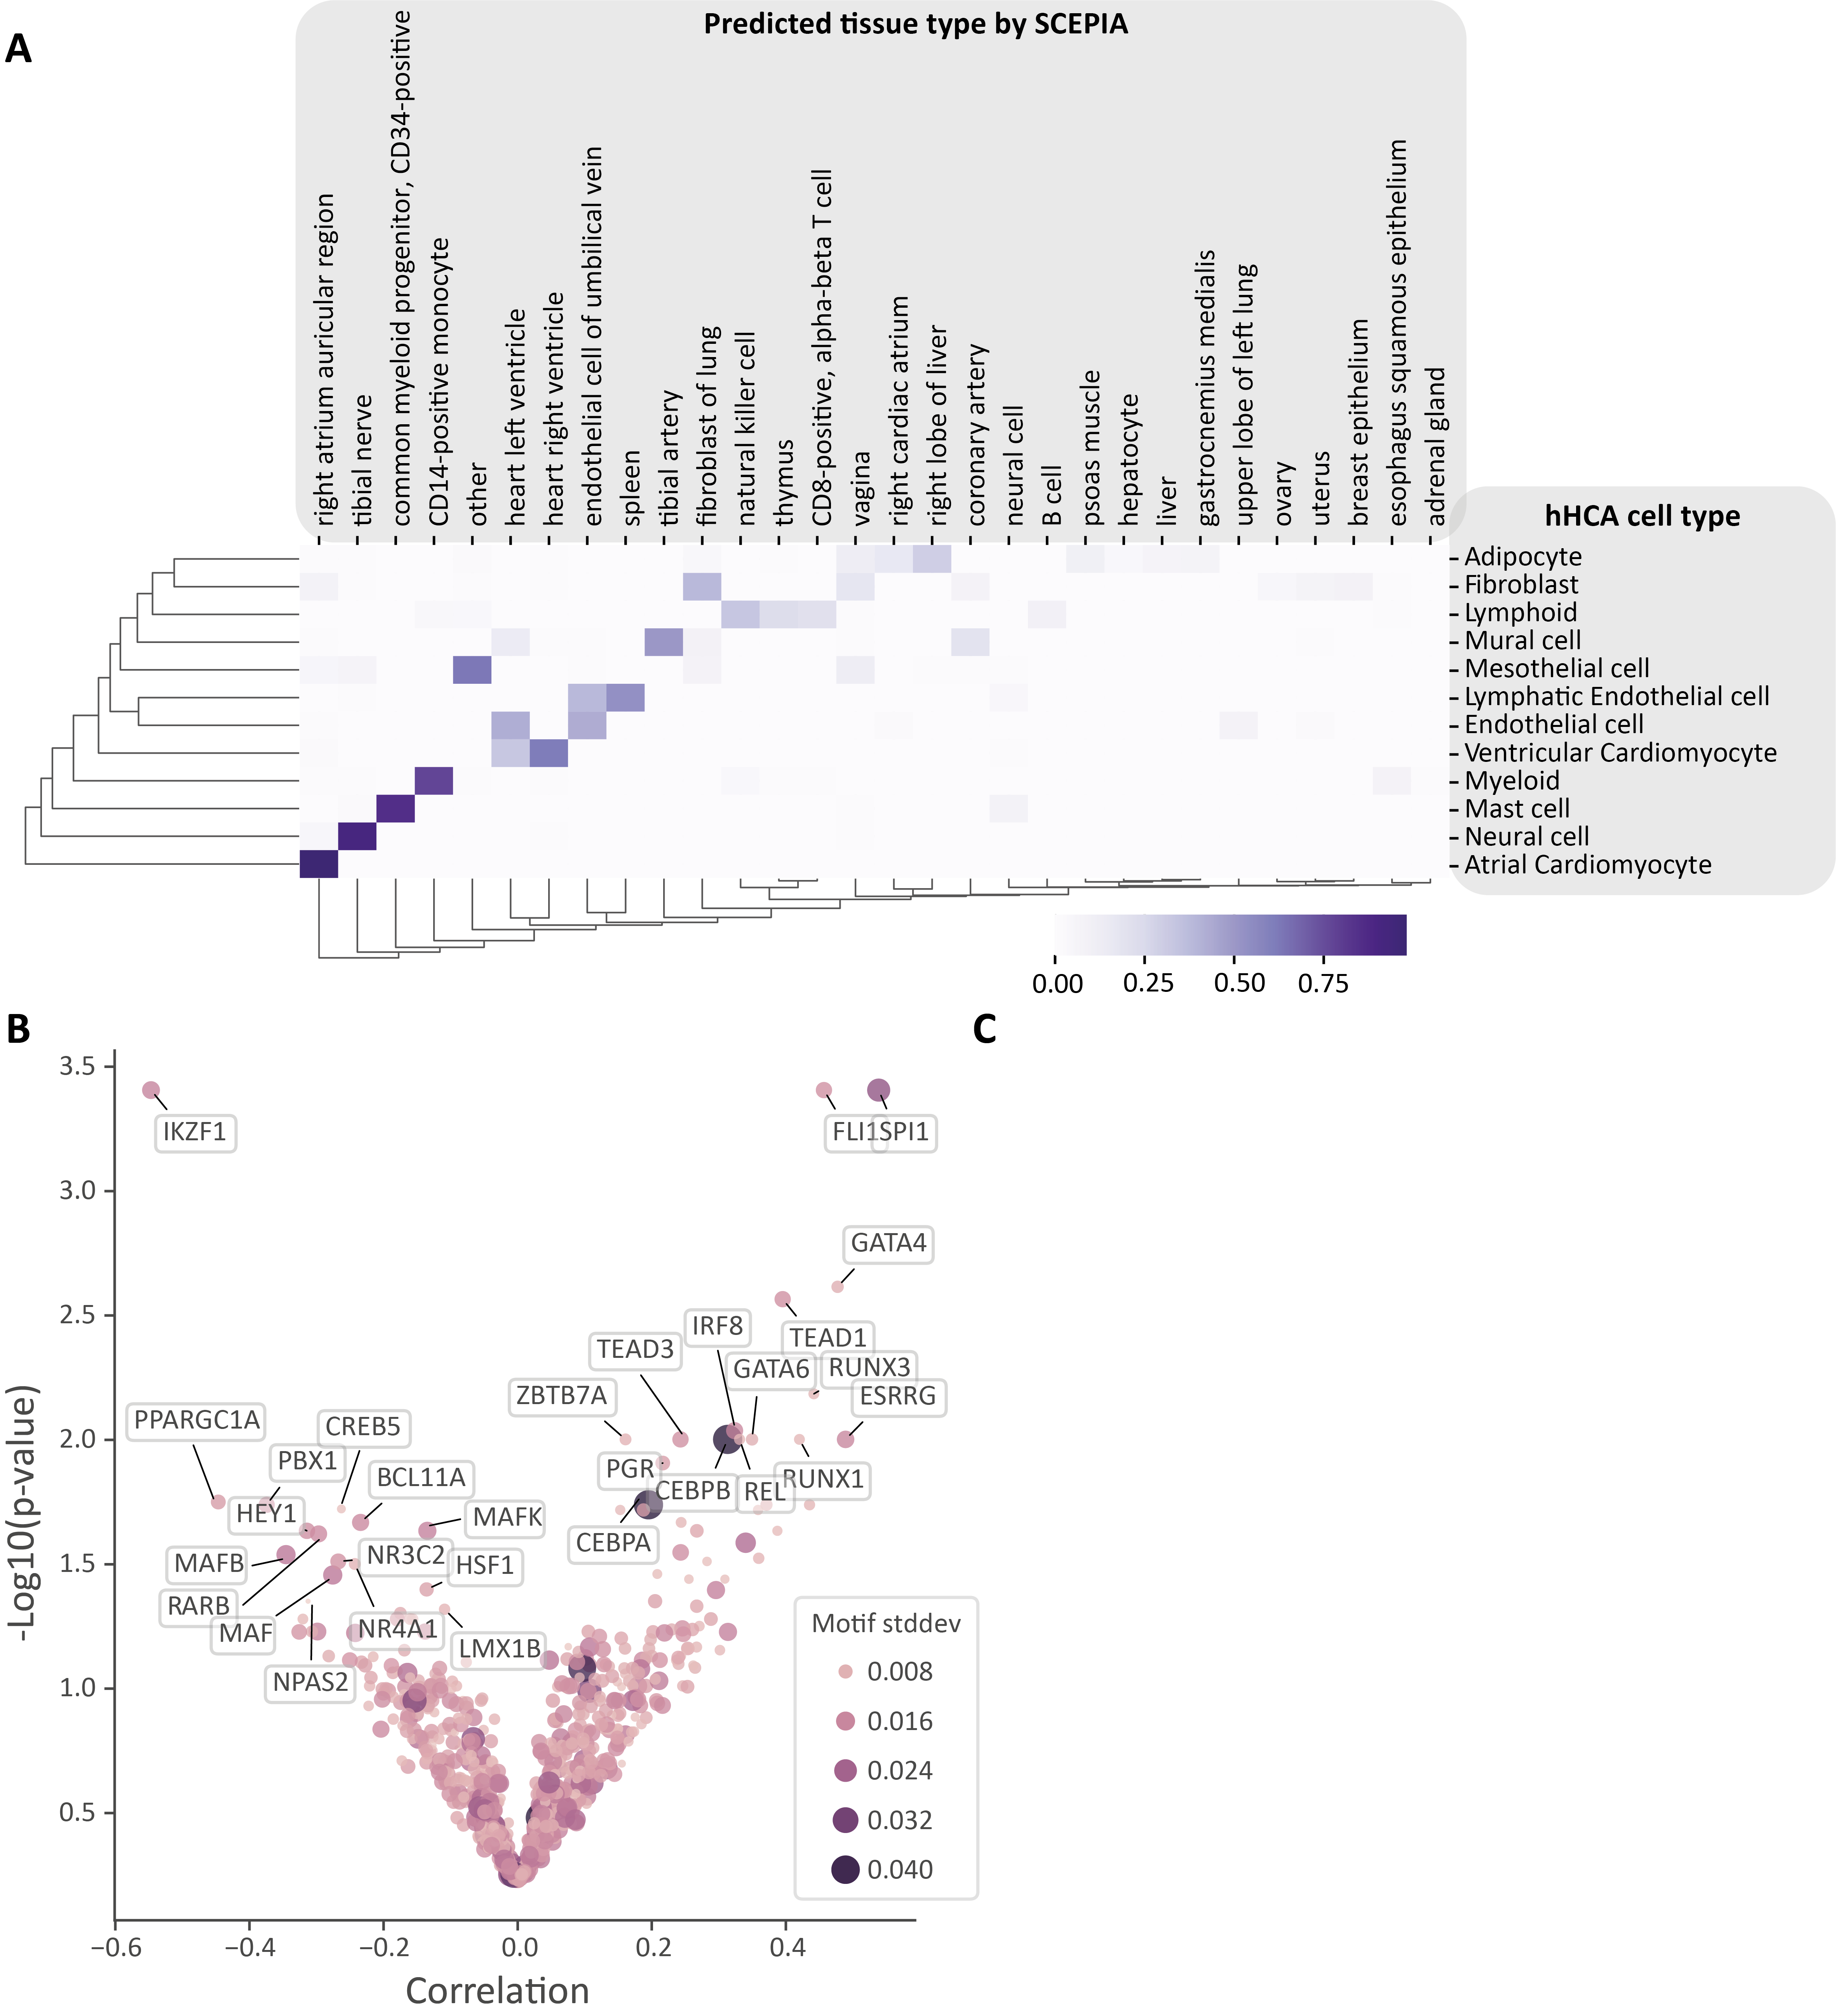
\includegraphics[width=\linewidth]{ch.scepia/imgs/SCEPIAGEOSKETCH_AllCells20000_Suppfig_v2.png}
    \caption{SCEPIA run on geosketch of hHCA (A) SCEPIA annotation of clusters (B) Highest scoring motifs inferred with SCEPIA run on 700K cells (C) (placeholder XX) UMAP of 20K geosketch hHCA. }
    \label{fig:geoscepia_results}
\end{figure}

\begin{figure}
    \centering
    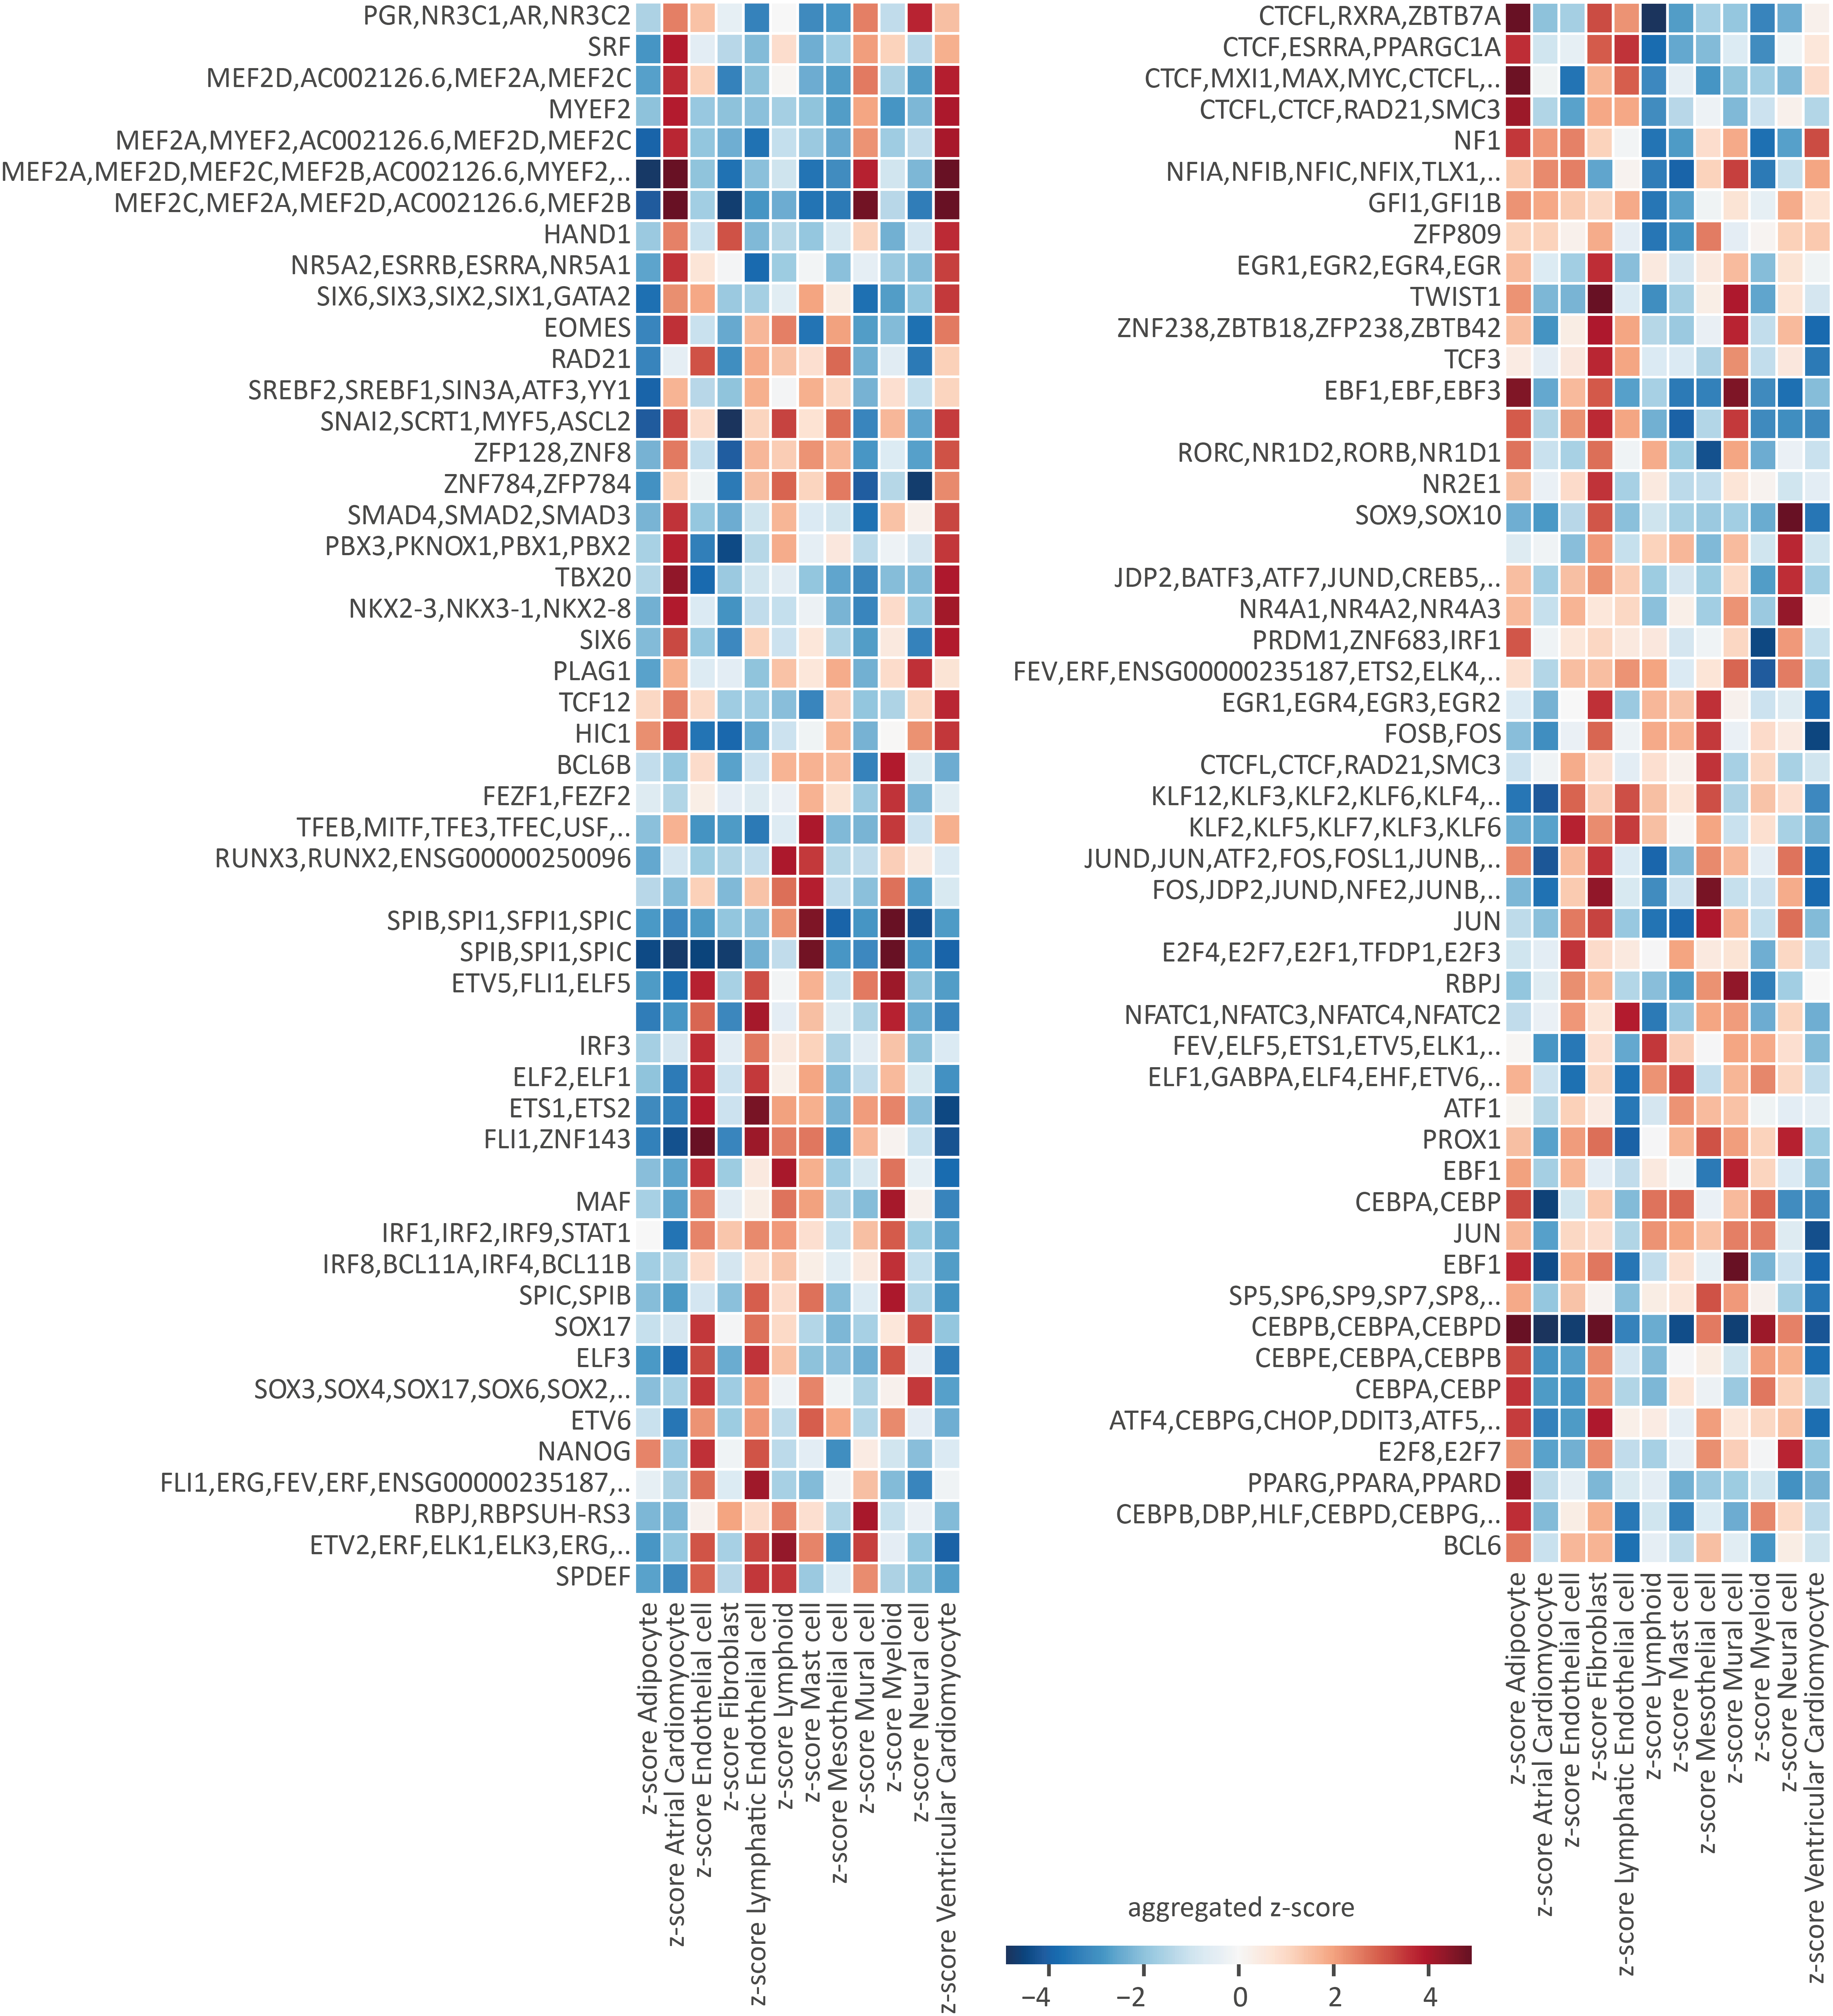
\includegraphics[width=\linewidth]{ch.scepia/imgs/Maelstrom_AllHitsAbove3.5.png}
    \caption{Maelstrom motif analysis output (z-score > 3.5) of the hHCA scATAC-seq cluster averages.}
    \label{fig:scepia_maelstromhm}
\end{figure}
\begin{figure}
    \centering
    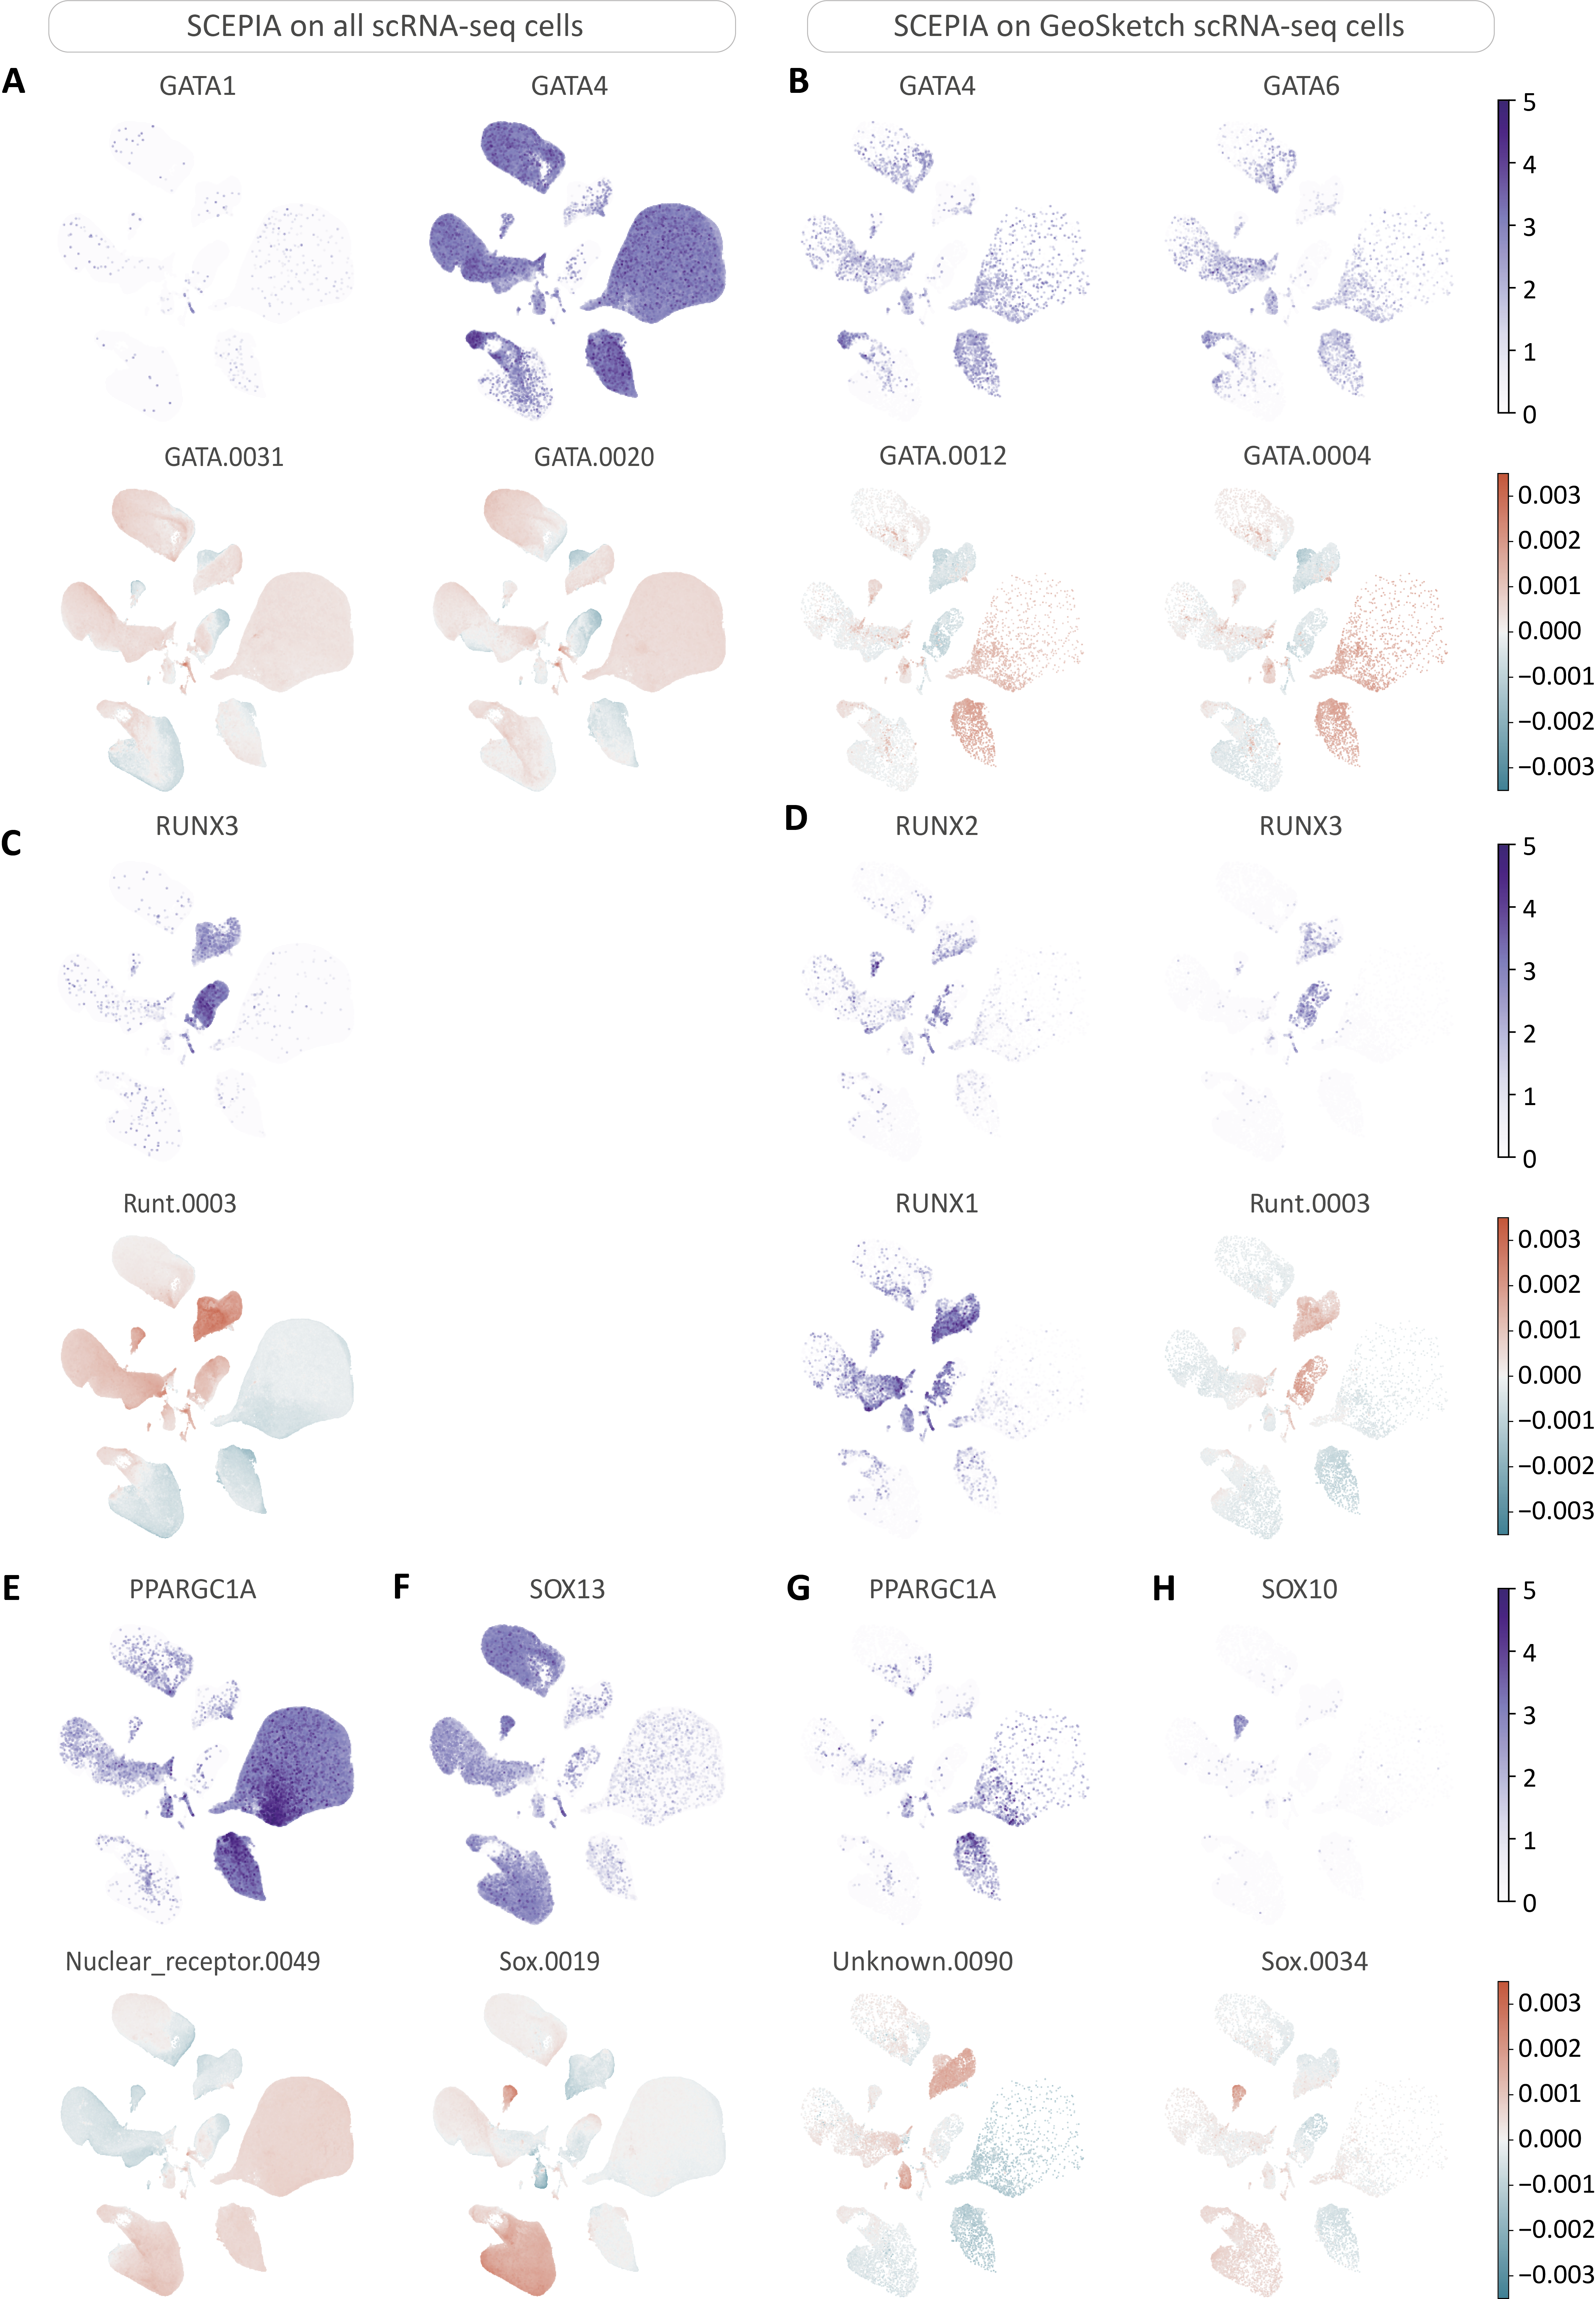
\includegraphics[width=\linewidth]{ch.scepia/imgs/SCEPIA_SCEPIAGEO_BiologicalExamples_SuppFig1_v2.png}
    \caption{Examples of SCEPIA and geosketch + SCEPiA run}
    \label{fig:scepia_features1}
\end{figure}

\begin{figure}
    \centering
    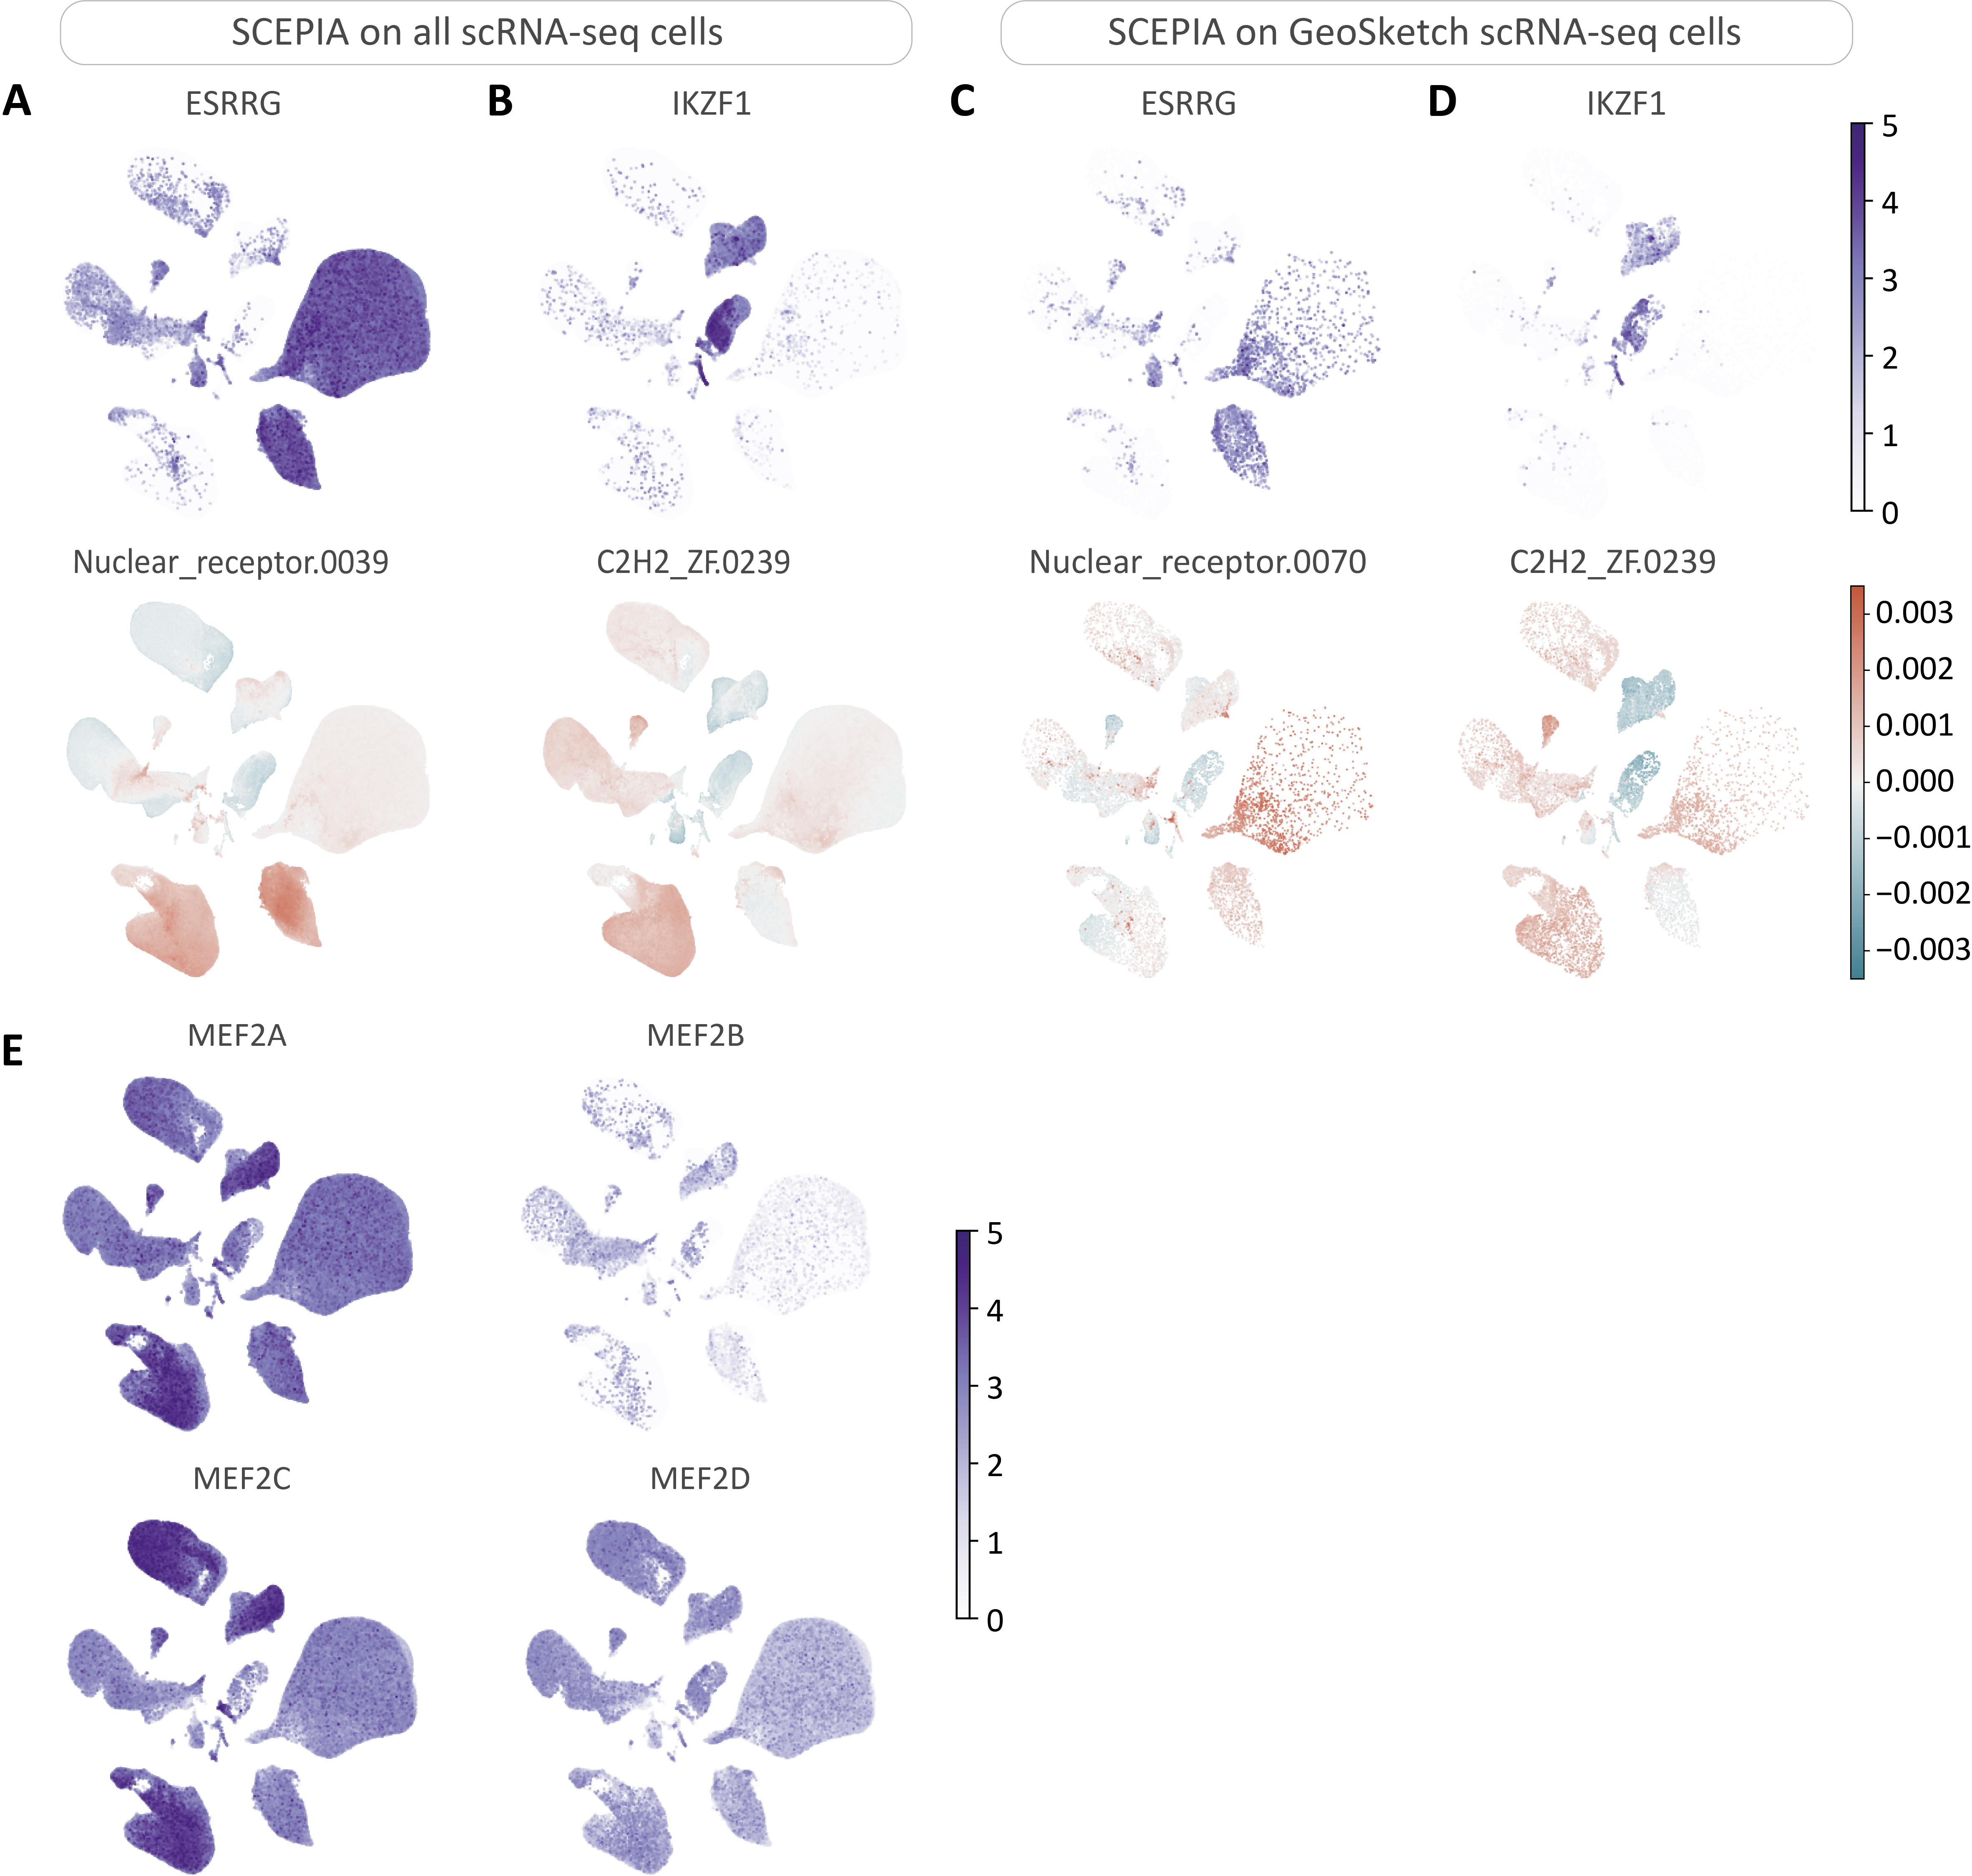
\includegraphics[width=\linewidth]{ch.scepia/imgs/SCEPIA_SCEPIAGEO_BiologicalExamples_SuppFig2_v2.png}
    \caption{Examples of SCEPIA and geosketch + SCEPiA run}
    \label{fig:scepia_features2}
\end{figure}
% \chapter{General Discussion}\thumbforchapter
\newpage

\section{The scientific dogma of the phylotypic stage}

\begin{shadequote}[c]{George Box}
All models are wrong, but some are useful.
\end{shadequote}

While historically the phylotypic stage has predominantly been examined and described through qualitative methods, the 21\textsuperscript{st} century started a paradigm shift towards a more quantitative and data-driven approach to understanding this phenomenon\cite{Chan2021}. The first notable quantitative investigation into the phylotypic stage was done by Bininda-Emonds \textit{et al.}, where they calculated temporal conservation as the order in which morphological embryonic features appear in vertebrates\cite{OlafRP2003}. However, it wasn't until the early 2010s that the field truly embraced quantitative methodologies with the simultaneous publication of two groundbreaking studies in Nature\cite{Kalinka2010, DomazetLoso2010}. In these works, Domazet-Lošo \textit{et al.} investigated the average developmental age of transcripts in \textit{D. rerio} and \textit{D. melanogaster}, whilst at the same time, Kalinka \textit{et al.} explored the temporal transcriptome similarities across different \textit{Drosophila} species. These molecular studies opened a new line of research to the quantitative basis of the phylotypic stage. The quantitative support for the phylotypic stage appears stronger and stronger with each new study. So strong, that we quickly forget all the nonconforming results.

The Transcriptome Age Index (TAI), as introduced by Domazet-Lošo \textit{et al.}, is a metric of the average evolutionary age of transcripts over time\cite{DomazetLoso2010}. In this study, evolutionary age is determined as the count of taxonomic branches that can be traced back to a gene. The central idea of the TAI is that temporal changes in the average transcript age provide insights into the degree of conservation during development. Domazet-Lošo \textit{et al.} found that both zebrafish and \textit{Drosophila} expressed the oldest transcriptome at their respective phylotypic stages and concluded that an old transcriptome marks the phylotypic phase. However, an independent re-analysis conducted by Piasecka \textit{et al.} raised some critical points about the methodology\cite{Piasecka2013}. Their investigation revealed that the TAI is heavily influenced by a relatively small subset of genes due to major differences in transcript levels per gene (transcriptomic data is notoriously heteroscedastic\cite{Rocke2001}). Log transforming the data, which is a standard processing step for this type of data, completely invalidates the results of the original study. One might expect such a dependency on data transformation to cast doubts on the reliability of the method. Surprisingly, the opposite appears to be true. The original study introducing the TAI has been cited 88 times between 2010 and 2013, but has been cited 359 times since Piasecka \textit{et al.}'s publication (covering the years 2014-2023). As it turns out, you can now analyze the data with and without transformation, and keep the results that reinforce your preferred hypothesis. A notable example of this is Wu \textit{et al.}'s study on Spiralian development\cite{Wu2019}. In their analysis of untransformed data for \textit{Crassostrea gigas}, \textit{Haliotis discus hannai}, and \textit{Perinereis aibuhitensis}, they claim to have found an inverse hourglass pattern of evolutionary conservation and speculate why spiralia have a different temporal selection pressure than other species. However, their supplementary data reveals a different pattern for \textit{Crassostrea gigas} after square root transformation, shifting from an inverse hourglass to a funnel shape. Remarkably, this crucial finding receives minimal attention in the study, with the authors merely stating that at least the transformed data does not show an hourglass-like pattern. Moreover, the transformed TAI of the other two species is not even shown, and upon closer inspection, it appears that the inverse hourglass pattern of \textit{Perinereis aibuhitensis} of untransformed data can simply be attributed to random noise. Where one should be careful with elaborate interpretations of this study, it has instead sparked an exchange among three influential evolutionary-developmental biologists - Pavel Tomanczak, Denis Duboule, and Andreas Hejnol - on Twitter (now X), about the universality of the hourglass model\cite{hejnoltwitter}. It is worth mentioning that Andreas Hejnol has authored two critical reviews about the methodology and design of previous studies that asserted the universality of the phylotypic stage\cite{Dunn2018,hejnol2016}.

The work of Barbara Piasecka, where she showed that the pattern of the TAI is caused by a subset of all genes was led by Marc Robinson-Rechavi. The main work of this study was not about the TAI, but about using a multitude of different metrics to estimate temporal evolutionary conservation. Their conclusion is that different metrics produce different results. In his personal blog, Marc Robinson-Rechavi concludes \say{First, that biology is complicated, and insisting on answers such as « the hourglass exists (and explains diverse data) » or « it doesn’t » may not be the best strategy. Second, that the technical details are very important}\cite{robinsonrechaviblog}. Marc Robinson-Rechavi's later career, however, appears to have diverged from his earlier conclusions. He has made assertive claims concerning the ortholog conjecture\cite{KryuchkovaMostacci2016} and the hourglass model of conservation\cite{Liu2020,Liu2021,marletaz2018}. A re-analysis by Casey Dunn, Andreas Hejnol, and others identified methodological issues with their analysis of the ortholog conjecture\cite{Dunn2018}, and in \textbf{chapter X} I discuss in detail the methodological problems of two of his studies related to the hourglass model.

In 2003, Bininda-Emonds \textit{et al.} conducted a quantitative study of the phylotypic stage, which was revisited seventeen years later by Gerardo A. Cordero \textit{et al}\cite{OlafRP2003, Cordero2020}. Both studies were about the quantitative temporal analysis of morphological characteristics. To the best of my knowledge, these are the only quantitative analyses of morphological characteristics with respect to the phylotypic stage. The initial findings of Bininda-Emonds \textit{et al}. revealed an unexpected inverse hourglass pattern in morphological rankings, a discovery that challenged the existing assumption of mid-development being the most conserved. However, it took seventeen years for a follow-up study, that surprisingly showed precisely the opposite - an hourglass pattern. Unfortunately, Cordero \textit{et al.} only comment that the difference between these two studies \textit{could} be caused by a difference in morphological characteristics, methodology, and species used, without any further analysis of the differences. They were correct in their assessment however, as in \textbf{chapter X} I show through simulations that the inverse hourglass pattern of Bininda-Emonds \textit{et al.} is caused by the methodology's sensitivity to edge effects, and does not represent biological signal.

In 2016, Levin \textit{et al.} introduced the transcriptomic inverse hourglass model as a potential method for distinguishing between different phyla\cite{Levin2016}. However, this study has been criticized by Casey Dunn and Andreas Hejnol for its lack of a within-phylum control\cite{hejnol2016} and incorrect statistical methods\cite{Dunn2018}. Given the ambitious claim of a "universal" phylotypic stage characterized by a high similarity within phyla but a low similarity between phyla, it is somewhat perplexing that these criticisms have not yet been addressed by Levin \textit{et al}. What makes the situation even more confusing is that another group of evolutionary developmental biologists compared the embryonic development of deuterostomes and the chordate amphioxus - a between-phyla comparison. Astonishingly, they uncovered an hourglass-like pattern\cite{PerezPosada2022}, directly contradicting Levin \textit{et al.}'s inverse hourglass model, but do not comment on this. In \textbf{Chapter XXX}, I present evidence that the transcriptomic inverse hourglass is a statistical artifact resulting from normalization rather than an accurate representation of temporal conservation. 

Yoav Mayshar \textit{et al.} studied the phylotypic stage and the hourglass model from a single-cell point of view\cite{Mayshar2023}. Their research involved a comparative analysis of cell type proportions during the development of rabbit and mouse embryos. However, in \textbf{Chapter X}, I show that both the rabbit time series as well as the mouse time series exhibit discontinuous patterns. These discontinuities influence the temporal correlations between the two species. Without better-distributed temporal sampling, a direct comparison with this data in relation to temporal conservation is not possible. Moreover, when there is a mid-developmental transition between two time-series, pairwise comparisons between these two time-series are visually similar to an hourglass. Thus confusingly, when comparing two time-series, if an hourglass is visible, this represents the inverse hourglass model. It seems that Mayshar \textit{et al.} fell for this pitfall, as they perceive their mid-developmental transition as confirming the traditional hourglass model. Perhaps even more surprising, is that no one cared to correct their misinterpretation when they published their preprint on Biorxiv and that the reviewers of Cell, one of the most prestigious journals, failed to notice it.

\begin{figure}
    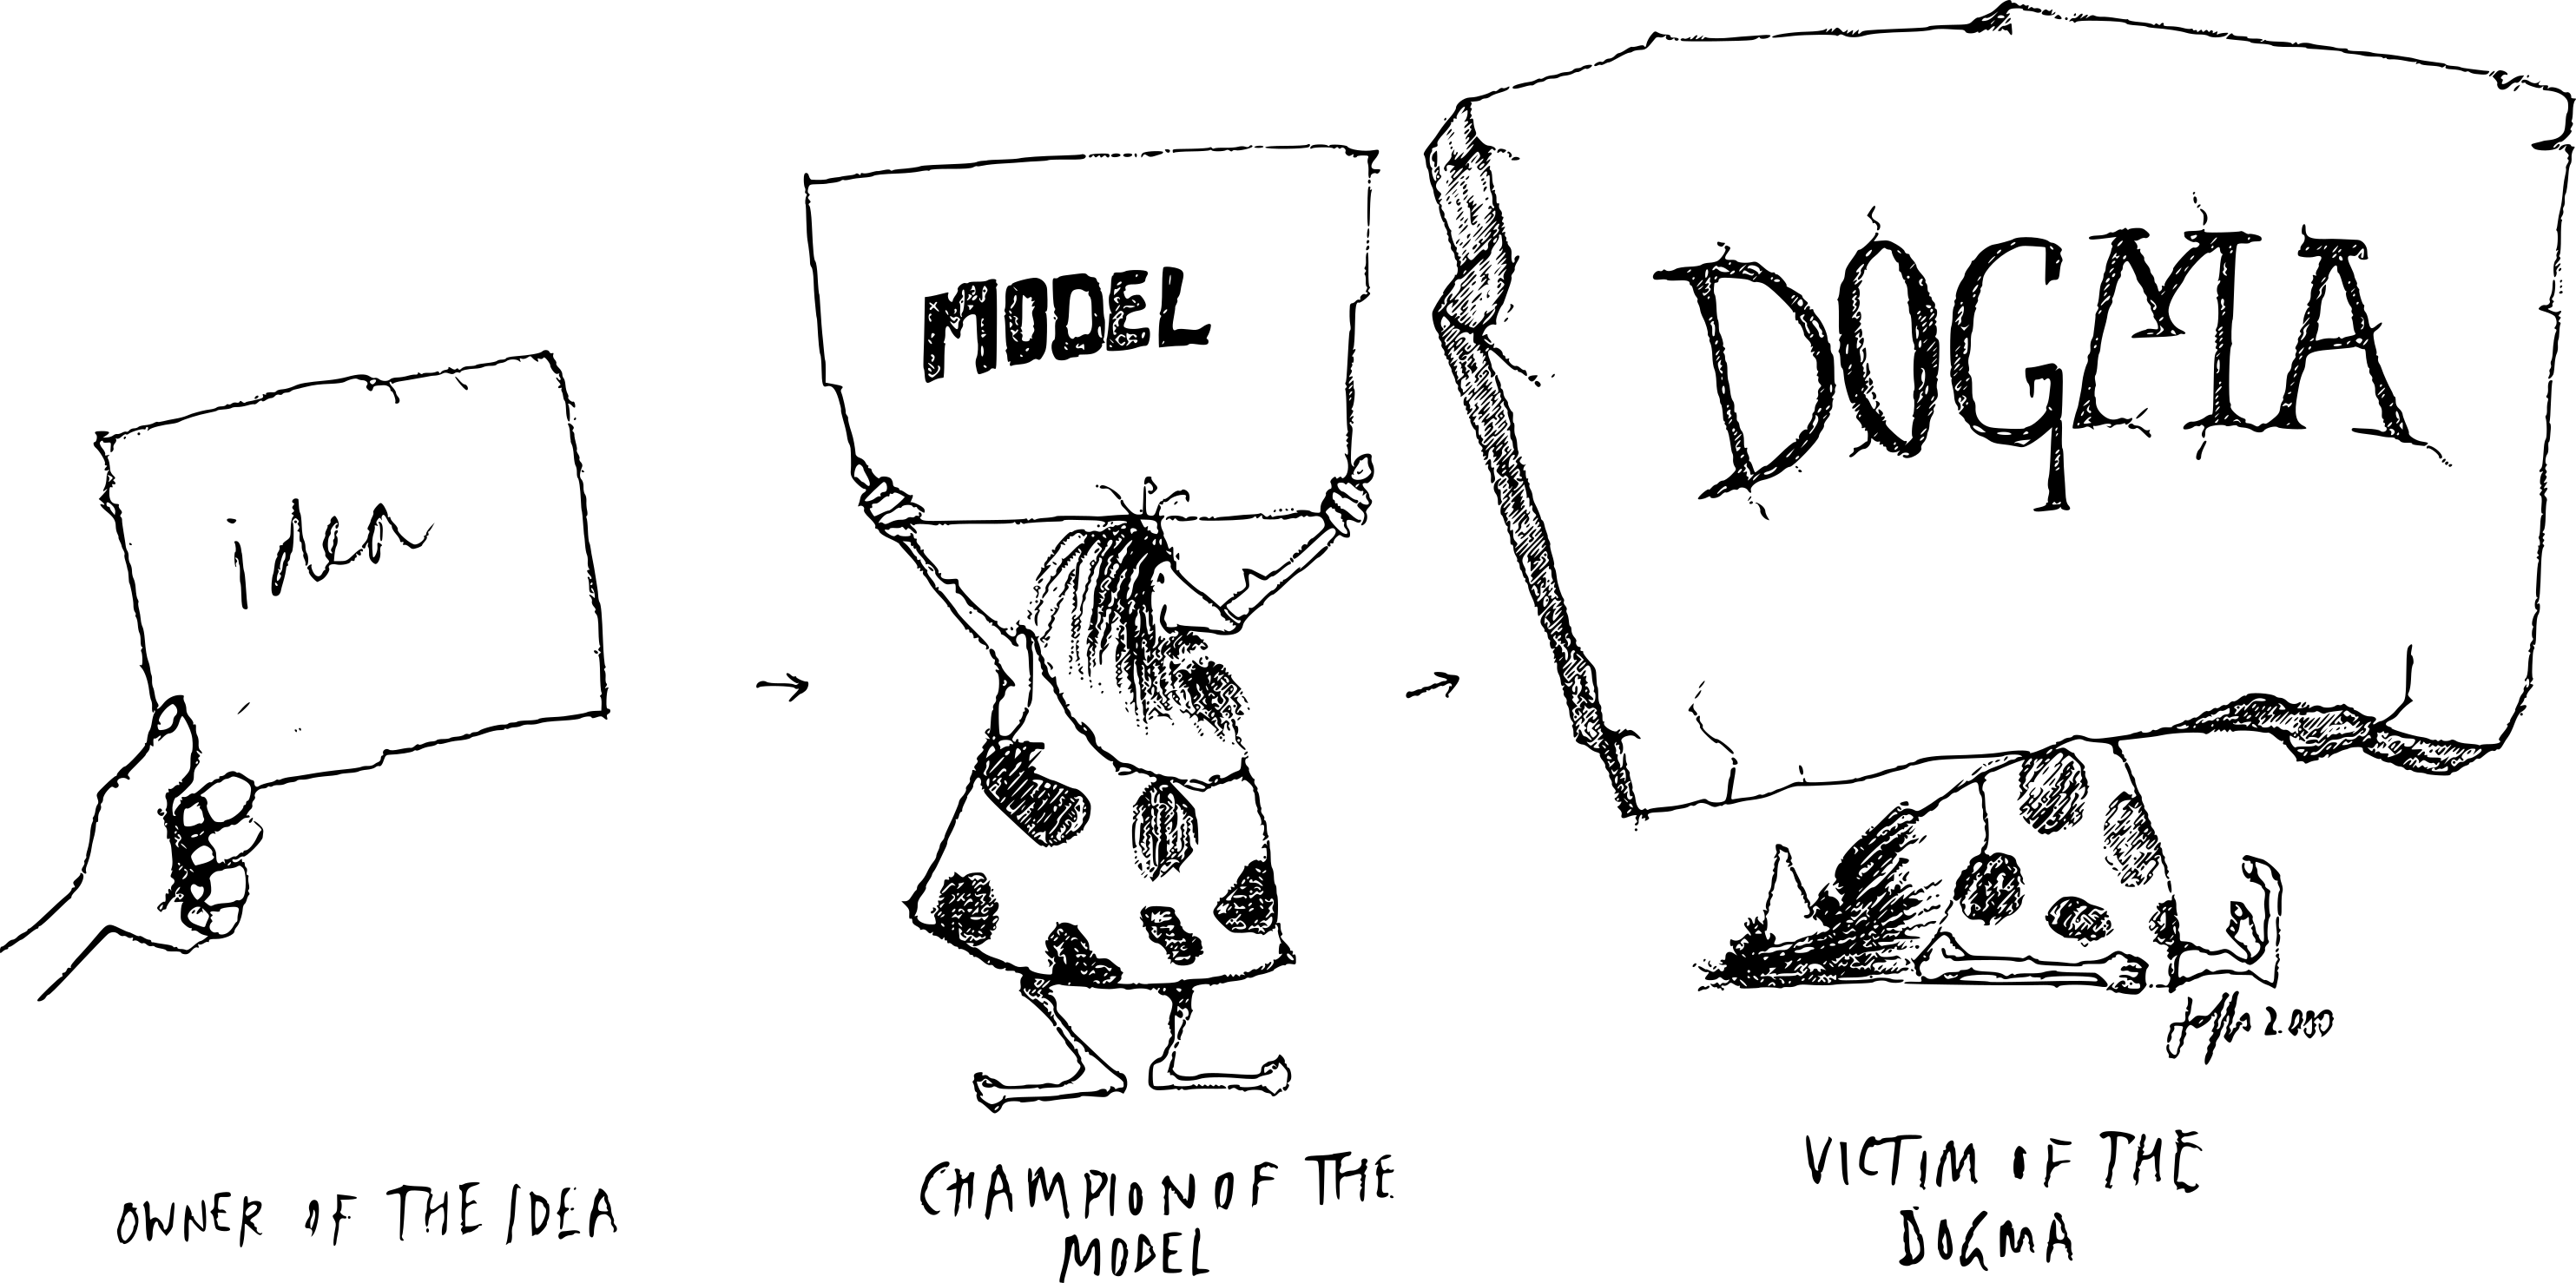
\includegraphics[width=\linewidth]{ch.discussion/imgs/dogma.png}
    \caption{\textbf{The phylotypic stage as a (crushing) scientific dogma?} \cite{Caveman2000}.}
    \label{fig:dogma}
\end{figure}

These examples highlight the dogmatic belief in the (non)existence of a phylotypic stage, and a reluctance to sincerely interact with each other's works. On top of that, in \textbf{chapter X and Y}, I discuss the methodological issues in comparative analyses concerning the phylotypic stage. The root problem is that the phylotypic stage and its related models are ill-defined, and as a consequence, there is a concerning lack of appropriate (statistical) controls in these studies. Is temporal conservation in these models present in comparisons within and between phyla? And is temporal conservation already observable when comparing a species against itself? By systematically addressing these ambiguities in previous studies through within-species, between-species, and between-phyla comparisons I show examples where the conclusions are not supported by the data. To summarize my main findings:
\begin{itemize}
    \item The transcriptomic hourglass-like pattern between zebrafish and frogs\cite{marletaz2018} can be explained by within-species correlations alone.
    \item     The transcriptomic between-phyla inverse hourglass pattern\cite{Levin2016} is a statistical artifact and can be reproduced by simulated data with no specific temporal conservation.
    \item The pattern of cell type proportion similarity between rabbits and mice\cite{Mayshar2023} can be explained by discontinuous temporal sampling.
    \item The \textit{Drosophila} enhancer conservation re-analysis results in a "mid-developmental" stage of maximum similarity, albeit at a different point than found by the original authors. Moreover, in \textbf{Chapter X} I highlight additional problems with the binarization of enhancers, and as such I do not endorse this methodology.
    \item  The morphological within-phylum inverse hourglass pattern is caused by edge effects and can be reproduced by simulated data with no specific temporal conservation.
\end{itemize}
\noindent
The null model for evolutionary embryonic development would be that there is no specific stage of higher or lower temporal conservation. Altogether, I have found little evidence to reject the null hypothesis of constant temporal conservation based on quantitative data, and thus see no reason to believe in a (molecular) phylotypic stage.

Moreover, in \textbf{Chapter X} I discuss further ambiguities in the models of the phylotypic stage. If a molecular phylotypic stage would exist, which features are expected to be conserved and which are not? The original observation that vertebrate embryos, perhaps, look more like each other \textit{externally} at certain points in development, says little about the whole-embryo molecular basis for this. While the morphological observations of Haeckel are almost 200 years old, there have been only two quantitative studies about the morphological phylotypic stage, and these two studies are in direct contradiction with each other. Instead, there appears to be a pursuit to find new (quantitative) methodologies that produce a more straight-forward confirmation of the existence of the phylotypic stage, such as embryonic lethality\cite{Uchida2018}, morphology\cite{OlafRP2003,Cordero2020}, DNA sequence conservation\cite{Piasecka2013,Quint2012,Liu2021} and activation order\cite{Uesaka2019}, cell type proportion\cite{Mayshar2023}, and whole-transcriptome similarity\cite{Piasecka2013,Irie2011,marletaz2018,Liu2020,Leong2021,PerezPosada2022,Kalinka2010}, with little sincere effort to integrate these results across studies. Of these methodologies, the whole-embryo transcriptome has become the most popular method to asses quantitative similarity. The implicit justification for this is that the transcriptome is an unbiased way to study genes during development. Still, the more cynical interpretation is that whole-embryo transcriptomic studies are the most confirming of our prior beliefs about the phylotypic stage. Even assuming the phylotypic stage exists, why would we expect to be able to measure such a complex phenomenon with such crude methods as observational studies and whole embryo sequencing? 

Throughout the course of scientific history, certain theories, such as taxonomic phyla and the phylotypic stage, have evolved from initial concepts into widely accepted truths, creating a demand for a molecular explanation along the way. However, a fundamental issue arises from the loose and ambiguous definitions on which these theories are based, leading to their lack of predictive power and falsifiability, rendering them, by Popperian standards, non-scientific in nature. For instance, the concept of phyla hinges on the notion that animals sharing a common basic body plan are part of the same phylum, yet paradoxically, the basic body plan is defined as the morphological characteristics shared by all animals within the same phyla\cite{BUDD2000}. The definition of the phylotypic stage is similarly ambiguous. Historically, the pharyngula stage\cite{BALLARD1981}, early somite embryo\cite{Alberch1993}, and the tail bud stage \cite{Slack1993} have all been proposed as the vertebrate phylotypic stage. In quantitative studies, the choice of definition in turn depends on which stage exhibits the highest quantitative conservation. Consequently, the pharyngula \cite{Irie2011,marletaz2018}, the early somite embryo \cite{DomazetLoso2010}, or simply the stage(s) with the highest conservation metric\cite{Kalinka2010,Cordero2020} have all been identified as phylotypic stages. Our current approach to studying the phylotypic stage, where we selectively include definitions and ignore nonconforming studies, is not only wrong but also not useful.

\section{gene regulatory network inference}

Gene regulatory network inference is bla bla. Many people do it. However current approaches perform poorly, barely any better than random. Here are some examples of poor performance (perhaps clinical trial performance?). As discussed in \textbf{Chapter XYZ}, the inclusion of multi-omics data, single-cell sequencing, and artificial neural networks when inferring gene regulatory networks should greatly increase their performance. 

Our golden standard is actual clinical trials! Our methods don't seem to work so well..?
% https://www.ncbi.nlm.nih.gov/pmc/articles/PMC6409418/
% https://journals.plos.org/plosmedicine/article?id=10.1371/journal.pmed.0020124
% https://www.cell.com/trends/genetics/fulltext/S0168-9525(21)00266-3

The inclusion of single-cell data is important because...,. Theoretically gives the cleanest data. But big issues with batch effects and sparsity. Also, they don't seem to work any better. Even though it is extremely important, fundamentally it is the least important or interesting of the three additions, but surprisingly seems to get the most attention.

More important is the inclusion of multiple modalities. The fundamental issue here is that it is wrong to assume that transcripts are all that we need. It ignores many important levels of regulation, such as post translational etc. On top of that, the poor relation between transcripts and proteins, means that our networks are formed on the wrong assumption that transcripts equal protein and/or on extremely noisy data. The correlation between protein expression and mRNA expression seems high (0.87) measured across cell types. However, genes with high protein expression generally have high mRNA expression. So it is easy to get high prediction. If you want to predict a single gene you get correlation of 0.41. Simpson's paradox?
https://www.nature.com/articles/nature23293
RNA-seq is used as a proxy for gene regulation, and simultaneously as a proxy for protein count/occurance. But transcripts are the measured effect of gene regulation. And transcipts correlate poorly. It was fine to try to make GRNs only on RNA-seq. We now know that does not work. (Stop doing it :) )
% https://www.biorxiv.org/content/10.1101/2023.05.23.541948v1
% https://twitter.com/nimwegenlab/status/1671923176626847744?s=12&t=oyB_faiBr8aHqHcjXZE50A

\begin{figure}[H]
    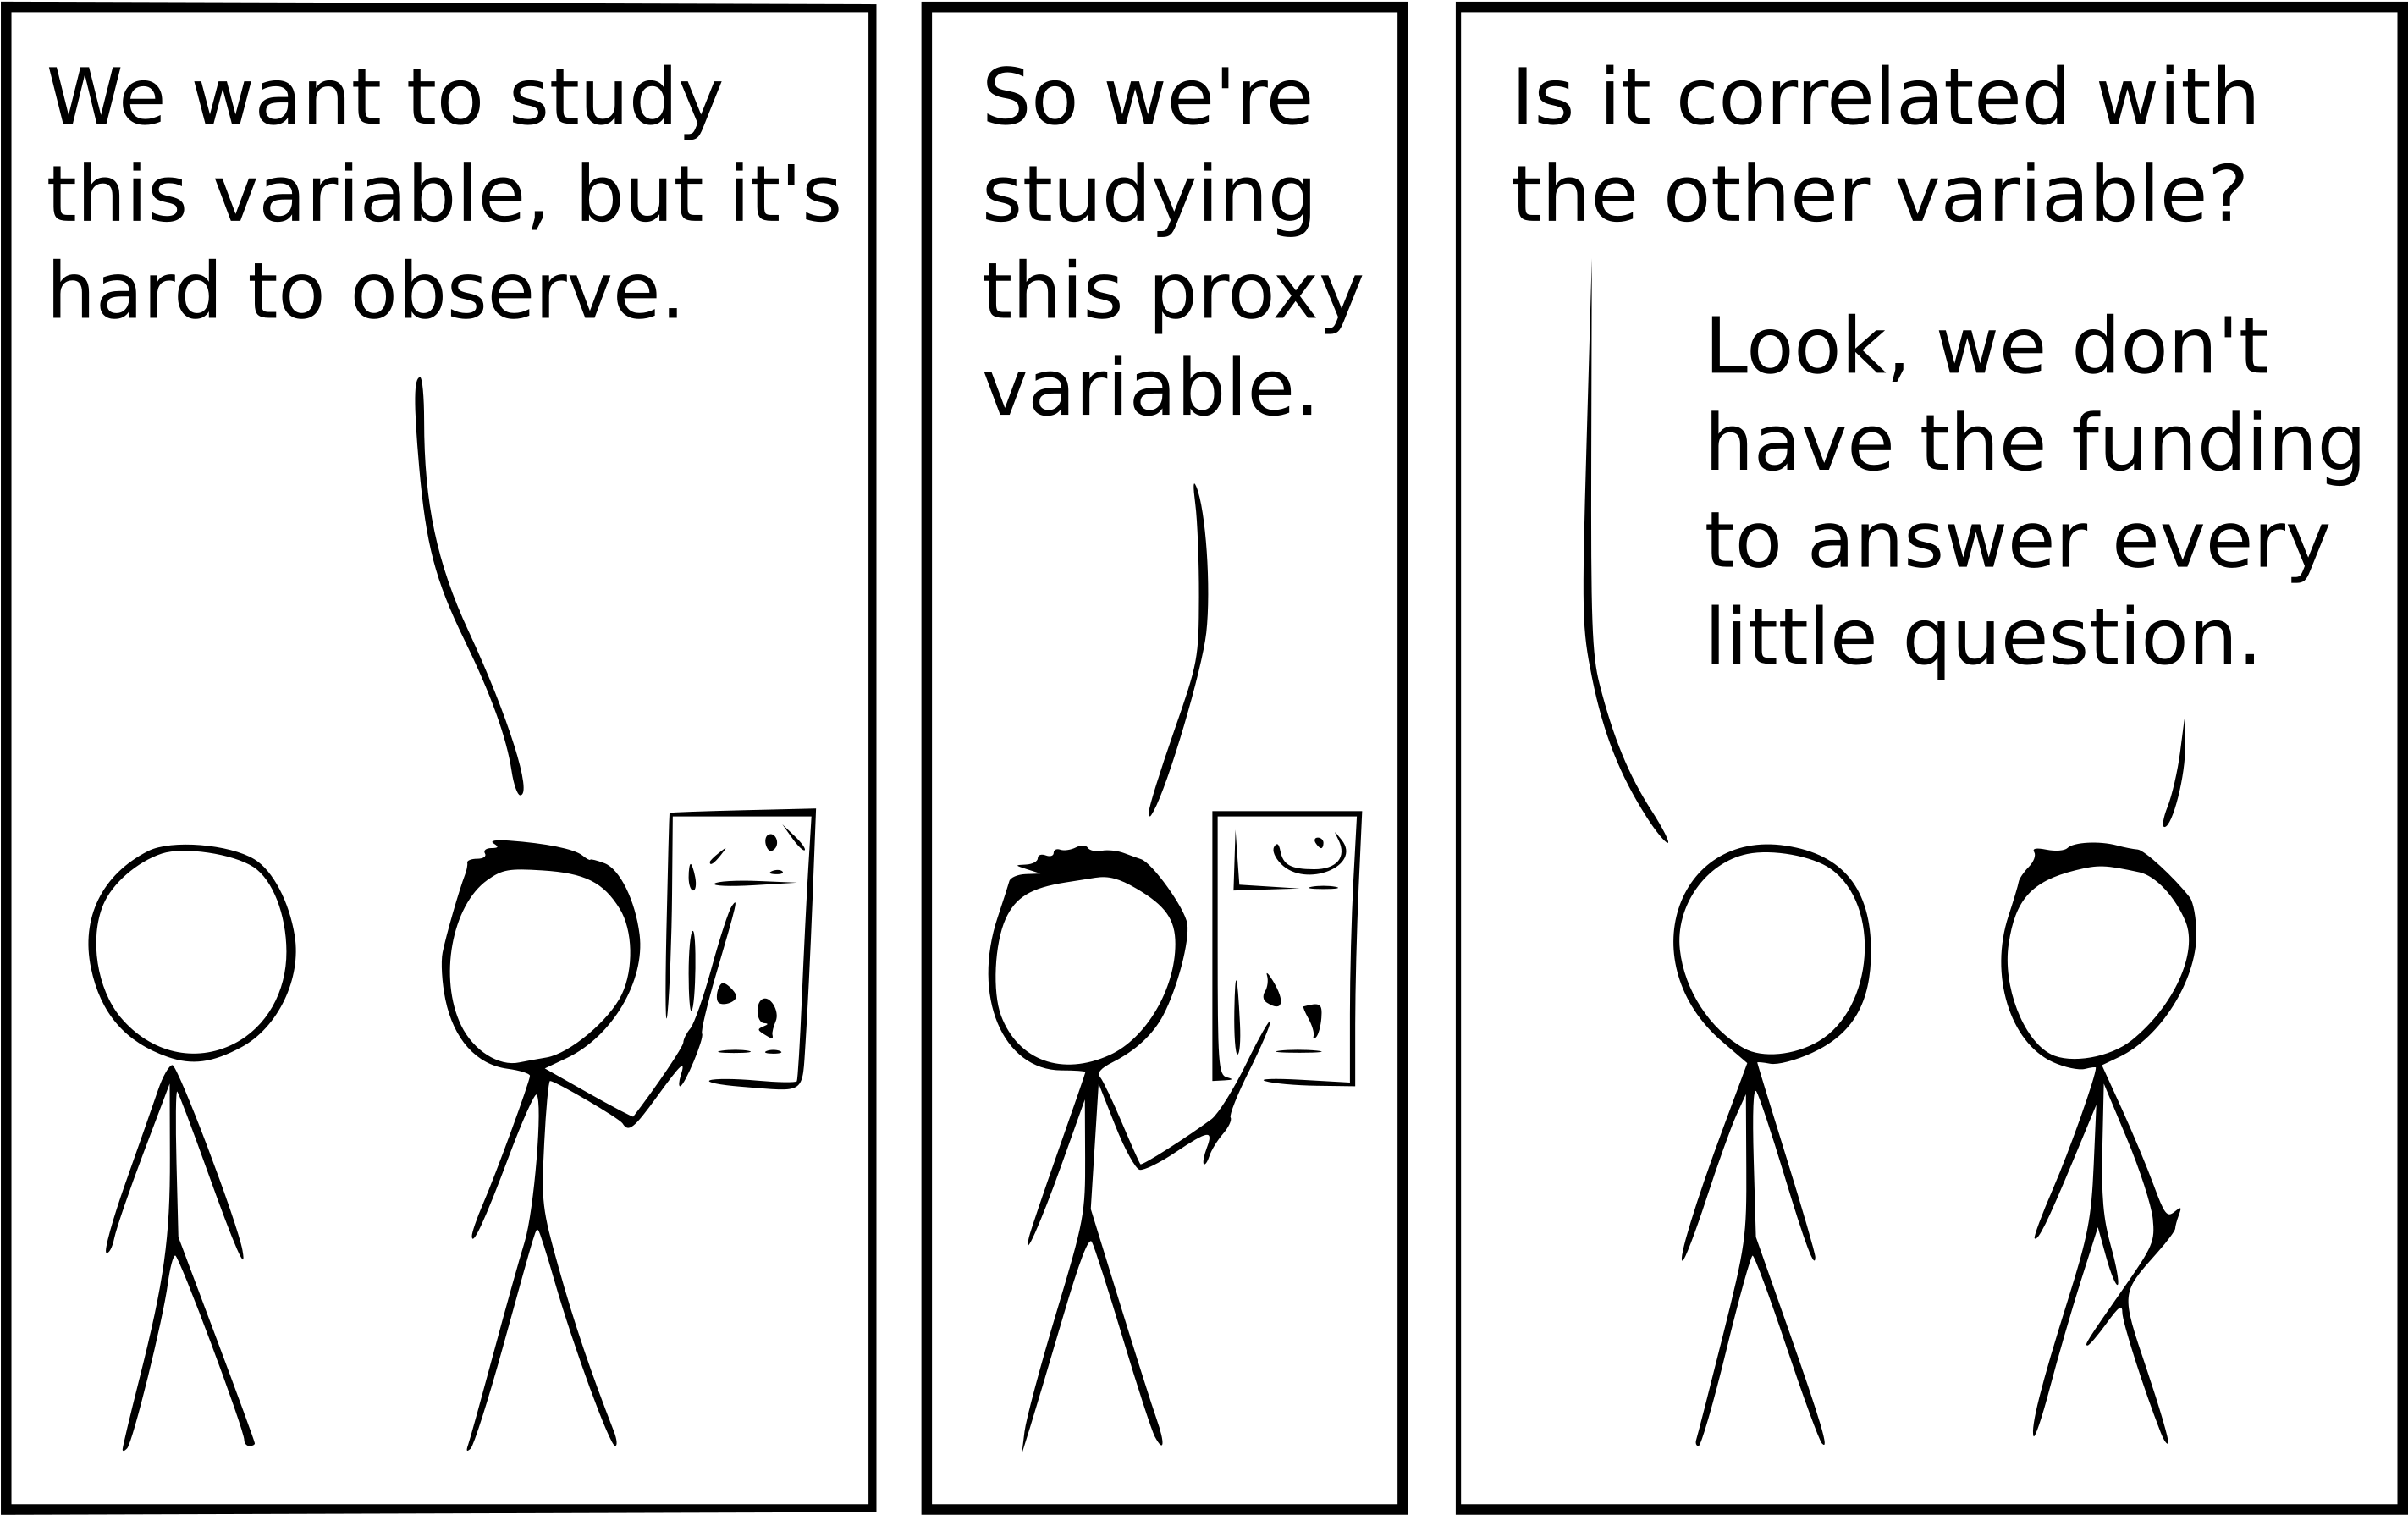
\includegraphics[width=\linewidth]{ch.discussion/imgs/xkcd_proxy.png}
    \caption{\textbf{RNA-seq is used as a proxy for gene regulation and protein expression}, but its relation to those is bad correlation TODO remains poorly understood. \textbf{xkcd}. URL: https://xkcd.com/2652}
    \label{fig:xkcd_proxy}
\end{figure}
The final addition is artificial neural networks. ANNs is perhaps the wrong term here, as it should not be about the tool. But about the idea. The idea is universal neural networks. As there is only a single set of instructions (DNA), we should model gene networks based on this idea. We should not try to infer the differential network between two cell states. Instead, we should strive to make a single network for all cell states. Fundamentally, this is more correct, and a network trained on the difference between two cell types is probably not capable of making predictions about perturbations. Moreover, making universal networks has the enormous advantage of having more data to train. (see schreiber avacodo).

Moreover, perhaps it is important to ask ourselves what is ultimately the goal of these GRNs? Do we care about having a map with all the arrows? Because the current correlation-based networks won't help us with differentiation networks. 

\section{Bioinformatics' technical debt}

Bioinformatics analyses are inherently complex due to the intricate nature of biology. This complexity is worsened by the dynamic and ever-evolving nature of these analyses, which continuously incorporate new technologies and insights. For instance, the number of new biomedical GitHub repositories is growing exponentially, with more than 3,000 new repositories opened in 2022 alone\cite{Patel2023}. Adding to this complexity is the use of outdated and idiosyncratic software and file formats. This in turn leads bioinformaticians to more easily make mistakes and do duplicate work. In software development, this problem is known as "technical debt". Technical debt is analogous to financial debt, where you borrow money and must eventually pay it back, including interest. I am of the opinion that in the field of bioinformatics, the technical debt has become so large that it has become prohibitive for analyses.

The most common file formats in bioinformatics have been designed in the 90s and 00s, and as such reflect the tools of their time. Perl and awk were popular languages for bioinformatics, and for this reason, file formats are mostly plain text and line-based. The sam, bam, bed, gff, and vcf file formats all specify genomic features and their location, and are a great example of ill-thought-through design. The bam- and bed-format are zero-indexed\cite{Li2009}, whilst the sam-, gff-, and vcf-format are one-indexed\cite{Li2009,Danecek2011}. This makes one-off errors between these formats extremely easy and incurs significant development time for anyone working with these formats. Moreover, as our understanding and analyses got more complex, it became necessary to express more complex relationships between features. This has led to a multitude of similar but incompatible gff versions and formats. The addition of these more complex relationships in gff files has made the format less suitable to be parsed line-by-line, which the format was originally designed for. An illustrative example highlighting the issues with positional formats is a tweet by Lior Pachter, where he asked if there is a citation for the gtf format. The most popular response covered the collective frustration of the field, stating \say{Ain’t no one gonna take responsibility for that mess}.
% https://twitter.com/lpachter/status/1719492098771300536

Another example of an outdated file format in bioinformatics is the fasta file format which was developed in 1985\cite{Lipman1985}. The fasta file format is a text-based format that represents nucleotide sequences or amino acid sequences, in which nucleotides and amino acids are represented using single-letter IUPAC codes. Its age initially shows because lines are typically split over 80 characters, as that was the maximum screen width of the past. The true problem with the fasta format is, however, that it can not naturally represent uncertainty at genomic locations. Single nucleotide polymorphisms are defined by their IUPAC codes, but uncertainties longer than a single nucleotide can not be naturally represented. The solution for this problem has been to append alternative sequences to the fasta. These sequences can then selectively be used in the downstream analysis. However, bwa mem(2)\cite{bwamem,bwamem2}, and Illumina Dragen are the only genomic aligners that currently support this, even though alternative regions have been added to the human genome since 2013. A switch to a graph-based genome format\cite{Li2020} is obvious and seems unavoidable, but has somehow been postponed by the bioinformatics community. More confusing than the outdated file format is the slow adoption of updated genome assemblies. For example, in 2023, Google Scholar identified 7,630 publications that utilized the older hg19 or grch37 genome assemblies (released in 2009), while there were only 8,960 publications that used the newer hg38 or grch38 assemblies (released in 2013). Notably, the T2T-CHM13 assembly (released in 2022) has only received 222 citations so far in 2023. A better genome assembly, not surprisingly, results in more accurate clinical discoveries \cite{Aganezov2022}. Ultimately, the slow adoption of updated genomes by the community and the limitations of the fasta format inhibit discoveries in the field of bioinformatics.

A project with significant technical debt is the Sequencing Read Archive (SRA), which shares enormous amounts of public sequencing data. The SRA has been essential for my doctoral studies, as I have relied solely on public data. For \textbf{chapter XXX}, we aimed to download all available human H3K27ac data (+/- 12,000 samples) from the SRA as a reference database. Processing these samples meant that we had to download 20TB from the SRA and spent approximately 300,000 CPU hours processing them on Cartesius, costing roughly €1,000 for the SRA\cite{amazon}, €9,000 for Cartesius, and emitting nearly one tonne of CO2\cite{CO2}. In the analysis that followed, however, it turned out that obtaining sample annotations, such as tissue or cell type, is challenging due to the lack of standardized metadata on the SRA. Even though third-party tools like MetaSRA\cite{Bernstein2017}, and PredictMEE\cite{Klie2021} have been developed to automatically infer this metadata, they did not manage to resolve my issues. In the end, we decided to discard the experiment, wasting an enormous amount of resources.

Not only is the SRA missing crucial metadata, but their sra-tools, a toolkit for downloading sequencing data, are also particularly difficult to use. As a consequence, many alternative tools have been developed for downloading data from the SRA, such as the SRA-explorer\cite{sraexplorer}, pysradb\cite{pysradb}, FetchFastQ\cite{galvez2022metadata}, nf-core/fetchngs\cite{fetchngs}, parallel-fastq-dump\cite{parallelfastq}, and finally our download-fastq workflow of seq2science\cite{seq2science} (see \textbf{chapter XXX}). The technical debt of the sra-tools, as in a poor sra-tools implementation, results in additional and unnecessary work, wasting the time and resources of others. Similarly, the submission of new sequencing data is notoriously complicated, causing people to make mistakes, which even leads to others developing tools to streamline this process\cite{Quiones2020}. During my doctoral studies, I have come across many instances of data being mislabeled or missing, consuming a considerable amount of my time, presumably because of the difficult upload process.

A similar case where the technical debt of one group extends to others is MACS2. MACS2 is one of the most popular tools in bioinformatics and is used to discover enriched regions in the genome, and has been cited more than 14,000 times\cite{Zhang2008}. MACS2 has been continuously developed since 2008, and its developers should get credit for this effort. Nevertheless, MACS2 is a particularly poorly designed and unoptimized software tool. The recommended way to use MACS2 in the case of ATAC-seq discards all mates from paired-end data, effectively removing half of the cleavage information\cite{Gaspar2018}. This can be overcome by removing the mate tag of reads after alignment, or by converting the bam alignment file to a bed and using that as input. Most users are however not aware of this unexpected implementation, resulting in a suboptimal set of called peaks. A similarly surprising design choice is that MACS2 did not support more than two replicates for over 10 years (until I added it in a pull request). As a practically identical, but better alternative to MACS2, Genrich has been developed by an independent group\cite{genrich}. 

Finally, the quickest developing part of molecular analyses currently is the field of single-cell analyses. As a consequence, the most technical debt is taken in these parts. Single-cell tools are usually implemented poorly, taking days to run and requiring enormous amounts of memory. The usual solution to this problem is not to improve the software implementation, but instead to increase the hardware capabilities. For instance, an ex-colleague of mine requested a massive 4TB of RAM for his computer at his new position. A particularly painful point of technical debt in the single-cell field is the implementation of the log fold change calculation of Seurat. Seurat calculates the log of the means (as opposed to the mean of the logs), which makes it sensitive to outliers and this implementation should be corrected. This results in vastly different outcomes depending on whether one used Seurat or any alternative tool such as Scanpy for their analysis. The bug was reported in November 2022, got an incomplete fix in March 2023, and as yet has not been fixed (https://github.com/satijalab/seurat/issues/6654). Seurat has been cited 7,699 times\cite{Butler2018}.

Taking \textit{deliberate} technical debt is okay. Oftentimes you have to develop fast, whilst it is not even clear whether something will work out. The problem with bioinformatics is, however, that a large part of the technical debt is taken inadvertently. I think the two main reasons for this are the lack of bioinformatics training (as mentioned in \textbf{chapter Z}), and the lack of interdepartmental collaborations on software. Two things that, in hindsight, were also missing during my doctoral studies. 

Because the field of bioinformatics is so young and rapidly becoming more important the supply of bioinformaticians is lacking behind their demand. This in turn leads to biologists starting bioinformatics analyses without formal training. This is somehow a widely accepted fact in the field, and even facilitated and encouraged by projects such as Galaxy\cite{galaxy}. In turn, bioinformaticians without formal training in programming, statistics, or modeling are developing tools and file formats, and doing analyses, which simply means that the quality and correctness of these tools and analyses are low. A clear example is the widespread use of Excel, which notoriously mangles gene names\cite{Zeeberg2004}. For example, the gene SEPT1 gets converted into September 1, and consequently, approximately $30\%$ of studies report mangled gene names by Excel in their supplementary files\cite{Abeysooriya2021}. Without exception, every time I thoroughly delved into the methodology of an analysis I found major issues, for example, \textbf{chapters \textbf{X} and Y} or \textbf{https://pubpeer.com/publications/1AA141AA501FF528C34DFF944CEF8E\#1}. It is surprising that the idea prevails that anyone should be able to do a bioinformatics analysis, whilst wet lab work is typically restricted to those who have undergone formal training. By not formally training the current and next generation of bioinformatics, we are hindering long-term progress in the field.
\begin{figure}[H]
    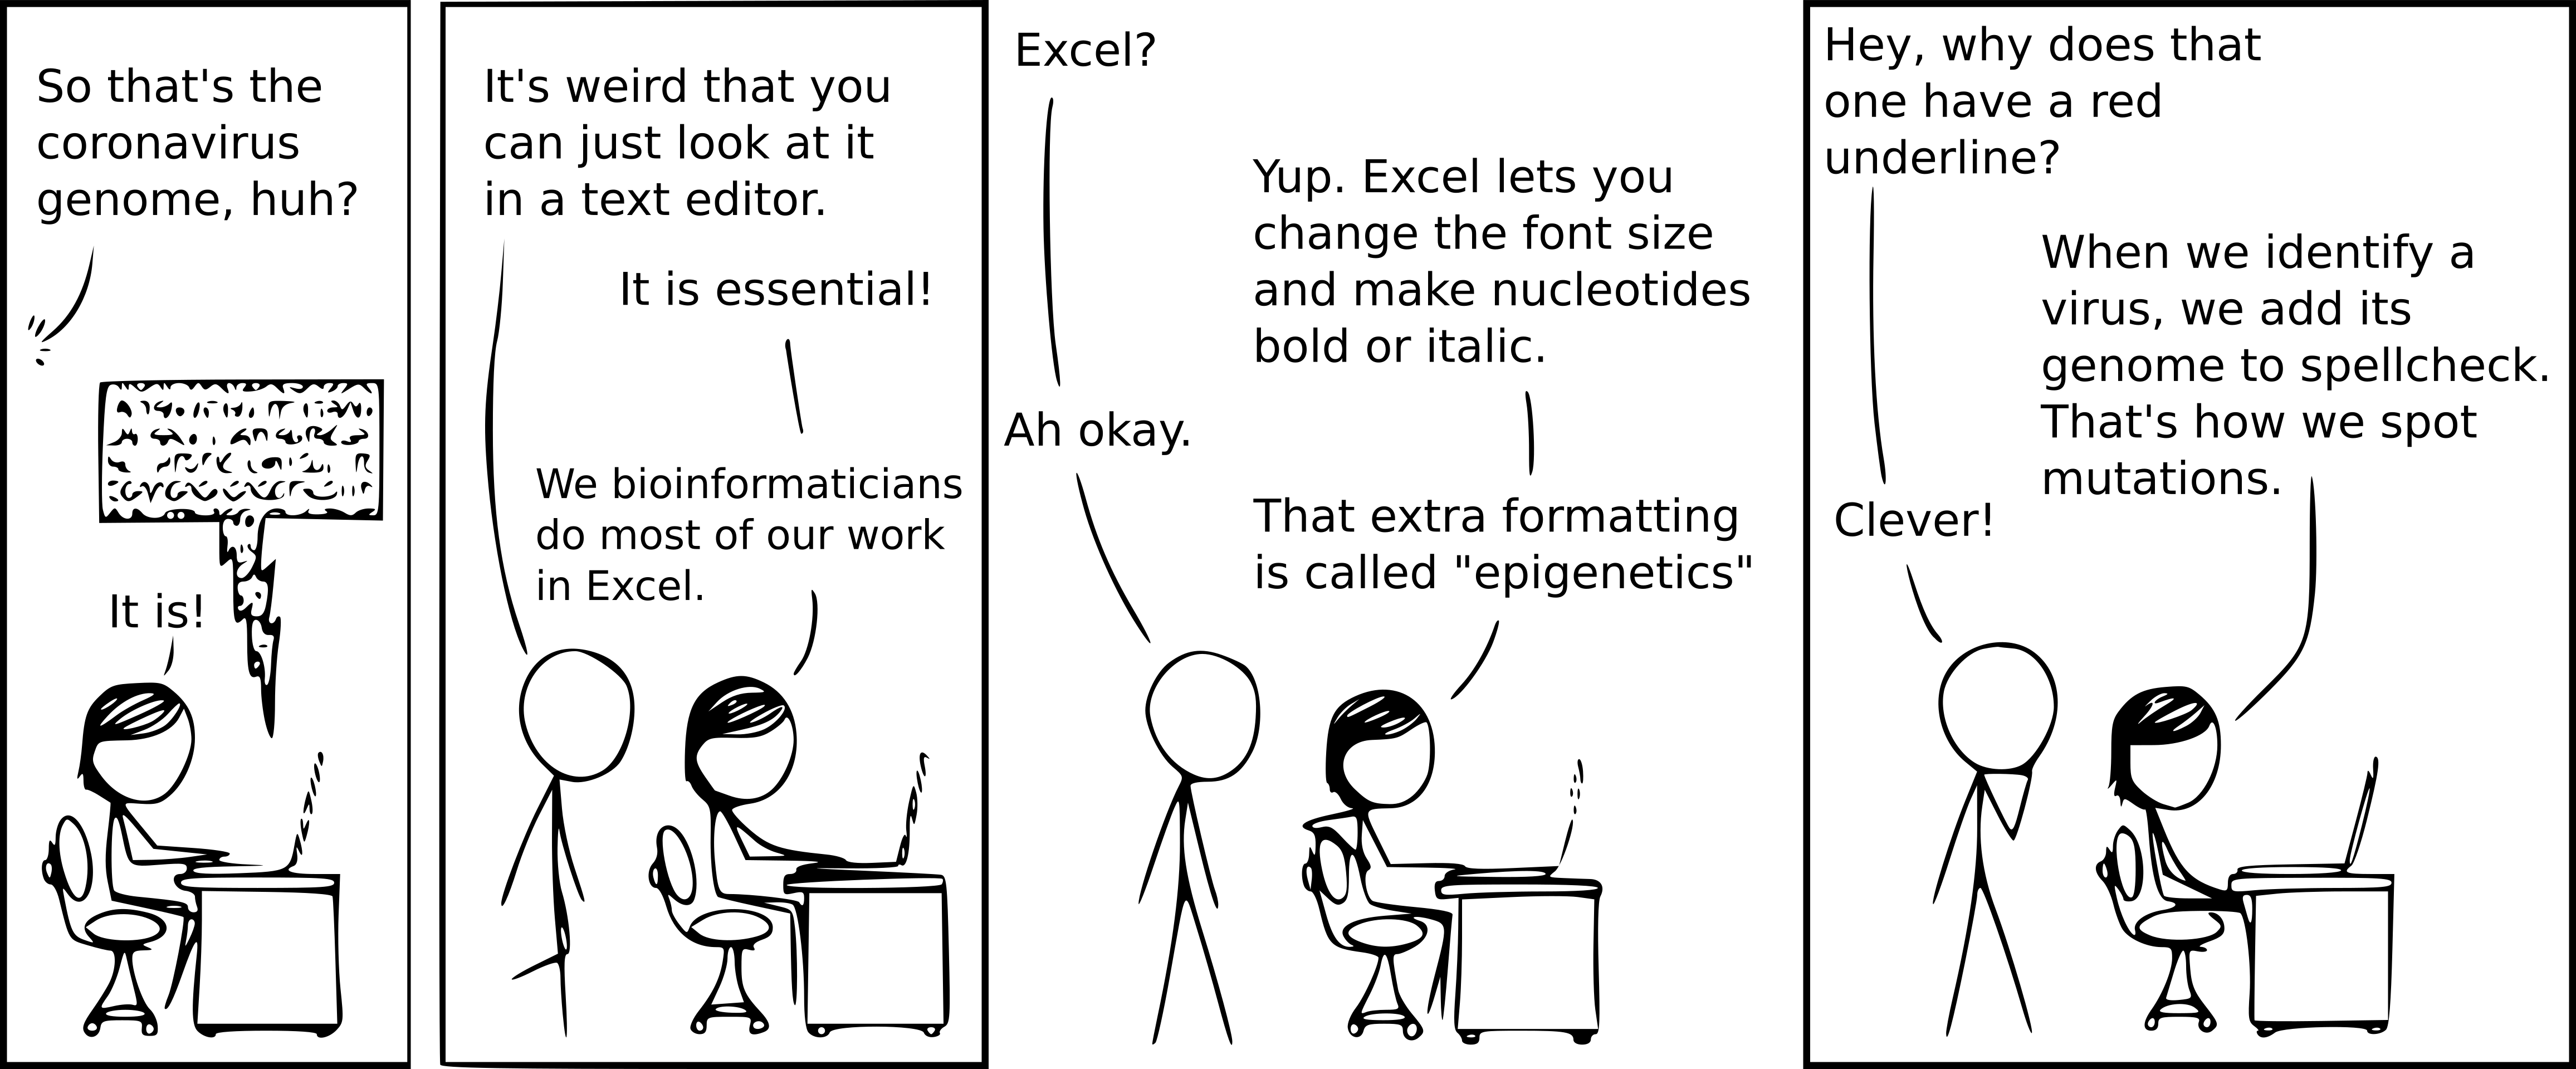
\includegraphics[width=\linewidth]{ch.discussion/imgs/xkcd_excel.png}
    \caption{\textbf{The use of Excel is surprisingly common in bioinformatics.} Adapted from xkcd. URL: https://xkcd.com/2298/}
    \label{fig:xkcd_excel}
\end{figure}
Another part of the problem is that most tools are developed independently, most of the time by a single doctoral student or postdoc. This has two major downsides. The first is that the maintenance of tools depends on individuals. If someone decides to leave academia, their tools, how useful they might be, will soon become obsolete as no one will maintain them. A clear example is the dissolution of the \say{van Heeringen} group, where soon tools such as genomepy\cite{genomepy}, gimmemotifs\cite{Bruse_2018}, ananse\cite{Xu_2020}, scepia, seq2science\cite{seq2science}, and qnorm\cite{qnorm} will become obsolete as they will no longer be maintained. Second, most tools are unnecessarily specialized for the task the developer is trying to solve. This in turn leads to many near-identical implementations that solve the same problem, for example, the many similar SRA-fastq downloading implementations mentioned before, including the seq2science implementation. These problems could be overcome if bioinformaticians would develop more interdepartmental collaborations. A software collaboration between multiple groups and expertise levels would ensure projects are not abandoned when a person leaves and that tools are useful for wider audiences.

In summary, despite the remarkable scientific breakthroughs facilitated by bioinformatics, the field is confronted with an increasingly taxing technical debt. This accumulating technical debt poses challenges for analyses, demanding immediate attention. For a long-term solution to bioinformatics' technical debt, it is necessary to normalize formal training and interdisciplinary collaborations - failure to do so risks inhibiting future advancements in the field.

\chapter{Appendix}\thumbforchapter
\newpage
\section{Summary in Dutch}

Een volwassen mens bestaat gemiddeld uit ongeveer 37 biljoen (37.000.000.000.000) cellen, die allemaal oorspronkelijk afkomstig zijn van \'e\'en enkele eicel. Tijdens de embryonale ontwikkeling vermenigvuldigt deze eicel zich veelvuldig, wat leidt tot steeds meer cellen en een toenemende diversiteit tussen deze cellen. Vroeg in de ontwikkeling ontstaan drie belangrijke kiemlijnen: het endoderm, ectoderm en mesoderm. Grof genomen ontwikkelen endodermale cellen zich tot de ingewanden, ectodermale cellen tot de huid en het zenuwstelsel, en mesodermale cellen tot het skelet, bloed en spieren. Hoewel al deze cellen hetzelfde DNA delen, verschillen ze uiteindelijk sterk van elkaar en voeren ze verschillende taken uit. Dit alles is mogelijk door een sterke regulatie van genexpressie. In dit proefschrift bespreek ik de computationele analyse van genexpressie, met een focus op transcriptieregulatie.

In \textbf{hoofdstuk 1} geef ik een inleiding over de onderwerpen die worden behandeld in dit proefschrift. Eerst behandel ik de regulatie van genexpressie via transcriptiefactoren, de relevantie van de staat van chromatine rondom genen, en geef ik een beknopte beschrijving van andere regulatoire mechanismen. Vervolgens bespreek ik hoe genexpressie wordt onderzocht, waarbij zowel het experimentele deel in het laboratorium als de daaropvolgende computationele analyse aan bod komen. Tot slot introduceer ik het vakgebied van evolutionaire ontwikkelingsbiologie (evo-devo). Evolutionair ontwikkelingsbiologen zijn geïnteresseerd in zowel de conservering als de verschillen in genregulatie tijdens de (embryonale) ontwikkeling tussen organismen.

In \textbf{hoofdstuk 2} bespreek ik de huidige stand van zaken rondom de analyse van genregulatoire netwerken (GRNs) en doe ik drie aanbevelingen aan het veld. Mijn eerste aanbeveling betreft het integreren van meerdere bronnen van informatie over genregulatie. Huidige GRNs zijn vaak uitsluitend gebaseerd op transcripten, terwijl het aantal transcripten slechts beperkt correleert met het aantal eiwitten van hetzelfde gen. Mijn tweede aanbeveling benadrukt het gebruik van single-cell technologie. Single-cell sequencing biedt een zuiverder signaal dan "bulk" sequencing, wat een positief effect kan hebben op GRN-analyse. Als laatste aanbeveling stel ik voor om universele GRN-modellen te ontwikkelen. De huidige netwerken zijn vaak gebaseerd op verschillen tussen twee condities, terwijl uiteindelijk dezelfde set instructies (DNA) wordt gedeeld door alle mogelijke GRNs.

In \textbf{hoofdstuk 3} introduceer ik seq2science, een computationeel hulpmiddel voor de preprocessing van data uit functionele genetica. Het biedt ondersteuning voor zowel de preprocessing van transcriptionele data (RNA-seq) als genomische data (ChIP-/ATAC-seq). Het is geïntegreerd met de meeste publieke databases en genereert een uitgebreid overzichtsrapport aan het einde van het proces.

In \textbf{hoofdstuk 4 en 5} behandel ik de definitie en analyse van het fylogenetische stadium. Het fylogenetische stadium is een fase tijdens de embryonale ontwikkeling waarin embryo's uit hetzelfde fylogenetische stam sterk op elkaar zouden lijken, wat heeft geleid tot het idee dat dit stadium evolutionair gezien geconserveerd is. Recentelijk zijn er kwantitatieve studies uitgevoerd naar zowel de morfologische als moleculaire gelijkenis tussen embryo's. In dit hoofdstuk bespreek ik de methodologische uitdagingen van deze analyses en heranalyseer ik eerdere studies. Zo laat ik onder andere zien dat de temporele conservering binnen soorten vaak vele malen sterker is dan tussen soorten, wat de analyse compliceert. Bovendien weerleg ik het omgekeerde zandlopermodel voor vergelijkingen tussen fylogenetische stammen als een statistisch artefact. Al met al is er weinig kwantitatief bewijs voor het bestaan van het fylogenetische stadium.

In \textbf{hoofdstuk 6} introduceer ik SCEPIA, een computationele methode die ondersteunt bij het schatten van de motiefactiviteit van transcriptiefactoren voor single-cell data. Aangezien transcripten slechts beperkt correleren met het aantal eiwitten van hetzelfde gen, koppelt SCEPIA eerst automatisch de transcriptie-informatie van een cel aan een referentiedatabase van H3K27ac. Door vervolgens op deze database de motiefactiviteit te schatten en deze te correleren met het aantal transcripten van dezelfde transcriptiefactor, levert SCEPIA aanzienlijk nauwkeurigere schattingen dan als je alleen naar transcripten kijken. Daarnaast valideer ik de resultaten van SCEPIA met behulp van een dataset van het menselijk hart.

Ten slotte vat ik in \textbf{hoofdstuk 7} mijn eerdere resultaten samen en bespreek ik ze in een bredere context. Ik benadruk daarbij de noodzaak van een systematische weergave van genregulatoire netwerken. Daarnaast uit ik kritiek op het onderzoek naar het fylogenetische stadium, waarbij ik voorbeelden geef van inconsistent gedrag van zowel onderzoekers als hun resultaten, en het naar mijn inzicht dogmatische geloof in het bestaan van het fylogenetische stadium. Tot slot deel ik mijn zorgen over de huidige stand van de bioinformatica, waarin veel computationele methoden en bestanden gebaseerd zijn op verourderde en simplistische aannames.

\section{Data management}
\cleartoleftpage
\section{Acknowledgements}

\vspace*{\fill}
\begin{figure}[H]
    \center
    
\includegraphics[width=0.8\linewidth]{ch.appendix/imgs/bigthanks.png}
\end{figure}
\vspace*{\fill}

\newpage

Thanks ppl

\newpage
\section{List of scientific publications}

\noindent
\underline{van der Sande M}*, Frölich S*, Schäfers T, Smits JGA, Snabel RR, Rinzema S, van Heeringen SJ. \textbf{Seq2science: an end-to-end workflow for functional genomics analysis.} PeerJ 11:e16380 \cite{seq2science}
\newline

\noindent
Frölich S, \underline{van der Sande M}, Schäfers T, van Heeringen SJ. \textbf{Genomepy: genes and genomes at your fingertips.} Bioinformatics 39 (3), btad119, 2023. \cite{Frlich2023}
\newline

\noindent
\underline{van der Sande M}*, Frölich* S, van Heeringen SJ. \textbf{Computational approaches to understand transcription regulation in development.} Biochemical Society Transactions 51 (1), 1-12, 2023. \cite{vanderSande2023}
\newline

\noindent
Wester RA, van Voorthuijsen L, Neikes HK, Dijkstra JJ, Lamers LA, Frölich S, \underline{van der Sande M}, Logie C, Lindeboom RGH, Vermeulen M. \textbf{Retinoic acid signaling drives differentiation toward the absorptive lineage in colorectal cancer.} Iscience 24 (12), 103444, 2021. \cite{Wester2021}
\newline

\noindent
Xu Q, Georgiou G, Frölich S, \underline{van der Sande M}, Veenstra GJC, Zhou H, van Heeringen SJ. \textbf{ANANSE: An enhancer network-based computational approach for predicting key transcription factors in cell fate determination.} Nucleic Acids Research 49 (14), 7966-7985, 2021. \cite{Xu_2020}
\newline

\noindent
Bright AR, van Genesen S, Li Q, Grasso A, Frölich S, \underline{van der Sande M}, van Heeringen SJ, Veenstra GJC.
\textbf{Combinatorial transcription factor activities on open chromatin induce embryonic heterogeneity in vertebrates.} The EMBO Journal 40 (9), e104913, 2021. \cite{Bright_2021}
\newline

\noindent
Vierboom MPM, Dijkman K, Sombroek CC, Hofman SO, Boot C, Vervenne RAW, Haanstra KG, \underline{van der Sande M}, van Emst L, Domínguez-Andrés J, Moorlag SJCFM, Kocken CHM, Thole J, Rodriguez E, Puentes E, Martes JHA, van Crevel R, Netea MG, Aguila N, Martin C, Verreck FAW. \textbf{Stronger induction of trained immunity by mucosal BCG or MTBVAC vaccination compared to standard intradermal vaccination.} Cell Reports Medicine 2 (1), 100185, 2021. \cite{Vierboom2021}
\newline

\noindent
\underline{van der Sande M}, Kraus Y, Houliston E, Kaandorp J. \textbf{A cell-based boundary model of gastrulation by unipolar ingression in the hydrozoan cnidarian Clytia hemisphaerica.}  Developmental biology 460 (2), 176-186, 2020. \cite{vanderSande2020}
\newline

\noindent
* These authors contributed equally to this work.

\newpage
\section{List of open-source scientific software contributions}

\noindent
\textbf{GimmeMotifs}: 17 merged Pull Requests; most notably the addition of the motif2factors command which automatically converts a motif database to any species based on orthology. Moreover, these PRs include numerous bug fixes and documentation improvements.
\newline

\noindent
\textbf{Snakemake}: 9 merged Pull Requests; most notably the addition of automated keyword unpacking and the addition of LockExpection, but also include numerous bug fixes and documentation improvements.
\newline

\noindent
\textbf{MultiQC}: 5 merged Pull Requests; with the addition of the BUStools module, the addition of show/hide buttons, and improvements to the MACS2 module. 
\newline

\noindent
\textbf{BioConda \& Conda-Forge}; maintaining 9 packages (seq2science, ngs-tools, kb-python, peaksql, pyseq-align, pretty\_html\_table, qnorm, iteround, and loompy).
\newline

\noindent
\textbf{Pysradb}: 4 merged pull requests; including performance improvement by multithreaded loading, and bug fixes.
\newline

\noindent
\textbf{Snakemake wrappers}. The addition and maintenance of the Genomepy and encode-download wrappers.
\newline

\noindent
\textbf{MACS2}: 1 merged pull request; which adds the option to include more than 2 replicates for peak calling.
\newline

\noindent
\textbf{gffread}: 1 merged pull request; which removes duplicate code.
\newline

\noindent
\textbf{fluff}: 1 merged pull request; fixing a bug concerning not correctly removing temporary files.
\newline

\noindent
\textbf{kbpython}: 1 merged pull request; extending the recognized nucleotides with the full IUPAC code.
\newline

% \begin{itemize}
%     \item GimmeMotifs: 17 merged pull requests with bug fixes, added functionality, and documentation changes.
%     \item Snakemake: 9 merged pull requests with bug fixes, added functionality, and documentation changes.
%     \item MultiQC: 5 merged pull requests with added functionality, added new and updated existing modules.
%     \item BioConda \& Conda-forge:  maintainer of 4 conda-forge and 5 bioconda packages.
%     \item Pysradb: 4 merged pull requests with performance improvements and bug fixes.
%     \item pyfaidx: 2 merged pull requests with added functionality.
%     \item MACS2: 1 merged pull request with added functionality (now accepts 3 or more replicates).
%     \item gffread: 1 merged pull request of code cleanup (code duplication removed).
%     \item fluff: 1 merged pull request of bug fix (temporary files not always removed).
%     \item kbpython: 1 merged pull request of added feature (IUPAC code extension).
%     \item Snakemake wrappers: genomepy and encode downloader
% \end{itemize}

\newpage
\section{Curriculum Vitae}

Maarten van der Sande was born on August 13\textsuperscript{th} 1993, in the municipality of Renkum, the Netherlands. After completing his secondary education at Dorenweerd College, he started his bachelor's at the Universiteit van Amsterdam. Here, he simultaneously obtained two bachelor's degrees, one in Biology, and one in Liberal Arts and Sciences. Maarten, however, spent most of his time doing extracurricular activities such as competitive rowing, race biking, fencing, and finding his way home after a party. He finished his studies with a master's degree in Computational Science, a joint program of the Universiteit van Amsterdam and the Vrije Universiteit. At this time Maarten developed a healthy aversion to busy work, like writing Curriculum Vitae sections for PhD theses. After his studies in Amsterdam, Maarten went on to get a PhD degree at the Radboud Universiteit. Here, under the supervision of Simon van Heeringen, Maarten studied the computational analysis of transcription regulation during (evolutionary) development. During this time, Maarten also conducted aerodynamic field tests between Nijmegen and Wageningen, and concluded that he is particularly accident-prone. In December 2023, Maarten started a new job as a bioinformatician at Solynta, the world's most innovative potato breeding company.

% \fakesection{references}
\section{references}

\setlength\bibitemsep{1pt}
\renewcommand*{\bibfont}{\scriptsize}
\printbibliography[heading=none]



\end{document}
